% Options for packages loaded elsewhere
\PassOptionsToPackage{unicode}{hyperref}
\PassOptionsToPackage{hyphens}{url}
\documentclass[
]{book}
\usepackage{xcolor}
\usepackage{amsmath,amssymb}
\setcounter{secnumdepth}{-\maxdimen} % remove section numbering
\usepackage{iftex}
\ifPDFTeX
  \usepackage[T1]{fontenc}
  \usepackage[utf8]{inputenc}
  \usepackage{textcomp} % provide euro and other symbols
\else % if luatex or xetex
  \usepackage{unicode-math} % this also loads fontspec
  \defaultfontfeatures{Scale=MatchLowercase}
  \defaultfontfeatures[\rmfamily]{Ligatures=TeX,Scale=1}
\fi
\usepackage{lmodern}
\ifPDFTeX\else
  % xetex/luatex font selection
\fi
% Use upquote if available, for straight quotes in verbatim environments
\IfFileExists{upquote.sty}{\usepackage{upquote}}{}
\IfFileExists{microtype.sty}{% use microtype if available
  \usepackage[]{microtype}
  \UseMicrotypeSet[protrusion]{basicmath} % disable protrusion for tt fonts
}{}
\makeatletter
\@ifundefined{KOMAClassName}{% if non-KOMA class
  \IfFileExists{parskip.sty}{%
    \usepackage{parskip}
  }{% else
    \setlength{\parindent}{0pt}
    \setlength{\parskip}{6pt plus 2pt minus 1pt}}
}{% if KOMA class
  \KOMAoptions{parskip=half}}
\makeatother
\usepackage{graphicx}
\makeatletter
\newsavebox\pandoc@box
\newcommand*\pandocbounded[1]{% scales image to fit in text height/width
  \sbox\pandoc@box{#1}%
  \Gscale@div\@tempa{\textheight}{\dimexpr\ht\pandoc@box+\dp\pandoc@box\relax}%
  \Gscale@div\@tempb{\linewidth}{\wd\pandoc@box}%
  \ifdim\@tempb\p@<\@tempa\p@\let\@tempa\@tempb\fi% select the smaller of both
  \ifdim\@tempa\p@<\p@\scalebox{\@tempa}{\usebox\pandoc@box}%
  \else\usebox{\pandoc@box}%
  \fi%
}
% Set default figure placement to htbp
\def\fps@figure{htbp}
\makeatother
\setlength{\emergencystretch}{3em} % prevent overfull lines
\providecommand{\tightlist}{%
  \setlength{\itemsep}{0pt}\setlength{\parskip}{0pt}}
\usepackage{bookmark}
\IfFileExists{xurl.sty}{\usepackage{xurl}}{} % add URL line breaks if available
\urlstyle{same}
\hypersetup{
  hidelinks,
  pdfcreator={LaTeX via pandoc}}

\author{}
\date{}

\begin{document}
\frontmatter

\mainmatter
\chapter{APLIKASI KOMPUTER}\label{aplikasi-komputer}

\begin{figure}
\centering
\pandocbounded{\includegraphics[keepaspectratio]{images/UNY.png}}
\caption{images/UNY.png}
\end{figure}

Disusun Oleh

Nama : Isni Azizah Utami

Kelas : Matematika B 2023

NIM: 23030630016

\chapter{KATA PENGANTAR}\label{kata-pengantar}

Puji syukur kami panjatkan kepada Tuhan Yang Maha Esa, karena berkat rahmat dan karunia-Nya, buku ini dapat terselesaikan dengan baik. Buku ini disusun sebagai panduan praktis mengenai penggunaan \emph{Engineering Mathematics Toolbox} (EMT) dalam penerapan matematika di berbagai bidang teknik dan sains.

Dalam perkembangan ilmu pengetahuan dan teknologi yang semakin pesat, penggunaan perangkat lunak atau software dalam proses pemecahan masalah matematika menjadi sangat penting. EMT adalah salah satu software yang dirancang untuk mempermudah perhitungan matematika, baik dalam analisis numerik, aljabar, statistik, hingga pemodelan matematika yang lebih kompleks. Dengan antarmuka yang intuitif dan berbagai fitur yang lengkap, EMT memberikan solusi praktis bagi para akademisi, peneliti, maupun praktisi di dunia teknik dan sains.

Buku ini bertujuan untuk memberikan pemahaman yang lebih dalam mengenai bagaimana software EMT dapat digunakan untuk menyelesaikan berbagai permasalahan matematika. Kami berharap buku ini dapat menjadi referensi yang berguna bagi pembaca yang ingin memperdalam pengetahuan tentang teknik-teknik pemrograman matematika, analisis numerik, serta pemodelan matematika menggunakan software EMT. Buku ini disusun dengan pendekatan yang sistematis dan mudah dipahami, dilengkapi dengan contoh aplikasi yang relevan agar pembaca dapat langsung mengaplikasikan pengetahuan yang diperoleh.

Kami menyadari bahwa buku ini masih jauh dari sempurna, oleh karena itu kritik dan saran dari pembaca sangat kami harapkan untuk perbaikan di masa mendatang. Semoga buku ini dapat memberikan manfaat yang sebesar-besarnya bagi para pembaca dalam meningkatkan pemahaman dan keterampilan mereka dalam menggunakan software EMT di bidang matematika.

Akhir kata, kami mengucapkan terima kasih kepada semua pihak yang telah memberikan dukungan, baik berupa materi, waktu, maupun pemikiran dalam penyusunan buku ini.

Selamat membaca dan semoga buku ini bermanfaat!

Penulis

\chapter{EMT untuk Perhitungan Aljabar}\label{emt-untuk-perhitungan-aljabar}

Pada notebook ini Anda belajar menggunakan EMT untuk melakukan berbagai perhitungan terkait dengan materi atau topik dalam Aljabar. Kegiatan yang harus Anda lakukan adalah sebagai berikut:

\begin{enumerate}
\def\labelenumi{\arabic{enumi}.}
\tightlist
\item
  Membaca secara cermat dan teliti notebook ini Menerjemahkan teks bahasa Inggris ke bahasa Indonesia;
\item
  Mencoba contoh-contoh perhitungan (perintah EMT) dengan cara meng-ENTER setiap perintah EMT yang ada (pindahkan kursor ke baris perintah)
\item
  Jika perlu Anda dapat memodifikasi perintah yang ada dan memberikan keterangan / penjelasan tambahan terkait hasilnya.
\item
  Menyisipkan baris-baris perintah baru untuk mengerjakan soal-soal Aljabar dari file PDF yang saya berikan;
\item
  Memberi catatan hasilnya.
\item
  Jika perlu tuliskan soalnya pada teks notebook (menggunakan format LaTeX).
\item
  Gunakan tampilan hasil semua perhitungan yang eksak atau simbolik dengan format LaTeX. (Seperti contoh-contoh pada notebook ini.)
\end{enumerate}

\section{Contoh pertama}\label{contoh-pertama}

Menyederhanakan bentuk aljabar: \[6x^{-3}y^5\times -7x^2y^{-9}\]\textgreater\$\&6*x\textsuperscript{(-3)*y}5*-7*x\textsuperscript{2*y}(-9)

\[-\frac{42}{x\,y^4}\]Menjabarkan: \[(6x^{-3}+y^5)(-7x^2-y^{-9})\] \textgreater\$\&showev('expand((6*x\textsuperscript{(-3)+y}5)*(-7*x\textsuperscript{2-y}(-9))))

\[{\it expand}\left(\left(-\frac{1}{y^9}-7\,x^2\right)\,\left(y^5+  \frac{6}{x^3}\right)\right)=-7\,x^2\,y^5-\frac{1}{y^4}-\frac{6}{x^3  \,y^9}-\frac{42}{x}\]

\section{Baris Perintah}\label{baris-perintah}

Baris perintah Euler terdiri dari satu atau beberapa perintah Euler diikuti dengan titik koma ``;'' atau koma ``,''. Titik koma mencegah pencetakan hasil. Koma setelah perintah terakhir dapat dihilangkan. Baris perintah berikut hanya akan mencetak hasil ekspresi, bukan tugas atau perintah format.

\textgreater r:=2; h:=4; pi*r\^{}2*h/3

\begin{verbatim}
16.7551608191
\end{verbatim}

Perintah harus dipisahkan dengan yang kosong. Baris perintah berikut mencetak dua hasilnya.

\textgreater pi*2*r*h, \%+2*pi*r*h

Ingat tanda \% menyatakan hasil perhitungan terakhir sebelumnya

\begin{verbatim}
50.2654824574
100.530964915
\end{verbatim}

Baris perintah dieksekusi dalam urutan yang ditekan pengguna kembali. Jadi Anda mendapatkan nilai baru setiap kali Anda menjalankan baris kedua.

\textgreater x := 1; \textgreater x := cos(x)

nilai cosinus (x dalam radian)

\begin{verbatim}
0.540302305868
\end{verbatim}

\textgreater x := cos(x)

\begin{verbatim}
0.857553215846
\end{verbatim}

Jika dua garis terhubung dengan ``\ldots{}'' kedua garis akan selalu dieksekusi secara bersamaan.

\textgreater x := 1.5; \ldots{}\\
\textgreater{} x := (x+2/x)/2, x := (x+2/x)/2, x := (x+2/x)/2,

\begin{verbatim}
1.41666666667
1.41421568627
1.41421356237
\end{verbatim}

Ini juga merupakan cara yang baik untuk menyebarkan long command pada dua atau lebih baris. Anda dapat menekan Ctrl+Return untuk membagi garis menjadi dua pada posisi kursor saat ini, atau Ctrl+Back untuk menggabungkan garis.

Sedangkan untuk fold semua multi-garis tekan Ctrl + L. Kemudian garis-garis berikutnya hanya akan terlihat, jika salah satunya memiliki fokus. Untuk fold satu multi-baris, mulailah baris pertama dengan ``\%+''.

\textgreater\%+ x=4+5; \ldots{}\\
\textgreater{} // This line will not be visible once the cursor is off the line

A line starting with \%\% will be completely invisible.

\begin{verbatim}
81
\end{verbatim}

Euler Math Toolbox mendukung loop di baris perintah, selama mereka masuk ke dalam satu baris atau multi-baris. Dalam program, pembatasan ini tidak berlaku, tentu saja. Untuk informasi lebih lanjut lihat pengantar berikut.

\textgreater x=1; for i=1 to 5; x := (x+2/x)/2, end;

menghitung akar 2

\begin{verbatim}
1.5
1.41666666667
1.41421568627
1.41421356237
1.41421356237
\end{verbatim}

Tidak apa-apa untuk menggunakan multi-line. Pastikan baris diakhiri dengan ``\ldots{}''.

\textgreater x := 1.5; // tambahkan komentar disini seblum \ldots{}\\
\textgreater{} repeat xnew:=(x+2/x)/2; until xnew\textasciitilde=x; \ldots{}\\
\textgreater{} x := xnew; \ldots{}\\
\textgreater{} end; \ldots{}\\
\textgreater{} x,

\begin{verbatim}
1.41421356237
\end{verbatim}

Struktur bersyarat juga berfungsi.

\textgreater if E\textsuperscript{pi\textgreater pi}E; then ``Thought so!'', endif;

\begin{verbatim}
Thought so!
\end{verbatim}

Saat Anda menjalankan perintah, kursor dapat berada di posisi mana pun di baris perintah. Anda dapat kembali ke perintah sebelumnya atau melompat ke perintah berikutnya dengan tombol panah. Atau Anda dapat mengklik ke bagian komentar di atas perintah untuk menuju ke perintah.

Saat Anda menggerakkan kursor di sepanjang garis, pasangan tanda kurung atau kurung buka dan tutup akan disorot. Dan juga, perhatikan baris status. Setelah kurung buka fungsi sqrt(), baris status akan menampilkan teks bantuan untuk fungsi tersebut. Jalankan perintah dengan tombol kembali.

\textgreater sqrt(sin(10°)/cos(20°))

\begin{verbatim}
0.429875017772
\end{verbatim}

Untuk melihat bantuan untuk perintah terbaru, buka jendela bantuan dengan F1. Di sana, Anda dapat memasukkan teks untuk dicari. Pada baris kosong, bantuan untuk jendela bantuan akan ditampilkan. Anda dapat menekan escape untuk menghapus garis, atau untuk menutup jendela bantuan.

Anda dapat mengklik dua kali pada perintah apa pun untuk membuka bantuan untuk perintah ini. Coba klik dua kali perintah exp di bawah ini di baris perintah.

\textgreater exp(log(2.5))

\begin{verbatim}
2.5
\end{verbatim}

Anda juga dapat menyalin dan menempel di Euler. Gunakan Ctrl-C dan Ctrl-V untuk ini. Untuk menandai teks, seret mouse atau gunakan shift bersamaan dengan tombol kursor. Selain itu, Anda dapat menyalin tanda kurung yang disorot.

\section{Sintak Dasar}\label{sintak-dasar}

Euler Math Toolbox tahu fungsi matematika yang biasa digunakan. Seperti yang Anda lihat di atas, fungsi trigonometri bekerja dalam radian atau derajat. Untuk mengonversi ke derajat, tambahkan simbol derajat (dengan tombol F7) ke dalam nilainya, atau gunakan fungsi rad(x). Fungsi akar kuadrat disebut sqrt dalam Euler. Tentu saja, x\^{}(1/2) juga memungkinkan.

Untuk menyetel variabel, gunakan ``='' atau ``:=''. Demi kejelasan, pengantar ini menggunakan bentuk yang terakhir/terbaru. Spasi tidak menjadi masalah. Tetapi spasi di antara perintah sangat diharapkan.

Beberapa perintah dalam satu baris dipisahkan dengan ``,'' atau ``;''. Titik koma menekan output dari perintah. Di akhir baris perintah ``,'' diasumsikan, jika ``;'' hilang.

\textgreater g:=9.81; t:=2.5; 1/2*g*t\^{}2

\begin{verbatim}
30.65625
\end{verbatim}

EMT menggunakan sintaks pemrograman untuk ekspresi. Untuk memasukkan \[e^2 \cdot \left( \frac{1}{3+4 \log(0.6)}+\frac{1}{7} \right)\]Anda harus mengatur tanda kurung dengan benar dan menggunakan ``/'' untuk pecahan. Perhatikan tanda kurung yang disorot untuk bantuan. Perhatikan bahwa konstanta Euler e diberi nama E dalam EMT.

\textgreater E\^{}2*(1/(3+4*log(0.6))+1/7)

\begin{verbatim}
8.77908249441
\end{verbatim}

Untuk menghitung ekspresi rumit seperti \[\left(\frac{\frac17 + \frac18 + 2}{\frac13 + \frac12}\right)^2 \pi\]anda harus memasukkannya dalam bentuk baris.

\textgreater((1/7 + 1/8 + 2) / (1/3 + 1/2))\^{}2 * pi

\begin{verbatim}
23.2671801626
\end{verbatim}

Letakkan tanda kurung dengan hati-hati di sekitar sub-ekspresi yang perlu dihitung terlebih dahulu. EMT membantu Anda dengan menyorot ekspresi bahwa braket penutup selesai. Anda juga harus memasukkan nama ``pi'' untuk huruf Yunani pi.

Hasil dari perhitungan ini adalah bilangan floating point. Secara default dicetak dengan akurasi sekitar 12 digit. Di baris perintah berikut, kita juga belajar bagaimana kita bisa merujuk ke hasil sebelumnya dalam baris yang sama.

\textgreater1/3+1/7, fraction \%

\begin{verbatim}
0.47619047619
10/21
\end{verbatim}

Perintah Euler dapat berupa ekspresi atau perintah primitif. Ekspresi terbuat dari operator dan fungsi. Jika diperlukan, hal tersebut harus berisi tanda kurung untuk memaksa urutan eksekusi yang benar. Jika ragu, memasang braket atau tanda kurung adalah ide yang bagus. Perhatikan bahwa EMT menunjukkan tanda kurung buka dan tutup saat mengedit baris perintah.

\textgreater(cos(pi/4)+1)\textsuperscript{3*(sin(pi/4)+1)}2

\begin{verbatim}
14.4978445072
\end{verbatim}

Operator numerik Euler meliputi

\begin{enumerate}
\def\labelenumi{\arabic{enumi}.}
\tightlist
\item
  \begin{itemize}
  \tightlist
  \item
    unary or operator plus\\
  \end{itemize}
\item
  \begin{itemize}
  \tightlist
  \item
    unary or operator minus
  \end{itemize}
\item
  \begin{itemize}
  \tightlist
  \item
    operator perkalian\\
  \end{itemize}
\item
  / operator pecahan\\
\item
  . produk matriks\\
\item
  a\^{}b pangkat untuk a positif atau bilangan bulat b (a**b juga berfungsi)
\item
  n! operator faktorial
\item
  dan masih banyak lagi.
\end{enumerate}

Berikut adalah beberapa fungsi yang mungkin Anda butuhkan. Ada banyak lagi. sin,cos,tan,atan,asin,acos,rad,deg\\
log,exp,log10,sqrt,logbase\\
bin,logbin,logfac,mod,floor,ceil,round,abs,sign\\
conj,re,im,arg,conj,real,complex\\
beta,betai,gamma,complexgamma,ellrf,ellf,ellrd,elle\\
bitand,bitor,bitxor,bitnot

Beberapa perintah memiliki alias, misalnya ln untuk log.

\textgreater ln(E\^{}2), arctan(tan(0.5))

\begin{verbatim}
2
0.5
\end{verbatim}

\textgreater sin(30°)

\begin{verbatim}
0.5
\end{verbatim}

Pastikan untuk menggunakan tanda kurung (kurung bulat), setiap kali ada keraguan tentang urutan eksekusi! Berikut ini tidak sama dengan (2\textsuperscript{3)}4, yang merupakan default untuk 2\textsuperscript{3}4 di EMT (beberapa sistem numerik melakukannya dengan cara lain).

\textgreater2\textsuperscript{3}4, (2\textsuperscript{3)}4, 2\textsuperscript{(3}4)

\begin{verbatim}
2.41785163923e+24
4096
2.41785163923e+24
\end{verbatim}

\section{Bilangan Asli}\label{bilangan-asli}

Tipe data utama dalam Euler adalah bilangan real. Real direpresentasikan dalam format IEEE dengan akurasi sekitar 16 digit desimal.

\textgreater longest 1/3

\begin{verbatim}
     0.3333333333333333 
\end{verbatim}

Representasi ganda internal membutuhkan 8 byte.

Representasi ganda adalah format penyimpanan untuk floating-point yang menggunakan 64 bit(8 byte).

\textgreater printdual(1/3)

\begin{verbatim}
1.0101010101010101010101010101010101010101010101010101*2^-2
\end{verbatim}

\textgreater printhex(1/3)

\begin{verbatim}
5.5555555555554*16^-1
\end{verbatim}

Perbedaan `printdual' dan `printhex' adalah `printdual' yakni mencetak representasi internal dari sebuah bilangan floating-point dalam format presisi ganda (pendekatan yang sangat dekat dengan nilai aslinya tetapi tidak persis sama.) meskipun ia tergantung pada konteks bahasa pemograman tertentu. sedangkan `printhex' yakni representasi dari nilai floating-point dalam bentuk heksadesimal(basis 16), heksadesimal ini adalah cara yang lebih ringkas untuk menampilkan nilai biner karena setiap digit heksadesimal mempresentasikan empat digit biner.

\section{Strings}\label{strings}

Sebuah string dalam Euler didefinisikan dengan ``\ldots{}''

\textgreater{}``A string can contain anything.''

\begin{verbatim}
A string can contain anything.
\end{verbatim}

String dapat digabungkan dengan \textbar{} atau dengan +. Ini juga berfungsi dengan angka, yang dikonversi menjadi string dalam kasus itu.

\textgreater{}``The area of the circle with radius'' + 2 + '' cm is '' + pi*4 + '' cm\^{}2.''

\begin{verbatim}
The area of the circle with radius 2 cm is 12.5663706144 cm^2.
\end{verbatim}

Pada String fungsi print mengonversi angka menjadi string. Ini dapat mengambil sejumlah digit dan sejumlah tempat (0 untuk keluaran padat), dan secara optimal satu unit

\textgreater{}``Golden Ratio :'' + print((1+sqrt(5))/2,5,0)

\begin{verbatim}
Golden Ratio : 1.61803
\end{verbatim}

Ada string khusus `none', yang tidak mencetak. Dikembalikan oleh beberapa fungsi, ketika hasilnya tidak penting. (Dikembalikan secara otomatis, jika fungsi tidak memiliki pernyataan pengembalian).

\textgreater none

Untuk mengonversi string menjadi angka, cukup mengevaluasinya. Ini bekerja untuk ekspresi juga (lihat dibawah).

\textgreater{}``1234.5''()

\begin{verbatim}
1234.5
\end{verbatim}

Untuk mendefinisikan vektor string, gunakan notasi vektor {[}\ldots{]}

\textgreater v:={[}``affe'',``charlie'',``bravo''{]}

\begin{verbatim}
affe
charlie
bravo
\end{verbatim}

Vektor string kosong dilambangkan dengan {[}none{]}. Dan vektor string dapat digabungkan dengan `\textbar{}'.

\textgreater w:={[}none{]}; w\textbar v\textbar v

\begin{verbatim}
affe
charlie
bravo
affe
charlie
bravo
\end{verbatim}

String dapat berisi karakter Unicode. Secara internal, string ini berisi kode UTF-8. untuk menghasilkan string seperti itu, gunakan u''\ldots'' dan salah satu entitas HTML.

String Unicode dapat digabungkan seperti string lainnya.

\textgreater u''α = '' + 45 + u''°'' // pdfLaTeX mungkin gagal menampilkan secara benar

\begin{verbatim}
α = 45°
\end{verbatim}

Dalam komentar, entitas yang sama seperti α, β etc. dapat digunakan. Ini mungkin merupakan alternatif cepat untuk Lateks. (Detail lebih lanjut pada komentar di bawah).

Ada beberapa fungsi untuk membuat atau menganalisis string unicode.

Fungsi strtochsr() akan mengenali string Unicode, dan menerjemahkannya dengan benar.

\textgreater v=strtochar(u''Ä is a German letter'')

\begin{verbatim}
[196,  32,  105,  115,  32,  97,  32,  71,  101,  114,  109,  97,  110,
32,  108,  101,  116,  116,  101,  114]
\end{verbatim}

Perintah ini menghasilkan array atau daftar angka berupa vektor angka yang mewakili karakter dalam string dalam bentuk kode Unicode.

Fungsi kebalikannya adalah chartoutf().

\textgreater v{[}1{]}=strtochar(u''Ü``){[}1{]}; chartoutf(v)

\begin{verbatim}
Ü is a German letter
\end{verbatim}

Fungsi utf()dapat menerjemahkan string dengan entitas dalam variabel menjadi string Unicode.

\textgreater s=``We have α=β.''; utf(s) // pdfLaTeX mungkin gagal menampilkan secara benar

\begin{verbatim}
We have α=β.
\end{verbatim}

Memungkinkan juga untuk menggunakan entitas numerik.

\textgreater u''Ähnliches''

\begin{verbatim}
Ähnliches
\end{verbatim}

\section{Nilai Boolean}\label{nilai-boolean}

Nilai boolean direpresentasikan dengan 1=true atau 0=false dalam euler. String dapat dibandingkan, seperti halnya angka.

\textgreater2\textless1, ``apel''\textless{}``banana''

\begin{verbatim}
0
1
\end{verbatim}

``and'' adalah operator ``\&\&'' dan ``or'' adalah operator ``\textbar\textbar{}'', seperti dalam bahasa C. (kata ``and'' dan ``or'' hanya dapat digunakan dalam kondisi ``if''.)

\textgreater2\textless E \&\& E\textless3

\begin{verbatim}
1
\end{verbatim}

Operator Boolean mematuhi aturan bahasa matriks

\textgreater(1:10)\textgreater5, nonzeros(\%)

\begin{verbatim}
[0,  0,  0,  0,  0,  1,  1,  1,  1,  1]
[6,  7,  8,  9,  10]
\end{verbatim}

Anda dapat menggunakan fungsi nonzeros() untuk mengekstrak elemen tertentu dari sebuah vektor. Pada contoh, kita menggunakan kondisional isprime(n).

\textgreater N=2\textbar3:2:99 // N berisi elemen 2 dan bilangan2 ganjil dari 3 s.d. 99

\begin{verbatim}
[2,  3,  5,  7,  9,  11,  13,  15,  17,  19,  21,  23,  25,  27,  29,
31,  33,  35,  37,  39,  41,  43,  45,  47,  49,  51,  53,  55,  57,
59,  61,  63,  65,  67,  69,  71,  73,  75,  77,  79,  81,  83,  85,
87,  89,  91,  93,  95,  97,  99]
\end{verbatim}

\textgreater N{[}nonzeros(isprime(N)){]} //pilih anggota2 N yang prima

\begin{verbatim}
[2,  3,  5,  7,  11,  13,  17,  19,  23,  29,  31,  37,  41,  43,  47,
53,  59,  61,  67,  71,  73,  79,  83,  89,  97]
\end{verbatim}

\section{Output Formats}\label{output-formats}

Default output formats EMT adalah 12 digit. Untuk memastikan yang kita lihat adalah bentuk default, maka perlu direset format.

\textgreater defformat; pi

\begin{verbatim}
3.14159265359
\end{verbatim}

Secara internal, EMT menggunakan standar IEEE (Institute of Electrical and Electronics Engineers) untuk bilangan ganda dengan sekitar 16 digit desimal. Untuk melihat bentuk digit penuh, gunakan perintah ``longestformat'' atau gunakan operator ``longest'' untuk memunculkannya.

\textgreater longest pi

\begin{verbatim}
      3.141592653589793 
\end{verbatim}

Berikut ini adalah repesentasi heksadesimal internal dari bilangan ganda.

\textgreater printhex(pi)

\begin{verbatim}
3.243F6A8885A30*16^0
\end{verbatim}

Format output dapat diubah secara permanen dengan perintah format.

\textgreater format(12,5); 1/3, pi, sin(1)

\begin{verbatim}
    0.33333 
    3.14159 
    0.84147 
\end{verbatim}

Format standarnya adalah 12.

\textgreater format(12); 1/3

\begin{verbatim}
0.333333333333
\end{verbatim}

Fungsi seperti ``shortestformat'', ``shortformat'', ``longformat'' bekerja untuk vektor dengan cara berikut.

\textgreater shortestformat; random(3,8)

\begin{verbatim}
  0.66    0.2   0.89   0.28   0.53   0.31   0.44    0.3 
  0.28   0.88   0.27    0.7   0.22   0.45   0.31   0.91 
  0.19   0.46  0.095    0.6   0.43   0.73   0.47   0.32 
\end{verbatim}

Format standar untuk skalar adalah 12, tetapi ini dapat diubah.

\textgreater setscalarformat(5); pi

\begin{verbatim}
3.1416
\end{verbatim}

Fungsi ``longestformat'' juga menetapkan format skalar.

\textgreater longestformat; pi

\begin{verbatim}
3.141592653589793
\end{verbatim}

Sebagai referensi, berikut ini daftar format output yang paling penting. 1. shortestformat shortformat longformat, longestformat 2. format(length,digits) goodformat(length) 3. fracformat(length) 4. defformat

Akurasi internal EMT adalah sekitar 16 tempat desimal, yang merupakan standar IEEE. Angka disimpan dalam format internal ini.

Tetapi format output EMT dapat diatur dengan cara yang fleksibel.

\textgreater longestformat; pi,

\begin{verbatim}
3.141592653589793
\end{verbatim}

\textgreater format(10,5); pi

\begin{verbatim}
  3.14159 
\end{verbatim}

The default is defformat().

\textgreater defformat; // default

Ada operator pendek yang hanya mencetak satu nilai. Operator ``longest'' akan mencetak semua digit angka yang valid.

\textgreater longest pi\^{}2/2

\begin{verbatim}
      4.934802200544679 
\end{verbatim}

Ada juga operator singkat untuk mencetak hasil dalam format pecahan. Kami sudah menggunakannya di atas.

\textgreater fraction 1+1/2+1/3+1/4

\begin{verbatim}
25/12
\end{verbatim}

Karena format internal menggunakan cara biner untuk menyimpan angka, maka nilai 0,1 tidak akan terwakili dengan tepat. Kesalahan bertambah sedikit, seperti yang Anda lihat dalam perhitungan berikut ini.

\textgreater longest 0.1+0.1+0.1+0.1+0.1+0.1+0.1+0.1+0.1+0.1-1

\begin{verbatim}
 -1.110223024625157e-16 
\end{verbatim}

Tetapi, dengan ``longformat'' default, Anda tidak akan melihat hal ini. Untuk kenyamanan, output angka yang sangat kecil adalah 0.

\textgreater0.1+0.1+0.1+0.1+0.1+0.1+0.1+0.1+0.1+0.1-1

\begin{verbatim}
0
\end{verbatim}

\section{Expressions}\label{expressions}

Strings atau names dapat digunakan untuk menyimpan ekspresi matematika, yang dapat dievaluasi oleh EMT. Untuk ini, gunakan tanda kurung setelah ekspresi. Jika Anda bermaksud menggunakan string sebagai ekspresi, gunakan konvensi untuk menamainya ``fx'' atau ``fxy'', dll. Ekspresi lebih diutamakan daripada fungsi.

Variabel global dapat digunakan dalam evaluasi.

\textgreater r:=2; fx:=``pi*r\^{}2''; longest fx()

\begin{verbatim}
      12.56637061435917 
\end{verbatim}

Parameter ditetapkan ke x, y, dan z dalam urutan tersebut. Parameter tambahan dapat ditambahkan dengan menggunakan parameter yang ditetapkan.

\textgreater fx:=``a*sin(x)\^{}2''; fx(5,a=-1)

\begin{verbatim}
-0.919535764538
\end{verbatim}

Perhatikan bahwa ekspresi akan selalu menggunakan variabel global, meskipun ada variabel dalam fungsi dengan nama yang sama. (Jika tidak, evaluasi ekspresi dalam fungsi dapat memberikan hasil yang sangat membingungkan bagi pengguna yang memanggil fungsi tersebut).

\textgreater at:=4; function f(expr,x,at) := expr(x); \ldots{}

\textgreater{} f(``at*x\^{}2'',3,5) // computes 4*3\^{}2 not 5*3\^{}2

\begin{verbatim}
36
\end{verbatim}

Jika Anda ingin menggunakan nilai lain untuk ``at'' selain nilai global, Anda perlu menambahkan ``at=value''.

\textgreater at:=4; function f(expr,x,a) := expr(x,at=a); \ldots{}

\textgreater{} f(``at*x\^{}2'',3,5)

\begin{verbatim}
45
\end{verbatim}

Sebagai referensi, kami menyatakan bahwa koleksi panggilan (dibahas di tempat lain) dapat berisi ekspresi. Jadi kita dapat membuat contoh di atas sebagai berikut.

\textgreater at:=4; function f(expr,x) := expr(x); \ldots{}

\textgreater{} f(\{\{``at*x\^{}2'',at=5\}\},3)

\begin{verbatim}
45
\end{verbatim}

Ekspresi dalam x sering digunakan seperti halnya fungsi.

Perhatikan bahwa mendefinisikan fungsi dengan nama yang sama seperti ekspresi simbolik global akan menghapus variabel ini untuk menghindari kebingungan antara ekspresi simbolik dan fungsi.

\textgreater f \&= 5*x;

\textgreater function f(x) := 6*x;

\textgreater f(2)

\begin{verbatim}
12
\end{verbatim}

Sesuai dengan konvensi, ekspresi simbolik atau numerik harus diberi nama fx, fxy, dll. Skema penamaan ini tidak boleh digunakan untuk fungsi.

\textgreater fx \&= diff(x\^{}x,x); \(&fx\)\(x^{x}\,\left(\log x+1\right)\)\$Bentuk khusus dari sebuah ekspresi memungkinkan variabel apa pun sebagai parameter tanpa nama untuk evaluasi ekspresi, bukan hanya ``x'', ``y'', dll. Untuk ini, mulailah ekspresi dengan ``@(variabel)\ldots{}''.

\textgreater{}``@(a,b) a\textsuperscript{2+b}2'', \%(4,5)

\begin{verbatim}
@(a,b) a^2+b^2
41
\end{verbatim}

Hal ini memungkinkan untuk memanipulasi ekspresi dalam variabel lain untuk fungsi EMT yang membutuhkan ekspresi dalam ``x''.

Cara paling dasar untuk mendefinisikan fungsi sederhana adalah dengan menyimpan rumusnya dalam ekspresi simbolik atau numerik. Jika variabel utamanya adalah x, ekspresi tersebut dapat dievaluasi seperti halnya sebuah fungsi.

Seperti yang Anda lihat pada contoh berikut, variabel global terlihat selama evaluasi

\textgreater fx \&= x\^{}3-a*x; \ldots{}\\
\textgreater{} a=1.2; fx(0.5)

\begin{verbatim}
-0.475
\end{verbatim}

Semua variabel lain dalam ekspresi dapat ditentukan dalam evaluasi menggunakan parameter yang ditetapkan.

\textgreater fx(0.5,a=1.1)

\begin{verbatim}
-0.425
\end{verbatim}

Sebuah ekspresi tidak perlu simbolis. Ini diperlukan, jika ekspresi berisi fungsi, yang hanya diketahui di kernel numerik, bukan di Maxima.

\section{Symbolic Mathematics}\label{symbolic-mathematics}

EMT melakukan matematika simbolik dengan bantuan Maxima. Untuk detailnya, mulailah dengan tutorial berikut ini, atau telusuri referensi untuk Maxima. Para ahli dalam Maxima harus mencatat bahwa ada perbedaan dalam sintaks antara sintaks asli Maxima dan sintaks default ekspresi simbolik dalam EMT.

Matematika simbolik diintegrasikan dengan mulus ke dalam Euler dengan \&. Setiap ekspresi yang dimulai dengan \& adalah ekspresi simbolik. Ekspresi ini dievaluasi dan dicetak oleh Maxima.

Pertama-tama, Maxima memiliki aritmatika ``tak terbatas'' yang dapat menangani angka yang sangat besar.

\textgreater{}\(&44!\)\(2658271574788448768043625811014615890319638528000000000\)\(Dengan cara ini, kita dapat menghitung hasil yang besar dengan tepat.
Mari kita hitung !\)\(C(44,10) = \frac{44!}{34! \cdot 10!}\)\(\>\)\& 44!/(34!*10!) // nilai C(44,10) \[2481256778\]Tentu saja, Maxima memiliki fungsi yang lebih efisien untuk hal ini (seperti halnya bagian numerik EMT).

\textgreater{}\(binomial(44,10) //menghitung C(44,10) menggunakan fungsi binomial()\)\(2481256778\)\$Untuk mempelajari lebih lanjut tentang fungsi tertentu klik dua kali di atasnya. Misalnya, coba klik dua kali pada ``\&binomial'' di baris perintah sebelumnya. Ini membuka dokumentasi Maxima seperti yang disediakan oleh penulis program itu.

Anda akan belajar bahwa yang berikut ini juga berfungsi. \[C(x,3)=\frac{x!}{(x-3)!3!}=\frac{(x-2)(x-1)x}{6}\]\textgreater{}\(binomial(x,3) // C(x,3)\)\(\frac{\left(x-2\right)\,\left(x-1\right)\,x}{6}\)\$Jika Anda ingin mengganti x dengan nilai tertentu, gunakan ``with''.

\textgreater{}\(&binomial(x,3) with x=10 // substitusi x=10 ke C(x,3)\)\(120\)\$Dengan begitu, Anda dapat menggunakan solusi dari sebuah persamaan dalam persamaan lain.

Ekspresi simbolik dicetak oleh Maxima dalam bentuk 2D. Alasannya adalah sebuah bendera simbolik khusus dalam string. Seperti yang telah Anda lihat pada contoh sebelumnya dan contoh berikut, jika Anda telah menginstal LaTeX, Anda dapat mencetak ekspresi simbolik dengan Latex. Jika tidak, perintah berikut ini akan mengeluarkan pesan kesalahan. Untuk mencetak ekspresi simbolik dengan LaTeX, gunakan \$ di depan \& (atau Anda dapat menghilangkan \&) sebelum perintah. Jangan jalankan perintah Maxima dengan \$, jika Anda tidak memiliki LaTeX.

\textgreater{}\((3+x)/(x^2+1)\)\(\frac{x+3}{x^2+1}\)\$Ekspresi simbolik diuraikan oleh Euler. Jika Anda membutuhkan sintaks yang kompleks dalam satu ekspresi, Anda dapat mengapit ekspresi dalam ``\ldots{}''. Menggunakan lebih dari satu ekspresi sederhana dimungkinkan, tetapi sangat tidak disarankan.

\textgreater\&``v := 5; v\^{}2''

\begin{verbatim}
                                  25    
\end{verbatim}

Untuk kelengkapan, kami menyatakan bahwa ekspresi simbolik dapat digunakan dalam program, tetapi harus diapit dengan tanda kutip. Selain itu, akan jauh lebih efektif untuk memanggil Maxima pada saat kompilasi jika memungkinkan.

\textgreater\$\&expand((1+x)\^{}4), \(&factor(diff(%,x)) // diff: turunan, factor: faktor
\)\(4\,\left(x+1\right)^3\)\$\pandocbounded{\includegraphics[keepaspectratio]{images/EMT untuk Perhitungan Aljabar_Isni Azizah Utami_23030630016-017.png}}

Sekali lagi, \% mengacu pada hasil sebelumnya.

Untuk mempermudah, kita menyimpan solusi ke dalam sebuah variabel simbolik. Variabel simbolik didefinisikan dengan ``\&=''.

\textgreater fx \&= (x+1)/(x\^{}4+1); \(&fx\)\(\frac{x+1}{x^4+1}\)\$Ekspresi simbolik dapat digunakan dalam ekspresi simbolik lainnya.

\textgreater{}\(&factor(diff(fx,x))\)\(\frac{-3\,x^4-4\,x^3+1}{\left(x^4+1\right)^2}\)\$Masukan langsung dari perintah Maxima juga tersedia. Mulai baris perintah dengan ``::''. Sintaks Maxima disesuaikan dengan sintaks EMT (disebut ``mode kompatibilitas'').

\textgreater\&factor(20!)

\begin{verbatim}
                         2432902008176640000
\end{verbatim}

\textgreater::: factor(10!)

\begin{verbatim}
                               8  4  2
                              2  3  5  7
\end{verbatim}

\textgreater:: factor(20!)

\begin{verbatim}
                        18  8  4  2
                       2   3  5  7  11 13 17 19
\end{verbatim}

Jika Anda adalah seorang ahli dalam Maxima, Anda mungkin ingin menggunakan sintaks asli Maxima. Anda dapat melakukan ini dengan ``:::''.

\textgreater::: av:g\$ av\^{}2;

\begin{verbatim}
                                   2
                                  g
\end{verbatim}

\textgreater fx \&= x\^{}3*exp(x), \$fx

\begin{verbatim}
                                 3  x
                                x  E
\end{verbatim}

\[x^3\,e^{x}\]Variabel tersebut dapat digunakan dalam ekspresi simbolik lainnya. Perhatikan, bahwa pada perintah berikut ini, sisi kanan dari \&= dievaluasi sebelum penugasan ke Fx.

\textgreater\&(fx with x=5), \$\%, \&float(\%)

\begin{verbatim}
                                     5
                                125 E
\end{verbatim}

\[125\,e^5\] 18551.64488782208

\textgreater fx(5)

\begin{verbatim}
18551.6448878
\end{verbatim}

Untuk mengevaluasi ekspresi dengan nilai variabel tertentu, Anda dapat menggunakan operator ``with''. Baris perintah berikut ini juga mendemonstrasikan bahwa Maxima dapat mengevaluasi sebuah ekspresi secara numerik dengan float().

\textgreater\&(fx with x=10)-(fx with x=5), \&float(\%)

\begin{verbatim}
                                10        5
                          1000 E   - 125 E


                         2.20079141499189e+7
\end{verbatim}

\textgreater{}\(factor(diff(fx,x,2))\)\(x\,\left(x^2+6\,x+6\right)\,e^{x}\)\$Untuk mendapatkan kode Latex untuk sebuah ekspresi, Anda dapat menggunakan perintah tex.

\textgreater tex(fx)

\begin{verbatim}
x^3\,e^{x}
\end{verbatim}

Ekspresi simbolik dapat dievaluasi seperti halnya ekspresi numerik.

\textgreater fx(0.5)

\begin{verbatim}
0.206090158838
\end{verbatim}

Dalam ekspresi simbolik, hal ini tidak dapat dilakukan, karena Maxima tidak mendukungnya. Sebagai gantinya, gunakan sintaks ``with'' (bentuk yang lebih baik dari perintah at(\ldots) pada Maxima).

\textgreater{}\(&fx with x=1/2\)\(\frac{\sqrt{e}}{8}\)\$Penugasan ini juga bisa bersifat simbolis.

\textgreater\$\&fx with x=1+t

\[\left(t+1\right)^3\,e^{t+1}\]Perintah ``solve'' menyelesaikan ekspresi simbolik untuk sebuah variabel di Maxima. Hasilnya adalah sebuah vektor solusi.

\textgreater\$\&solve(x\^{}2+x=4,x)

\$\left[ x=\frac{-\sqrt{17}-1}{2} , x=\frac{\sqrt{17}-1}{2} \right] \$\$

Bandingkan dengan perintah ``solve'' numerik di Euler, yang membutuhkan nilai awal, dan secara opsional nilai target.

\textgreater solve(``x\^{}2+x'',1,y=4)

\begin{verbatim}
1.56155281281
\end{verbatim}

Nilai numerik dari solusi simbolik dapat dihitung dengan evaluasi hasil simbolik. Euler akan membaca penugasan x= dst. Jika Anda tidak membutuhkan hasil numerik untuk perhitungan lebih lanjut, Anda juga bisa membiarkan Maxima menemukan nilai numeriknya

\textgreater sol \&= solve(x\^{}2+2*x=4,x); \$\&sol, sol(), \$\&float(sol)

\$\left[ x=-\sqrt{5}-1 , x=\sqrt{5}-1 \right] \$\$ {[}-3.23607, 1.23607{]}

\$\left[ x=-3.23606797749979 , x=1.23606797749979 \right] \$\$

Untuk mendapatkan solusi simbolik yang spesifik, seseorang dapat menggunakan ``with'' dan indeks.

\textgreater\$\&solve(x\^{}2+x=1,x), x2 \&= x with \%{[}2{]}; \(&x2\)\(\frac{\sqrt{5}-1}{2}\)\$\pandocbounded{\includegraphics[keepaspectratio]{images/EMT untuk Perhitungan Aljabar_Isni Azizah Utami_23030630016-029.png}}

Untuk menyelesaikan sistem persamaan, gunakan vektor persamaan. Hasilnya adalah vektor solusi.

\textgreater sol \&= solve({[}x+y=3,x\textsuperscript{2+y}2=5{]},{[}x,y{]}); \$\&sol, \(&x\*y with sol[1]\)\(2\)\$\pandocbounded{\includegraphics[keepaspectratio]{images/EMT untuk Perhitungan Aljabar_Isni Azizah Utami_23030630016-031.png}}

Ekspresi simbolik dapat memiliki flags, yang menunjukkan perlakuan khusus di Maxima. Beberapa flag dapat digunakan sebagai perintah juga, namun ada juga yang tidak. Flags ditambahkan dengan ``\textbar{}'' (bentuk yang lebih baik dari ``ev(\ldots,flags)'')

\textgreater{}\(& diff((x^3-1)/(x+1),x) //turunan bentuk pecahan\)\(\frac{3\,x^2}{x+1}-\frac{x^3-1}{\left(x+1\right)^2}\)\(\>\)\& diff((x\^{}3-1)/(x+1),x) \textbar{} ratsimp //menyederhanakan pecahan \[\frac{2\,x^3+3\,x^2+1}{x^2+2\,x+1}\]\textgreater{}\(&factor(%)
\)\(\frac{2\,x^3+3\,x^2+1}{\left(x+1\right)^2}\)\$

\section{Fungsi}\label{fungsi}

Di EMT fungsi adalah program yang didefenisikan dengan perintah ``function''. Fungsi dapat menjadi fungsi satu baris atau fungsi multi baris. Fungsi satu baris dapat berupa numerik atau simbolis. Fungsi satu baris didefinisikan oleh ``:=''.

\textgreater function f(x) := x*sqrt(x\^{}2+1)

Sebagai gambaran umum, kami menunjukkan semua definisi yang mungkin untuk fungsi satu baris. Sebuah fungsi dapat dievaluasi seperti halnya fungsi Euler bawaan.

\textgreater f(2)

\begin{verbatim}
4.472135955
\end{verbatim}

Fungsi ini dapat digunakan juga dalam vektor, dengan mengikuti aturan bahasa matrik Euler, karena ekspresi yang digunakan dalam fungsi divektorkan.Kita akan mencobanya menggunakan fungsi f di atas.

\textgreater f(0:0.1:1)

\begin{verbatim}
[0,  0.100499,  0.203961,  0.313209,  0.430813,  0.559017,  0.699714,
0.854459,  1.0245,  1.21083,  1.41421]
\end{verbatim}

Fungsi juga dapat menjadi plot, hanya dengan memberikan nama fungsi. Berbeda dengan ekpresi simbolik atau numerik, nama fungsi harus diberikan dalam string.

\textgreater solve(``f'',1,y=1)

\begin{verbatim}
0.786151377757
\end{verbatim}

Secara default, jika Anda perlu menimpa fungsi built-in, Anda harus menambahkan kata kunci ``overwrite''. Menimpa fungsi bawaan berbahaya dan dapat menyebabkan masalah bagi fungsi lain yang bergantung pada fungsi tersebut. Anda masih dapat memanggil fungsi bawaan sebagai ``\_\ldots'', jika fungsi tersebut merupakan fungsi dalam inti Euler.

\textgreater function overwrite sin (x) := \_sin(x°) // redine sine in degrees

\textgreater sin(45)

\begin{verbatim}
0.707106781187
\end{verbatim}

Jika ingin menghapus definisi dari sin dan mendefinisikannya ulang, menggunakan perintah ``forget''

\textgreater forget sin; sin(pi/4)

\begin{verbatim}
0.707106781187
\end{verbatim}

\section{Default Parameters}\label{default-parameters}

Parameter default adalah fungsi parameter yang memiliki nilai awal. Fungsi numerik dapat memiliki parameter default.

\textgreater function f(x,a=1) := a*x\^{}2

Menghilangkan parameter ini menggunakan nilai default.

\textgreater f(4)

\begin{verbatim}
16
\end{verbatim}

Menetapkannya akan menimpa nilai default.

\textgreater f(4,5)

\begin{verbatim}
80
\end{verbatim}

Parameter yang ditetapkan juga menimpanya. Ini digunakan oleh banyak fungsi Euler seperti plot2d, plot3d.

\textgreater f(4,a=1)

\begin{verbatim}
16
\end{verbatim}

Jika sebuah variabel bukan parameter, maka variabel tersebut harus bersifat global. Fungsi satu baris dapat melihat variabel global.

\textgreater function f(x) := a*x\^{}2 \textgreater a=6; f(2)

\begin{verbatim}
24
\end{verbatim}

Tetapi parameter yang ditetapkan akan menggantikan nilai global. Jika argumen tidak ada dalam daftar parameter yang telah ditetapkan sebelumnya, argumen tersebut harus dideklarasikan dengan ``:=''!

\textgreater f(2,a:=5)

\begin{verbatim}
20
\end{verbatim}

Fungsi simbolik didefinisikan dengan ``\&=''. Fungsi-fungsi ini didefinisikan dalam Euler dan Maxima, dan dapat digunakan di kedua bahasa tersebut. Ekspresi pendefinisian dijalankan melalui Maxima sebelum definisi.

\textgreater function g(x) \&= x\^{}3-x*exp(-x); \(&g(x)\)\(x^3-x\,e^ {- x }\)\$Fungsi simbolik dapat digunakan dalam ekspresi simbolik

\textgreater\$\&diff(g(x),x), \(&% with x=4/3
\)\(\frac{e^ {- \frac{4}{3} }}{3}+\frac{16}{3}\)\$\pandocbounded{\includegraphics[keepaspectratio]{images/EMT untuk Perhitungan Aljabar_Isni Azizah Utami_23030630016-037.png}}

Itu juga dapat digunakan dalam ekspresi numerik. Tentu saja, ini hanya akan berfungsi jika EMT dapat mengintrepertasikan semua yang ada di dalam fungsi tersebut.

\textgreater g(5+g(1))

\begin{verbatim}
178.635099908
\end{verbatim}

Itu juga dapat digunakan untuk mendefinisikan fungsi atau ekspresi simbolik lainnya.

\textgreater function G(x) \&= factor(integrate(g(x),x)); \(&G(c) // integrate: mengintegralkan\)\(\frac{e^ {- c }\,\left(c^4\,e^{c}+4\,c+4\right)}{4}\)\$\textgreater solve(\&g(x),0.5)

\begin{verbatim}
0.703467422498
\end{verbatim}

Berikut ini juga berfungsi, karena Euler menggunakan ekspresi simbolis dalam fungsi g, jika tidak menemukan variabel simbolik g, dan jika ada fungsi simbolis g.

\textgreater solve(\&g,0.5)

\begin{verbatim}
0.703467422498
\end{verbatim}

\textgreater function P(x,n) \&= (2*x-1)\^{}n; \(&P(x,n)\)\(\left(2\,x-1\right)^{n}\)\$\textgreater function Q(x,n) \&= (x+2)\^{}n; \(&Q(x,n)\)\(\left(x+2\right)^{n}\)\(\>\)\&P(x,4), \(&expand(%)
\)\(16\,x^4-32\,x^3+24\,x^2-8\,x+1\)\$\pandocbounded{\includegraphics[keepaspectratio]{images/EMT untuk Perhitungan Aljabar_Isni Azizah Utami_23030630016-042.png}}

\textgreater P(3,4)

\begin{verbatim}
625
\end{verbatim}

\textgreater\$\&P(x,4)+ Q(x,3), \(&expand(%)
\)\(16\,x^4-31\,x^3+30\,x^2+4\,x+9\)\$\pandocbounded{\includegraphics[keepaspectratio]{images/EMT untuk Perhitungan Aljabar_Isni Azizah Utami_23030630016-044.png}}

\textgreater\$\&P(x,4)-Q(x,3), \$\&expand(\%), \(&factor(%)
\)\(16\,x^4-33\,x^3+18\,x^2-20\,x-7\)\$\pandocbounded{\includegraphics[keepaspectratio]{images/EMT untuk Perhitungan Aljabar_Isni Azizah Utami_23030630016-046.png}}

\begin{figure}
\centering
\pandocbounded{\includegraphics[keepaspectratio]{images/EMT untuk Perhitungan Aljabar_Isni Azizah Utami_23030630016-047.png}}
\caption{images/EMT\%20untuk\%20Perhitungan\%20Aljabar\_Isni\%20Azizah\%20Utami\_23030630016-047.png}
\end{figure}

\textgreater\$\&P(x,4)*Q(x,3), \$\&expand(\%), \(&factor(%)
\)\(\left(x+2\right)^3\,\left(2\,x-1\right)^4\)\$\pandocbounded{\includegraphics[keepaspectratio]{images/EMT untuk Perhitungan Aljabar_Isni Azizah Utami_23030630016-049.png}}

\begin{figure}
\centering
\pandocbounded{\includegraphics[keepaspectratio]{images/EMT untuk Perhitungan Aljabar_Isni Azizah Utami_23030630016-050.png}}
\caption{images/EMT\%20untuk\%20Perhitungan\%20Aljabar\_Isni\%20Azizah\%20Utami\_23030630016-050.png}
\end{figure}

\textgreater\$\&P(x,4)/Q(x,1), \$\&expand(\%), \(&factor(%)
\)\(\frac{\left(2\,x-1\right)^4}{x+2}\)\$\pandocbounded{\includegraphics[keepaspectratio]{images/EMT untuk Perhitungan Aljabar_Isni Azizah Utami_23030630016-052.png}}

\begin{figure}
\centering
\pandocbounded{\includegraphics[keepaspectratio]{images/EMT untuk Perhitungan Aljabar_Isni Azizah Utami_23030630016-053.png}}
\caption{images/EMT\%20untuk\%20Perhitungan\%20Aljabar\_Isni\%20Azizah\%20Utami\_23030630016-053.png}
\end{figure}

\textgreater function f(x) \&= x\^{}3-x; \(&f(x)\)\(x^3-x\)\$Dengan \&= fungsinya simbolis, dan dapat digunakan dalam ekspresi simbolik lainnya. Contohnya dalam integral tak tentu sebagai berikut.

\textgreater{}\(&integrate(f(x),x)\)\(\frac{x^4}{4}-\frac{x^2}{2}\)\(Dengan := fungsinya numerik. Contoh yang baik adalah integral tak tentu seperti\)\(f(x) = \int_1^x t^t \, dt,\)\$ yang tidak dapat dievaluasi secara simbolik.

Jika kita mendefinisikan ulang fungsi tersebut dengan kata kunci ``map'', maka fungsi ini dapat digunakan untuk vektor x. Secara internal, fungsi ini dipanggil untuk semua nilai x satu kali, dan hasilnya disimpan dalam sebuah vektor.

\textgreater function map f(x) := integrate(``x\^{}x'',1,x) \textgreater f(0:0.5:2)

\begin{verbatim}
[-0.783431,  -0.410816,  0,  0.676863,  2.05045]
\end{verbatim}

Fungsi dapat memiliki nilai default untuk parameter.

\textgreater function mylog (x,base=10) := ln(x)/ln(base);

Sekarang fungsi dapat dipanggil dengan menggunakan suatau parameter ``base'' maupun tidak.

\textgreater mylog(100), mylog(2\^{}6.7,2)

\begin{verbatim}
2
6.7
\end{verbatim}

Selain itu, dimungkinkan untuk menggunakan parameter yang ditetapkan.

\textgreater mylog(E\^{}2,base=E)

\begin{verbatim}
2
\end{verbatim}

Sering kali, kita ingin menggunakan fungsi untuk vektor di satu tempat, dan untuk elemen individual di tempat lain. Ini tapat terjadi dengan vektor parameter.

\textgreater function f({[}a,b{]}) \&= a\textsuperscript{2+b}2-a*b+b; \$\&f(a,b), \(&f(x,y)\)\(y^2-x\,y+y+x^2\)\$\pandocbounded{\includegraphics[keepaspectratio]{images/EMT untuk Perhitungan Aljabar_Isni Azizah Utami_23030630016-058.png}}

Fungsi simbolik seperti itu dapat digunakan untuk variabel simbolik. Tetapi fungsi ini juga dapat digunakan untuk vektor numerik.

\textgreater v={[}3,4{]}; f(v)

\begin{verbatim}
17
\end{verbatim}

Ada juga fungsi yang murni simbolis, yang tidak dapat digunakan secara numerik.

\textgreater function lapl(expr,x,y) \&\&= diff(expr,x,2)+diff(expr,y,2)//turunan parsial kedua

\begin{verbatim}
                 diff(expr, y, 2) + diff(expr, x, 2)
\end{verbatim}

\textgreater\$\&realpart((x+I*y)\^{}4), \(&lapl(%,x,y)
\)\(0\)\$\pandocbounded{\includegraphics[keepaspectratio]{images/EMT untuk Perhitungan Aljabar_Isni Azizah Utami_23030630016-060.png}}

Tetapi tentu saja, mereka dapat digunakan dalam ekspresi simbolis atau dalam definisi fungsi simbolis.

\textgreater function f(x,y) \&= factor(lapl((x+y\textsuperscript{2)}5,x,y)); \(&f(x,y)\)\(10\,\left(y^2+x\right)^3\,\left(9\,y^2+x+2\right)\)\$Ringkasan: 1. \&= mendefinisikan fungsi simbolis, 2. := mendefinisikan fungsi numerik, 3. \&\&= mendefinisikan fungsi simbolis murni

\section{Memecahkan Ekspresi}\label{memecahkan-ekspresi}

Ekspresi dapat diselesaikan secara numerik dan simbolis. Untuk menyelesaikan ekspresi sederhana dari satu variabel, kita dapat menggunakan fungsi solve(). Perlu nilai awal untuk memulai pencarian. Secara internal, solve() menggunakan metode secant.

\textgreater solve(``x\^{}2-2'',1)

\begin{verbatim}
1.41421356237
\end{verbatim}

Ini juga berfungsi untuk fungsi simbolik, perhatikan fungsi berikut ini.

\textgreater\$\&solve(x\^{}2=2,x)

\$\left[ x=-\sqrt{2} , x=\sqrt{2} \right] \$\$

\textgreater\$\&solve(x\^{}2-2,x)

\$\left[ x=-\sqrt{2} , x=\sqrt{2} \right] \$\$

\textgreater\$\&solve(a*x\^{}2+b*x+c=0,x)

\$\left[ x=\frac{-\sqrt{b^2-4\,a\,c}-b}{2\,a} , x=\frac{\sqrt{b^2-4\,  a\,c}-b}{2\,a} \right] \$\$

\textgreater\$\&solve({[}a*x+b*y=c,d*x+e*y=f{]},{[}x,y{]})

\$\left[ \left[ x=-\frac{c\,e}{b\,\left(d-5\right)-a\,e} , y=\frac{c  \,\left(d-5\right)}{b\,\left(d-5\right)-a\,e} \right]  \right{]} \$\$

\textgreater px \&= 4*x\textsuperscript{8+x}7-x\^{}4-x; \(&px\)\(4\,x^8+x^7-x^4-x\)\$Sekarang kita mencari titik, di mana polinomialnya adalah 2. Dalam solve(), nilai target default y=0 dapat diubah dengan variabel yang ditetapkan.

Kami menggunakan y=2 dan memeriksa dengan mengevaluasi polinomial pada hasil sebelumnya.

\textgreater solve(px,1,y=2), px(\%)

\begin{verbatim}
0.966715594851
2
\end{verbatim}

Memecahkan ekspresi simbolis dalam bentuk simbolis mengembalikan daftar solusi. Kami menggunakan pemecah simbolik solve() yang disediakan oleh Maxima.

\textgreater sol \&= solve(x\^{}2-x-1,x); \$\&sol

\$\left[ x=\frac{1-\sqrt{5}}{2} , x=\frac{\sqrt{5}+1}{2} \right] \$\$

Cara termudah untuk mendapatkan nilai numerik adalah dengan mengevaluasi solusi secara numerik seperti ekspresi.

\textgreater longest sol()

\begin{verbatim}
    -0.6180339887498949       1.618033988749895 
\end{verbatim}

Untuk menggunakan solusi secara simbolis dalam ekspresi lain, cara termudah adalah ``with''.

\textgreater\$\&x\^{}2 with sol{[}1{]}, \(&expand(x^2-x-1 with sol[2])\)\(0\)\$\pandocbounded{\includegraphics[keepaspectratio]{images/EMT untuk Perhitungan Aljabar_Isni Azizah Utami_23030630016-069.png}}

Memecahkan sistem persamaan secara simbolis dapat dilakukan dengan vektor persamaan dan solver simbolis solve(). Hasilnya dalam bentuk persamaan.

\textgreater\$\&solve({[}x+y=2,x\^{}3+2*y+x=4{]},{[}x,y{]})

\$\left[ \left[ x=-1 , y=3 \right]  , \left[ x=1 , y=1 \right]  , \left[ x=0 , y=2 \right]  \right{]} \$\$

Fungsi f() dapat melihat variabel global. Namun seringkali kita ingin menggunakan parameter lokal. \[a^x-x^a = 0.1\]dengan a=3. \textgreater function f(x,a) := x\textsuperscript{a-a}x;

Salah satu cara untuk mengoper parameter tambahan ke f() adalah dengan menggunakan sebuah daftar dengan nama fungsi dan parameternya (cara-cara lainnya adalah parameter titik koma).

\textgreater solve(\{\{``f'',3\}\},2,y=0.1)

\begin{verbatim}
2.54116291558
\end{verbatim}

Ini juga bekerja dengan ekspresi. Tapi daftar elemen yang ada harus digunakan. (Lebih lanjut tentang daftar dalam tutorial tentang sintaks EMT).

\textgreater solve(\{\{``x\textsuperscript{a-a}x'',a=3\}\},2,y=0.1)

\begin{verbatim}
2.54116291558
\end{verbatim}

\section{Menyelesaikan Pertidaksamaan}\label{menyelesaikan-pertidaksamaan}

Untuk menyelesaikan pertidaksamaan, EMT tidak akan dapat melakukannya, melainkan dengan bantuan Maxima, artinya secara eksak (simbolik). Perintah Maxima yang digunakan adalah fourier\_elim(), yang harus dipanggil dengan perintah ``load(fourier\_elim)'' terlebih dahulu.

\textgreater\&load(fourier\_elim)

\begin{verbatim}
        D:/Euler x64/maxima/share/maxima/5.35.1/share/fourier_elim/fo\
urier_elim.lisp
\end{verbatim}

\textgreater\$\&fourier\_elim({[}x\^{}2 - 1\textgreater0{]},{[}x{]}) // x\^{}2-1 \textgreater{} 0

\$\left[ 1<x \right] \lor \left[ x<-1 \right] \$\$

\textgreater\$\&fourier\_elim({[}x\^{}2 - 1\textless0{]},{[}x{]}) // x\^{}2-1 \textless{} 0

\$\left[ -1<x , x<1 \right] \$\$

\textgreater\$\&fourier\_elim({[}x\^{}2 - 1 \# 0{]},{[}x{]}) // x\^{}-1 \textless\textgreater{} 0

\$\left[ -1<x , x<1 \right] \lor \left[ 1<x \right] \lor \left[ x<-1   \right] \$\$

\textgreater\$\&fourier\_elim({[}x \# 6{]},{[}x{]})

\$\left[ x<6 \right] \lor \left[ 6<x \right] \$\$

\textgreater{}\(&fourier\_elim([x < 1, x \> 1],[x]) // tidak memiliki penyelesaian\)\({\it emptyset}\)\(\>\)\&fourier\_elim({[}minf \textless{} x, x \textless{} inf{]},{[}x{]}) // solusinya R \[{\it universalset}\]\textgreater\$\&fourier\_elim({[}x\^{}3 - 1 \textgreater{} 0{]},{[}x{]})

\$\left[ 1<x , x^2+x+1>0 \right] \lor \left[ x<1 , -x^2-x-1>0   \right] \$\$

\textgreater\$\&fourier\_elim({[}cos(x) \textless{} 1/2{]},{[}x{]}) // ??? gagal

\$\left[ 1-2\,\cos x>0 \right] \$\$

\textgreater\$\&fourier\_elim({[}y-x \textless{} 5, x - y \textless{} 7, 10 \textless{} y{]},{[}x,y{]}) // sistem pertidaksamaan

\$\left[ y-5<x , x<y+7 , 10<y \right] \$\$

\textgreater\$\&fourier\_elim({[}y-x \textless{} 5, x - y \textless{} 7, 10 \textless{} y{]},{[}y,x{]})

\$\left[ {\it max}\left(10 , x-7\right)<y , y<x+5 , 5<x \right] \$\$

\textgreater\$\&fourier\_elim((x + y \textless{} 5) and (x - y \textgreater8),{[}x,y{]})

\$\left[ y+8<x , x<5-y , y<-\frac{3}{2} \right] \$\$

\textgreater\$\&fourier\_elim(((x + y \textless{} 5) and x \textless{} 1) or (x - y \textgreater8),{[}x,y{]})

\$\left[ y+8<x \right] \lor \left[ x<{\it min}\left(1 , 5-y\right)   \right] \$\$

\textgreater\&fourier\_elim({[}max(x,y) \textgreater{} 6, x \# 8, abs(y-1) \textgreater{} 12{]},{[}x,y{]})

\begin{verbatim}
        [6 &lt; x, x &lt; 8, y &lt; - 11] or [8 &lt; x, y &lt; - 11]
 or [x &lt; 8, 13 &lt; y] or [x = y, 13 &lt; y] or [8 &lt; x, x &lt; y, 13 &lt; y]
 or [y &lt; x, 13 &lt; y]    
\end{verbatim}

\textgreater\$\&fourier\_elim({[}(x+6)/(x-9) \textless= 6{]},{[}x{]})

\$\left[ x=12 \right] \lor \left[ 12<x \right] \lor \left[ x<9   \right] \$\$

\section{Bahasa Matriks}\label{bahasa-matriks}

Dokumentasi inti EMT berisi diskusi terperinci tentang bahasa matriks Euler. Vektor dan matriks dimasukkan dengan tanda kurung siku, elemen dipisahkan dengan koma, baris dipisahkan dengan titik koma.

\textgreater A={[}1,2;3,4{]}

\begin{verbatim}
            1             2 
            3             4 
\end{verbatim}

Hasil kali matriks dilambangkan dengan sebuah titik.

\textgreater b={[}3;4{]}

\begin{verbatim}
            3 
            4 
\end{verbatim}

\textgreater b' // transpose b

\begin{verbatim}
[3,  4]
\end{verbatim}

\textgreater inv(A) //inverse A

\begin{verbatim}
           -2             1 
          1.5          -0.5 
\end{verbatim}

\textgreater A.b //perkalian matriks

\begin{verbatim}
           11 
           25 
\end{verbatim}

\textgreater A.inv(A)

\begin{verbatim}
            1             0 
            0             1 
\end{verbatim}

Poin utama dari bahasa matriks adalah bahwa semua fungsi dan operator bekerja elemen demi elemen.

\textgreater A.A

\begin{verbatim}
            7            10 
           15            22 
\end{verbatim}

\textgreater A\^{}2 //perpangkatan elemen2 A

\begin{verbatim}
            1             4 
            9            16 
\end{verbatim}

\textgreater A.A.A

\begin{verbatim}
           37            54 
           81           118 
\end{verbatim}

\textgreater power(A,3) //perpangkatan matriks

\begin{verbatim}
           37            54 
           81           118 
\end{verbatim}

\textgreater A/A //pembagian elemen-elemen matriks yang seletak

\begin{verbatim}
            1             1 
            1             1 
\end{verbatim}

\textgreater A/b //pembagian elemen2 A oleh elemen2 b kolom demi kolom (karena b vektor kolom)

\begin{verbatim}
     0.333333      0.666667 
         0.75             1 
\end{verbatim}

\textgreater A\textbackslash b // hasilkali invers A dan b, A\^{}(-1)b

\begin{verbatim}
           -2 
          2.5 
\end{verbatim}

\textgreater inv(A).b

\begin{verbatim}
           -2 
          2.5 
\end{verbatim}

\textgreater A\textbackslash A //A\^{}(-1)A

\begin{verbatim}
            1             0 
            0             1 
\end{verbatim}

\textgreater inv(A).A

\begin{verbatim}
            1             0 
            0             1 
\end{verbatim}

\textgreater A*A //perkalin elemen-elemen matriks seletak

\begin{verbatim}
            1             4 
            9            16 
\end{verbatim}

Ini bukan hasil kali matriks, tetapi perkalian elemen demi elemen. Hal yang sama berlaku untuk vektor.

\textgreater b\^{}2 // perpangkatan elemen-elemen matriks/vektor

\begin{verbatim}
            9 
           16 
\end{verbatim}

Jika salah satu operan adalah vektor atau skalar, maka operan tersebut akan diperluas dengan cara alami.

\textgreater2*A

\begin{verbatim}
            2             4 
            6             8 
\end{verbatim}

Misalnya, jika operan adalah vektor kolom, elemen-elemennya diterapkan ke semua baris A.

\textgreater{[}1,2{]}*A

\begin{verbatim}
            1             4 
            3             8 
\end{verbatim}

Jika operan adalah vektor baris, elemen-elemennya diterapkan ke semua kolom A.

\textgreater A*{[}2,3{]}

\begin{verbatim}
            2             6 
            6            12 
\end{verbatim}

Kita dapat membayangkan perkalian ini seolah-olah vektor baris v telah diduplikasi untuk membentuk matriks dengan ukuran yang sama dengan A.

\textgreater dup({[}1,2{]},2) // dup: menduplikasi/menggandakan vektor {[}1,2{]} sebanyak 2 kali (baris)

\begin{verbatim}
            1             2 
            1             2 
\end{verbatim}

\textgreater A*dup({[}1,2{]},2)

\begin{verbatim}
            1             4 
            3             8 
\end{verbatim}

Hal ini juga berlaku untuk dua vektor di mana satu vektor adalah vektor baris dan yang lainnya adalah vektor kolom. Kami menghitung i*j untuk i, j dari 1 sampai 5. Caranya adalah dengan mengalikan 1:5 dengan transposenya. Bahasa matriks Euler secara otomatis menghasilkan sebuah tabel nilai.

\textgreater(1:5)*(1:5)' // hasilkali elemen-elemen vektor baris dan vektor kolom

\begin{verbatim}
            1             2             3             4             5 
            2             4             6             8            10 
            3             6             9            12            15 
            4             8            12            16            20 
            5            10            15            20            25 
\end{verbatim}

Sekali lagi, ingatlah bahwa ini bukan produk matriks!

\textgreater(1:5).(1:5)' // hasilkali vektor baris dan vektor kolom

\begin{verbatim}
55
\end{verbatim}

\textgreater sum((1:5)*(1:5)) // sama hasilnya

\begin{verbatim}
55
\end{verbatim}

Bahkan operator seperti \textless{} atau == bekerja dengan cara yang sama.

\textgreater(1:10)\textless6 // menguji elemen-elemen yang kurang dari 6

\begin{verbatim}
[1,  1,  1,  1,  1,  0,  0,  0,  0,  0]
\end{verbatim}

Sebagai contoh, kita dapat menghitung jumlah elemen yang memenuhi kondisi tertentu dengan fungsi sum().

\textgreater sum((1:10)\textless6) // banyak elemen yang kurang dari 6

\begin{verbatim}
5
\end{verbatim}

Euler memiliki operator perbandingan, seperti ``=='', yang memeriksa kesetaraan. Kita mendapatkan vektor 0 dan 1, di mana 1 berarti benar.

\textgreater t=(1:10)\^{}2; t==25 //menguji elemen2 t yang sama dengan 25 (hanya ada 1)

\begin{verbatim}
[0,  0,  0,  0,  1,  0,  0,  0,  0,  0]
\end{verbatim}

Dari vektor seperti itu, ``nonzeros'' memilih elemen bukan nol. Dalam hal ini, kita mendapatkan indeks semua elemen yang lebih besar dari 50.

\textgreater nonzeros(t\textgreater50) //indeks elemen2 t yang lebih besar daripada 50

\begin{verbatim}
[8,  9,  10]
\end{verbatim}

Tentu saja, kita dapat menggunakan vektor indeks ini untuk mendapatkan nilai yang sesuai dalam t.

\textgreater t{[}nonzeros(t\textgreater50){]} //elemen2 t yang lebih besar daripada 50

\begin{verbatim}
[64,  81,  100]
\end{verbatim}

Sebagai contoh, mari kita cari semua kuadrat dari angka 1 sampai 1000, yaitu 5 modulo 11 dan 3 modulo 13.

\textgreater t=1:1000; nonzeros(mod(t\^{}2,11)==5 \&\& mod(t\^{}2,13)==3)

\begin{verbatim}
[4,  48,  95,  139,  147,  191,  238,  282,  290,  334,  381,  425,
433,  477,  524,  568,  576,  620,  667,  711,  719,  763,  810,  854,
862,  906,  953,  997]
\end{verbatim}

EMT tidak sepenuhnya efektif untuk komputasi bilangan bulat. EMT menggunakan floating point presisi ganda secara internal. Akan tetapi, hal ini sering kali sangat berguna.

Kita dapat memeriksa bilangan prima. Mari kita cari tahu, berapa banyak kuadrat ditambah 1 yang merupakan bilangan prima.

\textgreater t=1:1000; length(nonzeros(isprime(t\^{}2+1)))

\begin{verbatim}
112
\end{verbatim}

Fungsi nonzeros() hanya bekerja untuk vektor. Untuk matriks, ada mnonzeros().

\textgreater seed(2); A=random(3,4)

\begin{verbatim}
     0.765761      0.401188      0.406347      0.267829 
      0.13673      0.390567      0.495975      0.952814 
     0.548138      0.006085      0.444255      0.539246 
\end{verbatim}

Ini mengembalikan indeks elemen, yang bukan nol.

\textgreater k=mnonzeros(A\textless0.4) //indeks elemen2 A yang kurang dari 0,4

\begin{verbatim}
            1             4 
            2             1 
            2             2 
            3             2 
\end{verbatim}

Indeks ini dapat digunakan untuk menetapkan elemen ke suatu nilai.

\textgreater mset(A,k,0) //mengganti elemen2 suatu matriks pada indeks tertentu

\begin{verbatim}
     0.765761      0.401188      0.406347             0 
            0             0      0.495975      0.952814 
     0.548138             0      0.444255      0.539246 
\end{verbatim}

Fungsi mset() juga dapat mengatur elemen-elemen pada indeks ke entri-entri matriks lain.

\textgreater mset(A,k,-random(size(A)))

\begin{verbatim}
     0.765761      0.401188      0.406347     -0.126917 
    -0.122404     -0.691673      0.495975      0.952814 
     0.548138     -0.483902      0.444255      0.539246 
\end{verbatim}

Dan dimungkinkan untuk mendapatkan elemen-elemen dalam vektor.

\textgreater mget(A,k)

\begin{verbatim}
[0.267829,  0.13673,  0.390567,  0.006085]
\end{verbatim}

Fungsi lain yang berguna adalah extrema, yang mengembalikan nilai minimal dan maksimal di setiap baris matriks dan posisinya.

\textgreater ex=extrema(A)

\begin{verbatim}
     0.267829             4      0.765761             1 
      0.13673             1      0.952814             4 
     0.006085             2      0.548138             1 
\end{verbatim}

Kita bisa menggunakan ini untuk mengekstrak nilai maksimal dalam setiap baris.

\textgreater ex{[},3{]}'

\begin{verbatim}
[0.765761,  0.952814,  0.548138]
\end{verbatim}

Ini, tentu saja, sama dengan fungsi max().

\textgreater max(A)'

\begin{verbatim}
[0.765761,  0.952814,  0.548138]
\end{verbatim}

Tetapi dengan mget(), kita dapat mengekstrak indeks dan menggunakan informasi ini untuk mengekstrak elemen-elemen pada posisi yang sama dari matriks yang lain.

\textgreater j=(1:rows(A))'\textbar ex{[},4{]}, mget(-A,j)

\begin{verbatim}
            1             1 
            2             4 
            3             1 
[-0.765761,  -0.952814,  -0.548138]
\end{verbatim}

\section{Fungsi Matriks Lainnya}\label{fungsi-matriks-lainnya}

Untuk membangun matriks, kita dapat menumpuk satu matriks di atas yang lain. Jika keduanya tidak memiliki jumlah kolom yang sama, kolom yang lebih pendek akan diisi dengan 0.

\textgreater v=1:3; v\_v

\begin{verbatim}
            1             2             3 
            1             2             3 
\end{verbatim}

Demikian juga, kita dapat melampirkan matriks ke matriks lain secara berdampingan, jika keduanya memiliki jumlah baris yang sama.

\textgreater A=random(3,4); A\textbar v'

\begin{verbatim}
     0.032444     0.0534171      0.595713      0.564454             1 
      0.83916      0.175552      0.396988       0.83514             2 
    0.0257573      0.658585      0.629832      0.770895             3 
\end{verbatim}

Jika keduanya tidak memiliki jumlah baris yang sama, matriks yang lebih pendek diisi dengan 0. Ada pengecualian untuk aturan ini. Bilangan real yang dilampirkan pada sebuah matriks akan digunakan sebagai kolom yang diisi dengan bilangan real tersebut.

\textgreater A\textbar1

\begin{verbatim}
     0.032444     0.0534171      0.595713      0.564454             1 
      0.83916      0.175552      0.396988       0.83514             1 
    0.0257573      0.658585      0.629832      0.770895             1 
\end{verbatim}

Dimungkinkan untuk membuat matriks vektor baris dan kolom.

\textgreater{[}v;v{]}

\begin{verbatim}
            1             2             3 
            1             2             3 
\end{verbatim}

\textgreater{[}v',v'{]}

\begin{verbatim}
            1             1 
            2             2 
            3             3 
\end{verbatim}

Tujuan utama dari hal ini adalah untuk menginterpretasikan vektor ekspresi untuk vektor kolom.

\textgreater{}``{[}x,x\^{}2{]}''(v')

\begin{verbatim}
            1             1 
            2             4 
            3             9 
\end{verbatim}

Untuk mendapatkan ukuran A, kita dapat menggunakan fungsi berikut ini.

\textgreater C=zeros(2,4); rows(C), cols(C), size(C), length(C)

\begin{verbatim}
2
4
[2,  4]
4
\end{verbatim}

yaitu menggunakan perintah length().

\textgreater length(2:10)

\begin{verbatim}
9
\end{verbatim}

Ada banyak fungsi lain yang menghasilkan matriks.

\textgreater ones(2,2)

\begin{verbatim}
            1             1 
            1             1 
\end{verbatim}

Ini juga dapat digunakan dengan satu parameter. Untuk mendapatkan vektor dengan angka selain 1, gunakan yang berikut ini.

\textgreater ones(5)*6

\begin{verbatim}
[6,  6,  6,  6,  6]
\end{verbatim}

Matriks angka acak juga dapat dibuat dengan acak (distribusi seragam) atau normal (Gauß distribution).

\textgreater random(2,2)

\begin{verbatim}
      0.66566      0.831835 
        0.977      0.544258 
\end{verbatim}

Berikut ini adalah fungsi lain yang berguna, yang merestrukturisasi elemen-elemen matriks menjadi matriks lain.

\textgreater redim(1:9,3,3) // menyusun elemen2 1, 2, 3, \ldots, 9 ke bentuk matriks 3x3

\begin{verbatim}
            1             2             3 
            4             5             6 
            7             8             9 
\end{verbatim}

Dengan fungsi berikut, kita dapat menggunakan fungsi ini dan fungsi dup untuk menulis fungsi rep(), yang mengulang sebuah vektor sebanyak n kali.

\textgreater function rep(v,n) := redim(dup(v,n),1,n*cols(v))

Mari kita coba

\textgreater rep(1:3,5)

\begin{verbatim}
[1,  2,  3,  1,  2,  3,  1,  2,  3,  1,  2,  3,  1,  2,  3]
\end{verbatim}

Fungsi multdup() menduplikasi elemen-elemen sebuah vektor.

\textgreater multdup(1:3,5), multdup(1:3,{[}2,3,2{]})

\begin{verbatim}
[1,  1,  1,  1,  1,  2,  2,  2,  2,  2,  3,  3,  3,  3,  3]
[1,  1,  2,  2,  2,  3,  3]
\end{verbatim}

Fungsi flipx() dan flipy() membalik urutan baris atau kolom dari sebuah matriks. Misalnya, fungsi flipx() membalik secara horizontal.

\textgreater flipx(1:5) //membalik elemen2 vektor baris

\begin{verbatim}
[5,  4,  3,  2,  1]
\end{verbatim}

Untuk rotasi, Euler memiliki rotleft() dan rotright().

\textgreater rotleft(1:5) // memutar elemen2 vektor baris

\begin{verbatim}
[2,  3,  4,  5,  1]
\end{verbatim}

Fungsi khusus adalah drop(v,i), yang menghapus elemen dengan indeks di i dari vektor v.

\textgreater drop(10:20,3)

\begin{verbatim}
[10,  11,  13,  14,  15,  16,  17,  18,  19,  20]
\end{verbatim}

Perhatikan bahwa vektor i dalam drop(v,i) merujuk pada indeks elemen dalam v, bukan nilai elemen. Jika Anda ingin menghapus elemen, Anda harus menemukan elemen-elemen tersebut terlebih dahulu. Fungsi indexof(v,x) dapat digunakan untuk menemukan elemen x dalam vektor terurut v.

\textgreater v=primes(50), i=indexof(v,10:20), drop(v,i)

\begin{verbatim}
[2,  3,  5,  7,  11,  13,  17,  19,  23,  29,  31,  37,  41,  43,  47]
[0,  5,  0,  6,  0,  0,  0,  7,  0,  8,  0]
[2,  3,  5,  7,  23,  29,  31,  37,  41,  43,  47]
\end{verbatim}

Seperti yang Anda lihat, tidak ada salahnya menyertakan indeks di luar jangkauan (seperti 0), indeks ganda, atau indeks yang tidak diurutkan.

\textgreater drop(1:10,shuffle({[}0,0,5,5,7,12,12{]}))

\begin{verbatim}
[1,  2,  3,  4,  6,  8,  9,  10]
\end{verbatim}

Ada beberapa fungsi khusus untuk mengatur diagonal atau menghasilkan matriks diagonal. Kita mulai dengan matriks identitas.

\textgreater A=id(5) // matriks identitas 5x5

\begin{verbatim}
            1             0             0             0             0 
            0             1             0             0             0 
            0             0             1             0             0 
            0             0             0             1             0 
            0             0             0             0             1 
\end{verbatim}

Kemudian, kami menetapkan diagonal bawah (-1) ke 1:4.

\textgreater setdiag(A,-1,1:4) //mengganti diagonal di bawah diagonal utama

\begin{verbatim}
            1             0             0             0             0 
            1             1             0             0             0 
            0             2             1             0             0 
            0             0             3             1             0 
            0             0             0             4             1 
\end{verbatim}

Perhatikan bahwa kita tidak mengubah matriks A. Kita mendapatkan sebuah matriks baru sebagai hasil dari setdiag().

Berikut adalah sebuah fungsi yang mengembalikan sebuah matriks tri-diagonal.

\textgreater function tridiag (n,a,b,c) := setdiag(setdiag(b*id(n),1,c),-1,a); \ldots{}\\
\textgreater{} tridiag(5,1,2,3)

\begin{verbatim}
            2             3             0             0             0 
            1             2             3             0             0 
            0             1             2             3             0 
            0             0             1             2             3 
            0             0             0             1             2 
\end{verbatim}

Diagonal sebuah matriks juga dapat diekstrak dari matriks. Untuk mendemonstrasikan hal ini, kami merestrukturisasi vektor 1:9 menjadi matriks 3x3.

\textgreater A=redim(1:9,3,3)

\begin{verbatim}
            1             2             3 
            4             5             6 
            7             8             9 
\end{verbatim}

Sekarang kita bisa mengekstrak diagonal.

\textgreater d=getdiag(A,0)

\begin{verbatim}
[1,  5,  9]
\end{verbatim}

Contoh: Kita dapat membagi matriks dengan diagonalnya. Bahasa matriks memperhatikan bahwa vektor kolom d diterapkan ke matriks baris demi baris.

\textgreater fraction A/d'

\begin{verbatim}
        1         2         3 
      4/5         1       6/5 
      7/9       8/9         1 
\end{verbatim}

\section{Vectorization}\label{vectorization}

Hampir semua fungsi di Euler juga berfungsi untuk input matriks dan vektor, kapan pun ini masuk akal. Misalnya, fungsi sqrt() menghitung akar kuadrat dari semua elemen vektor atau matriks.

\textgreater sqrt(1:3)

\begin{verbatim}
[1,  1.41421,  1.73205]
\end{verbatim}

Jadi, kamu dapat dengan mudah membuat tabel nilai. Ini adalah salah satu cara untuk memplot suatu fungsi(alternatifnya menggunakan ekspresi).

\textgreater x=1:0.01:5; y=log(x)/x\^{}2; // terlalu panjang untuk ditampikan

Dengan ini dan operator titik dua a:delta:b, vektor nilai fungsi dapat dihasilkan dengan mudah. Pada contoh berikut, kita menghasilkan vektor nilai t{[}i{]} dengan jarak 0,1 dari -1 hingga 1. Kemudian kita menghasilkan vektor nilai dari fungsi. \[s = t^3-t\]\textgreater t=-1:0.1:1; s=t\^{}3-t

\begin{verbatim}
[0,  0.171,  0.288,  0.357,  0.384,  0.375,  0.336,  0.273,  0.192,
0.099,  0,  -0.099,  -0.192,  -0.273,  -0.336,  -0.375,  -0.384,
-0.357,  -0.288,  -0.171,  0]
\end{verbatim}

EMT memperluas operator untuk skalar, vektor, dan matriks dengan cara yang jelas.

Misalnya, vektor kolom dikalikan vektor baris diperluas menjadi matriks, jika operator diterapkan. Berikut ini, v' adalah vektor yang ditransposisikan (vektor kolom).

\textgreater shortest (1:5)*(1:5)'

\begin{verbatim}
     1      2      3      4      5 
     2      4      6      8     10 
     3      6      9     12     15 
     4      8     12     16     20 
     5     10     15     20     25 
\end{verbatim}

Perhatikan, bahwa ini sangat berbeda dari produk matriks. Produk matriks dilambangkan dengan titik ``.'' di EMT.

\textgreater(1:5).(1:5)'

\begin{verbatim}
55
\end{verbatim}

Secara default, vektor baris dicetak dalam format yang ringkas.

\textgreater{[}1,2,3,4{]}

\begin{verbatim}
[1,  2,  3,  4]
\end{verbatim}

Untuk matriks operator khusus . menunjukkan perkalian matriks, dan A' menunjukkan transpos. Matriks 1x1 dapat digunakan seperti bilangan real.

\textgreater v:={[}1,2{]}; v.v', \%\^{}2

\begin{verbatim}
5
25
\end{verbatim}

Untuk mentranspos matriks kita menggunakan apostrof,

\textgreater v=1:4; v'

\begin{verbatim}
            1 
            2 
            3 
            4 
\end{verbatim}

Jadi kita dapat menghitung matriks A dikali vektor b.

\textgreater A={[}1,2,3,4;5,6,7,8{]}; A.v'

\begin{verbatim}
           30 
           70 
\end{verbatim}

Perhatikan bahwa v masih merupakan vektor baris, Jadi v'.v berbeda dengan v.v'.

\textgreater v'.v

\begin{verbatim}
            1             2             3             4 
            2             4             6             8 
            3             6             9            12 
            4             8            12            16 
\end{verbatim}

v.v' menghitung norma v kuadrat untuk vektor baris v. Hasilnya adalah vektor 1x1, yang bekerja seperti bilangan real.

\textgreater v.v'

\begin{verbatim}
30
\end{verbatim}

Ada juga fungsi norma (bersama dengan banyak fungsi lain dari Aljabar Linier).

\textgreater norm(v)\^{}2

\begin{verbatim}
30
\end{verbatim}

Operator dan fungsi mematuhi bahasa matriks Euler. Berikut ringkasan aturannya.

\begin{enumerate}
\def\labelenumi{\arabic{enumi}.}
\tightlist
\item
  Fungsi yang diterapkan ke vektor atau matriks diterapkan ke setiap elemen.
\item
  Operator yang beroperasi pada dua matriks dengan ukuran yang sama diterapkan berpasangan ke elemen matriks.
\item
  jika kedua matriks memiliki dimensi yang berbeda, keduanya diperluas dengan cara yang masuk akal, sehingga memiliki ukuran yang sama. Misalnya, nilai skalar kali vektor mengalikan nilai dengan setiap elemen vektor. Atau matriks kali vektor (dengan *, bukan.) memperluas vektor ke ukuran matriks dengan menduplikasikan.
\end{enumerate}

Berikut ini adalah kasus sederhana dengan operator\^{}.

\textgreater{[}1,2,3{]}\^{}2

\begin{verbatim}
[1,  4,  9]
\end{verbatim}

Berikut adalah kasus yang lebih rumit. Vektor baris dikalikan dengan vektor kolom mengembang keduanya dengan menduplikasi.

\textgreater v:={[}1,2,3{]}; v*v'

\begin{verbatim}
            1             2             3 
            2             4             6 
            3             6             9 
\end{verbatim}

Perhatikan bahwa produk skalar menggunakan produk matriks, bukan *!

\textgreater v.v'

\begin{verbatim}
14
\end{verbatim}

Ada banyak fungsi matriks. Kami memberikan daftar singkat. Anda harus berkonsultasi dengan dokumentasi untuk informasi lebih lanjut tentang perintah ini.

sum,prod menghitung jumlah dan produk dari baris\\
cumsum,cumprod melakukan hal yang sama secara kumulatif menghitung nilai ekstrem dari setiap baris\\
extrema mengembalikan vektor dengan informasi ekstrim\\
diag(A,i) mengembalikan diagonal ke-i\\
setdiag(A,i,v) mengatur diagonal ke-i\\
id(n) matriks identitas\\
det(A) penentu\\
charpoly(A) polinomial karakteristik\\
nilai eigen(A) nilai eigen.

\textgreater v*v, sum(v*v), cumsum(v*v)

\begin{verbatim}
[1,  4,  9]
14
[1,  5,  14]
\end{verbatim}

Operator : menghasilkan vektor baris spasi yang sama, opsional dengan ukuran langkah.

\textgreater1:4, 1:2:10

\begin{verbatim}
[1,  2,  3,  4]
[1,  3,  5,  7,  9]
\end{verbatim}

Untuk menggabungkan matriks dan vektor, terdapat operator ``\textbar{}'' dan ``\_''.

\textgreater{[}1,2,3{]}\textbar{[}4,5{]}, {[}1,2,3{]}\_1

\begin{verbatim}
[1,  2,  3,  4,  5]
            1             2             3 
            1             1             1 
\end{verbatim}

Elemen-elemen dari sebuah matriks disebut dengan ``A{[}i,j{]}''.

\textgreater A:={[}1,2,3;4,5,6;7,8,9{]}; A{[}2,3{]}

\begin{verbatim}
6
\end{verbatim}

Untuk vektor baris atau kolom, v{[}i{]} adalah elemen ke-i dari vektor. Untuk matriks, ini mengembalikan baris ke-i lengkap dari matriks.

\textgreater v:={[}2,4,6,8{]}; v{[}3{]}, A{[}3{]}

\begin{verbatim}
6
[7,  8,  9]
\end{verbatim}

Indeks juga bisa menjadi vektor baris dari indeks. : menunjukkan semua indeks.

\textgreater v{[}1:2{]}, A{[}:,2{]}

\begin{verbatim}
[2,  4]
            2 
            5 
            8 
\end{verbatim}

Bentuk singkat untuk : adalah menghilangkan indeks sepenuhnya.

\textgreater A{[},2:3{]}

\begin{verbatim}
            2             3 
            5             6 
            8             9 
\end{verbatim}

Untuk tujuan vektorisasi, elemen matriks dapat diakses seolah-olah mereka adalah vektor.

\textgreater A\{4\}

\begin{verbatim}
4
\end{verbatim}

Matriks juga dapat diratakan, menggunakan fungsi redim(). Ini diimplementasikan dalam fungsi flatten().

\textgreater redim(A,1,prod(size(A))), flatten(A)

\begin{verbatim}
[1,  2,  3,  4,  5,  6,  7,  8,  9]
[1,  2,  3,  4,  5,  6,  7,  8,  9]
\end{verbatim}

Untuk menggunakan matriks untuk tabel, mari kita reset ke format default, dan menghitung tabel nilai sinus dan kosinus. Perhatikan bahwa sudut dalam radian secara default.

\textgreater defformat; w=0°:45°:360°; w=w'; deg(w)

\begin{verbatim}
            0 
           45 
           90 
          135 
          180 
          225 
          270 
          315 
          360 
\end{verbatim}

Sekarang kita menambahkan kolom ke matriks.

\textgreater M = deg(w)\textbar w\textbar cos(w)\textbar sin(w)

\begin{verbatim}
            0             0             1             0 
           45      0.785398      0.707107      0.707107 
           90        1.5708             0             1 
          135       2.35619     -0.707107      0.707107 
          180       3.14159            -1             0 
          225       3.92699     -0.707107     -0.707107 
          270       4.71239             0            -1 
          315       5.49779      0.707107     -0.707107 
          360       6.28319             1             0 
\end{verbatim}

Dengan menggunakan bahasa matriks, kita dapat menghasilkan beberapa tabel dari beberapa fungsi sekaligus. Dalam contoh berikut, kita menghitung t{[}j{]}\^{}i untuk i dari 1 hingga n.~Kami mendapatkan matriks, di mana setiap baris adalah tabel t\^{}i untuk satu i. Yaitu, matriks memiliki elemen \[a_{i,j} = t_j^i, \quad 1 \le j \le 101, \quad 1 \le i \le n\]Fungsi yang tidak berfungsi untuk input vektor harus ``vectorized''. Ini dapat dicapai dengan kata kunci ``map'' dalam definisi fungsi.Kemudian fungsi tersebut akan dievaluasi untuk setiap elemen dari parameter vektor. Integrasi numerik terintegrasi() hanya berfungsi untuk batas interval skalar. Jadi kita perlu membuat vektor.

\textgreater function map f(x) := integrate(``x\^{}x'',1,x)

Kata kunci ``map'' membuat vektor fungsi. Fungsinya sekarang akan bekerja untuk vektor bilangan.

\textgreater f({[}1:5{]})

\begin{verbatim}
[0,  2.05045,  13.7251,  113.336,  1241.03]
\end{verbatim}

\section{Sub-Matrices dan Matrix-Elements}\label{sub-matrices-dan-matrix-elements}

Untuk mengakses elemen matriks, gunakan notasi braket.

\textgreater A={[}1,2,3;4,5,6;7,8,9{]}, A{[}2,2{]}

\begin{verbatim}
            1             2             3 
            4             5             6 
            7             8             9 
5
\end{verbatim}

Kita dapat mengakses satu baris matriks yang lengkap.

\textgreater A{[}2{]}

\begin{verbatim}
[4,  5,  6]
\end{verbatim}

Dalam kasus vektor baris atau kolom, ini mengembalikan elemen vektor.

\textgreater v=1:3; v{[}2{]}

\begin{verbatim}
2
\end{verbatim}

Untuk memastikan, Anda mendapatkan baris pertama untuk matriks 1xn dan mxn, tentukan semua kolom menggunakan indeks kedua kosong.

\textgreater A{[}2,{]}

\begin{verbatim}
[4,  5,  6]
\end{verbatim}

Jika indeks adalah vektor indeks, Euler akan mengembalikan baris matriks yang sesuai. Di sini kita ingin baris pertama dan kedua dari A.

\begin{verbatim}
            1             2             3 
            4             5             6 
\end{verbatim}

Kita bahkan dapat menyusun ulang A menggunakan vektor indeks. Tepatnya, kami tidak mengubah A disini, tetapi menghitung versi A yang disusun ulang.

\begin{verbatim}
            7             8             9 
            4             5             6 
            1             2             3 
\end{verbatim}

Trik indeks bekerja dengan kolom juga. Contoh ini memilih semua baris A dan kolom kedua dan ketiga.

\textgreater A{[}1:3,2:3{]}

\begin{verbatim}
            2             3 
            5             6 
            8             9 
\end{verbatim}

Untuk singkatan ``:'' menunjukkan semua indeks baris atau kolom.

\textgreater A{[}:,3{]}

\begin{verbatim}
            3 
            6 
            9 
\end{verbatim}

Atau, biarkan indeks pertama kosong.

\textgreater A{[},2:3{]}

\begin{verbatim}
            2             3 
            5             6 
            8             9 
\end{verbatim}

Kita juga bisa mendapatkan baris terakhir dari A.

\textgreater A{[}-1{]}

\begin{verbatim}
[7,  8,  9]
\end{verbatim}

Sekarang mari kita ubah elemen A dengan menetapkan submatriks A ke beberapa nilai. Ini sebenarnya mengubah matriks A yang disimpan.

\textgreater A{[}1,1{]}=4

\begin{verbatim}
            4             2             3 
            4             5             6 
            7             8             9 
\end{verbatim}

Kita juga dapat menetapkan nilai pada deretan A.

\textgreater A{[}1{]}={[}-1,-1,-1{]}

\begin{verbatim}
           -1            -1            -1 
            4             5             6 
            7             8             9 
\end{verbatim}

Kami bahkan dapat menetapkan sub-matriks jika memiliki ukuran yang tepat.

\textgreater A{[}1:2,1:2{]}={[}5,6;7,8{]}

\begin{verbatim}
            5             6            -1 
            7             8             6 
            7             8             9 
\end{verbatim}

Selain itu, beberapa jalan pintas diperbolehkan.

\textgreater A{[}1:2,1:2{]}=0

\begin{verbatim}
            0             0            -1 
            0             0             6 
            7             8             9 
\end{verbatim}

Peringatan: Indeks di luar batas mengembalikan matriks kosong, atau pesan kesalahan, tergantung pada pengaturan sistem. Standarnya adalah pesan kesalahan. Ingat, bagaimanapun, bahwa indeks negatif dapat digunakan untuk mengakses elemen matriks yang dihitung dari akhir.

\textgreater A{[}4{]}

\begin{verbatim}
Row index 4 out of bounds!
Error in:
A[4] ...
    ^
\end{verbatim}

\section{Menyortir dan mengacak}\label{menyortir-dan-mengacak}

Fungsi sort() mengurutkan vektor baris

\textgreater sort({[}5,6,4,8,1,9{]})

\begin{verbatim}
[1,  4,  5,  6,  8,  9]
\end{verbatim}

Seringkali perlu untuk mengetahui indeks dari vektor yang diurutkan dalam vektor aslinya. Ini dapat digunakan untuk menyusun ulang vektor lain dengan cara yang sama. Mari kita mengacak vektor.

\textgreater v=shuffle(1:10)

\begin{verbatim}
[4,  5,  10,  6,  8,  9,  1,  7,  2,  3]
\end{verbatim}

Indeks berisi urutan yang tepat dari v.

\textgreater\{vs,ind\}=sort(v); v{[}ind{]}

\begin{verbatim}
[1,  2,  3,  4,  5,  6,  7,  8,  9,  10]
\end{verbatim}

Hal ini juga berlaku untuk vektor string.

\textgreater s={[}``a'',``d'',``e'',``a'',``aa'',``e''{]}

\begin{verbatim}
a
d
e
a
aa
e
\end{verbatim}

\textgreater\{ss,ind\}=sort(s); ss

\begin{verbatim}
a
a
aa
d
e
e
\end{verbatim}

Seperti yang Anda lihat, posisi entri ganda agak acak.

\textgreater ind

\begin{verbatim}
[4,  1,  5,  2,  6,  3]
\end{verbatim}

Fungsi unique mengembalikan daftar terurut dari elemen unik sebuah vektor.

\textgreater intrandom(1,10,10), unique(\%)

\begin{verbatim}
[4,  4,  9,  2,  6,  5,  10,  6,  5,  1]
[1,  2,  4,  5,  6,  9,  10]
\end{verbatim}

Hal ini juga berlaku untuk vektor string.

\textgreater unique(s)

\begin{verbatim}
a
aa
d
e
\end{verbatim}

\section{Aljabar Linier}\label{aljabar-linier}

EMT memiliki banyak fungsi untuk menyelesaikan sistem linier, sistem sparse, atau masalah regresi.

Untuk sistem linier Ax=b,dengan A adalah matriks koefisien, x adalah vektor solusi yang ingin kita cari dan b adalah vektor hasil yang diberikan.Anda dapat menggunakan algoritma Gauss, matriks invers atau kecocokan linier.

Operator A\b menggunakan versi algoritma Gauss.

Operator backslash ~digunakan untuk menyelesaikan sistem persamaan linier ini. Ketika menulis A\b, perangkat lunak akan menghitung solusi yang memenuhi persamaan Ax=b. Operator ini secara otomatis menggunakan algoritma eliminasi Gauss atau metode numerik serupa untuk menemukan solusi.

\textgreater A={[}1,2;3,4{]}; b={[}5;6{]}; A\textbackslash b

\begin{verbatim}
           -4 
          4.5 
\end{verbatim}

Untuk contoh lain, kami membuat matriks 200x200 dan jumlah barisnya. Kemudian kita selesaikan Ax=b menggunakan matriks invers. Kami mengukur kesalahan sebagai deviasi maksimal semua elemen dari 1,yang tentu saja merupakan solusi yang benar.

\textgreater A=normal(200,200); b=sum(A); longest totalmax(abs(inv(A).b-1))

\begin{verbatim}
  8.790745908981989e-13 
\end{verbatim}

Jika sistem tidak memiliki solusi, kecocokan linier meminimalkan norma kesalahan Ax-b.

\textgreater A={[}1,2,3;4,5,6;7,8,9{]}

\begin{verbatim}
            1             2             3 
            4             5             6 
            7             8             9 
\end{verbatim}

Determinan matriks ini adalah 0.

\textgreater det(A)

\begin{verbatim}
0
\end{verbatim}

\section{Matriks Simbolik}\label{matriks-simbolik}

Maxima memiliki matriks simbolis. Tentu saja, Maxima dapat digunakan untuk masalah aljabar linier sederhana seperti itu. Kita dapat mendefinisikan matriks untuk Euler dan Maxima dengan \&:=, dan kemudian menggunakannya dalam ekspresi simbolis. Bentuk {[}\ldots{]} biasa untuk mendefinisikan matriks dapat digunakan di Euler untuk mendefinisikan matriks simbolik.

\textgreater A \&= {[}a,1,1;1,a,1;1,1,a{]}; \(A\)\(\begin{pmatrix}a & 1 & 1 \\ 1 & a & 1 \\ 1 & 1 & a \\ \end{pmatrix}\)\(\>\)\&det(A), \(&factor(%)
\)\(\left(a-1\right)^2\,\left(a+2\right)\)\$\pandocbounded{\includegraphics[keepaspectratio]{images/EMT untuk Perhitungan Aljabar_Isni Azizah Utami_23030630016-089.png}}

\textgreater{}\(&invert(A) with a=0\)\(\begin{pmatrix}-\frac{1}{2} & \frac{1}{2} & \frac{1}{2} \\ \frac{1  }{2} & -\frac{1}{2} & \frac{1}{2} \\ \frac{1}{2} & \frac{1}{2} & -  \frac{1}{2} \\ \end{pmatrix}\)\$\textgreater A \&= {[}1,a;b,2{]}; \(A\)\(\begin{pmatrix}1 & a \\ b & 2 \\ \end{pmatrix}\)\$dengan

\begin{enumerate}
\def\labelenumi{\arabic{enumi}.}
\tightlist
\item
  \texttt{det(A)} menghitung determinan matriks A.
\item
  \texttt{factor(\%\ )} memberikan faktor-faktor dari determinan.
\item
  \texttt{invert(A)} memberikan invers dari matriks A.
\end{enumerate}

Seperti semua variabel simbolik, matriks ini dapat digunakan dalam ekspresi simbolik lainnya.

\textgreater\$\&det(A-x*ident(2)), \$\&solve(\%,x)

\$\left[ x=\frac{3-\sqrt{4\,a\,b+1}}{2} , x=\frac{\sqrt{4\,a\,b+1}+3  }{2} \right] \$\$ \pandocbounded{\includegraphics[keepaspectratio]{images/EMT untuk Perhitungan Aljabar_Isni Azizah Utami_23030630016-093.png}}

Nilai eigen juga dapat dihitung secara otomatis. Hasilnya adalah vektor dengan dua vektor nilai eigen dan multiplisitas.

\textgreater\$\&eigenvalues({[}a,1;1,a{]})

\$\left[ \left[ a-1 , a+1 \right]  , \left[ 1 , 1 \right]  \right{]} \$\$

Untuk mengekstrak vektor eigen tertentu perlu pengindeksan yang cermat.

\textgreater\$\&eigenvectors({[}a,1;1,a{]}), \&\%{[}2{]}{[}1{]}{[}1{]}

\$\left[ \left[ \left[ a-1 , a+1 \right]  , \left[ 1 , 1 \right]    \right{]} , \left[ \left[ \left[ 1 , -1 \right]  \right{]} , \left[   \left[ 1 , 1 \right]  \right{]} \right{]} \right{]} \$\$ {[}1, - 1{]}

Matriks simbolik dapat dievaluasi dalam Euler secara numerik sepert ekspresi simbolik lainnya.

\textgreater A(a=4,b=5)

\begin{verbatim}
            1             4 
            5             2 
\end{verbatim}

Dalam ekspresi simbolik, gunakan ``with''.

\textgreater{}\(&A with [a=4,b=5]\)\(\begin{pmatrix}1 & 4 \\ 5 & 2 \\ \end{pmatrix}\)\$Akses ke baris matriks simbolik bekerja seperti halnya dengan matriks numerik.

\textgreater\$\&A{[}1{]}

\$\left[ 1 , a \right] \$\$

Ekspresi simbolis dapat berisi tugas. Dan itu mengubah matriks A.

\textgreater\&A{[}1,1{]}:=t+1; \(&A\)\(\begin{pmatrix}t+1 & a \\ b & 2 \\ \end{pmatrix}\)\$Terdapat fungsi-fungsi simbolik dalam Maxima untuk membuat vektor dan matriks. Untuk hal ini, lihat dokumentasi Maxima atau tutorial tentang Maxima di EMT.

\textgreater v \&= makelist(1/(i+j),i,1,3); \$v

\$\left[ \frac{1}{j+1} , \frac{1}{j+2} , \frac{1}{j+3} \right] \$\$

\textgreater B \&:= {[}1,2;3,4{]}; \$B, \(&invert(B)\)\(\begin{pmatrix}-2 & 1 \\ \frac{3}{2} & -\frac{1}{2} \\   \end{pmatrix}\)\$\pandocbounded{\includegraphics[keepaspectratio]{images/EMT untuk Perhitungan Aljabar_Isni Azizah Utami_23030630016-101.png}}

Hasilnya dapat dievaluasi secara numerik dalam Euler. Untuk informasi lebih lanjut tentang Maxima, lihat pengantar Maxima.

\textgreater\$\&invert(B)()

\begin{verbatim}
           -2             1 
          1.5          -0.5 
\end{verbatim}

Euler juga memiliki fungsi xinv() yang kuat, yang membuat upaya lebih besar dan mendapatkan hasil yang lebih tepat. Perhatikan, bahwa dengan \&:= matriks B telah didefinisikan sebagai simbolik dalam ekspresi simbolik dan sebagai numerik dalam ekspresi numerik. Jadi kita bisa menggunakannya di sini.

\textgreater longest B.xinv(B)

\begin{verbatim}
                      1                       0 
                      0                       1 
\end{verbatim}

Misalnya. nilai eigen dari A dapat dihitung secara numerik.

\textgreater A={[}1,2,3;4,5,6;7,8,9{]}; real(eigenvalues(A))

\begin{verbatim}
[16.1168,  -1.11684,  0]
\end{verbatim}

Atau secara simbolis. Lihat tutorial tentang Maxima untuk detailnya.

\textgreater\$\&eigenvalues((\textbf{A?}))

\$\left[ \left[ \frac{15-3\,\sqrt{33}}{2} , \frac{3\,\sqrt{33}+15}{2}   , 0 \right]  , \left[ 1 , 1 , 1 \right]  \right{]} \$\$

\section{Nilai Numerik dalam Ekspresi simbolis}\label{nilai-numerik-dalam-ekspresi-simbolis}

Ekspresi simbolis hanyalah string yang berisi ekspresi. Jika kita ingin mendefinisikan nilai baik untuk ekspresi simbolik maupun ekspresi numerik, kita harus menggunakan ``\&:=''.

\textgreater A \&:= {[}1,pi;4,5{]}

\begin{verbatim}
            1       3.14159 
            4             5 
\end{verbatim}

Masih ada perbedaan antara bentuk numerik dan simbolik. Saat mentransfer matriks ke bentuk simbolis, pendekatan fraksional untuk real akan digunakan.

\textgreater{}\(&A\)\(\begin{pmatrix}1 & \frac{1146408}{364913} \\ 4 & 5 \\ \end{pmatrix}\)\$Untuk menghindarinya, ada fungsi ``mxmset(variable)''.

\textgreater mxmset(A); \$\&A

\[\begin{pmatrix}1 & 3.141592653589793 \\ 4 & 5 \\ \end{pmatrix}\]Maxima juga dapat menghitung dengan angka floating point, dan bahkan dengan angka floating besar dengan 32 digit. Namun, evaluasinya jauh lebih lambat.

\textgreater\$\&bfloat(sqrt(2)), \$\&float(sqrt(2))

\[1.414213562373095\]\pandocbounded{\includegraphics[keepaspectratio]{images/EMT untuk Perhitungan Aljabar_Isni Azizah Utami_23030630016-106.png}}

Ketepatan angka floating point besar dapat diubah.

\textgreater\&fpprec:=100; \&bfloat(pi)

\begin{verbatim}
        3.14159265358979323846264338327950288419716939937510582097494\
4592307816406286208998628034825342117068b0
\end{verbatim}

Variabel numerik dapat digunakan dalam ekspresi simbolis apa pun menggunakan ``(\textbf{var?})''. Perhatikan bahwa ini hanya diperlukan, jika variabel telah didefinisikan dengan ``:='' atau ``='' sebagai variabel numerik.

\textgreater B:={[}1,pi;3,4{]}; \$\&det((\textbf{B?}))

\[-5.424777960769379\]

\section{Demo - Suku Bunga}\label{demo---suku-bunga}

Di bawah ini, kami menggunakan Euler Math Toolbox (EMT) untuk perhitungan suku bunga. Kami melakukannya secara numerik dan simbolis untuk menunjukkan kepada Anda bagaimana Euler dapat digunakan untuk memecahkan masalah kehidupan nyata.

Asumsikan Anda memiliki modal awal 5000 (katakanlah dalam dolar).

\textgreater K=5000

\begin{verbatim}
5000
\end{verbatim}

Sekarang kita asumsikan tingkat bunga 3\% per tahun. Mari kita tambahkan satu tarif sederhana dan hitung hasilnya.

\textgreater K*1.03

\begin{verbatim}
5150
\end{verbatim}

Euler akan memahami sintaks berikut juga.

\textgreater K+K*3\%

\begin{verbatim}
5150
\end{verbatim}

Tetapi lebih mudah menggunakan faktornya.

\textgreater q=1+3\%, K*q

\begin{verbatim}
1.03
5150
\end{verbatim}

Selama 10 tahun, kita cukup mengalikan faktornya dan mendapatkan nilai akhir dengan suku bunga majemuk.

\textgreater K*q\^{}10

\begin{verbatim}
6719.58189672
\end{verbatim}

Untuk tujuan kita, kita dapat mengatur format menjadi 2 digit setelah titik desimal.

\textgreater format(12,2); K*q\^{}10

\begin{verbatim}
    6719.58 
\end{verbatim}

Mari kita cetak yang dibulatkan menjadi 2 digit dalam kalimat lengkap.

\textgreater{}``Starting from'' + K + ``\$ you get'' + round(K*q\^{}10,2) + ``\$.''

\begin{verbatim}
Starting from 5000$ you get 6719.58$.
\end{verbatim}

Bagaimana jika kita ingin mengetahui hasil antara dari tahun 1 sampai tahun 9? Untuk ini, bahasa matriks Euler sangat membantu. Anda tidak harus menulis loop, tetapi cukup masukkan.

\textgreater K*q\^{}(0:10)

\begin{verbatim}
Real 1 x 11 matrix

    5000.00     5150.00     5304.50     5463.64     ...
\end{verbatim}

Bagaimana keajaiban ini bekerja? Pertama ekspresi 0:10 mengembalikan vektor bilangan bulat.

\textgreater short 0:10

\begin{verbatim}
[0,  1,  2,  3,  4,  5,  6,  7,  8,  9,  10]
\end{verbatim}

Kemudian semua operator dan fungsi dalam Euler dapat diterapkan pada elemen vektor untuk elemen. jadi

\textgreater short q\^{}(0:10)

\begin{verbatim}
[1,  1.03,  1.0609,  1.0927,  1.1255,  1.1593,  1.1941,  1.2299,
1.2668,  1.3048,  1.3439]
\end{verbatim}

adalah vektor faktor qˆ0 sampai qˆ10. Ini dikalikan dengan K, dan kami mendapatkan vektor nilai.

\textgreater VK=K*q\^{}(0:10);

Tentu saja, cara realistis untuk menghitung suku bunga ini adalah dengan membulatkan ke sen terdekat setelah setiap tahun. Mari kita tambahkan fungsi untuk ini.

\textgreater function oneyear (K) := round(K*q,2)

Mari kita bandingkan kedua hasil tersebut, dengan dan tanpa pembulatan.

\textgreater longest oneyear(1234.57), longest 1234.57*q

\begin{verbatim}
                1271.61 
              1271.6071 
\end{verbatim}

Sekarang tidak ada rumus sederhana untuk tahun ke-n, dan kita harus mengulang selama bertahun-tahun. Euler memberikan banyak solusi untuk ini.

Cara termudah adalah iterasi fungsi, yang mengulangi fungsi tertentu beberapa kali.

\textgreater VKr=iterate(``oneyear'',5000,10)

\begin{verbatim}
Real 1 x 11 matrix

    5000.00     5150.00     5304.50     5463.64     ...
\end{verbatim}

Kami dapat mencetaknya dengan cara yang ramah, menggunakan format kami dengan tempat desimal tetap.

\textgreater VKr'

\begin{verbatim}
    5000.00 
    5150.00 
    5304.50 
    5463.64 
    5627.55 
    5796.38 
    5970.27 
    6149.38 
    6333.86 
    6523.88 
    6719.60 
\end{verbatim}

Untuk mendapatkan elemen tertentu dari vektor, kami menggunakan indeks dalam tanda kurung siku.

\textgreater VKr{[}2{]}, VKr{[}1:3{]}

\begin{verbatim}
    5150.00 
    5000.00     5150.00     5304.50 
\end{verbatim}

Anehnya, kita juga bisa menggunakan vektor indeks. Ingat bahwa 1:3 menghasilkan vektor {[}1,2,3{]}.

Mari kita bandingkan elemen terakhir dari nilai yang dibulatkan dengan nilai penuh.

\textgreater VKr{[}-1{]}, VK{[}-1{]}

\begin{verbatim}
    6719.60 
    6719.58 
\end{verbatim}

Perbedaannya sangat kecil.

\section{Memecahkan Persamaan}\label{memecahkan-persamaan}

Sekarang kita mengambil fungsi yang lebih maju, yang menambahkan tingkat uang tertentu setiap tahun.

\textgreater function onepay (K) := K*q+R

Kita tidak perlu menentukan q atau R untuk definisi fungsi. Hanya jika kita menjalankan perintah, kita harus mendefinisikan nilai-nilai ini. Kami memilih R=200.

\textgreater R=200; iterate(``onepay'',5000,10)

\begin{verbatim}
Real 1 x 11 matrix

    5000.00     5350.00     5710.50     6081.82     ...
\end{verbatim}

Bagaimana jika kita menghapus jumlah yang sama setiap tahun?

\textgreater R=-200; iterate(``onepay'',5000,10)

\begin{verbatim}
Real 1 x 11 matrix

    5000.00     4950.00     4898.50     4845.45     ...
\end{verbatim}

Kami melihat bahwa uang berkurang. Jelas, jika kita hanya mendapatkan 150 bunga di tahun pertama, tetapi menghapus 200, kita kehilangan uang setiap tahun.

Bagaimana kita bisa menentukan berapa tahun uang itu akan bertahan? Kita harus menulis loop untuk ini. Cara termudah adalah dengan iterasi cukup lama.

\textgreater VKR=iterate(``onepay'',5000,50)

\begin{verbatim}
Real 1 x 51 matrix

    5000.00     4950.00     4898.50     4845.45     ...
\end{verbatim}

Dengan menggunakan bahasa matriks, kita dapat menentukan nilai negatif pertama dengan cara berikut.

\textgreater min(nonzeros(VKR\textless0))

\begin{verbatim}
      48.00 
\end{verbatim}

Alasan untuk ini adalah bahwa nonzeros(VKR\textless0) mengembalikan vektor indeks i, di mana VKR{[}i{]}\textless0,dan min menghitung indeks minimal.

Karena vektor selalu dimulai dengan indeks 1, jawabannya adalah 47 tahun.

Fungsi iterate() memiliki satu trik lagi. Itu bisa mengambil kondisi akhir sebagai argumen. Kemudian akan mengembalikan nilai dan jumlah iterasi.

\textgreater\{x,n\}=iterate(``onepay'',5000,till=``x\textless0''); x, n,

\begin{verbatim}
     -19.83 
      47.00 
\end{verbatim}

Mari kita coba menjawab pertanyaan yang lebih ambigu. Asumsikan kita tahu bahwa nilainya adalah 0 setelah 50 tahun. Apa yang akan menjadi tingkat bunga?

Ini adalah pertanyaan yang hanya bisa dijawab dengan angka. Di bawah ini, kita akan mendapatkan formula yang diperlukan. Kemudian Anda akan melihat bahwa tidak ada formula yang mudah untuk tingkat bunga. Tapi untuk saat ini, kami bertujuan untuk solusi numerik.

Langkah pertama adalah mendefinisikan fungsi yang melakukan iterasi sebanyak n kali. Kami menambahkan semua parameter ke fungsi ini.

\textgreater function f(K,R,P,n) := iterate(``x*(1+P/100)+R'',K,n;P,R){[}-1{]}

Iterasinya sama seperti di atas. \[x_{n+1} = x_n \cdot \left(1+ \frac{P}{100}\right) + R\] Tapi kami tidak lagi menggunakan nilai global R dalam ekspresi kami.

Fungsi seperti iterate() memiliki trik khusus di Euler. Anda dapat meneruskan nilai variabel dalam ekspresi sebagai parameter titik koma. Dalam hal ini P dan R.

Selain itu, kami hanya tertarik pada nilai terakhir. Jadi kita ambil indeks {[}-1{]}.

Mari kita coba tes.

\textgreater f(5000,-200,3,47)

\begin{verbatim}
     -19.83 
\end{verbatim}

Sekarang kita bisa menyelesaikan masalah kita.

\textgreater solve(``f(5000,-200,x,50)'',3)

\begin{verbatim}
       3.15 
\end{verbatim}

Rutin memecahkan memecahkan ekspresi=0 untuk variabel x. Jawabannya adalah 3,15\% per tahun. Kami mengambil nilai awal 3\% untuk algoritma. Fungsi solve() selalu membutuhkan nilai awal. Kita dapat menggunakan fungsi yang sama untuk menyelesaikan pertanyaan berikut:

Berapa banyak yang dapat kita keluarkan per tahun sehingga modal awal habis setelah 20 tahun dengan asumsi tingkat bunga 3\% per tahun.

\textgreater solve(``f(5000,x,3,20)'',-200)

\begin{verbatim}
    -336.08 
\end{verbatim}

Perhatikan bahwa Anda tidak dapat memecahkan jumlah tahun, karena fungsi kami mengasumsikan n sebagai nilai integer.

\section{Solusi Simbolik untuk Masalah Suku Bunga}\label{solusi-simbolik-untuk-masalah-suku-bunga}

Kita dapat menggunakan bagian simbolik dari Euler untuk mempelajari masalah tersebut. Pertama kita mendefinisikan fungsi onepay() kita secara simbolis.

\textgreater function op(K) \&= K*q+R; \(&op(K)\)\(R+q\,K\)\$Kita sekarang dapat mengulangi ini.

\textgreater\$\&op(op(op(op(K)))), \(&expand(%)
\)\(q^3\,R+q^2\,R+q\,R+R+q^4\,K\)\$\pandocbounded{\includegraphics[keepaspectratio]{images/EMT untuk Perhitungan Aljabar_Isni Azizah Utami_23030630016-111.png}}

Kami melihat sebuah pola. Setelah n periode yang kita miliki\[K_n = q^n K + R (1+q+\ldots+q^{n-1}) = q^n K + \frac{q^n-1}{q-1} R\]Rumusnya adalah rumus untuk jumlah geometri, yang diketahui Maxima.

\textgreater\&sum(q\^{}k,k,0,n-1); \(& % = ev(%,simpsum)
\)\(\sum_{k=0}^{n-1}{q^{k}}=\frac{q^{n}-1}{q-1}\)\$Ini agak rumit. Jumlahnya dievaluasi dengan bendera ''simpsum'' untuk menguranginya menjadi hasil bagi. Mari kita membuat fungsi untuk ini.

Rumusnya adalah rumus untuk jumlah geometri, yang diketahui Maxima.

\textgreater function fs(K,R,P,n) \&= (1+P/100)\^{}n*K + ((1+P/100)\^{}n-1)/(P/100)*R; \(&fs(K,R,P,n)\)\(\frac{100\,\left(\left(\frac{P}{100}+1\right)^{n}-1\right)\,R}{P}+K  \,\left(\frac{P}{100}+1\right)^{n}\)\$Fungsi tersebut melakukan hal yang sama seperti fungsi f kita sebelumnya. Tapi itu lebih efektif.

\textgreater longest f(5000,-200,3,47), longest fs(5000,-200,3,47)

\begin{verbatim}
     -19.82504734650985 
     -19.82504734652684 
\end{verbatim}

Kita sekarang dapat menggunakannya untuk menanyakan waktu n.~Kapan modal kita habis? Dugaan awal kami adalah 30 tahun.

fungsi untuk ini. Rumusnya adalah rumus untuk jumlah geometri, yang diketahui Maxima.

\textgreater solve(``fs(5000,-330,3,x)'',30)

\begin{verbatim}
      20.51 
\end{verbatim}

Jawaban ini mengatakan bahwa itu akan menjadi negatif setelah 21 tahun.

Kita juga dapat menggunakan sisi simbolis Euler untuk menghitung formula pembayaran. Asumsikan kita mendapatkan pinjaman sebesar K, dan membayar n pembayaran sebesar R (dimulai setelah tahun pertama) meninggalkan sisa hutang sebesar Kn (pada saat pembayaran terakhir). Rumus untuk ini jelas.

\textgreater equ \&= fs(K,R,P,n)=Kn; \(&equ\)\(\frac{100\,\left(\left(\frac{P}{100}+1\right)^{n}-1\right)\,R}{P}+K  \,\left(\frac{P}{100}+1\right)^{n}={\it Kn}\)\(Biasanya rumus ini diberikan dalam bentuk.\)\(i = \frac{P}{100}\)\$\textgreater equ \&= (equ with P=100*i); \(&equ\)\(\frac{\left(\left(i+1\right)^{n}-1\right)\,R}{i}+\left(i+1\right)^{  n}\,K={\it Kn}\)\$Kita dapat memecahkan tingkat R secara simbolis.

\textgreater\$\&solve(equ,R)

\$\left[ R=\frac{i\,{\it Kn}-i\,\left(i+1\right)^{n}\,K}{\left(i+1  \right)^{n}-1} \right] \$\$

Seperti yang Anda lihat dari rumus, fungsi ini mengembalikan kesalahan titik mengambang untuk i=0. Euler tetap merencanakannya. Tentu saja, kami memiliki batas beriku

\textgreater{}\(&limit(R(5000,0,x,10),x,0)\)\(\lim_{x\rightarrow 0}{R\left(5000 , 0 , x , 10\right)}\)\$Jelas, tanpa bunga kita harus membayar kembali 10 tarif 500. Persamaan juga dapat diselesaikan untuk n.~Kelihatannya lebih bagus, jika kita menerapkan beberapa penyederhanaan untuk itu.

\textgreater fn \&= solve(equ,n) \textbar{} ratsimp; \$\&fn

\$\left[ n=\frac{\log \left(\frac{R+i\,{\it Kn}}{R+i\,K}\right)}{  \log \left(i+1\right)} \right] \$\$

\chapter{Latihan Soal}\label{latihan-soal}

Nama: Isni Azizah Utami

Kelas: Matematika B

NIM : 23030630016

\subsection{R.2 Exercise set}\label{r.2-exercise-set}

Soal No 49 Menyederhanakan:\[\left(\frac{24a^{10}b^{-8}c^7}{12a^6b^{-3}c^5}\right)^{-5}\]\textgreater{}\(& ((24\*a^(10)\*b^(-8)\*c^7)/(12\*a^(6)\*b^(-3)\*c^5))^(-5)\)\(\frac{b^{25}}{32\,a^{20}\,c^{10}}\)\(Soal No 50
Menyederhanakan:\)\(\left(\frac{125p^{12}q^{-14}r^{22}}{25p^8q^6r^{-15}}\right)^{-4}\)\(\>\)\& ((125*p\textsuperscript{(12)*q}(-14)*r\textsuperscript{(22))/(25*p}(8)*q\textsuperscript{(6)*r}(-15)))\^{}-4 \[\frac{q^{80}}{625\,p^{16}\,r^{148}}\]Soal No 90 calculate\[2^6*2^{-3}/2^{10}/2^{-8}\]\textgreater\$\& 2\textsuperscript{(6)*2}(-3)/2\textsuperscript{10/2}-8

\(2\)

Soal No 91 Calculate \[\left(\frac{4(8-6)^2-4\times3+2\times8}{3^1+9^0}\right)\]\textgreater{}\(& (4\*(8-6)^2 - 4\*3 + 2\*8)/(3^1+19^0)\)\(5\)\(Soal No 92
Calculate\)\(\left(\frac{[4(8-6)^2+4](3-2*8)}{2^2(2^5+5)}\right)\)\$\textgreater((4*(8-6)\textsuperscript{2+4)*3-2*8)/(3}1+9\^{}0)

\begin{verbatim}
11
\end{verbatim}

\subsection{R.3 Exercise Set}\label{r.3-exercise-set}

Perform the indicated operations. no 27 \[(x+3)^2\]\textgreater{}\(& expand((x+3)^2)\)\(x^2+6\,x+9\)\(no 29\)\((y-5)^2\)\(\>\)\& expand((y-5)\^{}2) \[y^2-10\,y+25\]no 33 \[(2x+3y)^2\]\textgreater{}\(& expand((2\*x+3\*y)^2)\)\(9\,y^2+12\,x\,y+4\,x^2\)\(no 39\)\((3y+4)(3y-4)\)\(\>\)\& expand ((3*y+4)*(3*y-4)) \[9\,y^2-16\]no 42 \[(3x+5y)(3x-5y)\]\textgreater{}\(& expand ((3\*x+5\*y)\*(3\*x-5\*y))\)\(9\,x^2-25\,y^2\)\$ \#\#\# R.4 Exercise set

Faktor the trinomial no 23 \[t^2+8t+15\]\textgreater\$\& solve (t\^{}2+8*t+15)

\$\left[ t=-3 , t=-5 \right] \$\$

no 24. \[y^2+12y+27\]\textgreater\$\& solve(y\^{}2+12*y+27)

\$\left[ y=-9 , y=-3 \right] \$\$

Factor the difference of squares no 47 \[z^2-81\]\textgreater\$\& solve(z\^{}2-81)

\$\left[ z=-9 , z=9 \right] \$\$

no 48\[m^2-4\]\textgreater\$\& solve(m\^{}2-4)

\$\left[ m=-2 , m=2 \right] \$\$

no 49\[16x^2-9\]\textgreater\$\& solve(16*x\^{}2-9)

\$\left[ x=-\frac{3}{4} , x=\frac{3}{4} \right] \$\$

\subsection{R.5 Exercise set}\label{r.5-exercise-set}

no 31 Tentukan nilai x!\[7(3x+6)=11-(x+2)\]\textgreater\$\& solve(7*(3*x+6)=11-(x+2))

\$\left[ x=-\frac{3}{2} \right] \$\$

no 37 Tentukan nilai x!\[x^2+5x=0\]\textgreater\$\& solve(x\^{}2+5*x=0)

\$\left[ x=-5 , x=0 \right] \$\$

no 42 Tentukan nilai y!\[y^2+25=10y\]\textgreater\$\& solve(y\^{}2+25=10*y)

\$\left[ y=5 \right] \$\$

no 47 Tentukan nilai z!\[12z^2+z=6\]\textgreater\$\& solve(12*z\^{}(2)+z=6)

\$\left[ z=-\frac{3}{4} , z=\frac{2}{3} \right] \$\$

no 60 Tentukan nilai x!\[5x^2-75\]\textgreater\$\& solve(5*x\^{}2-75)

\$\left[ x=-\sqrt{15} , x=\sqrt{15} \right] \$\$

\subsection{R.6 Exercise set}\label{r.6-exercise-set}

Sederhanakan!

no 9

\textgreater\$\& ((x\textsuperscript{2-4)/(x}2-4*x+4)), \(&factor(%)
\)\(\frac{x+2}{x-2}\)\$\pandocbounded{\includegraphics[keepaspectratio]{images/EMT untuk Perhitungan Aljabar_Isni Azizah Utami_23030630016-161.png}}

no 10

\textgreater\$\& ((x\textsuperscript{2+2*x-3)/(x}2-9)), \(&factor(%)
\)\(\frac{x-1}{x-3}\)\$\pandocbounded{\includegraphics[keepaspectratio]{images/EMT untuk Perhitungan Aljabar_Isni Azizah Utami_23030630016-163.png}}

no 11

\textgreater\$\& ((x\textsuperscript{3-6*x}2+9*x)/(x\textsuperscript{3-3*x}2)), \(&factor(%)
\)\(\frac{x-3}{x}\)\$\pandocbounded{\includegraphics[keepaspectratio]{images/EMT untuk Perhitungan Aljabar_Isni Azizah Utami_23030630016-165.png}}

no 12

\textgreater\$\& ((y\textsuperscript{5-5*y}4+4*y\textsuperscript{3)/(y}3-6*y\^{}2+8*y)), \(&factor(%)
\)\(\frac{\left(y-1\right)\,y^2}{y-2}\)\$\pandocbounded{\includegraphics[keepaspectratio]{images/EMT untuk Perhitungan Aljabar_Isni Azizah Utami_23030630016-167.png}}

no 13

\textgreater\$\& ((6*y\textsuperscript{2+12*y-48)/(3*y}2-9*y+6)), \(&factor(%)
\)\(\frac{2\,\left(y+4\right)}{y-1}\)\$\pandocbounded{\includegraphics[keepaspectratio]{images/EMT untuk Perhitungan Aljabar_Isni Azizah Utami_23030630016-169.png}}

\subsection{REVIEW EXERCISE}\label{review-exercise}

Multiply. Assume that all exponents are integers.

no 70\[(x^n+10)(x^n-4)\]\textgreater{}\(&expand((x^n+10)\*(x^n-4))\)\(x^{2\,n}+6\,x^{n}-40\)\(no 71\)\((t^a+t^{-a})^2\)\(\>\)\& expand((t\textsuperscript{a+t}(-a))\^{}2) \[t^{2\,a}+\frac{1}{t^{2\,a}}+2\]no 72\[(y^b-z^c)(y^b+z^c)\]\textgreater{}\(& expand((y^b-z^c)\*(y^b+z^c))\)\(y^{2\,b}-z^{2\,c}\)\(no 72\)\((a^n-b^n)^3\)\(\>\)\& expand((a\textsuperscript{n-b}n)\^{}3) \[-b^{3\,n}+3\,a^{n}\,b^{2\,n}-3\,a^{2\,n}\,b^{n}+a^{3\,n}\]Factor.

no 74\[y^{2n}+16y^n+64\]\textgreater{}\(&factor(y^(2\*n)+16\*y^n+64)\)\(\left(y^{n}+8\right)^2\)\$Soal Chapter R test

no 32

Multiply and simplify

\textgreater{}\(& expand((x^2+x-6)\*(x^2+8\*x+15))\)\(x^4+9\,x^3+17\,x^2-33\,x-90\)\(\>\)\&((x\textsuperscript{2+x-6)*(x}2+8*x+15)), \(&factor(%)
\)\(\left(x-2\right)\,\left(x+3\right)^2\,\left(x+5\right)\)\$\pandocbounded{\includegraphics[keepaspectratio]{images/EMT untuk Perhitungan Aljabar_Isni Azizah Utami_23030630016-182.png}}

\subsection{2.3 Exercise Set}\label{exercise-set}

Diberikan fungsi\[f(x)=3x+1 , g(x)=x^2-2x-6 , h(x)=x^3\]Cari

Nomor 4. \[\left(g\circ h\right)\left(1/2\right)\]\textgreater\$\&x:=1/2; \$\&hx:=x\^{}3; \$\&gx:=hx\^{}2-2*hx-6; \(&gx\)\(-\frac{399}{64}\)\(Nomor 6.\)\(\ \left(f\circ g\right)\left(1/3\right)\)\(\>\)\&x:=1/3; \$\&gx:=x\^{}2-2*x-6; \$\&fx:=3*gx+1; \(&fx\)\(-\frac{56}{3}\)\(Nomor 9.\)\(\left(g\circ g\right)\left(-2\right)\)\$ \textgreater\$\&x:=-2; \$\&gx:=x\^{}2-2*x-6; \$\&gx:=gx\^{}2-2*gx-6; \(&gx\)\(-6\)\(Cari\)\(\left(f\circ g\right)\left(x\right) dan \left(g\circ f\right)\left(x\right)\)\$ dan domain nya !

Nomor 17. \[f(x)=x+3\ ,\ g(x)=x-3\]\[\left(f\circ g\right)\left(x\right)=\]

\textgreater\$\&gx:=x-3; \$\&fx:=gx+3; \(&fx\)\(-2\)\(dengan domainnya\)\(D_{f\circ g}=\left\{x\in\mathbb{R}\right\}\)\$ \[\left(g\circ f\right)\left(x\right)=\]\textgreater\$\&fx:=x+3; \$\&gx:=fx-3; \$\&gx

\[-2\]dengan domainnya\[D_{g\circ f}=\left\{x\in\mathbb{R}\right\}\]Nomor 23.\[f(x)=4/(1-5x)\ \ ,\ g(x)=1/x\] \[\left(f\circ g\right)\left(x\right)=\]\textgreater\$\&gx:=1/x; \$\&fx:=4/(1-5*gx); \(&fx\)\(\frac{8}{7}\)\(dengan domain\)\(D_{f\circ g}=\left\{x\in\mathbb{R}|x\neq 0\cup x\neq 5\right\}\)\$ \[\left(g\circ f\right)\left(x\right)=\]\textgreater\$\&fx:=4/(1-5*x); \$\&gx:=1/fx; \(&gx\)\(\frac{11}{4}\)\(dengan domainnya\)\(D_{g\circ f}=\left\{x\in\mathbb{R}\right\}\)\(dengan domainnya\)\(D_{g\circ f}=\left\{x\in\mathbb{R}\right\}\)\$ \#\# 3.1 Exercise set

Use the quadratic formula to find exact solutions.

no 39\[5m^2+3m=2\]\textgreater\$\&solve(5*m\^{}2+3*m=2)

\$\left[ m=\frac{2}{5} , m=-1 \right] \$\$

no 40\[2y^2-3y-2=0\]\textgreater\$\&solve(2*y\^{}2-3*y-2)

\$\left[ y=-\frac{1}{2} , y=2 \right] \$\$

no 42 \[3t^2+8t+3=0\]\textgreater\$\&solve(3*t\^{}2+8*t+3=0)

\$\left[ t=\frac{-\sqrt{7}-4}{3} , t=\frac{\sqrt{7}-4}{3} \right] \$\$

no 45\[5t^2-8t=3\]\textgreater\$\&solve(5*t\^{}2-8*t=3)

\$\left[ t=\frac{4-\sqrt{31}}{5} , t=\frac{\sqrt{31}+4}{5} \right] \$\$

no 48\[2t^2-5t=1\]\textgreater\$\&solve(2*t\^{}2-5*t=1)

\$\left[ t=\frac{5-\sqrt{33}}{4} , t=\frac{\sqrt{33}+5}{4} \right] \$\$

\subsection{3.4 Exercise set}\label{exercise-set-1}

solve

no 1\[\frac14+\frac15=\frac1t\]\textgreater\$\&solve((1/4)+(1/5)=(1/t))

\$\left[ t=\frac{20}{9} \right] \$\$

no 2\[\frac13-\frac56=\frac1x\]\textgreater\$\&solve((1/3)-(5/6)=(1/x))

\$\left[ x=-2 \right] \$\$

no 5\[\frac12+\frac2x=\frac13+\frac3x\]\textgreater\$\&solve((1/2)+(2/x)=(1/3)+(3/x))

\$\left[ x=6 \right] \$\$

no 35\[\sqrt{1-2x}=3\]\textgreater\$\&solve((1-2*x)\^{}(1/2)=3)

\$\left[ x=-4 \right] \$\$

no 36\[\sqrt{2-7x}=2\]\textgreater\$\& solve((2-7*x)\^{}(1/2)=2)

\$\left[ x=-\frac{2}{7} \right] \$\$

\subsection{3.5 Exercise set}\label{exercise-set-2}

\textgreater\&load(fourier\_elim)

\begin{verbatim}
       D:/Euler x64/maxima/share/maxima/5.35.1/share/fourier_elim/fou\
rier_elim.lisp
\end{verbatim}

no 44

\textgreater\$\& fourier\_elim({[}4*x{]}\textgreater20,{[}x{]}) //4*x\textgreater20

\$\left[ \left[ 4\,\left(x-5\right) \right] \textgreater0 \right{]} \$\$

no 45

\textgreater\$\&fourier\_elim({[}x+8{]}\textless9,{[}x{]})// x+8\textless9

\$\left[ \left[ 1-x \right] \textgreater0 \right{]} \$\$

no 47

\textgreater\$\&fourier\_elim({[}x+8{]}\textgreater= 9,{[}x{]})//x+8 \textgreater=9

\$\left[ \left[ x-1 \right] =0 \right{]} \lor \left[ \left[ x-1   \right] \textgreater0 \right{]} \$\$

no 52

\textgreater\$\&fourier\_elim({[}3*x+4{]}\textless13,{[}x{]})//3*x+4\textless13

\$\left[ \left[ -3\,\left(x-3\right) \right] \textgreater0 \right{]} \$\$

no 62

\textgreater\$\&fourier\_elim({[}3*x+5{]}\textless0,{[}x{]})//3*x+5\textless0

\$\left[ \left[ -3\,x-5 \right] \textgreater0 \right{]} \$\$

\subsection{Chapter 3 Test}\label{chapter-3-test}

no 8

\textgreater\$\&solve(3/(3*x+4)+2/(x-1)=2)

\$\left[ x=\frac{13}{6} , x=-1 \right] \$\$

no 9

\textgreater\$\&solve((sqrt(x+4))-2=1)

\$\left[ x=5 \right] \$\$

no 11

\textgreater\$\&fourier\_elim({[}x=4{]}=7,{[}x{]})//x+4=7

\$\left[ \left[ x-7=-3 \right] =0 \right{]} \$\$

no 13

\textgreater\$\&fourier\_elim({[}x+3{]}\textless=4,{[}x{]})//x+3\textless=4

\$\left[ \left[ x-1 \right] =0 \right{]} \lor \left[ \left[ 1-x   \right] \textgreater0 \right{]} \$\$

no 15

\textgreater\$\&fourier\_elim({[}x+5{]}\textgreater2,{[}x{]})//x+5\textgreater2

\$\left[ \left[ x+3 \right] \textgreater0 \right{]} \$\$

no 19

\textgreater\$\&solve(x\^{}2+4*x =1,x)

\$\left[ x=-\sqrt{5}-2 , x=\sqrt{5}-2 \right] \$\$

\subsection{4.1 Exercise set}\label{exercise-set-3}

no 23

Use substitution to determine whether 4,5,and-2 are zeros of\[f(x) = x^3-9x^2+14x+24\]\textgreater function f(x):= (x\textsuperscript{3-9*x}2+14*x+24) \textgreater f(4)

\begin{verbatim}
0
\end{verbatim}

\textgreater f(5)

\begin{verbatim}
-6
\end{verbatim}

\textgreater f(-2)

\begin{verbatim}
-48
\end{verbatim}

Jadi, hasil subtitusi akan 0 apabila mensubtitusikan nilai x=4.

no 24

Use substitution to determine whether 2, 3, and -1 are zeros of\[f(x)=2x^3-3x^2+x+6\]\textgreater function f(x):= (2*x\textsuperscript{3-3*x}2+x+6) \textgreater f(2)

\begin{verbatim}
12
\end{verbatim}

\textgreater f(3)

\begin{verbatim}
36
\end{verbatim}

\textgreater f(-1)

\begin{verbatim}
0
\end{verbatim}

Jadi, hasil subtitusi akan 0 apabila mensubtitusikan nilai x=-1.

no 25

Use subtitution to detimen whether 2,3,and -1 are zeros of\[g(x)=x^4-6x^3+8x^2+6x-9\]\textgreater function g(x):= (x\textsuperscript{4-6*x}3+8*x\^{}2+6*x-9) \textgreater g(2)

\begin{verbatim}
3
\end{verbatim}

\textgreater g(3)

\begin{verbatim}
0
\end{verbatim}

\textgreater g(-1)

\begin{verbatim}
0
\end{verbatim}

Jadi, hasil subtitusi akan 0 apabila mensubtitusikan nilai x=3 dan x=-1.

no 26

Use substitution to determine whether 1, -2, and 3 are zeros of\[g(x)= x^4-x^3-3x^2+5x-2\]\textgreater function g(x):= (x\textsuperscript{4-x}3-3*x\^{}2+5*x-2) \textgreater g(1)

\begin{verbatim}
0
\end{verbatim}

\textgreater g(-2)

\begin{verbatim}
0
\end{verbatim}

\textgreater g(3)

\begin{verbatim}
40
\end{verbatim}

Jadi, hasil subtitusi akan 0 apabila mensubtitusikan nilai x=-2 dan x=3.

Find the zeros of the polynomial function and state the multiplicity of each

no 37\[f(x)=x^4-4x^2+3\]\textgreater\$\&solve(x\textsuperscript{4-4*x}2+3,x)

\$\left[ x=-1 , x=1 , x=-\sqrt{3} , x=\sqrt{3} \right] \$\$

\subsection{4.3 Exercise set}\label{exercise-set-4}

no 1

for the function

\textgreater function f(x) \&= x\textsuperscript{4-6*x}3+x\^{}2+24*x-20

\begin{verbatim}
                       4      3    2
                      x  - 6 x  + x  + 24 x - 20
\end{verbatim}

use long division to determine whether each of the following is a factor of f(x).

a.\[x+1\] b.\[x-2\] c.\[x+5\]\textgreater{}\(&factor(x^4-6\*x^3+x^2+24\*x-20)\)\(\left(x-5\right)\,\left(x-2\right)\,\left(x-1\right)\,\left(x+2  \right)\)\$Jadi factor dari fungsi f(x) di atas adalah b. yaitu (x-2)

no 2

for the function

\textgreater function h(x) \&= x\textsuperscript{3-x}2-17*x-15

\begin{verbatim}
                          3    2
                         x  - x  - 17 x - 15
\end{verbatim}

use long division to determine whether each of the following is a factor of f(x).

a.\[x+5\] b.\[x+1\] c.\[x+3\]\textgreater{}\(&factor(x^3-x^2-17\*x-15)\)\(\left(x-5\right)\,\left(x+1\right)\,\left(x+3\right)\)\$Jadi factor dari fungsi f(x) di atas adalah b dan c yaitu (x+1) dan (x+3)

Factor the polynomial function f(x). Then solve the equation f(x)=0.

no 39

\textgreater function f(x)\&= x\textsuperscript{3+4*x}2+x-6

\begin{verbatim}
                           3      2
                          x  + 4 x  + x - 6
\end{verbatim}

\textgreater{}\(&factor(x^3+4\*x^2+x-6)\)\(\left(x-1\right)\,\left(x+2\right)\,\left(x+3\right)\)\(\>\)\&solve(x\textsuperscript{3+4*x}2+x-6=0,x)

\$\left[ x=-3 , x=-2 , x=1 \right] \$\$

no 40

\textgreater function f(x)\&= x\textsuperscript{3+5*x}2-2*x-24

\begin{verbatim}
                          3      2
                         x  + 5 x  - 2 x - 24
\end{verbatim}

\textgreater{}\(&factor(x^3+5\*x^2-2\*x-24)\)\(\left(x-2\right)\,\left(x+3\right)\,\left(x+4\right)\)\(\>\)\&solve(x\textsuperscript{3+5*x}2-2*x-24)

\$\left[ x=-4 , x=-3 , x=2 \right] \$\$

no 41

\textgreater function f(x) \&= x\textsuperscript{3-6*x}2+3*x+10

\begin{verbatim}
                          3      2
                         x  - 6 x  + 3 x + 10
\end{verbatim}

\textgreater{}\(&factor(x^3-6\*x^2+3\*x+10)\)\(\left(x-5\right)\,\left(x-2\right)\,\left(x+1\right)\)\(\>\)\&solve(x\textsuperscript{3-6*x}2+3*x+10)

\$\left[ x=2 , x=-1 , x=5 \right] \$\$

\subsection{Mid-Chapter Mixed Review}\label{mid-chapter-mixed-review}

Use synthetic division to find the function values.

no 18\[g(x) = x^3-9x^2+4x-10\] find g(-5)

\textgreater function g(x) \&= x\textsuperscript{3-9*x}2+4*x-10

\begin{verbatim}
                          3      2
                         x  - 9 x  + 4 x - 10
\end{verbatim}

\textgreater g(-5)

\begin{verbatim}
-380
\end{verbatim}

no 19\[f(x)= 20x^2-40x\]

find f(1/2)

\textgreater function f(x) \&= 20*x\^{}2-40*x

\begin{verbatim}
                                 2
                             20 x  - 40 x
\end{verbatim}

\textgreater f(1/2)

\begin{verbatim}
-15
\end{verbatim}

no 20\[f(x) = 5x^4+x^3-x\]

find\[f(-\sqrt2)\]\textgreater function f(x)\&= 5*x\textsuperscript{4+x}3-x

\begin{verbatim}
                               4    3
                            5 x  + x  - x
\end{verbatim}

\textgreater f(-(2)\^{}(1/2))

\begin{verbatim}
18.5857864376
\end{verbatim}

Factor the polynomial function f(x). Then solve the equation f(x)=0.

no 23

\textgreater function h(x) \&= x\textsuperscript{3-2*x}2-55*x+56

\begin{verbatim}
                         3      2
                        x  - 2 x  - 55 x + 56
\end{verbatim}

\textgreater{}\(&factor(x^3-2\*x^2-55\*x+56)\)\(\left(x-8\right)\,\left(x-1\right)\,\left(x+7\right)\)\(\>\)\&solve(x\textsuperscript{3-2*x}2-55*x+56=0)

\$\left[ x=-7 , x=8 , x=1 \right] \$\$

no 24

\textgreater function g(x) \&= x\textsuperscript{4-2*x}3-13*x\^{}2+14*x+24

\begin{verbatim}
                     4      3       2
                    x  - 2 x  - 13 x  + 14 x + 24
\end{verbatim}

\textgreater{}\(&factor(x^4-2\*x^3-13\*x^2+14\*x+24)\)\(\left(x-4\right)\,\left(x-2\right)\,\left(x+1\right)\,\left(x+3  \right)\)\(\>\)\&solve(x\textsuperscript{4-2*x}3-13*x\^{}2+14*x+24)

\$\left[ x=-3 , x=-1 , x=2 , x=4 \right] \$\$

Nama: Isni Azizah Utami

Kelas Matematika B

NIM : 23030630016

\chapter{Menggambar Grafik 2D dengan EMT}\label{menggambar-grafik-2d-dengan-emt}

Notebook ini menjelaskan tentang cara menggambar berbagaikurva dan grafik 2D dengan software EMT. EMT menyediakan fungsi plot2d() untuk menggambar berbagai kurva dan grafik dua dimensi (2D).

\section{Basic~Plots}\label{basic-plots}

Ada fungsi plot yang sangat mendasar. Ada koordinat layar, yang selalu berkisar dari 0 hingga 1024 di setiap sumbu, tidak peduli apakah layarnya persegi atau tidak. Terdapat koordinat plot, yang dapat diatur dengan setplot(). Pemetaan antara koordinat tergantung pada jendela plot saat ini. Sebagai contoh, default shrinkwindow() menyisakan ruang untuk label sumbu dan judul plot.

Dalam contoh, kita hanya menggambar beberapa garis acak dalam berbagai warna. Untuk detail mengenai fungsi-fungsi ini, pelajari fungsi inti EMT.

\textgreater clg; // clear screen

\textgreater window(0,0,1024,1024); // use all of the window

\textgreater setplot(0,1,0,1); // set plot coordinates

\textgreater hold on; // start overwrite mode

\textgreater n=100; X=random(n,2); Y=random(n,2); // get random points

\textgreater colors=rgb(random(n),random(n),random(n)); // get random colors

\textgreater loop 1 to n; color(colors{[}\#{]}); plot(X{[}\#{]},Y{[}\#{]}); end; // plot

\textgreater hold off; // end overwrite mode

\textgreater insimg; // insert to notebook

\begin{figure}
\centering
\pandocbounded{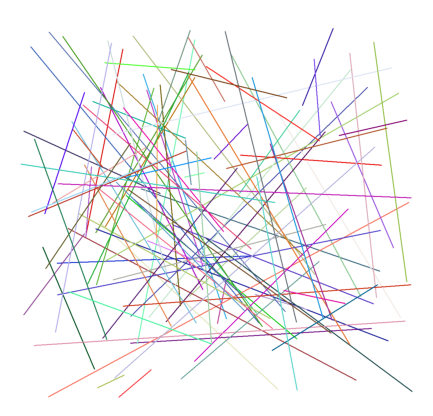
\includegraphics[keepaspectratio]{images/Visualisasi 2D dengan EMT_Isni Azizah Utami_23030630016-001.png}}
\caption{images/Visualisasi\%202D\%20dengan\%20EMT\_Isni\%20Azizah\%20Utami\_23030630016-001.png}
\end{figure}

\textgreater reset;

Anda harus menahan grafik, karena perintah plot() akan menghapus jendela plot.

Untuk menghapus semua yang telah kita lakukan, kita menggunakan reset().

Untuk menampilkan gambar hasil plot di layar notebook, perintah plot2d() dapat diakhiri dengan titik dua (:). Cara lain adalah perintah plot2d() diakhiri dengan titik koma (;), kemudian menggunakan perintah insimg() untuk menampilkan gambar hasil plot.

Sebagai contoh lain, kita menggambar plot sebagai inset dalam plot lain. Hal ini dilakukan dengan mendefinisikan jendela plot yang lebih kecil. Perhatikan bahwa jendela ini tidak menyediakan ruang untuk label sumbu di luar jendela plot. Kita harus menambahkan beberapa margin untuk hal ini sesuai kebutuhan. Perhatikan bahwa kita menyimpan dan mengembalikan jendela penuh, dan menahan plot saat ini sementara kita membuat inset.

\textgreater plot2d(``x\^{}3-x'');

\textgreater xw=200; yw=100; ww=300; hw=300;

\textgreater ow=window();

\textgreater window(xw,yw,xw+ww,yw+hw);

\textgreater hold on;

\textgreater barclear(xw-50,yw-10,ww+60,ww+60);

\textgreater plot2d(``x\^{}4-x'',grid=6):

\begin{figure}
\centering
\pandocbounded{\includegraphics[keepaspectratio]{images/Visualisasi 2D dengan EMT_Isni Azizah Utami_23030630016-002.png}}
\caption{images/Visualisasi\%202D\%20dengan\%20EMT\_Isni\%20Azizah\%20Utami\_23030630016-002.png}
\end{figure}

\textgreater hold off;

\textgreater window(ow);

Plot dengan beberapa angka dicapai dengan cara yang sama. Ada fungsi utility figure() untuk ini.

\section{Plot~Aspect}\label{plot-aspect}

Plot default menggunakan jendela plot persegi. Anda dapat mengubahnya dengan fungsi aspect(). Jangan lupa untuk mengatur ulang aspeknya nanti. Anda juga dapat mengubah default ini di menu dengan ``Set Aspect'' ke rasio aspek tertentu atau ke ukuran jendela grafis saat ini.

Tetapi Anda juga dapat mengubahnya untuk satu plot. Untuk ini, ukuran area plot saat ini diubah, dan jendela diatur sedemikian rupa sehingga label memiliki ruang yang cukup.

\textgreater aspect(2); // rasio panjang dan lebar 2:1

\textgreater plot2d({[}``sin(x)'',``cos(x)''{]},0,2pi):

\begin{figure}
\centering
\pandocbounded{\includegraphics[keepaspectratio]{images/Visualisasi 2D dengan EMT_Isni Azizah Utami_23030630016-003.png}}
\caption{images/Visualisasi\%202D\%20dengan\%20EMT\_Isni\%20Azizah\%20Utami\_23030630016-003.png}
\end{figure}

\textgreater aspect();

\textgreater reset;

Fungsi reset () mengembalikan default plot, termasuk rasio aspek.

\section{2D Plots in Euler}\label{d-plots-in-euler}

EMT Math Toolbox memiliki plot dalam bentuk 2D, baik untuk data maupun fungsi. EMT menggunakan fungsi plot2d. Fungsi ini dapat memplot fungsi dan data.

Dimungkinkan untuk memplot di Maxima menggunakan Gnuplot atau di Python menggunakan Math Plot Lib.

Euler dapat memplot plot 2D dari

\begin{itemize}
\tightlist
\item
  ekspresi
\item
  fungsi, variabel, atau kurva berparameter,
\item
  vektor nilai x-y,
\item
  awan titik-titik di bidang,
\item
  kurva implisit dengan level atau wilayah level.
\item
  Fungsi yang kompleks
\end{itemize}

Gaya plot mencakup berbagai gaya untuk garis dan titik, plot batang, dan plot berbayang.

\section{Plot Ekspresi atau Variabel}\label{plot-ekspresi-atau-variabel}

Ekspresi tunggal dalam ``x'' (misalnya ``4*x\^{}2'') atau nama fungsi (misalnya ``f'') menghasilkan grafik fungsi.

Berikut ini adalah contoh paling dasar, yang menggunakan rentang default dan menetapkan rentang y yang tepat agar sesuai dengan plot fungsi.

Catatan: Jika Anda mengakhiri baris perintah dengan tanda titik dua ``:'', plot akan disisipkan ke dalam jendela teks. Jika tidak, tekan TAB untuk melihat plot jika jendela plot tertutup.

\textgreater plot2d(``x\^{}2''):

\begin{figure}
\centering
\pandocbounded{\includegraphics[keepaspectratio]{images/Visualisasi 2D dengan EMT_Isni Azizah Utami_23030630016-004.png}}
\caption{images/Visualisasi\%202D\%20dengan\%20EMT\_Isni\%20Azizah\%20Utami\_23030630016-004.png}
\end{figure}

\textgreater aspect(1.5); plot2d(``x\^{}3-x''):

\begin{figure}
\centering
\pandocbounded{\includegraphics[keepaspectratio]{images/Visualisasi 2D dengan EMT_Isni Azizah Utami_23030630016-005.png}}
\caption{images/Visualisasi\%202D\%20dengan\%20EMT\_Isni\%20Azizah\%20Utami\_23030630016-005.png}
\end{figure}

\textgreater a:=5.6; plot2d(``exp(-a*x\^{}2)/a''); insimg(30); // menampilkan gambar hasil plot setinggi 25 baris

\begin{figure}
\centering
\pandocbounded{\includegraphics[keepaspectratio]{images/Visualisasi 2D dengan EMT_Isni Azizah Utami_23030630016-006.png}}
\caption{images/Visualisasi\%202D\%20dengan\%20EMT\_Isni\%20Azizah\%20Utami\_23030630016-006.png}
\end{figure}

Dari beberapa contoh sebelumnya Anda dapat melihat bahwa aslinya gambar plot menggunakan sumbu X dengan rentang nilai dari -2 sampai dengan 2. Untuk mengubah rentang nilai X dan Y, Anda dapat menambahkan nilai-nilai batas X (dan Y) di belakang ekspresi yang digambar.

Rentang plot ditetapkan dengan parameter yang ditetapkan berikut ini

\begin{itemize}
\tightlist
\item
  a,b: x-range (default -2,2)
\item
  c,d: y-range (default: scale with values)
\item
  r: sebagai alternatif, radius di sekitar pusat plot
\item
  cx,cy: koordinat pusat plot (default 0,0)
\end{itemize}

\textgreater plot2d(``x\^{}3-x'',-1,2):

\begin{figure}
\centering
\pandocbounded{\includegraphics[keepaspectratio]{images/Visualisasi 2D dengan EMT_Isni Azizah Utami_23030630016-007.png}}
\caption{images/Visualisasi\%202D\%20dengan\%20EMT\_Isni\%20Azizah\%20Utami\_23030630016-007.png}
\end{figure}

\textgreater plot2d(``sin(x)'',-2*pi,2*pi): // plot sin(x) pada interval {[}-2pi, 2pi{]}

\begin{figure}
\centering
\pandocbounded{\includegraphics[keepaspectratio]{images/Visualisasi 2D dengan EMT_Isni Azizah Utami_23030630016-008.png}}
\caption{images/Visualisasi\%202D\%20dengan\%20EMT\_Isni\%20Azizah\%20Utami\_23030630016-008.png}
\end{figure}

\textgreater plot2d(``cos(x)'',``sin(3*x)'',xmin=0,xmax=2pi):

\begin{figure}
\centering
\pandocbounded{\includegraphics[keepaspectratio]{images/Visualisasi 2D dengan EMT_Isni Azizah Utami_23030630016-009.png}}
\caption{images/Visualisasi\%202D\%20dengan\%20EMT\_Isni\%20Azizah\%20Utami\_23030630016-009.png}
\end{figure}

Alternatif untuk tanda titik dua adalah perintah insimg(lines), yang menyisipkan plot yang menempati sejumlah baris teks tertentu.

Dalam opsi, plot dapat diatur untuk muncul di jendela terpisah yang dapat diubah ukurannya, di jendela buku catatan. Lebih banyak gaya yang dapat dicapai dengan perintah plot tertentu.

Dalam hal apa pun, tekan tombol tabulator untuk melihat plot, jika disembunyikan.

Untuk membagi jendela menjadi beberapa plot, gunakan perintah figure(). Pada contoh, kita memplot x\^{}1 sampai x\^{}4 ke dalam 4 bagian jendela. figure(0) akan mereset jendela default.

\textgreater reset;

\textgreater figure(2,2); \ldots{}\\
\textgreater{} for n=1 to 4; figure(n); plot2d(``x\^{}''+n); end; \ldots{}\\
\textgreater{} figure(0):

\begin{figure}
\centering
\pandocbounded{\includegraphics[keepaspectratio]{images/Visualisasi 2D dengan EMT_Isni Azizah Utami_23030630016-010.png}}
\caption{images/Visualisasi\%202D\%20dengan\%20EMT\_Isni\%20Azizah\%20Utami\_23030630016-010.png}
\end{figure}

Pada plot2d(), terdapat beberapa gaya alternatif yang tersedia dengan grid=x. Sebagai gambaran umum, kami menampilkan berbagai gaya grid pada satu gambar (lihat di bawah ini untuk perintah figure()). Gaya grid=0 tidak disertakan. Gaya ini tidak menampilkan grid dan frame.

\textgreater figure(3,3); \ldots{}\\
\textgreater{} for k=1:9; figure(k); plot2d(``x\^{}3-x'',-2,1,grid=k); end; \ldots{}\\
\textgreater{} figure(0):

\begin{figure}
\centering
\pandocbounded{\includegraphics[keepaspectratio]{images/Visualisasi 2D dengan EMT_Isni Azizah Utami_23030630016-011.png}}
\caption{images/Visualisasi\%202D\%20dengan\%20EMT\_Isni\%20Azizah\%20Utami\_23030630016-011.png}
\end{figure}

Jika argumen untuk plot2d() adalah sebuah ekspresi yang diikuti oleh empat angka, angka-angka ini adalah rentang x dan y untuk plot.

Atau, a, b, c, d dapat ditentukan sebagai parameter yang ditetapkan sebagai a=\ldots{} dst.

Pada contoh berikut, kita mengubah gaya grid, menambahkan label, dan menggunakan label vertikal untuk sumbu y.

\textgreater aspect(1.5); plot2d(``sin(x)'',0,2pi,-1.2,1.2,grid=3,xl=``x'',yl=``sin(x)''):

\begin{figure}
\centering
\pandocbounded{\includegraphics[keepaspectratio]{images/Visualisasi 2D dengan EMT_Isni Azizah Utami_23030630016-012.png}}
\caption{images/Visualisasi\%202D\%20dengan\%20EMT\_Isni\%20Azizah\%20Utami\_23030630016-012.png}
\end{figure}

\textgreater plot2d(``sin(x)+cos(2*x)'',0,4pi):

\begin{figure}
\centering
\pandocbounded{\includegraphics[keepaspectratio]{images/Visualisasi 2D dengan EMT_Isni Azizah Utami_23030630016-013.png}}
\caption{images/Visualisasi\%202D\%20dengan\%20EMT\_Isni\%20Azizah\%20Utami\_23030630016-013.png}
\end{figure}

Gambar yang dihasilkan dengan menyisipkan plot ke dalam jendela teks disimpan dalam direktori yang sama dengan notebook, secara default dalam subdirektori bernama ``images''. Gambar-gambar tersebut juga digunakan oleh ekspor HTML.

Anda cukup menandai gambar mana saja dan menyalinnya ke clipboard dengan Ctrl-C. Tentu saja, Anda juga dapat mengekspor grafik saat ini dengan fungsi-fungsi pada menu File.

Fungsi atau ekspresi dalam plot2d dievaluasi secara adaptif. Untuk kecepatan yang lebih tinggi, matikan plot adaptif dengan \textless adaptive dan tentukan jumlah subinterval dengan n=\ldots{} Hal ini hanya diperlukan pada kasus-kasus yang jarang terjadi.

\textgreater plot2d(``sign(x)*exp(-x\^{}2)'',-1,1,\textless adaptive,n=10000):

\begin{figure}
\centering
\pandocbounded{\includegraphics[keepaspectratio]{images/Visualisasi 2D dengan EMT_Isni Azizah Utami_23030630016-014.png}}
\caption{images/Visualisasi\%202D\%20dengan\%20EMT\_Isni\%20Azizah\%20Utami\_23030630016-014.png}
\end{figure}

\textgreater plot2d(``x\^{}x'',r=1.2,cx=1,cy=1):

\begin{figure}
\centering
\pandocbounded{\includegraphics[keepaspectratio]{images/Visualisasi 2D dengan EMT_Isni Azizah Utami_23030630016-015.png}}
\caption{images/Visualisasi\%202D\%20dengan\%20EMT\_Isni\%20Azizah\%20Utami\_23030630016-015.png}
\end{figure}

Perhatikan bahwa x\^{}x tidak didefinisikan untuk x\textless=0. Fungsi plot2d menangkap kesalahan ini, dan mulai memplot segera setelah fungsi didefinisikan. Hal ini berlaku untuk semua fungsi yang mengembalikan NAN di luar jangkauan definisinya.

\textgreater plot2d(``log(x)'',-0.1,2):

\begin{figure}
\centering
\pandocbounded{\includegraphics[keepaspectratio]{images/Visualisasi 2D dengan EMT_Isni Azizah Utami_23030630016-016.png}}
\caption{images/Visualisasi\%202D\%20dengan\%20EMT\_Isni\%20Azizah\%20Utami\_23030630016-016.png}
\end{figure}

Parameter square=true (atau \textgreater square) memilih rentang y secara otomatis sehingga hasilnya adalah jendela plot persegi. Perhatikan bahwa secara default, Euler menggunakan ruang persegi di dalam jendela plot.

\textgreater plot2d(``x\^{}3-x'',\textgreater square):

\begin{figure}
\centering
\pandocbounded{\includegraphics[keepaspectratio]{images/Visualisasi 2D dengan EMT_Isni Azizah Utami_23030630016-017.png}}
\caption{images/Visualisasi\%202D\%20dengan\%20EMT\_Isni\%20Azizah\%20Utami\_23030630016-017.png}
\end{figure}

\textgreater plot2d(`'integrate(``sin(x)*exp(-x\^{}2)'',0,x)'\,',0,2): // plot integral

\begin{figure}
\centering
\pandocbounded{\includegraphics[keepaspectratio]{images/Visualisasi 2D dengan EMT_Isni Azizah Utami_23030630016-018.png}}
\caption{images/Visualisasi\%202D\%20dengan\%20EMT\_Isni\%20Azizah\%20Utami\_23030630016-018.png}
\end{figure}

Jika Anda membutuhkan lebih banyak ruang untuk label-y, panggil shrinkwindow() dengan parameter lebih kecil, atau tetapkan nilai positif untuk ``smaller'' pada plot2d().

\textgreater plot2d(``gamma(x)'',1,10,yl=``y-values'',smaller=6,\textless vertical):

\begin{figure}
\centering
\pandocbounded{\includegraphics[keepaspectratio]{images/Visualisasi 2D dengan EMT_Isni Azizah Utami_23030630016-019.png}}
\caption{images/Visualisasi\%202D\%20dengan\%20EMT\_Isni\%20Azizah\%20Utami\_23030630016-019.png}
\end{figure}

Ekspresi simbolik juga dapat digunakan, karena disimpan sebagai ekspresi string sederhana.

\textgreater x=linspace(0,2pi,1000); plot2d(sin(5x),cos(7x)):

\begin{figure}
\centering
\pandocbounded{\includegraphics[keepaspectratio]{images/Visualisasi 2D dengan EMT_Isni Azizah Utami_23030630016-020.png}}
\caption{images/Visualisasi\%202D\%20dengan\%20EMT\_Isni\%20Azizah\%20Utami\_23030630016-020.png}
\end{figure}

\textgreater a:=5.6; expr \&= exp(-a*x\^{}2)/a; // define expression

\textgreater plot2d(expr,-2,2): // plot from -2 to 2

\begin{figure}
\centering
\pandocbounded{\includegraphics[keepaspectratio]{images/Visualisasi 2D dengan EMT_Isni Azizah Utami_23030630016-021.png}}
\caption{images/Visualisasi\%202D\%20dengan\%20EMT\_Isni\%20Azizah\%20Utami\_23030630016-021.png}
\end{figure}

\textgreater plot2d(expr,r=1,thickness=2): // plot in a square around (0,0)

\begin{figure}
\centering
\pandocbounded{\includegraphics[keepaspectratio]{images/Visualisasi 2D dengan EMT_Isni Azizah Utami_23030630016-022.png}}
\caption{images/Visualisasi\%202D\%20dengan\%20EMT\_Isni\%20Azizah\%20Utami\_23030630016-022.png}
\end{figure}

\textgreater plot2d(\&diff(expr,x),\textgreater add,style=``--'',color=red): // add another plot

\begin{figure}
\centering
\pandocbounded{\includegraphics[keepaspectratio]{images/Visualisasi 2D dengan EMT_Isni Azizah Utami_23030630016-023.png}}
\caption{images/Visualisasi\%202D\%20dengan\%20EMT\_Isni\%20Azizah\%20Utami\_23030630016-023.png}
\end{figure}

\textgreater plot2d(\&diff(expr,x,2),a=-2,b=2,c=-2,d=1): // plot in rectangle

\begin{figure}
\centering
\pandocbounded{\includegraphics[keepaspectratio]{images/Visualisasi 2D dengan EMT_Isni Azizah Utami_23030630016-024.png}}
\caption{images/Visualisasi\%202D\%20dengan\%20EMT\_Isni\%20Azizah\%20Utami\_23030630016-024.png}
\end{figure}

\textgreater plot2d(\&diff(expr,x),a=-2,b=2,\textgreater square): // keep plot square

\begin{figure}
\centering
\pandocbounded{\includegraphics[keepaspectratio]{images/Visualisasi 2D dengan EMT_Isni Azizah Utami_23030630016-025.png}}
\caption{images/Visualisasi\%202D\%20dengan\%20EMT\_Isni\%20Azizah\%20Utami\_23030630016-025.png}
\end{figure}

\textgreater plot2d(``x\^{}2'',0,1,steps=1,color=red,n=10):

\begin{figure}
\centering
\pandocbounded{\includegraphics[keepaspectratio]{images/Visualisasi 2D dengan EMT_Isni Azizah Utami_23030630016-026.png}}
\caption{images/Visualisasi\%202D\%20dengan\%20EMT\_Isni\%20Azizah\%20Utami\_23030630016-026.png}
\end{figure}

\textgreater plot2d(``x\^{}2'',\textgreater add,steps=2,color=blue,n=10):

\begin{figure}
\centering
\pandocbounded{\includegraphics[keepaspectratio]{images/Visualisasi 2D dengan EMT_Isni Azizah Utami_23030630016-027.png}}
\caption{images/Visualisasi\%202D\%20dengan\%20EMT\_Isni\%20Azizah\%20Utami\_23030630016-027.png}
\end{figure}

\section{Functions in one Parameter}\label{functions-in-one-parameter}

Fungsi plot yang paling penting untuk plot planar adalah plot2d(). Fungsi ini diimplementasikan dalam bahasa Euler dalam file ``plot.e'', yang dimuat pada awal program.

Berikut adalah beberapa contoh penggunaan fungsi. Seperti biasa dalam EMT, fungsi yang bekerja untuk fungsi atau ekspresi lain, Anda dapat mengoper parameter tambahan (selain x) yang bukan variabel global ke fungsi dengan parameter titik koma atau dengan koleksi panggilan.

\textgreater function f(x,a) := x\textsuperscript{2/a+a*x}2-x; // define a function

\textgreater a=0.3; plot2d(``f'',0,1;a): // plot with a=0.3

\begin{figure}
\centering
\pandocbounded{\includegraphics[keepaspectratio]{images/Visualisasi 2D dengan EMT_Isni Azizah Utami_23030630016-028.png}}
\caption{images/Visualisasi\%202D\%20dengan\%20EMT\_Isni\%20Azizah\%20Utami\_23030630016-028.png}
\end{figure}

\textgreater plot2d(``f'',0,1;0.4): // plot with a=0.4

\begin{figure}
\centering
\pandocbounded{\includegraphics[keepaspectratio]{images/Visualisasi 2D dengan EMT_Isni Azizah Utami_23030630016-029.png}}
\caption{images/Visualisasi\%202D\%20dengan\%20EMT\_Isni\%20Azizah\%20Utami\_23030630016-029.png}
\end{figure}

\textgreater plot2d(\{\{``f'',0.2\}\},0,1): // plot with a=0.2

\begin{figure}
\centering
\pandocbounded{\includegraphics[keepaspectratio]{images/Visualisasi 2D dengan EMT_Isni Azizah Utami_23030630016-030.png}}
\caption{images/Visualisasi\%202D\%20dengan\%20EMT\_Isni\%20Azizah\%20Utami\_23030630016-030.png}
\end{figure}

\textgreater plot2d(\{\{``f(x,b)'',b=0.1\}\},0,1): // plot with 0.1

\begin{figure}
\centering
\pandocbounded{\includegraphics[keepaspectratio]{images/Visualisasi 2D dengan EMT_Isni Azizah Utami_23030630016-031.png}}
\caption{images/Visualisasi\%202D\%20dengan\%20EMT\_Isni\%20Azizah\%20Utami\_23030630016-031.png}
\end{figure}

\textgreater function f(x) := x\^{}3-x; \ldots{}\\
\textgreater{} plot2d(``f'',r=1):

\begin{figure}
\centering
\pandocbounded{\includegraphics[keepaspectratio]{images/Visualisasi 2D dengan EMT_Isni Azizah Utami_23030630016-032.png}}
\caption{images/Visualisasi\%202D\%20dengan\%20EMT\_Isni\%20Azizah\%20Utami\_23030630016-032.png}
\end{figure}

Berikut ini adalah ringkasan dari fungsi yang diterima

\begin{itemize}
\tightlist
\item
  ekspresi atau ekspresi simbolik dalam x
\item
  fungsi atau fungsi simbolik dengan nama sebagai ``f''
\item
  fungsi-fungsi simbolik hanya dengan nama f
\end{itemize}

Fungsi plot2d() juga menerima fungsi simbolik. Untuk fungsi simbolik, nama saja sudah cukup.

\textgreater function f(x) \&= diff(x\^{}x,x)

\begin{verbatim}
                            x
                           x  (log(x) + 1)
\end{verbatim}

\textgreater plot2d(f,0,2):

\begin{figure}
\centering
\pandocbounded{\includegraphics[keepaspectratio]{images/Visualisasi 2D dengan EMT_Isni Azizah Utami_23030630016-033.png}}
\caption{images/Visualisasi\%202D\%20dengan\%20EMT\_Isni\%20Azizah\%20Utami\_23030630016-033.png}
\end{figure}

Tentu saja, untuk ekspresi atau ungkapan simbolik, nama variabel sudah cukup untuk memplotnya.

\textgreater expr \&= sin(x)*exp(-x)

\begin{verbatim}
                              - x
                             E    sin(x)
\end{verbatim}

\textgreater plot2d(expr,0,3pi):

\begin{figure}
\centering
\pandocbounded{\includegraphics[keepaspectratio]{images/Visualisasi 2D dengan EMT_Isni Azizah Utami_23030630016-034.png}}
\caption{images/Visualisasi\%202D\%20dengan\%20EMT\_Isni\%20Azizah\%20Utami\_23030630016-034.png}
\end{figure}

\textgreater function f(x) \&= x\^{}x;

\textgreater plot2d(f,r=1,cx=1,cy=1,color=blue,thickness=2);

\textgreater plot2d(\&diff(f(x),x),\textgreater add,color=red,style=``-.-''):

\begin{figure}
\centering
\pandocbounded{\includegraphics[keepaspectratio]{images/Visualisasi 2D dengan EMT_Isni Azizah Utami_23030630016-035.png}}
\caption{images/Visualisasi\%202D\%20dengan\%20EMT\_Isni\%20Azizah\%20Utami\_23030630016-035.png}
\end{figure}

\textgreater function f:= (a*(x\^{}2/a))

\textgreater plot2d(f,a=4)

Untuk gaya garis, ada berbagai pilihan.

\begin{itemize}
\tightlist
\item
  style=``\ldots{}''. pilih dari''-``,''--``,''-.'', ``.'', ``.-.'', ``-.-''.
\item
  color: lihat dibawah untuk warna
\item
  thickness: Defaultnya adalah 1.
\end{itemize}

Warna dapat dipilih sebagai salah satu warna default, atau sebagai warna RGB.

\begin{itemize}
\tightlist
\item
  0..15: indeks warna default.
\item
  color constants: white, black, red, green, blue, cyan, olive,
\item
  lightgray, gray, darkgray, orange, lightgreen, turquoise, lightblue, lightorange, yellow
\item
  rgb(red,green,blue): parameters are reals in {[}0,1{]}.
\end{itemize}

\textgreater plot2d(``exp(-x\^{}2)'',r=2,color=red,thickness=3,style=``--''):

\begin{figure}
\centering
\pandocbounded{\includegraphics[keepaspectratio]{images/Visualisasi 2D dengan EMT_Isni Azizah Utami_23030630016-036.png}}
\caption{images/Visualisasi\%202D\%20dengan\%20EMT\_Isni\%20Azizah\%20Utami\_23030630016-036.png}
\end{figure}

Berikut ini adalah pemandangan warna EMT yang sudah ditetapkan sebelumnya.

\textgreater aspect(2); columnsplot(ones(1,16),lab=0:15,grid=0,color=0:15):

\begin{figure}
\centering
\pandocbounded{\includegraphics[keepaspectratio]{images/Visualisasi 2D dengan EMT_Isni Azizah Utami_23030630016-037.png}}
\caption{images/Visualisasi\%202D\%20dengan\%20EMT\_Isni\%20Azizah\%20Utami\_23030630016-037.png}
\end{figure}

Tetapi anda dapat menggunakan warna apapun.

\textgreater columnsplot(ones(1,16),grid=0,color=rgb(0,0,linspace(0,1,15))):

\begin{figure}
\centering
\pandocbounded{\includegraphics[keepaspectratio]{images/Visualisasi 2D dengan EMT_Isni Azizah Utami_23030630016-038.png}}
\caption{images/Visualisasi\%202D\%20dengan\%20EMT\_Isni\%20Azizah\%20Utami\_23030630016-038.png}
\end{figure}

\section{Menggambar Beberapa Kurva pada bidang koordinat yang sama}\label{menggambar-beberapa-kurva-pada-bidang-koordinat-yang-sama}

Memplot lebih dari satu fungsi (beberapa fungsi) ke dalam satu jendela dapat dilakukan dengan berbagai cara. Salah satu caranya adalah dengan menggunakan \textgreater add untuk beberapa pemanggilan ke plot2d secara bersamaan, kecuali pemanggilan pertama. Kita telah menggunakan fitur ini pada contoh di atas.

\textgreater aspect(); plot2d(``cos(x)'',r=2,grid=6); plot2d(``x'',style=``.'',\textgreater add):

\begin{figure}
\centering
\pandocbounded{\includegraphics[keepaspectratio]{images/Visualisasi 2D dengan EMT_Isni Azizah Utami_23030630016-039.png}}
\caption{images/Visualisasi\%202D\%20dengan\%20EMT\_Isni\%20Azizah\%20Utami\_23030630016-039.png}
\end{figure}

\textgreater aspect(1.5); plot2d(``sin(x)'',0,2pi); plot2d(``cos(x)'',color=blue,style=``--'',\textgreater add):

\begin{figure}
\centering
\pandocbounded{\includegraphics[keepaspectratio]{images/Visualisasi 2D dengan EMT_Isni Azizah Utami_23030630016-040.png}}
\caption{images/Visualisasi\%202D\%20dengan\%20EMT\_Isni\%20Azizah\%20Utami\_23030630016-040.png}
\end{figure}

Salah satu kegunaan \textgreater add adalah untuk menambahkan titik pada kurva.

\textgreater plot2d(``sin(x)'',0,pi); plot2d(2,sin(2),\textgreater points,\textgreater add):

\begin{figure}
\centering
\pandocbounded{\includegraphics[keepaspectratio]{images/Visualisasi 2D dengan EMT_Isni Azizah Utami_23030630016-041.png}}
\caption{images/Visualisasi\%202D\%20dengan\%20EMT\_Isni\%20Azizah\%20Utami\_23030630016-041.png}
\end{figure}

Kami menambahkan titik perpotongan dengan label (pada posisi ``cl'' untuk kiri tengah), dan menyisipkan hasilnya ke dalam buku catatan. Kami juga menambahkan judul ke plot.

\textgreater plot2d({[}``cos(x)'',``x''{]},r=1.1,cx=0.5,cy=0.5, \ldots{}\\
\textgreater{} color={[}black,blue{]},style={[}``-'',``.''{]}, \ldots{}\\
\textgreater{} grid=1);

\textgreater x0=solve(``cos(x)-x'',1); \ldots{}\\
\textgreater{} plot2d(x0,x0,\textgreater points,\textgreater add,title=``Intersection Demo''); \ldots{}\\
\textgreater{} label(``cos(x) = x'',x0,x0,pos=``cl'',offset=20):

\begin{figure}
\centering
\pandocbounded{\includegraphics[keepaspectratio]{images/Visualisasi 2D dengan EMT_Isni Azizah Utami_23030630016-042.png}}
\caption{images/Visualisasi\%202D\%20dengan\%20EMT\_Isni\%20Azizah\%20Utami\_23030630016-042.png}
\end{figure}

Dalam demo berikut ini, kami memplot fungsi sinc(x)=sin(x)/x dan ekspansi Taylor ke-8 dan ke-16. Kami menghitung ekspansi ini menggunakan Maxima melalui ekspresi simbolik.

Plot ini dilakukan dalam perintah multi-baris berikut dengan tiga pemanggilan plot2d(). Perintah kedua dan ketiga memiliki set flag \textgreater add, yang membuat plot menggunakan rentang sebelumnya.

Kami menambahkan sebuah kotak label yang menjelaskan fungsi-fungsi tersebut.

\textgreater{}\(taylor(sin(x)/x,x,0,4)\)\(\frac{x^4}{120}-\frac{x^2}{6}+1\)\$\textgreater plot2d(``sinc(x)'',0,4pi,color=green,thickness=2); \ldots{}\\
\textgreater{} plot2d(\&taylor(sin(x)/x,x,0,8),\textgreater add,color=blue,style=``--''); \ldots{}\\
\textgreater{} plot2d(\&taylor(sin(x)/x,x,0,16),\textgreater add,color=red,style=``-.-''); \ldots{}\\
\textgreater{} labelbox({[}``sinc'',``T8'',``T16''{]},styles={[}``-'',``--'',``-.-''{]}, \ldots{}\\
\textgreater{} colors={[}black,blue,red{]}):

\begin{figure}
\centering
\pandocbounded{\includegraphics[keepaspectratio]{images/Visualisasi 2D dengan EMT_Isni Azizah Utami_23030630016-044.png}}
\caption{images/Visualisasi\%202D\%20dengan\%20EMT\_Isni\%20Azizah\%20Utami\_23030630016-044.png}
\end{figure}

Pada contoh berikut, kami menghasilkan Polinomial Bernstein.

\textgreater plot2d(``(1-x)\^{}10'',0,1); // plot first function

\textgreater for i=1 to 10; plot2d(``bin(10,i)*x\textsuperscript{i*(1-x)}(10-i)'',\textgreater add); end;

\textgreater insimg;

\begin{figure}
\centering
\pandocbounded{\includegraphics[keepaspectratio]{images/Visualisasi 2D dengan EMT_Isni Azizah Utami_23030630016-045.png}}
\caption{images/Visualisasi\%202D\%20dengan\%20EMT\_Isni\%20Azizah\%20Utami\_23030630016-045.png}
\end{figure}

Metode kedua menggunakan sepasang matriks nilai x dan matriks nilai y dengan ukuran yang sama.

Kita membuat sebuah matriks nilai dengan satu Polinomial Bernstein di setiap baris. Untuk ini, kita cukup menggunakan vektor kolom i. Lihatlah pengantar tentang bahasa matriks untuk mempelajari lebih lanjut.

\textgreater x=linspace(0,1,500);

\textgreater n=10; k=(0:n)'; // n is row vector, k is column vector

\textgreater y=bin(n,k)*x\textsuperscript{k*(1-x)}(n-k); // y is a matrix then

\textgreater plot2d(x,y):

\begin{figure}
\centering
\pandocbounded{\includegraphics[keepaspectratio]{images/Visualisasi 2D dengan EMT_Isni Azizah Utami_23030630016-046.png}}
\caption{images/Visualisasi\%202D\%20dengan\%20EMT\_Isni\%20Azizah\%20Utami\_23030630016-046.png}
\end{figure}

Perhatikan bahwa parameter warna dapat berupa vektor. Kemudian setiap warna digunakan untuk setiap baris matriks.

\textgreater x=linspace(0,1,200); y=x\^{}(1:10)'; plot2d(x,y,color=1:10):

\begin{figure}
\centering
\pandocbounded{\includegraphics[keepaspectratio]{images/Visualisasi 2D dengan EMT_Isni Azizah Utami_23030630016-047.png}}
\caption{images/Visualisasi\%202D\%20dengan\%20EMT\_Isni\%20Azizah\%20Utami\_23030630016-047.png}
\end{figure}

Metode lainnya adalah menggunakan vektor ekspresi (string). Anda kemudian dapat menggunakan larik warna, larik gaya, dan larik ketebalan dengan panjang yang sama.

\textgreater plot2d({[}``sin(x)'',``cos(x)''{]},0,2pi,color=4:5):

\begin{figure}
\centering
\pandocbounded{\includegraphics[keepaspectratio]{images/Visualisasi 2D dengan EMT_Isni Azizah Utami_23030630016-048.png}}
\caption{images/Visualisasi\%202D\%20dengan\%20EMT\_Isni\%20Azizah\%20Utami\_23030630016-048.png}
\end{figure}

\textgreater plot2d({[}``sin(x)'',``cos(x)''{]},0,2pi): // plot vector of expressions

\begin{figure}
\centering
\pandocbounded{\includegraphics[keepaspectratio]{images/Visualisasi 2D dengan EMT_Isni Azizah Utami_23030630016-049.png}}
\caption{images/Visualisasi\%202D\%20dengan\%20EMT\_Isni\%20Azizah\%20Utami\_23030630016-049.png}
\end{figure}

Kita bisa mendapatkan vektor seperti itu dari Maxima dengan menggunakan makelist() dan mxm2str().

\textgreater v \&= makelist(binomial(10,i)*x\textsuperscript{i*(1-x)}(10-i),i,0,10) // make list

\begin{verbatim}
               10            9              8  2             7  3
       [(1 - x)  , 10 (1 - x)  x, 45 (1 - x)  x , 120 (1 - x)  x , 
           6  4             5  5             4  6             3  7
210 (1 - x)  x , 252 (1 - x)  x , 210 (1 - x)  x , 120 (1 - x)  x , 
          2  8              9   10
45 (1 - x)  x , 10 (1 - x) x , x  ]
\end{verbatim}

\textgreater mxm2str(v) // get a vector of strings from the symbolic vector

\begin{verbatim}
(1-x)^10
10*(1-x)^9*x
45*(1-x)^8*x^2
120*(1-x)^7*x^3
210*(1-x)^6*x^4
252*(1-x)^5*x^5
210*(1-x)^4*x^6
120*(1-x)^3*x^7
45*(1-x)^2*x^8
10*(1-x)*x^9
x^10
\end{verbatim}

\textgreater plot2d(mxm2str(v),0,1): // plot functions

\begin{figure}
\centering
\pandocbounded{\includegraphics[keepaspectratio]{images/Visualisasi 2D dengan EMT_Isni Azizah Utami_23030630016-050.png}}
\caption{images/Visualisasi\%202D\%20dengan\%20EMT\_Isni\%20Azizah\%20Utami\_23030630016-050.png}
\end{figure}

Alternatif lain adalah dengan menggunakan bahasa matriks Euler.

Jika sebuah ekspresi menghasilkan sebuah matriks fungsi, dengan satu fungsi di setiap baris, semua fungsi ini akan diplot ke dalam satu plot.

Untuk ini, gunakan vektor parameter dalam bentuk vektor kolom. Jika sebuah larik warna ditambahkan, maka akan digunakan untuk setiap baris plot.

\textgreater n=(1:10)'; plot2d(``x\^{}n'',0,1,color=1:10):

\begin{figure}
\centering
\pandocbounded{\includegraphics[keepaspectratio]{images/Visualisasi 2D dengan EMT_Isni Azizah Utami_23030630016-051.png}}
\caption{images/Visualisasi\%202D\%20dengan\%20EMT\_Isni\%20Azizah\%20Utami\_23030630016-051.png}
\end{figure}

Ekspresi dan fungsi satu baris dapat melihat variabel global.

Jika Anda tidak dapat menggunakan variabel global, Anda perlu menggunakan fungsi dengan parameter tambahan, dan memberikan parameter ini sebagai parameter titik koma.

Berhati-hatilah untuk meletakkan semua parameter yang diberikan di akhir perintah plot2d. Pada contoh ini kita mengoper a=5 ke fungsi f, yang kita plot dari -10 ke 10.

\textgreater function f(x,a) := 1/a*exp(-x\^{}2/a); \ldots{}\\
\textgreater{} plot2d(``f'',-10,10;5,thickness=2,title=``a=5''):

\begin{figure}
\centering
\pandocbounded{\includegraphics[keepaspectratio]{images/Visualisasi 2D dengan EMT_Isni Azizah Utami_23030630016-052.png}}
\caption{images/Visualisasi\%202D\%20dengan\%20EMT\_Isni\%20Azizah\%20Utami\_23030630016-052.png}
\end{figure}

Atau, gunakan koleksi dengan nama fungsi dan semua parameter tambahan. Daftar khusus ini disebut koleksi panggilan, dan itu adalah cara yang lebih disukai untuk mengoper argumen ke fungsi yang dengan sendirinya dioper sebagai argumen ke fungsi lain.

Pada contoh berikut, kita menggunakan perulangan untuk memplot beberapa fungsi (lihat tutorial tentang pemrograman perulangan).

\textgreater plot2d(\{\{``f'',1\}\},-10,10); \ldots{}\\
\textgreater{} for a=2:10; plot2d(\{\{``f'',a\}\},\textgreater add); end:

\begin{figure}
\centering
\pandocbounded{\includegraphics[keepaspectratio]{images/Visualisasi 2D dengan EMT_Isni Azizah Utami_23030630016-053.png}}
\caption{images/Visualisasi\%202D\%20dengan\%20EMT\_Isni\%20Azizah\%20Utami\_23030630016-053.png}
\end{figure}

Kita dapat mencapai hasil yang sama dengan cara berikut menggunakan bahasa matriks EMT. Setiap baris dari matriks f(x,a) adalah satu fungsi. Selain itu, kita dapat mengatur warna untuk setiap baris matriks. Klik dua kali pada fungsi getspectral() untuk penjelasannya.

\textgreater x=-10:0.01:10; a=(1:10)'; plot2d(x,f(x,a),color=getspectral(a/10)):

\begin{figure}
\centering
\pandocbounded{\includegraphics[keepaspectratio]{images/Visualisasi 2D dengan EMT_Isni Azizah Utami_23030630016-054.png}}
\caption{images/Visualisasi\%202D\%20dengan\%20EMT\_Isni\%20Azizah\%20Utami\_23030630016-054.png}
\end{figure}

\section{Text Labels}\label{text-labels}

Dekorasi sederhana dapat berupa

\begin{itemize}
\tightlist
\item
  sebuah judul dengan title=``\ldots{}''
\item
  label x- and y- dengan xl=``\ldots{}'', yl=``\ldots{}''
\item
  text label yang lain dengan label(``\ldots{}'',x,y)
\end{itemize}

Perintah label akan memplotkan ke dalam plot saat ini pada koordinat plot (x,y). Perintah ini dapat menerima sebuah argumen posisi.

\textgreater plot2d(``x\textsuperscript{3-x'',-1,2,title=''y=x}3-x'',yl=``y'',xl=``x''):

\begin{figure}
\centering
\pandocbounded{\includegraphics[keepaspectratio]{images/Visualisasi 2D dengan EMT_Isni Azizah Utami_23030630016-055.png}}
\caption{images/Visualisasi\%202D\%20dengan\%20EMT\_Isni\%20Azizah\%20Utami\_23030630016-055.png}
\end{figure}

\textgreater expr := ``log(x)/x''; \ldots{}\\
\textgreater{} plot2d(expr,0.5,5,title=``y=''+expr,xl=``x'',yl=``y''); \ldots{}\\
\textgreater{} label(``(1,0)'',1,0); label(``Max'',E,expr(E),pos=``lc''):

\begin{figure}
\centering
\pandocbounded{\includegraphics[keepaspectratio]{images/Visualisasi 2D dengan EMT_Isni Azizah Utami_23030630016-056.png}}
\caption{images/Visualisasi\%202D\%20dengan\%20EMT\_Isni\%20Azizah\%20Utami\_23030630016-056.png}
\end{figure}

Ada juga fungsi labelbox(), yang dapat menampilkan fungsi dan teks. Fungsi ini membutuhkan vektor string dan warna, satu item untuk setiap fungsi.

\textgreater function f(x) \&= x\textsuperscript{2*exp(-x}2); \ldots{}\\
\textgreater{} plot2d(\&f(x),a=-3,b=3,c=-1,d=1); \ldots{}\\
\textgreater{} plot2d(\&diff(f(x),x),\textgreater add,color=blue,style=``--''); \ldots{}\\
\textgreater{} labelbox({[}``function'',``derivative''{]},styles={[}``-'',``--''{]}, \ldots{}\\
\textgreater{} colors={[}black,blue{]},w=0.4):

\begin{figure}
\centering
\pandocbounded{\includegraphics[keepaspectratio]{images/Visualisasi 2D dengan EMT_Isni Azizah Utami_23030630016-057.png}}
\caption{images/Visualisasi\%202D\%20dengan\%20EMT\_Isni\%20Azizah\%20Utami\_23030630016-057.png}
\end{figure}

Kotak tersebut berlabuh di kanan atas secara default, tetapi \textgreater left menambatkannya di kiri atas. Anda dapat memindahkannya ke tempat mana pun yang Anda suka. Posisi jangkar adalah sudut kanan atas kotak, dan angkanya adalah pecahan dari ukuran jendela grafik. Lebarnya otomatis.

Untuk plot titik, kotak label juga dapat digunakan. Tambahkan parameter \textgreater points, atau vektor bendera, satu untuk setiap label.

Pada contoh berikut, hanya ada satu fungsi. Jadi kita dapat menggunakan string sebagai pengganti vektor string. Kita mengatur warna teks menjadi hitam untuk contoh ini.

\textgreater n=10; plot2d(0:n,bin(n,0:n),\textgreater addpoints); \ldots{}\\
\textgreater{} labelbox(``Binomials'',styles=``{[}{]}'',\textgreater points,x=0.1,y=0.1, \ldots{}\\
\textgreater{} tcolor=black,\textgreater left):

\begin{figure}
\centering
\pandocbounded{\includegraphics[keepaspectratio]{images/Visualisasi 2D dengan EMT_Isni Azizah Utami_23030630016-058.png}}
\caption{images/Visualisasi\%202D\%20dengan\%20EMT\_Isni\%20Azizah\%20Utami\_23030630016-058.png}
\end{figure}

Gaya plot ini juga tersedia di statplot(). Seperti pada plot2d() warna dapat diatur untuk setiap baris plot. Terdapat lebih banyak plot khusus untuk keperluan statistik (lihat tutorial tentang statistik).

\textgreater statplot(1:10,random(2,10),color={[}red,blue{]}):

\begin{figure}
\centering
\pandocbounded{\includegraphics[keepaspectratio]{images/Visualisasi 2D dengan EMT_Isni Azizah Utami_23030630016-059.png}}
\caption{images/Visualisasi\%202D\%20dengan\%20EMT\_Isni\%20Azizah\%20Utami\_23030630016-059.png}
\end{figure}

Fitur yang serupa adalah fungsi textbox().

Lebarnya secara default adalah lebar maksimal baris teks. Tetapi bisa juga diatur oleh pengguna.

\textgreater function f(x) \&= exp(-x)*sin(2*pi*x); \ldots{}\\
\textgreater{} plot2d(``f(x)'',0,2pi); \ldots{}\\
\textgreater{} textbox(latex(``\textbackslash text\{Example of a damped oscillation\}\textbackslash{} f(x)=e\^{}\{-x\}sin(2\textbackslash pi x)''),w=0.85):

\begin{figure}
\centering
\pandocbounded{\includegraphics[keepaspectratio]{images/Visualisasi 2D dengan EMT_Isni Azizah Utami_23030630016-060.png}}
\caption{images/Visualisasi\%202D\%20dengan\%20EMT\_Isni\%20Azizah\%20Utami\_23030630016-060.png}
\end{figure}

Label teks, judul, kotak label, dan teks lainnya dapat berisi string Unicode (lihat sintaks EMT untuk mengetahui lebih lanjut tentang string Unicode).

\textgreater plot2d(``x\^{}3-x'',title=u''x → x³ - x''):

\begin{figure}
\centering
\pandocbounded{\includegraphics[keepaspectratio]{images/Visualisasi 2D dengan EMT_Isni Azizah Utami_23030630016-061.png}}
\caption{images/Visualisasi\%202D\%20dengan\%20EMT\_Isni\%20Azizah\%20Utami\_23030630016-061.png}
\end{figure}

Label pada sumbu x dan y bisa vertikal, begitu juga dengan sumbu.

\textgreater plot2d(``sinc(x)'',0,2pi,xl=``x'',yl=u''x → sinc(x)``,\textgreater vertical):

\begin{figure}
\centering
\pandocbounded{\includegraphics[keepaspectratio]{images/Visualisasi 2D dengan EMT_Isni Azizah Utami_23030630016-062.png}}
\caption{images/Visualisasi\%202D\%20dengan\%20EMT\_Isni\%20Azizah\%20Utami\_23030630016-062.png}
\end{figure}

\section{LaTeX}\label{latex}

Anda juga dapat memplot formula LaTeX jika Anda telah menginstal sistem LaTeX. Saya merekomendasikan MiKTeX. Jalur ke binari ``lateks'' dan ``dvipng'' harus berada di jalur sistem, atau Anda harus mengatur LaTeX di menu opsi.

Perhatikan, bahwa penguraian LaTeX berjalan lambat. Jika Anda ingin menggunakan LaTeX dalam plot animasi, Anda harus memanggil latex() sebelum perulangan satu kali dan menggunakan hasilnya (gambar dalam matriks RGB).

Pada plot berikut ini, kita menggunakan LaTeX untuk label x dan y, sebuah label, kotak label dan judul plot.

\textgreater plot2d(``exp(-x)*sin(x)/x'',a=0,b=2pi,c=0,d=1,grid=6,color=blue, \ldots{}\\
\textgreater{} title=latex(``\textbackslash text\{Function \(\\Phi\)\}''), \ldots{}\\
\textgreater{} xl=latex(``\textbackslash phi''),yl=latex(``\textbackslash Phi(\textbackslash phi)'')); \ldots{}\\
\textgreater{} textbox( \ldots{}\\
\textgreater{} latex(``\textbackslash Phi(\textbackslash phi) = e\^{}\{-\textbackslash phi\} \textbackslash frac\{\textbackslash sin(\textbackslash phi)\}\{\textbackslash phi\}''),x=0.8,y=0.5); \ldots{}\\
\textgreater{} label(latex(``\textbackslash Phi'',color=blue),1,0.4):

\begin{figure}
\centering
\pandocbounded{\includegraphics[keepaspectratio]{images/Visualisasi 2D dengan EMT_Isni Azizah Utami_23030630016-063.png}}
\caption{images/Visualisasi\%202D\%20dengan\%20EMT\_Isni\%20Azizah\%20Utami\_23030630016-063.png}
\end{figure}

Seringkali, kita menginginkan spasi dan label teks yang tidak sesuai pada sumbu x. Kita dapat menggunakan xaxis() dan yaxis() seperti yang akan kita tunjukkan nanti.

Cara termudah adalah dengan membuat plot kosong dengan sebuah frame menggunakan grid=4, dan kemudian menambahkan grid dengan ygrid() dan xgrid(). Pada contoh berikut, kita menggunakan tiga buah string LaTeX untuk label pada sumbu x dengan xtick().

\textgreater plot2d(``sinc(x)'',0,2pi,grid=4,\textless ticks); \ldots{}\\
\textgreater{} ygrid(-2:0.5:2,grid=6); \ldots{}\\
\textgreater{} xgrid({[}0:2{]}*pi,\textless ticks,grid=6); \ldots{}\\
\textgreater{} xtick({[}0,pi,2pi{]},{[}``0'',``\textbackslash pi'',``2\textbackslash pi''{]},\textgreater latex):

\begin{figure}
\centering
\pandocbounded{\includegraphics[keepaspectratio]{images/Visualisasi 2D dengan EMT_Isni Azizah Utami_23030630016-064.png}}
\caption{images/Visualisasi\%202D\%20dengan\%20EMT\_Isni\%20Azizah\%20Utami\_23030630016-064.png}
\end{figure}

Tentu saja, fungsi juga dapat digunakan.

\textgreater function map f(x) \ldots{}

\begin{verbatim}
if x>0 then return x^4
else return x^2
endif
endfunction
\end{verbatim}

Parameter ``map'' membantu menggunakan fungsi untuk vektor. Untuk plot, hal ini tidak diperlukan. Tetapi untuk menunjukkan bahwa vektorisasi berguna, kami menambahkan beberapa titik kunci pada plot pada x=-1, x=0 dan x=1.

Pada plot berikut, kita juga memasukkan beberapa kode LaTeX. Kami menggunakannya untuk dua label dan sebuah kotak teks. Tentu saja, Anda hanya dapat menggunakanLaTeX jika Anda telah menginstal LaTeX dengan benar.

\textgreater plot2d(``f'',-1,1,xl=``x'',yl=``f(x)'',grid=6); \ldots{}\\
\textgreater{} plot2d({[}-1,0,1{]},f({[}-1,0,1{]}),\textgreater points,\textgreater add); \ldots{}\\
\textgreater{} label(latex(``x\^{}3''),0.72,f(0.72)); \ldots{}\\
\textgreater{} label(latex(``x\^{}2''),-0.52,f(-0.52),pos=``ll''); \ldots{}\\
\textgreater{} textbox( \ldots{}\\
\textgreater{} latex(``f(x)=\textbackslash begin\{cases\} x\^{}3 \& x\textgreater0 \textbackslash\textbackslash{} x\^{}2 \& x \textbackslash le 0\textbackslash end\{cases\}''), \ldots{}\\
\textgreater{} x=0.7,y=0.2):

\begin{figure}
\centering
\pandocbounded{\includegraphics[keepaspectratio]{images/Visualisasi 2D dengan EMT_Isni Azizah Utami_23030630016-065.png}}
\caption{images/Visualisasi\%202D\%20dengan\%20EMT\_Isni\%20Azizah\%20Utami\_23030630016-065.png}
\end{figure}

\section{User Interaction}\label{user-interaction}

Ketika memplot fungsi atau ekspresi, parameter \textgreater user memungkinkan pengguna untuk memperbesar dan menggeser plot dengan tombol kursor atau mouse. Pengguna dapat

\begin{itemize}
\tightlist
\item
  memperbesar dengan + or -
\item
  memindahkan plot dengan tombol kursor
\item
  memilih jendela plot dengan mouse
\item
  mengatur ulang tampilan dengan spasi
\item
  keluar dengan return
\item
  Tombol spasi akan mengatur ulang plot ke jendela plot awal.
\item
  Ketika memplot data, bendera \textgreater user hanya akan menunggu penekanan tombol.
\end{itemize}

\textgreater plot2d(\{\{``x\^{}3-a*x'',a=1\}\},\textgreater user,title=``Press any key!''):

\begin{figure}
\centering
\pandocbounded{\includegraphics[keepaspectratio]{images/Visualisasi 2D dengan EMT_Isni Azizah Utami_23030630016-066.png}}
\caption{images/Visualisasi\%202D\%20dengan\%20EMT\_Isni\%20Azizah\%20Utami\_23030630016-066.png}
\end{figure}

\textgreater plot2d(``exp(x)*sin(x)'',user=true, \ldots{}\\
\textgreater{} title=``+/- or cursor keys (return to exit)''):

\begin{figure}
\centering
\pandocbounded{\includegraphics[keepaspectratio]{images/Visualisasi 2D dengan EMT_Isni Azizah Utami_23030630016-067.png}}
\caption{images/Visualisasi\%202D\%20dengan\%20EMT\_Isni\%20Azizah\%20Utami\_23030630016-067.png}
\end{figure}

Berikut ini menunjukkan cara interaksi pengguna tingkat lanjut (lihat tutorial tentang pemrograman untuk detailnya).

Fungsi bawaan mousedrag() menunggu peristiwa mouse atau keyboard. Fungsi ini melaporkan mouse ke bawah, mouse bergerak atau mouse ke atas, dan penekanan tombol. Fungsi dragpoints() memanfaatkan hal ini, dan mengizinkan pengguna untuk menyeret titik manapun di dalam plot.

Kita membutuhkan fungsi plot terlebih dahulu. Sebagai contoh, kita melakukan interpolasi pada 5 titik dengan sebuah polinomial. Fungsi ini harus memplot ke dalam area plot yang tetap.

\textgreater function plotf(xp,yp,select) \ldots{}

\begin{verbatim}
  d=interp(xp,yp);
  plot2d("interpval(xp,d,x)";d,xp,r=2);
  plot2d(xp,yp,>points,>add);
  if select>0 then
    plot2d(xp[select],yp[select],color=red,>points,>add);
  endif;
  title("Drag one point, or press space or return!");
endfunction
\end{verbatim}

Perhatikan parameter titik koma pada plot2d (d dan xp), yang diteruskan ke evaluasi fungsi interp(). Tanpa ini, kita harus menulis fungsi plotinterp() terlebih dahulu, untuk mengakses nilai secara global.

Sekarang kita menghasilkan beberapa nilai acak, dan membiarkan pengguna menyeret titik-titiknya.

\textgreater t=-1:0.5:1; dragpoints(``plotf'',t,random(size(t))-0.5):

\begin{figure}
\centering
\pandocbounded{\includegraphics[keepaspectratio]{images/Visualisasi 2D dengan EMT_Isni Azizah Utami_23030630016-068.png}}
\caption{images/Visualisasi\%202D\%20dengan\%20EMT\_Isni\%20Azizah\%20Utami\_23030630016-068.png}
\end{figure}

Ada juga fungsi yang memplot fungsi lain tergantung pada vektor parameter, dan memungkinkan pengguna menyesuaikan parameter ini.

Pertama, kita memerlukan fungsi plot.

\textgreater function plotf({[}a,b{]}) := plot2d(``exp(a*x)*cos(2pi*b*x)'',0,2pi;a,b);

Kemudian kita membutuhkan nama untuk parameter, nilai awal dan matriks rentang nx2, dan secara opsional, sebuah garis judul.

Terdapat slider interaktif, yang dapat mengatur nilai oleh pengguna. Fungsi dragvalues() menyediakan ini.

\textgreater dragvalues(``plotf'',{[}``a'',``b''{]},{[}-1,2{]},{[}{[}-2,2{]};{[}1,10{]}{]}, \ldots{}\\
\textgreater{} heading=``Drag these values:'',hcolor=black):

\begin{figure}
\centering
\pandocbounded{\includegraphics[keepaspectratio]{images/Visualisasi 2D dengan EMT_Isni Azizah Utami_23030630016-069.png}}
\caption{images/Visualisasi\%202D\%20dengan\%20EMT\_Isni\%20Azizah\%20Utami\_23030630016-069.png}
\end{figure}

Anda dapat membatasi nilai yang diseret menjadi bilangan bulat. Sebagai contoh, kita menulis fungsi plot, yang memplot polinomial Taylor dengan derajat n ke fungsi kosinus.

\textgreater function plotf(n) \ldots{}

\begin{verbatim}
plot2d("cos(x)",0,2pi,>square,grid=6);
plot2d(&"taylor(cos(x),x,0,@n)",color=blue,>add);
textbox("Taylor polynomial of degree "+n,0.1,0.02,style="t",>left);
endfunction
\end{verbatim}

Sekarang kita membiarkan derajat n bervariasi dari 0 sampai 20 dalam 20 stop. Hasil dari dragvalues() digunakan untuk memplot sketsa dengan n ini, dan untuk menyisipkan plot ke dalam buku catatan.

\textgreater nd=dragvalues(``plotf'',``degree'',2,{[}0,20{]},20,y=0.8, \ldots{}\\
\textgreater{} heading=``Drag the value:''); \ldots{}\\
\textgreater{} plotf(nd):

\begin{figure}
\centering
\pandocbounded{\includegraphics[keepaspectratio]{images/Visualisasi 2D dengan EMT_Isni Azizah Utami_23030630016-070.png}}
\caption{images/Visualisasi\%202D\%20dengan\%20EMT\_Isni\%20Azizah\%20Utami\_23030630016-070.png}
\end{figure}

Berikut ini adalah peragaan sederhana dari fungsi ini. Pengguna dapat menggambar di atas jendela plot, meninggalkan jejak titik.

\textgreater function dragtest \ldots{}

\begin{verbatim}
  plot2d(none,r=1,title="Drag with the mouse, or press any key!");
  start=0;
  repeat
    {flag,m,time}=mousedrag();
    if flag==0 then return; endif;
    if flag==2 then
      hold on; mark(m[1],m[2]); hold off;
    endif;
  end
endfunction
\end{verbatim}

\textgreater dragtest // lihat hasilnya dan cobalah lakukan!

\section{Styles~of~2D~Plots}\label{styles-of-2d-plots}

Secara default, EMt menghitung penanda kecil sumbu otomatis dan menambahkan label ke setiap penanda. Ini dapat diubah. Selain, itu, label dan judul dapat ditambahkan secara manual. Untuk menyetel ulang ke gaya default, gunakan reset ().

\textgreater aspect();

\textgreater figure(3,4); \ldots{}\\
\textgreater{} figure(1); plot2d(``x\^{}3-x'',grid=0); \ldots{} // no grid, frame or axis

\textgreater{} figure(2); plot2d(``x\^{}3-x'',grid=1); \ldots{} // x-y-axis

\textgreater{} figure(3); plot2d(``x\^{}3-x'',grid=2); \ldots{} // default ticks

\textgreater{} figure(4); plot2d(``x\^{}3-x'',grid=3); \ldots{} // x-y- axis with labels inside

\textgreater{} figure(5); plot2d(``x\^{}3-x'',grid=4); \ldots{} // no ticks, only labels

\textgreater{} figure(6); plot2d(``x\^{}3-x'',grid=5); \ldots{} // default, but no margin

\textgreater{} figure(7); plot2d(``x\^{}3-x'',grid=6); \ldots{} // axes only

\textgreater{} figure(8); plot2d(``x\^{}3-x'',grid=7); \ldots{} // axes only, ticks at axis

\textgreater{} figure(9); plot2d(``x\^{}3-x'',grid=8); \ldots{} // axes only, finer ticks at axis

\textgreater{} figure(10); plot2d(``x\^{}3-x'',grid=9); \ldots{} // default, small ticks inside

\textgreater{} figure(11); plot2d(``x\^{}3-x'',grid=10); \ldots// no ticks, axes only

\textgreater{} figure(0):

\begin{figure}
\centering
\pandocbounded{\includegraphics[keepaspectratio]{images/Visualisasi 2D dengan EMT_Isni Azizah Utami_23030630016-071.png}}
\caption{images/Visualisasi\%202D\%20dengan\%20EMT\_Isni\%20Azizah\%20Utami\_23030630016-071.png}
\end{figure}

Parameter \textless frame mematikan bingkai, dan framecolor=blue menetapkan bingkai ke warna biru.

Jika Anda menginginkan tanda centang Anda sendiri, Anda dapat menggunakan style=0, dan menambahkan semuanya nanti.

\textgreater aspect(1.5);

\textgreater plot2d(``x\^{}3-x'',grid=0); // plot

\textgreater frame; xgrid({[}-1,0,1{]}); ygrid(0): // add frame and grid

\begin{figure}
\centering
\pandocbounded{\includegraphics[keepaspectratio]{images/Visualisasi 2D dengan EMT_Isni Azizah Utami_23030630016-072.png}}
\caption{images/Visualisasi\%202D\%20dengan\%20EMT\_Isni\%20Azizah\%20Utami\_23030630016-072.png}
\end{figure}

Untuk judul plot dan label sumbu, lihat contoh berikut.

\textgreater plot2d(``exp(x)'',-1,1);

\textgreater textcolor(black); // set the text color to black

\textgreater title(latex(``y=e\^{}x'')); // title above the plot

\textgreater xlabel(latex(``x'')); // ``x'' for x-axis

\textgreater ylabel(latex(``y''),\textgreater vertical); // vertical ``y'' for y-axis

\textgreater label(latex(``(0,1)''),0,1,color=blue): // label a point

\begin{figure}
\centering
\pandocbounded{\includegraphics[keepaspectratio]{images/Visualisasi 2D dengan EMT_Isni Azizah Utami_23030630016-073.png}}
\caption{images/Visualisasi\%202D\%20dengan\%20EMT\_Isni\%20Azizah\%20Utami\_23030630016-073.png}
\end{figure}

Sumbu dapat digambar secara terpisah dengan sumbu x() dan sumbu y().

\textgreater plot2d(``x\^{}3-x'',\textless grid,\textless frame);

\textgreater xaxis(0,xx=-2:1,style=``-\textgreater{}''); yaxis(0,yy=-5:5,style=``-\textgreater{}''):

\begin{figure}
\centering
\pandocbounded{\includegraphics[keepaspectratio]{images/Visualisasi 2D dengan EMT_Isni Azizah Utami_23030630016-074.png}}
\caption{images/Visualisasi\%202D\%20dengan\%20EMT\_Isni\%20Azizah\%20Utami\_23030630016-074.png}
\end{figure}

Teks pada plot dapat diatur dengan label(). Dalam contoh berikut, ``lc'' berarti bagian tengah bawah, Ini menetapkan posisi label relatif terhadap koordinat plot.

\textgreater function f(x) \&= x\^{}3-x

\begin{verbatim}
                                 3
                                x  - x
\end{verbatim}

\textgreater plot2d(f,-1,1,\textgreater square);

\textgreater x0=fmin(f,0,1); // compute point of minimum

\textgreater label(``Rel. Min.'',x0,f(x0),pos=``lc''): // add a label there

\begin{figure}
\centering
\pandocbounded{\includegraphics[keepaspectratio]{images/Visualisasi 2D dengan EMT_Isni Azizah Utami_23030630016-075.png}}
\caption{images/Visualisasi\%202D\%20dengan\%20EMT\_Isni\%20Azizah\%20Utami\_23030630016-075.png}
\end{figure}

Ada juga kotak teks

\textgreater plot2d(\&f(x),-1,1,-2,2); // function

\textgreater plot2d(\&diff(f(x),x),\textgreater add,style=``--'',color=red); // derivative

\textgreater labelbox({[}``f'',``f'''{]},{[}``-'',``--''{]},{[}black,red{]}): // label box

\begin{figure}
\centering
\pandocbounded{\includegraphics[keepaspectratio]{images/Visualisasi 2D dengan EMT_Isni Azizah Utami_23030630016-076.png}}
\caption{images/Visualisasi\%202D\%20dengan\%20EMT\_Isni\%20Azizah\%20Utami\_23030630016-076.png}
\end{figure}

\textgreater plot2d({[}``exp(x)'',``1+x''{]},color={[}black,blue{]},style={[}``-'',``-.-''{]}):

\begin{figure}
\centering
\pandocbounded{\includegraphics[keepaspectratio]{images/Visualisasi 2D dengan EMT_Isni Azizah Utami_23030630016-077.png}}
\caption{images/Visualisasi\%202D\%20dengan\%20EMT\_Isni\%20Azizah\%20Utami\_23030630016-077.png}
\end{figure}

\textgreater gridstyle(``-\textgreater{}'',color=gray,textcolor=gray,framecolor=gray); \ldots{}\\
\textgreater{} plot2d(``x\^{}3-x'',grid=1); \ldots{}\\
\textgreater{} settitle(``y=x\^{}3-x'',color=black); \ldots{}\\
\textgreater{} label(``x'',2,0,pos=``bc'',color=gray); \ldots{}\\
\textgreater{} label(``y'',0,6,pos=``cl'',color=gray); \ldots{}\\
\textgreater{} reset():

\begin{figure}
\centering
\pandocbounded{\includegraphics[keepaspectratio]{images/Visualisasi 2D dengan EMT_Isni Azizah Utami_23030630016-078.png}}
\caption{images/Visualisasi\%202D\%20dengan\%20EMT\_Isni\%20Azizah\%20Utami\_23030630016-078.png}
\end{figure}

Untuk kontrol lebih lanjut, sumbu x dan sumbu y dapat dilakukan secara manual.

Perintah fullwindow() memperluas jendela plot karena kita tidak lagi memerlukan tempat untuk label diluar jendela plot. Gunakan shrinkwindow() atau reset() untuk menyetel ulang ke default.

\textgreater fullwindow; \ldots{}\\
\textgreater{} gridstyle(color=darkgray,textcolor=darkgray); \ldots{}\\
\textgreater{} plot2d({[}``2\textsuperscript{x'',''1'',''2}(-x)''{]},a=-2,b=2,c=0,d=4,\textless grid,color=4:6,\textless frame); \ldots{}\\
\textgreater{} xaxis(0,-2:1,style=``-\textgreater{}''); xaxis(0,2,``x'',\textless axis); \ldots{}\\
\textgreater{} yaxis(0,4,``y'',style=``-\textgreater{}''); \ldots{}\\
\textgreater{} yaxis(-2,1:4,\textgreater left); \ldots{}\\
\textgreater{} yaxis(2,2\^{}(-2:2),style=``.'',\textless left); \ldots{}\\
\textgreater{} labelbox({[}``2\textsuperscript{x'',''1'',''2}-x''{]},colors=4:6,x=0.8,y=0.2); \ldots{}\\
\textgreater{} reset:

\begin{figure}
\centering
\pandocbounded{\includegraphics[keepaspectratio]{images/Visualisasi 2D dengan EMT_Isni Azizah Utami_23030630016-079.png}}
\caption{images/Visualisasi\%202D\%20dengan\%20EMT\_Isni\%20Azizah\%20Utami\_23030630016-079.png}
\end{figure}

Berikut adalah contoh lain, dimana string unicode digunakan dan sumbunya berada di luar area plot.

\textgreater aspect(1.5);

\textgreater plot2d({[}``sin(x)'',``cos(x)''{]},0,2pi,color={[}red,green{]},\textless grid,\textless frame); \ldots{}\\
\textgreater{} xaxis(-1.1,(0:2)*pi,xt={[}``0'',u''π``,u''2π''{]},style=``-'',\textgreater ticks,\textgreater zero); \ldots{}\\
\textgreater{} xgrid((0:0.5:2)*pi,\textless ticks); \ldots{}\\
\textgreater{} yaxis(-0.1*pi,-1:0.2:1,style=``-'',\textgreater zero,\textgreater grid); \ldots{}\\
\textgreater{} labelbox({[}``sin'',``cos''{]},colors={[}red,green{]},x=0.5,y=0.2,\textgreater left); \ldots{}\\
\textgreater{} xlabel(u''φ``); ylabel(u''f(φ)``):

\begin{figure}
\centering
\pandocbounded{\includegraphics[keepaspectratio]{images/Visualisasi 2D dengan EMT_Isni Azizah Utami_23030630016-080.png}}
\caption{images/Visualisasi\%202D\%20dengan\%20EMT\_Isni\%20Azizah\%20Utami\_23030630016-080.png}
\end{figure}

\section{Plotting 2D Data}\label{plotting-2d-data}

Jika x dan y adalah vektor dtata, maka data dalam vektor x dan y ini akan digunakan sebagai koordinat x dan y dari sebuah kurva. Dalam hal ini a, b, c, dan d, atau radius r dapat ditentukan, jika nilai-nilai tersebut tidak ditentukan, plot window akan menyesuaikan secara otomatis dengan data. Sebagai alternatif, perintah \textgreater square dapat digunakan untuk mempertahankan rasio aspek persegi.

Memplot ekspresi hanyalah singkatan dari plot data. Untuk plot data, Anda memerlukan satu atau lebih baris nilai x, dan satu atau lebih baris nilai y. Dari rentang dan nilai x, fungsi plot2d akan menghitung data untuk diplot, secara default dengan evaluasi adaptif dari fungsi tersebut. Untuk plot titik, gunakan ``\textgreater points'', untuk garis dan titik campuran gunakan ``\textgreater addpoints''.

Namun Anda dapat memasukkan data secara langsung.

\begin{itemize}
\tightlist
\item
  Gunakan vektor baris untuk x dan y untuk satu fungsi.
\item
  Matriks untuk x dan y diplot baris demi baris.
\end{itemize}

Berikut adalah contoh dengan satu baris untuk x dan y.

\textgreater x=-10:0.1:10; y=exp(-x\^{}2)*x; plot2d(x,y):

\begin{figure}
\centering
\pandocbounded{\includegraphics[keepaspectratio]{images/Visualisasi 2D dengan EMT_Isni Azizah Utami_23030630016-081.png}}
\caption{images/Visualisasi\%202D\%20dengan\%20EMT\_Isni\%20Azizah\%20Utami\_23030630016-081.png}
\end{figure}

Data juga dapat diplot sebagai titik. Gunakan poin=true untuk ini. Plot ini bekerja seperti poligon, namun hanya menggambar sudut-sudutnya saja.

style=``\ldots{}'': dipilih dari ``{[}{]}'', ``\textless\textgreater{}'', ``o'', ``.'', ``..'', ``+'', ``*``,''{[}{]}\#``,''\textless\textgreater\#``,''o\#``,''..\#``,''\#``,''\textbar``. Untuk memplot kumpulan titik, gunakan \textgreater titik. Jika warna adalah sebuah vektor warna, setiap titik tendapatkan warna yang berbeda. Untuk sebuah matriks koordinat dan vektor kolom, warna berlaku pada baris-baris matriks.

Parameter \textgreater addpoints menambahkan titik-titik pada segmen garis untuk plot data.

\textgreater xdata={[}1,1.5,2.5,3,4{]}; ydata={[}3,3.1,2.8,2.9,2.7{]}; // data

\textgreater plot2d(xdata,ydata,a=0.5,b=4.5,c=2.5,d=3.5,style=``.''); // lines

\textgreater plot2d(xdata,ydata,\textgreater points,\textgreater add,style=``o''): // add points

\begin{figure}
\centering
\pandocbounded{\includegraphics[keepaspectratio]{images/Visualisasi 2D dengan EMT_Isni Azizah Utami_23030630016-082.png}}
\caption{images/Visualisasi\%202D\%20dengan\%20EMT\_Isni\%20Azizah\%20Utami\_23030630016-082.png}
\end{figure}

\textgreater p=polyfit(xdata,ydata,1); // get regression line

\textgreater plot2d(``polyval(p,x)'',\textgreater add,color=red): // add plot of line

\begin{figure}
\centering
\pandocbounded{\includegraphics[keepaspectratio]{images/Visualisasi 2D dengan EMT_Isni Azizah Utami_23030630016-083.png}}
\caption{images/Visualisasi\%202D\%20dengan\%20EMT\_Isni\%20Azizah\%20Utami\_23030630016-083.png}
\end{figure}

\section{Menggambar Daerah Yang Dibatasi Kurva}\label{menggambar-daerah-yang-dibatasi-kurva}

Plot data sebenarnya adalah poligon. Kita juga dapat memplot kurva atau kurva yang terisi.

\begin{itemize}
\tightlist
\item
  filled=true mengisi plot.
\item
  style=``\ldots{}'': pilih dari ``\#'', ``/'', ``",''/``.
\item
  fillcolor: lihat diatas untuk warna yang tersedia
\end{itemize}

Warna isian ditentukan oleh argumen ``fillcolor'', dan pada pilihan \textless outline mencegah menggambar batas untuk semua gaya kecuali gaya default.

\textgreater t=linspace(0,2pi,1000); // parameter for curve

\textgreater x=sin(t)*exp(t/pi); y=cos(t)*exp(t/pi); // x(t) and y(t)

\textgreater figure(1,2); aspect(16/9)

\textgreater figure(1); plot2d(x,y,r=10); // plot curve

\textgreater figure(2); plot2d(x,y,r=10,\textgreater filled,style=``/'',fillcolor=red); // fill curve

\textgreater figure(0):

\begin{figure}
\centering
\pandocbounded{\includegraphics[keepaspectratio]{images/Visualisasi 2D dengan EMT_Isni Azizah Utami_23030630016-084.png}}
\caption{images/Visualisasi\%202D\%20dengan\%20EMT\_Isni\%20Azizah\%20Utami\_23030630016-084.png}
\end{figure}

Pada contoh berikut ini, kami memplot elips terisi dan dua segi enam terisi menggunakan kurva tertutup dengan 6 titik dengan gaya isian yang berbeda.

\textgreater x=linspace(0,2pi,1000); plot2d(sin(x),cos(x)*0.5,r=1,\textgreater filled,style=``/''):

\begin{figure}
\centering
\pandocbounded{\includegraphics[keepaspectratio]{images/Visualisasi 2D dengan EMT_Isni Azizah Utami_23030630016-085.png}}
\caption{images/Visualisasi\%202D\%20dengan\%20EMT\_Isni\%20Azizah\%20Utami\_23030630016-085.png}
\end{figure}

\textgreater t=linspace(0,2pi,6); \ldots{}\\
\textgreater{} plot2d(cos(t),sin(t),\textgreater filled,style=``/'',fillcolor=red,r=1.2):

\begin{figure}
\centering
\pandocbounded{\includegraphics[keepaspectratio]{images/Visualisasi 2D dengan EMT_Isni Azizah Utami_23030630016-086.png}}
\caption{images/Visualisasi\%202D\%20dengan\%20EMT\_Isni\%20Azizah\%20Utami\_23030630016-086.png}
\end{figure}

\textgreater t=linspace(0,2pi,6); plot2d(cos(t),sin(t),\textgreater filled,style=``\#''):

\begin{figure}
\centering
\pandocbounded{\includegraphics[keepaspectratio]{images/Visualisasi 2D dengan EMT_Isni Azizah Utami_23030630016-087.png}}
\caption{images/Visualisasi\%202D\%20dengan\%20EMT\_Isni\%20Azizah\%20Utami\_23030630016-087.png}
\end{figure}

Contoh lainnya adalah septagon, yang kita buat dengan 7 titik pada lingkaran satuan.

\textgreater t=linspace(0,2pi,7); \ldots{}\\
\textgreater{} plot2d(cos(t),sin(t),r=1,\textgreater filled,style=``/'',fillcolor=red):

\begin{figure}
\centering
\pandocbounded{\includegraphics[keepaspectratio]{images/Visualisasi 2D dengan EMT_Isni Azizah Utami_23030630016-088.png}}
\caption{images/Visualisasi\%202D\%20dengan\%20EMT\_Isni\%20Azizah\%20Utami\_23030630016-088.png}
\end{figure}

Berikut ini adalah himpunan nilai maksimal dari empat kondisi linier yang kurang dari atau sama dengan 3. Ini adalah A{[}k{]}.v\textless=3 untuk semua barisan A. Untuk mendapatkan sudut-sudut yang bagus, kita menggunakan n yang relatif besar.

\textgreater A={[}2,1;1,2;-1,0;0,-1{]};

\textgreater function f(x,y) := max({[}x,y{]}.A');

\textgreater plot2d(``f'',r=4,level={[}0;3{]},color=green,n=111):

\begin{figure}
\centering
\pandocbounded{\includegraphics[keepaspectratio]{images/Visualisasi 2D dengan EMT_Isni Azizah Utami_23030630016-089.png}}
\caption{images/Visualisasi\%202D\%20dengan\%20EMT\_Isni\%20Azizah\%20Utami\_23030630016-089.png}
\end{figure}

Poin utama dari bahasa matriks adalah bahwa bahasa ini memungkinkan untuk menghasilkan tabel fungsi dengan mudah.

\textgreater t=linspace(0,2pi,1000); x=cos(3*t); y=sin(4*t);

Kita sekarang memiliki vektor nilai x dan y. plot2d() dapat memplot nilai-nilai ini sebagai sebuah kurva yang menghubungkan titik-titik. Plot dapat diisi. Dalam kasus ini, hal ini memberikan hasil yang bagus karena aturan lilitan, yang digunakan untuk mengisi.

\textgreater plot2d(x,y,\textless grid,\textless frame,\textgreater filled):

\begin{figure}
\centering
\pandocbounded{\includegraphics[keepaspectratio]{images/Visualisasi 2D dengan EMT_Isni Azizah Utami_23030630016-090.png}}
\caption{images/Visualisasi\%202D\%20dengan\%20EMT\_Isni\%20Azizah\%20Utami\_23030630016-090.png}
\end{figure}

Vektor interval diplot terhadap nilai x sebagai wilayah yang terisi antara nilai bawah dan atas interval.

Hal ini dapat berguna untuk memplot kesalahan perhitungan. Tetapi juga dapat digunakan untuk memplot kesalahan statistik.

\textgreater t=0:0.1:1; \ldots{}\\
\textgreater{} plot2d(t,interval(t-random(size(t)),t+random(size(t))),style=``\textbar{}''); \ldots{}\\
\textgreater{} plot2d(t,t,add=true):

\begin{figure}
\centering
\pandocbounded{\includegraphics[keepaspectratio]{images/Visualisasi 2D dengan EMT_Isni Azizah Utami_23030630016-091.png}}
\caption{images/Visualisasi\%202D\%20dengan\%20EMT\_Isni\%20Azizah\%20Utami\_23030630016-091.png}
\end{figure}

Jika x adalah vektor yang diurutkan, dan y adalah vektor interval, maka plot2d akan memplot rentang interval yang terisi pada bidang, gaya isian sama dengan gaya poligon.

\textgreater t=-1:0.01:1; x=\textsubscript{t-0.01,t+0.01}; y=x\^{}3-x;

\textgreater plot2d(t,y):

\begin{figure}
\centering
\pandocbounded{\includegraphics[keepaspectratio]{images/Visualisasi 2D dengan EMT_Isni Azizah Utami_23030630016-092.png}}
\caption{images/Visualisasi\%202D\%20dengan\%20EMT\_Isni\%20Azizah\%20Utami\_23030630016-092.png}
\end{figure}

Dimungkinkan untuk mengisi wilayah nilai untuk fungsi tertentu. Untuk ini, level harus berupa matriks 2xn. Baris pertama adalah batas bawah dan baris kedua berisi batas atas.

\textgreater expr := ``2*x\textsuperscript{2+x*y+3*y}4+y''; // define an expression f(x,y)

\textgreater plot2d(expr,level={[}0;1{]},style=``-'',color=blue): // 0 \textless= f(x,y) \textless= 1

\begin{figure}
\centering
\pandocbounded{\includegraphics[keepaspectratio]{images/Visualisasi 2D dengan EMT_Isni Azizah Utami_23030630016-093.png}}
\caption{images/Visualisasi\%202D\%20dengan\%20EMT\_Isni\%20Azizah\%20Utami\_23030630016-093.png}
\end{figure}

Kita juga dapat mengisi rentang nilai seperti

\textgreater plot2d(``(x\textsuperscript{2+y}2)\textsuperscript{2-x}2+y\^{}2'',r=1.2,level={[}-1;0{]},style=``/''):

\begin{figure}
\centering
\pandocbounded{\includegraphics[keepaspectratio]{images/Visualisasi 2D dengan EMT_Isni Azizah Utami_23030630016-094.png}}
\caption{images/Visualisasi\%202D\%20dengan\%20EMT\_Isni\%20Azizah\%20Utami\_23030630016-094.png}
\end{figure}

\textgreater plot2d(``cos(x)'',``sin(x)\^{}3'',xmin=0,xmax=2pi,\textgreater filled,style=``/''):

\begin{figure}
\centering
\pandocbounded{\includegraphics[keepaspectratio]{images/Visualisasi 2D dengan EMT_Isni Azizah Utami_23030630016-095.png}}
\caption{images/Visualisasi\%202D\%20dengan\%20EMT\_Isni\%20Azizah\%20Utami\_23030630016-095.png}
\end{figure}

\section{Grafik Fungsi Parametrik}\label{grafik-fungsi-parametrik}

Nilai x tidak perlu diurutkan. (x,y) hanya menggambarkan sebuah kurva. Jika x diurutkan, kurva tersebut adalah grafik fungsi.

ada contoh berikut, kita memplot spira

Kita mungkin perlu menggunakan sangat banyak titik untuk tampilan yang halus atau fungsi adaptive() untuk mengevaluasi ekspresi (lihat fungsi adaptive() untuk lebih jelasnya).

\textgreater t=linspace(0,1,1000); \ldots{}\\
\textgreater{} plot2d(t*cos(2*pi*t),t*sin(2*pi*t),r=1):

\begin{figure}
\centering
\pandocbounded{\includegraphics[keepaspectratio]{images/Visualisasi 2D dengan EMT_Isni Azizah Utami_23030630016-096.png}}
\caption{images/Visualisasi\%202D\%20dengan\%20EMT\_Isni\%20Azizah\%20Utami\_23030630016-096.png}
\end{figure}

Sebagai alternatif, Anda dapat menggunakan dua ekspresi untuk kurva. Berikut ini memplot kurva yang sama seperti di atas.

\textgreater plot2d(``x*cos(2*pi*x)'',``x*sin(2*pi*x)'',xmin=0,xmax=1,r=1):

\begin{figure}
\centering
\pandocbounded{\includegraphics[keepaspectratio]{images/Visualisasi 2D dengan EMT_Isni Azizah Utami_23030630016-097.png}}
\caption{images/Visualisasi\%202D\%20dengan\%20EMT\_Isni\%20Azizah\%20Utami\_23030630016-097.png}
\end{figure}

\textgreater t=linspace(0,1,1000); r=exp(-t); x=r*cos(2pi*t); y=r*sin(2pi*t);

\textgreater plot2d(x,y,r=1):

\begin{figure}
\centering
\pandocbounded{\includegraphics[keepaspectratio]{images/Visualisasi 2D dengan EMT_Isni Azizah Utami_23030630016-098.png}}
\caption{images/Visualisasi\%202D\%20dengan\%20EMT\_Isni\%20Azizah\%20Utami\_23030630016-098.png}
\end{figure}

Pada contoh berikut ini, kami memplot kurva dengan

\textgreater t=linspace(0,2pi,1000); r=1+sin(3*t)/2; x=r*cos(t); y=r*sin(t); \ldots{}\\
\textgreater{} plot2d(x,y,\textgreater filled,fillcolor=red,style=``/'',r=1.5):

\begin{figure}
\centering
\pandocbounded{\includegraphics[keepaspectratio]{images/Visualisasi 2D dengan EMT_Isni Azizah Utami_23030630016-099.png}}
\caption{images/Visualisasi\%202D\%20dengan\%20EMT\_Isni\%20Azizah\%20Utami\_23030630016-099.png}
\end{figure}

\section{Menggambar Grafik Bilangan Kompleks}\label{menggambar-grafik-bilangan-kompleks}

Serangkaian bilangan kompleks juga dapat diplot. Kemudian titik-titik grid akan dihubungkan. Jika sejumlah garis kisi ditentukan (atau garis kiri 1x2) dalam argumen cgrid, hanya garis kisi tersebut yang terlihat.

Matriks bilangan kompleks secara otomatis akan diplot sebagai kisi-kisi pada bidang kompleks.

Pada contoh berikut, kita memplot gambar lingkaran satuan di bawah fungsi eksponensial. Parameter cgrid menyembunyikan beberapa kurva grid.

\textgreater aspect(); r=linspace(0,1,50); a=linspace(0,2pi,80)'; z=r*exp(I*a);\ldots{}\\
\textgreater{} plot2d(z,a=-1.25,b=1.25,c=-1.25,d=1.25,cgrid=10):

\begin{figure}
\centering
\pandocbounded{\includegraphics[keepaspectratio]{images/Visualisasi 2D dengan EMT_Isni Azizah Utami_23030630016-100.png}}
\caption{images/Visualisasi\%202D\%20dengan\%20EMT\_Isni\%20Azizah\%20Utami\_23030630016-100.png}
\end{figure}

\textgreater aspect(1.25); r=linspace(0,1,50); a=linspace(0,2pi,200)'; z=r*exp(I*a);

\textgreater plot2d(exp(z),cgrid={[}40,10{]}):

\begin{figure}
\centering
\pandocbounded{\includegraphics[keepaspectratio]{images/Visualisasi 2D dengan EMT_Isni Azizah Utami_23030630016-101.png}}
\caption{images/Visualisasi\%202D\%20dengan\%20EMT\_Isni\%20Azizah\%20Utami\_23030630016-101.png}
\end{figure}

\textgreater r=linspace(0,1,10); a=linspace(0,2pi,40)'; z=r*exp(I*a);

\textgreater plot2d(exp(z),\textgreater points,\textgreater add):

\begin{figure}
\centering
\pandocbounded{\includegraphics[keepaspectratio]{images/Visualisasi 2D dengan EMT_Isni Azizah Utami_23030630016-102.png}}
\caption{images/Visualisasi\%202D\%20dengan\%20EMT\_Isni\%20Azizah\%20Utami\_23030630016-102.png}
\end{figure}

Vektor bilangan kompleks secara otomatis diplot sebagai kurva pada bidang kompleks dengan bagiian nyata dan bagian imajiner.

Dalam contoh, kita memplot lingkaran satuan dengan

\textgreater t=linspace(0,2pi,1000); \ldots{}\\
\textgreater{} plot2d(exp(I*t)+exp(4*I*t),r=2):

\begin{figure}
\centering
\pandocbounded{\includegraphics[keepaspectratio]{images/Visualisasi 2D dengan EMT_Isni Azizah Utami_23030630016-103.png}}
\caption{images/Visualisasi\%202D\%20dengan\%20EMT\_Isni\%20Azizah\%20Utami\_23030630016-103.png}
\end{figure}

\section{Statistical~Plots}\label{statistical-plots}

Ada banyak fungsi yang dikhususkan pada plot statistik , salah satu plot yang sering digunakan adalah plot kolom.

Jumlah kumulatif dari nilai terdistribusi normal 0-1 menghasilkan jalan acak.

\textgreater plot2d(cumsum(randnormal(1,1000))):

\begin{figure}
\centering
\pandocbounded{\includegraphics[keepaspectratio]{images/Visualisasi 2D dengan EMT_Isni Azizah Utami_23030630016-104.png}}
\caption{images/Visualisasi\%202D\%20dengan\%20EMT\_Isni\%20Azizah\%20Utami\_23030630016-104.png}
\end{figure}

Penggunaan dua baris menunjukkan jalan dalam dua dimensi.

\textgreater X=cumsum(randnormal(2,1000)); plot2d(X{[}1{]},X{[}2{]}):

\begin{figure}
\centering
\pandocbounded{\includegraphics[keepaspectratio]{images/Visualisasi 2D dengan EMT_Isni Azizah Utami_23030630016-105.png}}
\caption{images/Visualisasi\%202D\%20dengan\%20EMT\_Isni\%20Azizah\%20Utami\_23030630016-105.png}
\end{figure}

\textgreater columnsplot(cumsum(random(10)),style=``/'',color=blue):

\begin{figure}
\centering
\pandocbounded{\includegraphics[keepaspectratio]{images/Visualisasi 2D dengan EMT_Isni Azizah Utami_23030630016-106.png}}
\caption{images/Visualisasi\%202D\%20dengan\%20EMT\_Isni\%20Azizah\%20Utami\_23030630016-106.png}
\end{figure}

Itu juga dapat menampilkan string sebagai label.

\textgreater months={[}``Jan'',``Feb'',``Mar'',``Apr'',``May'',``Jun'', \ldots{}\\
\textgreater{} ``Jul'',``Aug'',``Sep'',``Oct'',``Nov'',``Dec''{]};

\textgreater values={[}10,12,12,18,22,28,30,26,22,18,12,8{]};

\textgreater columnsplot(values,lab=months,color=red,style=``-'');

\textgreater title(``Temperature''):

\begin{figure}
\centering
\pandocbounded{\includegraphics[keepaspectratio]{images/Visualisasi 2D dengan EMT_Isni Azizah Utami_23030630016-107.png}}
\caption{images/Visualisasi\%202D\%20dengan\%20EMT\_Isni\%20Azizah\%20Utami\_23030630016-107.png}
\end{figure}

\textgreater k=0:10;

\textgreater plot2d(k,bin(10,k),\textgreater bar):

\begin{figure}
\centering
\pandocbounded{\includegraphics[keepaspectratio]{images/Visualisasi 2D dengan EMT_Isni Azizah Utami_23030630016-108.png}}
\caption{images/Visualisasi\%202D\%20dengan\%20EMT\_Isni\%20Azizah\%20Utami\_23030630016-108.png}
\end{figure}

\textgreater plot2d(k,bin(10,k)); plot2d(k,bin(10,k),\textgreater points,\textgreater add):

\begin{figure}
\centering
\pandocbounded{\includegraphics[keepaspectratio]{images/Visualisasi 2D dengan EMT_Isni Azizah Utami_23030630016-109.png}}
\caption{images/Visualisasi\%202D\%20dengan\%20EMT\_Isni\%20Azizah\%20Utami\_23030630016-109.png}
\end{figure}

\textgreater plot2d(normal(1000),normal(1000),\textgreater points,grid=6,style=``..''):

\begin{figure}
\centering
\pandocbounded{\includegraphics[keepaspectratio]{images/Visualisasi 2D dengan EMT_Isni Azizah Utami_23030630016-110.png}}
\caption{images/Visualisasi\%202D\%20dengan\%20EMT\_Isni\%20Azizah\%20Utami\_23030630016-110.png}
\end{figure}

\textgreater plot2d(normal(1,1000),\textgreater distribution,style=``O''):

\begin{figure}
\centering
\pandocbounded{\includegraphics[keepaspectratio]{images/Visualisasi 2D dengan EMT_Isni Azizah Utami_23030630016-111.png}}
\caption{images/Visualisasi\%202D\%20dengan\%20EMT\_Isni\%20Azizah\%20Utami\_23030630016-111.png}
\end{figure}

\textgreater plot2d(``qnormal'',0,5;2.5,0.5,\textgreater filled):

\begin{figure}
\centering
\pandocbounded{\includegraphics[keepaspectratio]{images/Visualisasi 2D dengan EMT_Isni Azizah Utami_23030630016-112.png}}
\caption{images/Visualisasi\%202D\%20dengan\%20EMT\_Isni\%20Azizah\%20Utami\_23030630016-112.png}
\end{figure}

Untuk memplot distribusi statistik eksperimental, anda dapat menggunakan distribution=n dengan plot2d.

\textgreater w=randexponential(1,1000); // exponential distribution

\textgreater plot2d(w,\textgreater distribution): // or distribution=n with n intervals

\begin{figure}
\centering
\pandocbounded{\includegraphics[keepaspectratio]{images/Visualisasi 2D dengan EMT_Isni Azizah Utami_23030630016-113.png}}
\caption{images/Visualisasi\%202D\%20dengan\%20EMT\_Isni\%20Azizah\%20Utami\_23030630016-113.png}
\end{figure}

Atau anda dapat menghitung distribusi dari data dan memplot hasilnya dengan \textgreater bar di plot3d, atau dengan plot kolom.

\textgreater w=normal(1000); // 0-1-normal distribution

\textgreater\{x,y\}=histo(w,10,v={[}-6,-4,-2,-1,0,1,2,4,6{]}); // interval bounds v

\textgreater plot2d(x,y,\textgreater bar):

\begin{figure}
\centering
\pandocbounded{\includegraphics[keepaspectratio]{images/Visualisasi 2D dengan EMT_Isni Azizah Utami_23030630016-114.png}}
\caption{images/Visualisasi\%202D\%20dengan\%20EMT\_Isni\%20Azizah\%20Utami\_23030630016-114.png}
\end{figure}

Fungsi statplot() mengatur gaya dengan string sederhana.

\textgreater statplot(1:10,cumsum(random(10)),``b''):

\begin{figure}
\centering
\pandocbounded{\includegraphics[keepaspectratio]{images/Visualisasi 2D dengan EMT_Isni Azizah Utami_23030630016-115.png}}
\caption{images/Visualisasi\%202D\%20dengan\%20EMT\_Isni\%20Azizah\%20Utami\_23030630016-115.png}
\end{figure}

\textgreater n=10; i=0:n; \ldots{}\\
\textgreater{} plot2d(i,bin(n,i)/2\^{}n,a=0,b=10,c=0,d=0.3); \ldots{}\\
\textgreater{} plot2d(i,bin(n,i)/2\^{}n,points=true,style=``ow'',add=true,color=blue):

\begin{figure}
\centering
\pandocbounded{\includegraphics[keepaspectratio]{images/Visualisasi 2D dengan EMT_Isni Azizah Utami_23030630016-116.png}}
\caption{images/Visualisasi\%202D\%20dengan\%20EMT\_Isni\%20Azizah\%20Utami\_23030630016-116.png}
\end{figure}

Selain itu, data dapat diplot sebagai batang. Dalam hal ini, x harus diurutkan dan satu elemen lebih panjang dari y. Batang akan memanjang dari x{[}i{]} ke x{[}i+1{]} dengan nilai y{[}i{]}. Jika x memiliki ukuran yang sama dengan y, maka x akan diperpanjang satu elemen dengan jarak terakhir.

Gaya isian dapat digunakan seperti di atas.

Selain itu, dapat diplot sebagai batang. Dalam hal ini, x harus diurutkan dan satu elemen lebih panjang dari y. Batangnya akan memanjang dari x

\textgreater n=10; k=bin(n,0:n); \ldots{}\\
\textgreater{} plot2d(-0.5:n+0.5,k,bar=true,fillcolor=lightgray):

\begin{figure}
\centering
\pandocbounded{\includegraphics[keepaspectratio]{images/Visualisasi 2D dengan EMT_Isni Azizah Utami_23030630016-117.png}}
\caption{images/Visualisasi\%202D\%20dengan\%20EMT\_Isni\%20Azizah\%20Utami\_23030630016-117.png}
\end{figure}

Data untuk plot batang (batang = 1) dan histogram (histogram = 1) dapat diberikan secara eksplisit dalam xv dan yv, atau dapat dihitung dari distribusi empiris dalam xv dengan \textgreater distribution (atau distribusi = n). Histogram dari nilai xv akan dihitung secara otomatis dengan \textgreater histogram. Jika \textgreater even ditentukan, nilai xv akan dihitung dalam interval bilangan bulat.

\textgreater plot2d(normal(10000),distribution=50):

\begin{figure}
\centering
\pandocbounded{\includegraphics[keepaspectratio]{images/Visualisasi 2D dengan EMT_Isni Azizah Utami_23030630016-118.png}}
\caption{images/Visualisasi\%202D\%20dengan\%20EMT\_Isni\%20Azizah\%20Utami\_23030630016-118.png}
\end{figure}

\textgreater k=0:10; m=bin(10,k); x=(0:11)-0.5; plot2d(x,m,\textgreater bar):

\begin{figure}
\centering
\pandocbounded{\includegraphics[keepaspectratio]{images/Visualisasi 2D dengan EMT_Isni Azizah Utami_23030630016-119.png}}
\caption{images/Visualisasi\%202D\%20dengan\%20EMT\_Isni\%20Azizah\%20Utami\_23030630016-119.png}
\end{figure}

\textgreater columnsplot(m,k):

\begin{figure}
\centering
\pandocbounded{\includegraphics[keepaspectratio]{images/Visualisasi 2D dengan EMT_Isni Azizah Utami_23030630016-120.png}}
\caption{images/Visualisasi\%202D\%20dengan\%20EMT\_Isni\%20Azizah\%20Utami\_23030630016-120.png}
\end{figure}

\textgreater plot2d(random(600)*6,histogram=6):

\begin{figure}
\centering
\pandocbounded{\includegraphics[keepaspectratio]{images/Visualisasi 2D dengan EMT_Isni Azizah Utami_23030630016-121.png}}
\caption{images/Visualisasi\%202D\%20dengan\%20EMT\_Isni\%20Azizah\%20Utami\_23030630016-121.png}
\end{figure}

Untuk distribusi, ada parameter distribution=n, yang menghitung nilai secara otomatis dan mencetak distribusi relatif dengan n sub-interval.

\textgreater plot2d(normal(1,1000),distribution=10,style=``\textbackslash/''):

\begin{figure}
\centering
\pandocbounded{\includegraphics[keepaspectratio]{images/Visualisasi 2D dengan EMT_Isni Azizah Utami_23030630016-122.png}}
\caption{images/Visualisasi\%202D\%20dengan\%20EMT\_Isni\%20Azizah\%20Utami\_23030630016-122.png}
\end{figure}

Dengan parameter even=true, ini akan menggunakan interval bilangan bulat.

\textgreater plot2d(intrandom(1,1000,10),distribution=10,even=true):

\begin{figure}
\centering
\pandocbounded{\includegraphics[keepaspectratio]{images/Visualisasi 2D dengan EMT_Isni Azizah Utami_23030630016-123.png}}
\caption{images/Visualisasi\%202D\%20dengan\%20EMT\_Isni\%20Azizah\%20Utami\_23030630016-123.png}
\end{figure}

Perhatikan bahwa ada banyak plot statistik yang mungkin berguna. Silahkan lihat tutorial tentang statistik.

\textgreater columnsplot(getmultiplicities(1:6,intrandom(1,6000,6))):

\begin{figure}
\centering
\pandocbounded{\includegraphics[keepaspectratio]{images/Visualisasi 2D dengan EMT_Isni Azizah Utami_23030630016-124.png}}
\caption{images/Visualisasi\%202D\%20dengan\%20EMT\_Isni\%20Azizah\%20Utami\_23030630016-124.png}
\end{figure}

\textgreater plot2d(normal(1,1000),\textgreater distribution); \ldots{}\\
\textgreater{} plot2d(``qnormal(x)'',color=red,thickness=2,\textgreater add):

\begin{figure}
\centering
\pandocbounded{\includegraphics[keepaspectratio]{images/Visualisasi 2D dengan EMT_Isni Azizah Utami_23030630016-125.png}}
\caption{images/Visualisasi\%202D\%20dengan\%20EMT\_Isni\%20Azizah\%20Utami\_23030630016-125.png}
\end{figure}

Ada juga banyak plot khusus untuk statistik. Plot kotak menunjukkan kuartil distribusi ini dan banyak outlier. Menurut definisinya, outlier dalam plot kotak adalah data yang melibihi 1,5 kali rentang 50\% tengah plot.

\textgreater M=normal(5,1000); boxplot(quartiles(M)):

\begin{figure}
\centering
\pandocbounded{\includegraphics[keepaspectratio]{images/Visualisasi 2D dengan EMT_Isni Azizah Utami_23030630016-126.png}}
\caption{images/Visualisasi\%202D\%20dengan\%20EMT\_Isni\%20Azizah\%20Utami\_23030630016-126.png}
\end{figure}

\section{Implicit Functions}\label{implicit-functions}

Fungsi implisit adalah jenis fungsi dimana variabel dependen tidak dapat dipisahkan secara eksplisit dari variabel independen. Bentuk dari fungsi implisit sendiri adalah f(x,y) =0, dimana variable, koefisien, dan konstanta sebagai persamaan di sisi kiri, dan disamakan dengan nol.

Contoh dari fungsi implisit misalnya persamaan lingkaran dan persamaan elips.

Plot implisit menunjukkan garis level yang menyelesaikan f(x,y)=level, di mana ``level'' dapat berupa nilai tunggal atau vektor nilai. Jika level = ``auto'', akan ada nc garis level, yang akan menyebar di antara minimum dan maksimum fungsi secara merata. Warna yang lebih gelap atau lebih terang dapat ditambahkan dengan \textgreater hue untuk mengindikasikan nilai fungsi. Untuk fungsi implisit, xv haruslah sebuah fungsi atau ekspresi dari parameter x dan y, atau, sebagai alternatif, xv dapat berupa matriks nilai.

Euler dapat menandai garis level dari fungsi apa pun.

Untuk menggambar himpunan f(x,y) = c untuk satu atau lebih konstanta c, Anda bisa menggunakan plot2d() dengan plot implisitnya pada bidang. Parameter untuk c adalah level = c, di mana c dapat berupa vektor garis level. Sebagai tambahan, sebuah skema warna dapat digambar pada latar belakang untuk mengindikasikan nilai fungsi untuk setiap titik pada plot. Parameter ``n'' menentukan kehalusan plot.

\textgreater aspect(1.5);

\textgreater plot2d(``x\textsuperscript{2+y}2-x*y-x'',r=1.5,level=0,contourcolor=red):

\begin{figure}
\centering
\pandocbounded{\includegraphics[keepaspectratio]{images/Visualisasi 2D dengan EMT_Isni Azizah Utami_23030630016-127.png}}
\caption{images/Visualisasi\%202D\%20dengan\%20EMT\_Isni\%20Azizah\%20Utami\_23030630016-127.png}
\end{figure}

\textgreater expr := ``2*x\textsuperscript{2+x*y+3*y}4+y''; // define an expression f(x,y)

\textgreater plot2d(expr,level=0): // Solutions of f(x,y)=0

\begin{figure}
\centering
\pandocbounded{\includegraphics[keepaspectratio]{images/Visualisasi 2D dengan EMT_Isni Azizah Utami_23030630016-128.png}}
\caption{images/Visualisasi\%202D\%20dengan\%20EMT\_Isni\%20Azizah\%20Utami\_23030630016-128.png}
\end{figure}

\textgreater plot2d(expr,level=0:0.5:20,\textgreater hue,contourcolor=white,n=200): // nice

\begin{figure}
\centering
\pandocbounded{\includegraphics[keepaspectratio]{images/Visualisasi 2D dengan EMT_Isni Azizah Utami_23030630016-129.png}}
\caption{images/Visualisasi\%202D\%20dengan\%20EMT\_Isni\%20Azizah\%20Utami\_23030630016-129.png}
\end{figure}

\textgreater plot2d(expr,level=0:0.5:20,\textgreater hue,\textgreater spectral,n=200,grid=4): // nicer

\begin{figure}
\centering
\pandocbounded{\includegraphics[keepaspectratio]{images/Visualisasi 2D dengan EMT_Isni Azizah Utami_23030630016-130.png}}
\caption{images/Visualisasi\%202D\%20dengan\%20EMT\_Isni\%20Azizah\%20Utami\_23030630016-130.png}
\end{figure}

Hal ini juga berlaku untuk plot data. Tetapi Anda harus menentukan rentang untuk label sumbu.

\textgreater x=-2:0.05:1; y=x'; z=expr(x,y);

\textgreater plot2d(z,level=0,a=-1,b=2,c=-2,d=1,\textgreater hue):

\begin{figure}
\centering
\pandocbounded{\includegraphics[keepaspectratio]{images/Visualisasi 2D dengan EMT_Isni Azizah Utami_23030630016-131.png}}
\caption{images/Visualisasi\%202D\%20dengan\%20EMT\_Isni\%20Azizah\%20Utami\_23030630016-131.png}
\end{figure}

\textgreater plot2d(``x\textsuperscript{3-y}2'',\textgreater contour,\textgreater hue,\textgreater spectral):

\begin{figure}
\centering
\pandocbounded{\includegraphics[keepaspectratio]{images/Visualisasi 2D dengan EMT_Isni Azizah Utami_23030630016-132.png}}
\caption{images/Visualisasi\%202D\%20dengan\%20EMT\_Isni\%20Azizah\%20Utami\_23030630016-132.png}
\end{figure}

\textgreater plot2d(``x\textsuperscript{3-y}2'',level=0,contourwidth=3,\textgreater add,contourcolor=red):

\begin{figure}
\centering
\pandocbounded{\includegraphics[keepaspectratio]{images/Visualisasi 2D dengan EMT_Isni Azizah Utami_23030630016-133.png}}
\caption{images/Visualisasi\%202D\%20dengan\%20EMT\_Isni\%20Azizah\%20Utami\_23030630016-133.png}
\end{figure}

\textgreater z=z+normal(size(z))*0.2;

\textgreater plot2d(z,level=0.5,a=-1,b=2,c=-2,d=1):

\begin{figure}
\centering
\pandocbounded{\includegraphics[keepaspectratio]{images/Visualisasi 2D dengan EMT_Isni Azizah Utami_23030630016-134.png}}
\caption{images/Visualisasi\%202D\%20dengan\%20EMT\_Isni\%20Azizah\%20Utami\_23030630016-134.png}
\end{figure}

\textgreater plot2d(expr,level={[}0:0.2:5;0.05:0.2:5.05{]},color=lightgray):

\begin{figure}
\centering
\pandocbounded{\includegraphics[keepaspectratio]{images/Visualisasi 2D dengan EMT_Isni Azizah Utami_23030630016-135.png}}
\caption{images/Visualisasi\%202D\%20dengan\%20EMT\_Isni\%20Azizah\%20Utami\_23030630016-135.png}
\end{figure}

\textgreater plot2d(``x\textsuperscript{2+y}3+x*y'',level=1,r=4,n=100):

\begin{figure}
\centering
\pandocbounded{\includegraphics[keepaspectratio]{images/Visualisasi 2D dengan EMT_Isni Azizah Utami_23030630016-136.png}}
\caption{images/Visualisasi\%202D\%20dengan\%20EMT\_Isni\%20Azizah\%20Utami\_23030630016-136.png}
\end{figure}

\textgreater plot2d(``x\textsuperscript{2+2*y}2-x*y'',level=0:0.1:10,n=100,contourcolor=white,\textgreater hue):

\begin{figure}
\centering
\pandocbounded{\includegraphics[keepaspectratio]{images/Visualisasi 2D dengan EMT_Isni Azizah Utami_23030630016-137.png}}
\caption{images/Visualisasi\%202D\%20dengan\%20EMT\_Isni\%20Azizah\%20Utami\_23030630016-137.png}
\end{figure}

Dimungkinkan juga untuk mengisi set dengan rentang level.

Dimungkinkan untuk mengisi wilayah nilai untuk fungsi tertentu. Untuk ini, level harus berupa matriks 2xn. Baris pertama adalah batas bawah dan baris kedua berisi batas atas.

\textgreater plot2d(expr,level={[}0;1{]},style=``-'',color=blue): // 0 \textless= f(x,y) \textless= 1

\begin{figure}
\centering
\pandocbounded{\includegraphics[keepaspectratio]{images/Visualisasi 2D dengan EMT_Isni Azizah Utami_23030630016-138.png}}
\caption{images/Visualisasi\%202D\%20dengan\%20EMT\_Isni\%20Azizah\%20Utami\_23030630016-138.png}
\end{figure}

Plot implisit juga dapat menunjukkan rentang level. Maka level harus berupa matriks 2xn interval level, di mana baris pertama berisi awal dan baris kedua adalah akhir dari setiap interval. Sebagai alternatif, vektor baris sederhana dapat digunakan untuk level, dan parameter dl memperluas nilai level ke interval.

\textgreater plot2d(``x\textsuperscript{4+y}4'',r=1.5,level={[}0;1{]},color=blue,style=``/''):

\begin{figure}
\centering
\pandocbounded{\includegraphics[keepaspectratio]{images/Visualisasi 2D dengan EMT_Isni Azizah Utami_23030630016-139.png}}
\caption{images/Visualisasi\%202D\%20dengan\%20EMT\_Isni\%20Azizah\%20Utami\_23030630016-139.png}
\end{figure}

\textgreater plot2d(``x\textsuperscript{2+y}3+x*y'',level={[}0,2,4;1,3,5{]},style=``/'',r=2,n=100):

\begin{figure}
\centering
\pandocbounded{\includegraphics[keepaspectratio]{images/Visualisasi 2D dengan EMT_Isni Azizah Utami_23030630016-140.png}}
\caption{images/Visualisasi\%202D\%20dengan\%20EMT\_Isni\%20Azizah\%20Utami\_23030630016-140.png}
\end{figure}

\textgreater plot2d(``x\textsuperscript{2+y}3+x*y'',level=-10:20,r=2,style=``-'',dl=0.1,n=100):

\begin{figure}
\centering
\pandocbounded{\includegraphics[keepaspectratio]{images/Visualisasi 2D dengan EMT_Isni Azizah Utami_23030630016-141.png}}
\caption{images/Visualisasi\%202D\%20dengan\%20EMT\_Isni\%20Azizah\%20Utami\_23030630016-141.png}
\end{figure}

\textgreater plot2d(``sin(x)*cos(y)'',r=pi,\textgreater hue,\textgreater levels,n=100):

\begin{figure}
\centering
\pandocbounded{\includegraphics[keepaspectratio]{images/Visualisasi 2D dengan EMT_Isni Azizah Utami_23030630016-142.png}}
\caption{images/Visualisasi\%202D\%20dengan\%20EMT\_Isni\%20Azizah\%20Utami\_23030630016-142.png}
\end{figure}

Anda juga dapat menandai suatu wilayah

Hal ini dilakukan dengan menambahkan level dengan dua baris.

\textgreater plot2d(``(x\textsuperscript{2+y}2-1)\textsuperscript{3-x}2*y\^{}3'',r=1.3, \ldots{}\\
\textgreater{} style=``\#'',color=red,\textless outline, \ldots{}\\
\textgreater{} level={[}-2;0{]},n=100):

\begin{figure}
\centering
\pandocbounded{\includegraphics[keepaspectratio]{images/Visualisasi 2D dengan EMT_Isni Azizah Utami_23030630016-143.png}}
\caption{images/Visualisasi\%202D\%20dengan\%20EMT\_Isni\%20Azizah\%20Utami\_23030630016-143.png}
\end{figure}

Dimungkinkan untuk menentukan level tertentu. Sebagai contoh, kita dapat memplot solusi dari persamaan seperti

\textgreater plot2d(``x\textsuperscript{3-x*y+x}2*y\^{}2'',r=6,level=1,n=100):

\begin{figure}
\centering
\pandocbounded{\includegraphics[keepaspectratio]{images/Visualisasi 2D dengan EMT_Isni Azizah Utami_23030630016-144.png}}
\caption{images/Visualisasi\%202D\%20dengan\%20EMT\_Isni\%20Azizah\%20Utami\_23030630016-144.png}
\end{figure}

\textgreater function starplot1 (v, style=``/'', color=green, lab=none) \ldots{}

\begin{verbatim}
  if !holding() then clg; endif;
  w=window(); window(0,0,1024,1024);
  h=holding(1);
  r=max(abs(v))*1.2;
  setplot(-r,r,-r,r);
  n=cols(v); t=linspace(0,2pi,n);
  v=v|v[1]; c=v*cos(t); s=v*sin(t);
  cl=barcolor(color); st=barstyle(style);
  loop 1 to n
    polygon([0,c[#],c[#+1]],[0,s[#],s[#+1]],1);
    if lab!=none then
      rlab=v[#]+r*0.1;
      {col,row}=toscreen(cos(t[#])*rlab,sin(t[#])*rlab);
      ctext(""+lab[#],col,row-textheight()/2);
    endif;
  end;
  barcolor(cl); barstyle(st);
  holding(h);
  window(w);
endfunction
\end{verbatim}

Tidak ada kisi-kisi atau kutu sumbu di sini. Selain itu, kami menggunakan jendela penuh untuk plot.

Kami memanggil reset sebelum kami menguji plot ini untuk mengembalikan default grafis. Hal ini tidak perlu dilakukan, jika Anda yakin bahwa plot Anda berfungsi.

\textgreater reset; starplot1(normal(1,10)+5,color=red,lab=1:10):

\begin{figure}
\centering
\pandocbounded{\includegraphics[keepaspectratio]{images/Visualisasi 2D dengan EMT_Isni Azizah Utami_23030630016-145.png}}
\caption{images/Visualisasi\%202D\%20dengan\%20EMT\_Isni\%20Azizah\%20Utami\_23030630016-145.png}
\end{figure}

Terkadang, Anda mungkin ingin memplot sesuatu yang tidak dapat dilakukan oleh plot2d, tetapi hampir.

Pada fungsi berikut ini, kita akan membuat plot impuls logaritmik. plot2d dapat membuat plot logaritmik, tetapi tidak untuk batang impuls.

\textgreater function logimpulseplot1 (x,y) \ldots{}

\begin{verbatim}
  {x0,y0}=makeimpulse(x,log(y)/log(10));
  plot2d(x0,y0,>bar,grid=0);
  h=holding(1);
  frame();
  xgrid(ticks(x));
  p=plot();
  for i=-10 to 10;
    if i<=p[4] and i>=p[3] then
       ygrid(i,yt="10^"+i);
    endif;
  end;
  holding(h);
endfunction
\end{verbatim}

Mari kita uji dengan nilai yang terdistribusi secara eksponensial.

\textgreater aspect(1.5); x=1:10; y=-log(random(size(x)))*200; \ldots{}\\
\textgreater{} logimpulseplot1(x,y):

\begin{figure}
\centering
\pandocbounded{\includegraphics[keepaspectratio]{images/Visualisasi 2D dengan EMT_Isni Azizah Utami_23030630016-146.png}}
\caption{images/Visualisasi\%202D\%20dengan\%20EMT\_Isni\%20Azizah\%20Utami\_23030630016-146.png}
\end{figure}

Mari kita menghidupkan kurva 2D dengan menggunakan plot langsung. Perintah plot(x,y) hanya memplot kurva ke dalam jendela plot. setplot(a,b,c,d) mengatur jendela ini.

Fungsi wait(0) memaksa plot untuk muncul pada jendela grafis. Kalau tidak, penggambaran ulang dilakukan dalam interval waktu yang jarang.

\textgreater function animliss (n,m) \ldots{}

\begin{verbatim}
t=linspace(0,2pi,500);
f=0;
c=framecolor(0);
l=linewidth(2);
setplot(-1,1,-1,1);
repeat
  clg;
  plot(sin(n*t),cos(m*t+f));
  wait(0);
  if testkey() then break; endif;
  f=f+0.02;
end;
framecolor(c);
linewidth(l);
endfunction
\end{verbatim}

Tekan sembarang tombol untuk menghentikan animasi ini.

\textgreater animliss(2,3); // lihat hasilnya, jika sudah puas, tekan ENTER

\section{Logarithmic~Plots}\label{logarithmic-plots}

EMT menggunakan parameter ``logplot'' untuk skala logaritmik.

Plot logaritmik dapat diplot menggunakan skala logaritmik dalam y dengan logplot = 1, atau menggunakan skala logaritmik dalam x dan y dengan logplot = 2, atau dalam x dengan logplot = 3.

\begin{itemize}
\tightlist
\item
  logplot=1: y-logarithmic\\
\item
  logplot=2: x-y-logarithmic\\
\item
  logplot=3: x-logarithmic
\end{itemize}

\textgreater plot2d(``exp(x\textsuperscript{3-x)*x}2'',1,5,logplot=1):

\begin{figure}
\centering
\pandocbounded{\includegraphics[keepaspectratio]{images/Visualisasi 2D dengan EMT_Isni Azizah Utami_23030630016-147.png}}
\caption{images/Visualisasi\%202D\%20dengan\%20EMT\_Isni\%20Azizah\%20Utami\_23030630016-147.png}
\end{figure}

\textgreater plot2d(``exp(x+sin(x))'',0,100,logplot=1):

\begin{figure}
\centering
\pandocbounded{\includegraphics[keepaspectratio]{images/Visualisasi 2D dengan EMT_Isni Azizah Utami_23030630016-148.png}}
\caption{images/Visualisasi\%202D\%20dengan\%20EMT\_Isni\%20Azizah\%20Utami\_23030630016-148.png}
\end{figure}

\textgreater plot2d(``exp(x+sin(x))'',10,100,logplot=2):

\begin{figure}
\centering
\pandocbounded{\includegraphics[keepaspectratio]{images/Visualisasi 2D dengan EMT_Isni Azizah Utami_23030630016-149.png}}
\caption{images/Visualisasi\%202D\%20dengan\%20EMT\_Isni\%20Azizah\%20Utami\_23030630016-149.png}
\end{figure}

\textgreater plot2d(``gamma(x)'',1,10,logplot=1):

\begin{figure}
\centering
\pandocbounded{\includegraphics[keepaspectratio]{images/Visualisasi 2D dengan EMT_Isni Azizah Utami_23030630016-150.png}}
\caption{images/Visualisasi\%202D\%20dengan\%20EMT\_Isni\%20Azizah\%20Utami\_23030630016-150.png}
\end{figure}

\textgreater plot2d(``log(x*(2+sin(x/100)))'',10,1000,logplot=3):

\begin{figure}
\centering
\pandocbounded{\includegraphics[keepaspectratio]{images/Visualisasi 2D dengan EMT_Isni Azizah Utami_23030630016-151.png}}
\caption{images/Visualisasi\%202D\%20dengan\%20EMT\_Isni\%20Azizah\%20Utami\_23030630016-151.png}
\end{figure}

Hal ini juga bisa dilakukan dengan plot data.

\subsection{Latihan Soal}\label{latihan-soal-1}

\begin{enumerate}
\def\labelenumi{\arabic{enumi}.}
\tightlist
\item
  Buatlah plot 2 dimensi dari fungsi dengan a=2 dan interval x=1 sampai x=5, lalu buatlah plot tersebut dalam grid 2 dan ketebalan 3!
\end{enumerate}

\textgreater a=2; expr \&= (2*x) ;

\textgreater plot2d(expr,1,5,grid=2,thickness=3):

\begin{figure}
\centering
\pandocbounded{\includegraphics[keepaspectratio]{images/Visualisasi 2D dengan EMT_Isni Azizah Utami_23030630016-152.png}}
\caption{images/Visualisasi\%202D\%20dengan\%20EMT\_Isni\%20Azizah\%20Utami\_23030630016-152.png}
\end{figure}

\begin{enumerate}
\def\labelenumi{\arabic{enumi}.}
\setcounter{enumi}{1}
\tightlist
\item
  Buatlah plot2d dari fungsi dengan nilai parameternya adalah 5, dengan interval xnya dari 1 sampai 2
\end{enumerate}

\textgreater a=5; expr \&= (x\^{}2-a*x);

\textgreater plot2d(expr,1,2):

\begin{figure}
\centering
\pandocbounded{\includegraphics[keepaspectratio]{images/Visualisasi 2D dengan EMT_Isni Azizah Utami_23030630016-153.png}}
\caption{images/Visualisasi\%202D\%20dengan\%20EMT\_Isni\%20Azizah\%20Utami\_23030630016-153.png}
\end{figure}

\begin{enumerate}
\def\labelenumi{\arabic{enumi}.}
\setcounter{enumi}{2}
\tightlist
\item
  Di interval mana kah fungsi berikut ini naik?
\end{enumerate}

\textgreater expr\&= ((1/3)*(x\^{}3-3*x+6));

\textgreater plot2d(expr):

\begin{figure}
\centering
\pandocbounded{\includegraphics[keepaspectratio]{images/Visualisasi 2D dengan EMT_Isni Azizah Utami_23030630016-154.png}}
\caption{images/Visualisasi\%202D\%20dengan\%20EMT\_Isni\%20Azizah\%20Utami\_23030630016-154.png}
\end{figure}

Jadi, fungsi tersebut naik pada interval

\section{Rujukan Lengkap Fungsi plot2d()}\label{rujukan-lengkap-fungsi-plot2d}

function plot2d (xv, yv, btest, a, b, c, d, xmin, xmax, r, n, ..\\
logplot, grid, frame, framecolor, square, color, thickness, style, ..\\
auto, add, user, delta, points, addpoints, pointstyle, bar, histogram, ..\\
distribution, even, steps, own, adaptive, hue, level, contour, ..\\
nc, filled, fillcolor, outline, title, xl, yl, maps, contourcolor, ..\\
contourwidth, ticks, margin, clipping, cx, cy, insimg, spectral, ..\\
cgrid, vertical, smaller, dl, niveau, levels)

Multipurpose plot function for plots in the plane (2D plots). This function can do plots of functions of one variables, data plots, curves in the plane, bar plots, grids of complex numbers, and implicit plots of functions of two variables.

Parameters

x,y : equations, functions or data vectors

a,b,c,d : Plot area (default a=-2,b=2)

r : if r is set, then a=cx-r, b=cx+r, c=cy-r, d=cy+r

\begin{verbatim}
        r can be a vector [rx,ry] or a vector [rx1,rx2,ry1,ry2].
\end{verbatim}

xmin,xmax : range of the parameter for curves

auto : Determine y-range automatically (default)

square : if true, try to keep square x-y-ranges

n : number of intervals (default is adaptive)

grid : 0 = no grid and labels,

\begin{verbatim}
        1 = axis only,


        2 = normal grid (see below for the number of grid lines)


        3 = inside axis


        4 = no grid


        5 = full grid including margin


        6 = ticks at the frame


        7 = axis only


        8 = axis only, sub-ticks
\end{verbatim}

frame : 0 = no frame

framecolor: color of the frame and the grid

margin : number between 0 and 0.4 for the margin around the plot

color : Color of curves. If this is a vector of colors,

\begin{verbatim}
        it will be used for each row of a matrix of plots. In the case of


        point plots, it should be a column vector. If a row vector or a


        full matrix of colors is used for point plots, it will be used for


        each data point.
\end{verbatim}

thickness : line thickness for curves

\begin{verbatim}
        This value can be smaller than 1 for very thin lines.
\end{verbatim}

style : Plot style for lines, markers, and fills.

\begin{verbatim}
        For points use


        "[]", "&lt;&gt;", ".", "..", "...",


        "*", "+", "|", "-", "o"


        "[]#", "&lt;&gt;#", "o#" (filled shapes)


        "[]w", "&lt;&gt;w", "ow" (non-transparent)


        For lines use


        "-", "--", "-.", ".", ".-.", "-.-", "-&gt;"


        For filled polygons or bar plots use


        "#", "#O", "O", "/", "\", "\/",


        "+", "|", "-", "t"
\end{verbatim}

points : plot single points instead of line segments

addpoints : if true, plots line segments and points

add : add the plot to the existing plot

user : enable user interaction for functions

delta : step size for user interaction

bar : bar plot (x are the interval bounds, y the interval values)

histogram : plots the frequencies of x in n subintervals

distribution=n : plots the distribution of x with n subintervals

even : use inter values for automatic histograms.

steps : plots the function as a step function (steps=1,2)

adaptive : use adaptive plots (n is the minimal number of steps)

level : plot level lines of an implicit function of two variables

outline : draws boundary of level ranges. If the level value is a 2xn matrix, ranges of levels will be drawn in the color using the given fill style. If outline is true, it will be drawn in the contour color. Using this feature, regions of f(x,y) between limits can be marked.

hue : add hue color to the level plot to indicate the function

\begin{verbatim}
        value
\end{verbatim}

contour : Use level plot with automatic levels

nc : number of automatic level lines

title : plot title (default ``\,``)

xl, yl : labels for the x- and y-axis

smaller : if \textgreater0, there will be more space to the left for labels.

vertical : Turns vertical labels on or off. This changes the global variable verticallabels locally for one plot. The value 1 sets only vertical text, the value 2 uses vertical numerical labels on the y axis.

filled : fill the plot of a curve

fillcolor : fill color for bar and filled curves

outline : boundary for filled polygons

logplot : set logarithmic plots

\begin{verbatim}
        1 = logplot in y,


        2 = logplot in xy,


        3 = logplot in x
\end{verbatim}

own : A string, which points to an own plot routine. With \textgreater user, you get the same user interaction as in plot2d. The range will be set before each call to your function.

maps : map expressions (0 is faster), functions are always mapped.

contourcolor : color of contour lines

contourwidth : width of contour lines

clipping : toggles the clipping (default is true)

title : This can be used to describe the plot. The title will appear above the plot. Moreover, a label for the x and y axis can be added with xl=``string'' or yl=``string''. Other labels can be added with the functions label() or labelbox(). The title can be a unicode string or an image of a Latex formula.

cgrid : Determines the number of grid lines for plots of complex grids. Should be a divisor of the the matrix size minus 1 (number of subintervals). cgrid can be a vector {[}cx,cy{]}.

Overview

The function can plot

\begin{itemize}
\tightlist
\item
  expressions, call collections or functions of one variable,
\item
  parametric curves,
\item
  x data against y data,
\item
  implicit functions,
\item
  bar plots,
\item
  complex grids,
\item
  polygons.
\end{itemize}

If a function or expression for xv is given, plot2d() will compute values in the given range using the function or expression. The expression must be an expression in the variable x. The range must be defined in the parameters a and b unless the default range {[}-2,2{]} should be used. The y-range will be computed automatically, unless c and d are specified, or a radius r, which yields the range {[}-r,r{]} for x and y. For plots of functions, plot2d will use an adaptive evaluation of the function by default. To speed up the plot for complicated functions, switch this off with \textless adaptive, and optionally decrease the number of intervals n.~Moreover, plot2d() will by default use mapping. I.e., it will compute the plot element for element. If your expression or your functions can handle a vector x, you can switch that off with \textless maps for faster evaluation. Note that adaptive plots are always computed element for element. If functions or expressions for both xv and for yv are specified, plot2d() will compute a curve with the xv values as x-coordinates and the yv values as y-coordinates. In this case, a range should be defined for the parameter using xmin, xmax. Expressions contained in strings must always be expressions in the parameter variable x.

\chapter{Visualisasi dan Perhitungan Geometri dengan EMT}\label{visualisasi-dan-perhitungan-geometri-dengan-emt}

Euler menyediakan beberapa fungsi untuk melakukan visualisasi dan perhitungan geometri, baik secara numerik maupun analitik (seperti biasanya tentunya, menggunakan Maxima). Fungsi-fungsi untuk visualisasi dan perhitungan geometeri tersebut disimpan di dalam file program ``geometry.e'', sehingga file tersebut harus dipanggil sebelum menggunakan fungsi-fungsi atau perintah-perintah untuk geometri.

\textgreater load geometry

\begin{verbatim}
Numerical and symbolic geometry.
\end{verbatim}

\section{Fungsi-fungsi Geometri}\label{fungsi-fungsi-geometri}

Fungsi-fungsi untuk Menggambar Objek Geometri:

defaultd:=textheight()*1.5: nilai asli untuk parameter d\\
setPlotrange(x1,x2,y1,y2): menentukan rentang x dan y pada bidang koordinat\\
setPlotRange(r): pusat bidang koordinat (0,0) dan batas-batas sumbu-x dan y adalah -r sd r\\
plotPoint (P, ``P''): menggambar titik P dan diberi label ``P''\\
plotSegment (A,B, ``AB'', d): menggambar ruas garis AB, diberi label ``AB'' sejauh d\\
plotLine (g, ``g'', d): menggambar garis g diberi label ``g'' sejauh d\\
plotCircle (c,``c'',v,d): Menggambar lingkaran c dan diberi label ``c''\\
plotLabel (label, P, V, d): menuliskan label pada posisi P

Fungsi-fungsi Geometri Analitik (numerik maupun simbolik):

turn(v, phi): memutar vektor v sejauh phi\\
turnLeft(v): memutar vektor v ke kiri\\
turnRight(v): memutar vektor v ke kanan\\
normalize(v): normal vektor v\\
crossProduct(v, w): hasil kali silang vektorv dan w.\\
lineThrough(A, B): garis melalui A dan B, hasilnya {[}a,b,c{]} sdh. ax+by=c.\\
lineWithDirection(A,v): garis melalui A searah vektor v\\
getLineDirection(g): vektor arah (gradien) garis g\\
getNormal(g): vektor normal (tegak lurus) garis g\\
getPointOnLine(g): titik pada garis g\\
perpendicular(A, g): garis melalui A tegak lurus garis g\\
parallel (A, g): garis melalui A sejajar garis g\\
lineIntersection(g, h): titik potong garis g dan h\\
projectToLine(A, g): proyeksi titik A pada garis g\\
distance(A, B): jarak titik A dan B\\
distanceSquared(A, B): kuadrat jarak A dan B\\
quadrance(A, B): kuadrat jarak A dan B\\
areaTriangle(A, B, C): luas segitiga ABC\\
computeAngle(A, B, C): besar sudut \textless ABC\\
angleBisector(A, B, C): garis bagi sudut \textless ABC\\
circleWithCenter (A, r): lingkaran dengan pusat A dan jari-jari r\\
getCircleCenter(c): pusat lingkaran c\\
getCircleRadius(c): jari-jari lingkaran c\\
circleThrough(A,B,C): lingkaran melalui A, B, C\\
middlePerpendicular(A, B): titik tengah AB\\
lineCircleIntersections(g, c): titik potong garis g dan lingkran c\\
circleCircleIntersections (c1, c2): titik potong lingkaran c1 dan c2\\
planeThrough(A, B, C): bidang melalui titik A, B, C

Fungsi-fungsi Khusus Untuk Geometri Simbolik:

getLineEquation (g,x,y): persamaan garis g dinyatakan dalam x dan y\\
getHesseForm (g,x,y,A): bentuk Hesse garis g dinyatakan dalam x dan y dengan titik A pada sisi positif (kanan/atas) garis\\
quad(A,B): kuadrat jarak AB\\
spread(a,b,c): Spread segitiga dengan panjang sisi-sisi a,b,c, yakni sin(alpha)\^{}2 dengan alpha sudut yang menghadap sisi a.\\
crosslaw(a,b,c,sa): persamaan 3 quads dan 1 spread pada segitiga dengan panjang sisi a, b, c.\\
triplespread(sa,sb,sc): persamaan 3 spread sa,sb,sc yang memebntuk suatu segitiga\\
doublespread(sa): Spread sudut rangkap Spread 2*phi, dengan sa=sin(phi)\^{}2 spread a.

\section{Contoh 1: Luas, Lingkaran Luar, Lingkaran Dalam Segitiga}\label{contoh-1-luas-lingkaran-luar-lingkaran-dalam-segitiga}

Untuk menggambar objek-objek geometri, langkah pertama adalah menentukan rentang sumbu-sumbu koordinat. Semua objek geometri akan digambar pada satu bidang koordinat, sampai didefinisikanbidang koordinat yang baru.

\textgreater setPlotRange(-0.5,2.5,-0.5,2.5); // mendefinisikan bidang koordinat baru

Sekarang tetapkan tiga titik dan plotkan.

\textgreater A={[}1,0{]}; plotPoint(A,``A''); // definisi dan gambar tiga titik

\textgreater B={[}0,1{]}; plotPoint(B,``B'');

\textgreater C={[}2,2{]}; plotPoint(C,``C'');

Kemudian tiga segmen.

\textgreater plotSegment(A,B,``c''); // c=AB

\textgreater plotSegment(B,C,``a''); // a=BC

\textgreater plotSegment(A,C,``b''); // b=AC

Fungsi geometri mencakup fungsi untuk membuat garis dan lingkaran. Format untuk garis adalah {[}a,b,c{]}, yang merepresentasikan garis dengan persamaan ax+by=c.

\textgreater lineThrough(B,C) // garis yang melalui B dan C

\begin{verbatim}
[-1,  2,  2]
\end{verbatim}

Hitung garis tegak lurus yang melalui A pada BC.

\textgreater h=perpendicular(A,lineThrough(B,C)); // garis h tegak lurus BC melalui A

Dan persinggungannya dengan BC.

\textgreater D=lineIntersection(h,lineThrough(B,C)); // D adalah titik potong h dan BC

Plotkan itu.

\textgreater plotPoint(D,value=1); // koordinat D ditampilkan

\textgreater aspect(1); plotSegment(A,D): // tampilkan semua gambar hasil plot\ldots()

\begin{figure}
\centering
\pandocbounded{\includegraphics[keepaspectratio]{images/EMT4Geometry_Isni Azizah Utami_23030630016-001.png}}
\caption{images/EMT4Geometry\_Isni\%20Azizah\%20Utami\_23030630016-001.png}
\end{figure}

Hitung luas ABC: \[L_{\triangle ABC}= \frac{1}{2}AD.BC.\] \textgreater norm(A-D)*norm(B-C)/2 // AD=norm(A-D), BC=norm(B-C)

\begin{verbatim}
1.5
\end{verbatim}

Bandingkan dengan rumus determinan.

\textgreater areaTriangle(A,B,C) // hitung luas segitiga langusng dengan fungsi

\begin{verbatim}
1.5
\end{verbatim}

Cara lain menghitung luas segitigas ABC:

\textgreater distance(A,D)*distance(B,C)/2

\begin{verbatim}
1.5
\end{verbatim}

Sudut pada C.

\textgreater degprint(computeAngle(B,C,A))

\begin{verbatim}
36°52'11.63''
\end{verbatim}

Sekarang, lingkarilah segitiga tersebut.

\textgreater c=circleThrough(A,B,C); // lingkaran luar segitiga ABC

\textgreater R=getCircleRadius(c); // jari2 lingkaran luar

\textgreater O=getCircleCenter(c); // titik pusat lingkaran c

\textgreater plotPoint(O,``O''); // gambar titik ``O''

\textgreater plotCircle(c,``Lingkaran luar segitiga ABC''):

\begin{figure}
\centering
\pandocbounded{\includegraphics[keepaspectratio]{images/EMT4Geometry_Isni Azizah Utami_23030630016-003.png}}
\caption{images/EMT4Geometry\_Isni\%20Azizah\%20Utami\_23030630016-003.png}
\end{figure}

Tampilkan koordinat titik pusat dan jari-jari lingkaran luar.

\textgreater O, R

\begin{verbatim}
[1.16667,  1.16667]
1.17851130198
\end{verbatim}

Sekarang akan digambar lingkaran dalam segitiga ABC. Titik pusat lingkaran dalam adalah titik potong garis-garis bagi sudut.

\textgreater l=angleBisector(A,C,B); // garis bagi \textless ACB

\textgreater g=angleBisector(C,A,B); // garis bagi \textless CAB

\textgreater P=lineIntersection(l,g) // titik potong kedua garis bagi sudut

\begin{verbatim}
[0.86038,  0.86038]
\end{verbatim}

Tambahkan semuanya ke plot.

\textgreater color(5); plotLine(l); plotLine(g); color(1); // gambar kedua garis bagi sudut

\textgreater plotPoint(P,``P''); // gambar titik potongnya

\textgreater r=norm(P-projectToLine(P,lineThrough(A,B))) // jari-jari lingkaran dalam

\begin{verbatim}
0.509653732104
\end{verbatim}

\textgreater plotCircle(circleWithCenter(P,r),``Lingkaran dalam segitiga ABC''): // gambar lingkaran dalam

\begin{figure}
\centering
\pandocbounded{\includegraphics[keepaspectratio]{images/EMT4Geometry_Isni Azizah Utami_23030630016-004.png}}
\caption{images/EMT4Geometry\_Isni\%20Azizah\%20Utami\_23030630016-004.png}
\end{figure}

\subsection{Latihan}\label{latihan}

\begin{enumerate}
\def\labelenumi{\arabic{enumi}.}
\tightlist
\item
  Tentukan ketiga titik singgung lingkaran dalam dengan sisi-sisi segitiga ABC.
\item
  Gambar segitiga dengan titik-titik sudut ketiga titik singgung tersebut. Merupakan segitiga apakah itu?
\item
  Hitung luas segitiga tersebut.
\item
  Tunjukkan bahwa garis bagi sudut yang ke tiga juga melalui titik pusat lingkaran dalam.
\item
  Gambar jari-jari lingkaran dalam.
\item
  Hitung luas lingkaran luar dan luas lingkaran dalam segitiga ABC. Adakah hubungan antara luas kedua lingkaran tersebut dengan luas segitiga ABC?
\end{enumerate}

\subsection{Jawaban}\label{jawaban}

\begin{enumerate}
\def\labelenumi{\arabic{enumi}.}
\tightlist
\item
  Tentukan ketiga titik singgung lingkaran dalam dengan sisi-sisi segitiga ABC.
\end{enumerate}

\textgreater reset;

\textgreater load geometry

\begin{verbatim}
Numerical and symbolic geometry.
\end{verbatim}

\textgreater setPlotRange(-3,6,-3,6);

\textgreater A={[}-2,1{]}; plotPoint(A,``A'');

\textgreater B={[}1,-2{]}; plotPoint(B,``B'');

\textgreater C={[}4,4{]}; plotPoint(C,``C'');

\begin{enumerate}
\def\labelenumi{\arabic{enumi}.}
\setcounter{enumi}{1}
\tightlist
\item
  Gambar segitiga dengan titik-titik sudut ketiga titik singgung tersebut. Merupakan segitiga apakah itu?
\end{enumerate}

\textgreater plotSegment(A,B,``c'');

\textgreater plotSegment(B,C,``a'');

\textgreater plotSegment(A,C,``b'');

\textgreater aspect(1):

\begin{figure}
\centering
\pandocbounded{\includegraphics[keepaspectratio]{images/EMT4Geometry_Isni Azizah Utami_23030630016-005.png}}
\caption{images/EMT4Geometry\_Isni\%20Azizah\%20Utami\_23030630016-005.png}
\end{figure}

\begin{enumerate}
\def\labelenumi{\arabic{enumi}.}
\setcounter{enumi}{2}
\tightlist
\item
  Hitung luas segitiga tersebut.
\end{enumerate}

\textgreater areaTriangle(A,B,C)

\begin{verbatim}
13.5
\end{verbatim}

\begin{enumerate}
\def\labelenumi{\arabic{enumi}.}
\setcounter{enumi}{3}
\tightlist
\item
  Tunjukkan bahwa garis bagi sudut yang ke tiga juga melalui titik pusat lingkaran dalam.
\end{enumerate}

\textgreater l=angleBisector(A,C,B);

\textgreater g=angleBisector(C,A,B);

\textgreater P=lineIntersection(l,g)

\begin{verbatim}
[0.581139,  0.581139]
\end{verbatim}

\textgreater color(4); plotLine(l); plotLine(g); color(1);

\textgreater plotPoint(P,``P'');

\textgreater r=norm(P-projectToLine(P,lineThrough(A,B)))

\begin{verbatim}
1.52896119631
\end{verbatim}

\textgreater plotCircle(circleWithCenter(P,r),``Lingkaran dalam segitiga ABC''):

\begin{figure}
\centering
\pandocbounded{\includegraphics[keepaspectratio]{images/EMT4Geometry_Isni Azizah Utami_23030630016-006.png}}
\caption{images/EMT4Geometry\_Isni\%20Azizah\%20Utami\_23030630016-006.png}
\end{figure}

Terbukti bahwa garis bagi sudut yang ke tiga juga melalui titik pusat lingkaran dalam.

\begin{enumerate}
\def\labelenumi{\arabic{enumi}.}
\setcounter{enumi}{4}
\tightlist
\item
  Gambar jari-jari lingkaran dalam.
\end{enumerate}

\textgreater plotSegment(P,projectToLine(P, lineThrough(A, C)),``r''):

\begin{figure}
\centering
\pandocbounded{\includegraphics[keepaspectratio]{images/EMT4Geometry_Isni Azizah Utami_23030630016-007.png}}
\caption{images/EMT4Geometry\_Isni\%20Azizah\%20Utami\_23030630016-007.png}
\end{figure}

\begin{enumerate}
\def\labelenumi{\arabic{enumi}.}
\setcounter{enumi}{5}
\tightlist
\item
  Hitung luas lingkaran luar dan luas lingkaran dalam segitiga ABC. Adakah hubungan antara luas kedua lingkaran tersebut dengan luas segitiga ABC?
\end{enumerate}

\textgreater c=circleThrough(A,B,C);

\textgreater plotCircle(c,``Lingkaran luar segitiga ABC''):

\begin{figure}
\centering
\pandocbounded{\includegraphics[keepaspectratio]{images/EMT4Geometry_Isni Azizah Utami_23030630016-008.png}}
\caption{images/EMT4Geometry\_Isni\%20Azizah\%20Utami\_23030630016-008.png}
\end{figure}

\section{Contoh 2: Geometri Smbolik}\label{contoh-2-geometri-smbolik}

Kita dapat menghitung geometri eksak dan simbolik menggunakan Maxima.

File geometri.e menyediakan fungsi-fungsi yang sama (dan lebih banyak lagi) di Maxima. Namun, kita dapat menggunakan komputasi simbolik sekarang.

\textgreater A \&= {[}1,0{]}; B \&= {[}0,1{]}; C \&= {[}2,2{]}; // menentukan tiga titik A, B, C

Fungsi untuk garis dan lingkaran bekerja seperti fungsi Euler, tetapi menyediakan komputasi simbolis.

\textgreater c \&= lineThrough(B,C) // c=BC

\begin{verbatim}
                             [- 1, 2, 2]
\end{verbatim}

Kita bisa mendapatkan persamaan untuk sebuah garis dengan mudah.

\textgreater\$getLineEquation(c,x,y), \$solve(\%,y) \textbar{} expand // persamaan garis c

\begin{figure}
\centering
\pandocbounded{\includegraphics[keepaspectratio]{images/EMT4Geometry_Isni Azizah Utami_23030630016-010.png}}
\caption{images/EMT4Geometry\_Isni\%20Azizah\%20Utami\_23030630016-010.png}
\end{figure}

\textgreater\$getLineEquation(lineThrough({[}x1,y1{]},{[}x2,y2{]}),x,y), \$solve(\%,y) // persamaan garis melalui(x1, y1) dan (x2, y2)

\begin{figure}
\centering
\pandocbounded{\includegraphics[keepaspectratio]{images/EMT4Geometry_Isni Azizah Utami_23030630016-012.png}}
\caption{images/EMT4Geometry\_Isni\%20Azizah\%20Utami\_23030630016-012.png}
\end{figure}

\textgreater\$getLineEquation(lineThrough(A,{[}x1,y1{]}),x,y) // persamaan garis melalui A dan (x1, y1)

\[\left({\it x_1}-1\right)\,y-x\,{\it y_1}=-{\it y_1}\]\textgreater h \&= perpendicular(A,lineThrough(B,C)) // h melalui A tegak lurus BC

\begin{verbatim}
                              [2, 1, 2]
\end{verbatim}

\textgreater Q \&= lineIntersection(c,h) // Q titik potong garis c=BC dan h

\begin{verbatim}
                                 2  6
                                [-, -]
                                 5  5
\end{verbatim}

\textgreater\$projectToLine(A,lineThrough(B,C)) // proyeksi A pada BC

\$\left[ \frac{2}{5} , \frac{6}{5} \right] \$\$

\textgreater{}\(distance(A,Q) // jarak AQ\)\(\frac{3}{\sqrt{5}}\)\$\textgreater cc \&= circleThrough(A,B,C); \$cc // (titik pusat dan jari-jari) lingkaran melalui A, B, C

\$\left[ \frac{7}{6} , \frac{7}{6} , \frac{5}{3\,\sqrt{2}} \right] \$\$

\textgreater r\&=getCircleRadius(cc); \$r , \(float(r) // tampilkan nilai jari-jari\)\(1.178511301977579\)\$\pandocbounded{\includegraphics[keepaspectratio]{images/EMT4Geometry_Isni Azizah Utami_23030630016-018.png}}

\textgreater{}\(computeAngle(A,C,B) // nilai <ACB\)\(\arccos \left(\frac{4}{5}\right)\)\(\>\)solve(getLineEquation(angleBisector(A,C,B),x,y),y){[}1{]} // persamaan garis bagi \textless ACB \[y=x\]\textgreater P \&= lineIntersection(angleBisector(A,C,B),angleBisector(C,B,A)); \$P // titik potong 2 garis bagi sudut

\$\left[ \frac{\sqrt{2}\,\sqrt{5}+2}{6} , \frac{\sqrt{2}\,\sqrt{5}+2  }{6} \right] \$\$

\textgreater P() // hasilnya sama dengan perhitungan sebelumnya

\begin{verbatim}
[0.86038,  0.86038]
\end{verbatim}

\section{Intersecting Lines and Circles}\label{intersecting-lines-and-circles}

Tentu saja, kita juga bisa memotong garis dengan lingkaran, dan lingkaran dengan lingkaran.

\textgreater A \&:= {[}1,0{]}; c=circleWithCenter(A,4);

\textgreater B \&:= {[}1,2{]}; C \&:= {[}2,1{]}; l=lineThrough(B,C);

\textgreater setPlotRange(5); plotCircle(c); plotLine(l);

Perpotongan garis dengan lingkaran menghasilkan dua titik dan jumlah titik perpotongan.

\textgreater\{P1,P2,f\}=lineCircleIntersections(l,c);

\textgreater P1, P2, f

\begin{verbatim}
[4.64575,  -1.64575]
[-0.645751,  3.64575]
2
\end{verbatim}

\textgreater plotPoint(P1); plotPoint(P2):

\begin{figure}
\centering
\pandocbounded{\includegraphics[keepaspectratio]{images/EMT4Geometry_Isni Azizah Utami_23030630016-022.png}}
\caption{images/EMT4Geometry\_Isni\%20Azizah\%20Utami\_23030630016-022.png}
\end{figure}

Hal yang sama pada Maxima.

\textgreater c \&= circleWithCenter(A,4) // lingkaran dengan pusat A jari-jari 4

\begin{verbatim}
                              [1, 0, 4]
\end{verbatim}

\textgreater l \&= lineThrough(B,C) // garis l melalui B dan C

\begin{verbatim}
                              [1, 1, 3]
\end{verbatim}

\textgreater\$lineCircleIntersections(l,c) \textbar{} radcan, // titik potong lingkaran c dan garis l

\$\left[ \left[ \sqrt{7}+2 , 1-\sqrt{7} \right]  , \left[ 2-\sqrt{7}   , \sqrt{7}+1 \right]  \right{]} \$\$

Akan ditunjukkan bahwa sudut-sudut yang menghadap bsuusr yang sama adalah sama besar.

\textgreater C=A+normalize({[}-2,-3{]})*4; plotPoint(C); plotSegment(P1,C); plotSegment(P2,C);

\textgreater degprint(computeAngle(P1,C,P2))

\begin{verbatim}
69°17'42.68''
\end{verbatim}

\textgreater C=A+normalize({[}-4,-3{]})*4; plotPoint(C); plotSegment(P1,C); plotSegment(P2,C);

\textgreater degprint(computeAngle(P1,C,P2))

\begin{verbatim}
69°17'42.68''
\end{verbatim}

\textgreater insimg;

\begin{figure}
\centering
\pandocbounded{\includegraphics[keepaspectratio]{images/EMT4Geometry_Isni Azizah Utami_23030630016-024.png}}
\caption{images/EMT4Geometry\_Isni\%20Azizah\%20Utami\_23030630016-024.png}
\end{figure}

\section{Garis Sumbu}\label{garis-sumbu}

Berikut adalah langkah-langkah menggambar garis sumbu ruas garis AB:

\begin{enumerate}
\def\labelenumi{\arabic{enumi}.}
\tightlist
\item
  Gambar lingkaran dengan pusat A melalui B.
\item
  Gambar lingkaran dengan pusat B melalui A.
\item
  Tarik garis melallui kedua titik potong kedua lingkaran tersebut. Garis ini merupakan garis sumbu (melalui titik tengah dan tegak lurus) AB.
\end{enumerate}

\textgreater A={[}2,2{]}; B={[}-1,-2{]};

\textgreater c1=circleWithCenter(A,distance(A,B));

\textgreater c2=circleWithCenter(B,distance(A,B));

\textgreater\{P1,P2,f\}=circleCircleIntersections(c1,c2);

\textgreater l=lineThrough(P1,P2);

\textgreater setPlotRange(5); plotCircle(c1); plotCircle(c2);

\textgreater plotPoint(A); plotPoint(B); plotSegment(A,B); plotLine(l):

\begin{figure}
\centering
\pandocbounded{\includegraphics[keepaspectratio]{images/EMT4Geometry_Isni Azizah Utami_23030630016-025.png}}
\caption{images/EMT4Geometry\_Isni\%20Azizah\%20Utami\_23030630016-025.png}
\end{figure}

elanjutnya, kami melakukan hal yang sama di Maxima dengan koordinat umum.

\textgreater A \&= {[}a1,a2{]}; B \&= {[}b1,b2{]};

\textgreater c1 \&= circleWithCenter(A,distance(A,B));

\textgreater c2 \&= circleWithCenter(B,distance(A,B));

\textgreater P \&= circleCircleIntersections(c1,c2); P1 \&= P{[}1{]}; P2 \&= P{[}2{]};

Persamaan untuk persimpangan cukup rumit. Tetapi kita dapat menyederhanakannya, jika kita menyelesaikan untuk y.

\textgreater g \&= getLineEquation(lineThrough(P1,P2),x,y);

\textgreater\$solve(g,y)

\$\left[ y=\frac{-\left(2\,{\it b_1}-2\,{\it a_1}\right)\,x+{\it b_2}  ^2+{\it b_1}^2-{\it a_2}^2-{\it a_1}^2}{2\,{\it b_2}-2\,{\it a_2}}   \right] \$\$

Ini memang sama dengan tegak lurus tengah, yang dihitung dengan cara yang sama sekali berbeda.

\textgreater\$solve(getLineEquation(middlePerpendicular(A,B),x,y),y)

\$\left[ y=\frac{-\left(2\,{\it b_1}-2\,{\it a_1}\right)\,x+{\it b_2}  ^2+{\it b_1}^2-{\it a_2}^2-{\it a_1}^2}{2\,{\it b_2}-2\,{\it a_2}}   \right] \$\$

\textgreater h \&=getLineEquation(lineThrough(A,B),x,y);

\textgreater\$solve(h,y)

\$\left[ y=\frac{\left({\it b_2}-{\it a_2}\right)\,x-{\it a_1}\,  {\it b_2}+{\it a_2}\,{\it b_1}}{{\it b_1}-{\it a_1}} \right] \$\$

Perhatikan hasil kali gradien garis g dan h adalah: \[\frac{-(b_1-a_1)}{(b_2-a_2)}\times \frac{(b_2-a_2)}{(b_1-a_1)} = -1.\]Artinya kedua garis tegak lurus.

\section{Contoh 3: Rumus Heron}\label{contoh-3-rumus-heron}

Rumus Heron menyatakan bahwa luas segitiga dengan panjang sisi-sisi a, b dan c adalah: \[L = \sqrt{s(s-a)(s-b)(s-c)}\quad \text{ dengan } s=(a+b+c)/2,\]atau bisa ditulis dalam bentuk lain: \[L = \frac{1}{4}\sqrt{(a+b+c)(b+c-a)(a+c-b)(a+b-c)}\]Untuk membuktikan hal ini kita misalkan C(0,0), B(a,0) dan A(x,y), b=AC, c=AB. Luas segitiga ABC adalah \[L_{\triangle ABC}=\frac{1}{2}a\times y.\]Nilai y didapat dengan menyelesaikan sistem persamaan: \[x^2+y^2=b^2, \quad (x-a)^2+y^2=c^2.\]\textgreater setPlotRange(-1,10,-1,8); plotPoint({[}0,0{]}, ``C(0,0)''); plotPoint({[}5.5,0{]}, ``B(a,0)''); \ldots{}\\
\textgreater{} plotPoint({[}7.5,6{]}, ``A(x,y)'');

\textgreater plotSegment({[}0,0{]},{[}5.5,0{]}, ``a'',25); plotSegment({[}5.5,0{]},{[}7.5,6{]},``c'',15); \ldots{}\\
\textgreater{} plotSegment({[}0,0{]},{[}7.5,6{]},``b'',25);

\textgreater plotSegment({[}7.5,6{]},{[}7.5,0{]},``t=y'',25):

\begin{figure}
\centering
\pandocbounded{\includegraphics[keepaspectratio]{images/EMT4Geometry_Isni Azizah Utami_23030630016-034.png}}
\caption{images/EMT4Geometry\_Isni\%20Azizah\%20Utami\_23030630016-034.png}
\end{figure}

\textgreater\&assume(a\textgreater0); sol \&= solve({[}x\textsuperscript{2+y}2=b\textsuperscript{2,(x-a)}2+y\textsuperscript{2=c}2{]},{[}x,y{]})

\begin{verbatim}
                                  []
\end{verbatim}

ekstrak solusi y.

\textgreater ysol \&= y with sol{[}2{]}{[}2{]}; \$'y=sqrt(factor(ysol\^{}2))

\begin{verbatim}
Maxima said:
part: invalid index of list or matrix.
 -- an error. To debug this try: debugmode(true);

Error in:
ysol &amp;= y with sol[2][2]; $'y=sqrt(factor(ysol^2)) ...
                        ^
\end{verbatim}

Kami mendapatkan rumus Heron.

\textgreater function H(a,b,c) \&= sqrt(factor((ysol*a/2)\^{}2)); \('H(a,b,c)=H(a,b,c)\)\(H\left(a , b , \left[ 1 , 0 , 4 \right] \right)=\frac{a\,\left|   {\it ysol}\right| }{2}\)\(\>\)'Luas=H(2,5,6) // luas segitiga dengan panjang sisi-sisi 2, 5, 6

\$\{\it Luas\}=\left\textbar{} \{\it ysol\}\right\textbar{} \$\$

Tentu saja, setiap segitiga persegi panjang adalah kasus yang terkenal.

\textgreater H(3,4,5) //luas segitiga siku-siku dengan panjang sisi 3, 4, 5

\begin{verbatim}
Variable or function ysol not found.
Try "trace errors" to inspect local variables after errors.
H:
    useglobal; return a*abs(ysol)/2 
Error in:
H(3,4,5) //luas segitiga siku-siku dengan panjang sisi 3, 4, 5 ...
        ^
\end{verbatim}

Dan juga jelas, bahwa ini adalah segitiga dengan luas maksimal dan kedua sisi 3 dan 4.

\textgreater aspect (1.5); plot2d(\&H(3,4,x),1,7): // Kurva luas segitiga sengan panjang sisi 3, 4, x (1\textless= x \textless=7)

\begin{verbatim}
Variable or function ysol not found.
Error in expression: 3*abs(ysol)/2
 %ploteval:
    y0=f$(x[1],args());
adaptiveevalone:
    s=%ploteval(g$,t;args());
Try "trace errors" to inspect local variables after errors.
plot2d:
    dw/n,dw/n^2,dw/n,auto;args());
\end{verbatim}

Kasus umum juga bisa digunakan.

\textgreater\$solve(diff(H(a,b,c)\^{}2,c)=0,c)

\begin{verbatim}
Maxima said:
diff: second argument must be a variable; found [1,0,4]
 -- an error. To debug this try: debugmode(true);

Error in:
 $solve(diff(H(a,b,c)^2,c)=0,c) ...
                              ^
\end{verbatim}

Sekarang mari kita cari himpunan semua titik di mana b+c=d untuk suatu konstanta d.~Sudah diketahui bahwa ini adalah sebuah elips.

\textgreater s1 \&= subst(d-c,b,sol{[}2{]}); \$s1

\begin{verbatim}
Maxima said:
part: invalid index of list or matrix.
 -- an error. To debug this try: debugmode(true);

Error in:
s1 &amp;= subst(d-c,b,sol[2]); $s1 ...
                         ^
\end{verbatim}

Dan membuat fungsi-fungsi ini.

\textgreater function fx(a,c,d) \&= rhs(s1{[}1{]}); \$fx(a,c,d), function fy(a,c,d) \&= rhs(s1{[}2{]}); \(fy(a,c,d)\)\(0\)\$\pandocbounded{\includegraphics[keepaspectratio]{images/EMT4Geometry_Isni Azizah Utami_23030630016-038.png}}

Sekarang kita dapat menggambar himpunan tersebut. Sisi b bervariasi dari 1 hingga 4. Sudah diketahui bahwa kita mendapatkan sebuah elips.

\textgreater aspect(1); plot2d(\&fx(3,x,5),\&fy(3,x,5),xmin=1,xmax=4,square=1):

\begin{figure}
\centering
\pandocbounded{\includegraphics[keepaspectratio]{images/EMT4Geometry_Isni Azizah Utami_23030630016-039.png}}
\caption{images/EMT4Geometry\_Isni\%20Azizah\%20Utami\_23030630016-039.png}
\end{figure}

We can check the general equation for this ellipse, i.e. \[\frac{(x-x_m)^2}{u^2}+\frac{(y-y_m)}{v^2}=1,\]where (xm,ym) is the center, and u and v are the half axes.

\textgreater{}\(ratsimp((fx(a,c,d)-a/2)^2/u^2+fy(a,c,d)^2/v^2 with [u=d/2,v=sqrt(d^2-a^2)/2])\)\(\frac{a^2}{d^2}\)\$Kita melihat bahwa tinggi dan luas segitiga adalah maksimal untuk x=0. Dengan demikian, luas segitiga dengan a+b+c=d adalah maksimal, jika segitiga tersebut sama sisi. Kita ingin membuktikannya secara analitis.

\textgreater eqns \&= {[}diff(H(a,b,d-(a+b))\textsuperscript{2,a)=0,diff(H(a,b,d-(a+b))}2,b)=0{]}; \$eqns

\$\left[ \frac{a\,{\it ysol}^2}{2}=0 , 0=0 \right] \$\$

Kita mendapatkan beberapa minima, yang termasuk dalam segitiga dengan satu sisi 0, dan solusi a = b = c = d / 3.

\textgreater\$solve(eqns,{[}a,b{]})

\$\left[ \left[ a=0 , b={\it \%r_1} \right]  \right{]} \$\$

Ada juga metode Lagrange, yang memaksimalkan H(a,b,c)\^{}2 sehubungan dengan a+b+d=d.

\textgreater\&solve({[}diff(H(a,b,c)\textsuperscript{2,a)=la,diff(H(a,b,c)}2,b)=la, \ldots{}\\
\textgreater{} diff(H(a,b,c)\^{}2,c)=la,a+b+c=d{]},{[}a,b,c,la{]})

\begin{verbatim}
Maxima said:
diff: second argument must be a variable; found [1,0,4]
 -- an error. To debug this try: debugmode(true);

Error in:
... la,    diff(H(a,b,c)^2,c)=la,a+b+c=d],[a,b,c,la]) ...
                                                     ^
\end{verbatim}

Kita bisa membuat plot situasi

Pertama-tama, tetapkan titik-titik di Maxima.

\textgreater A \&= at({[}x,y{]},sol{[}2{]}); \$A

\begin{verbatim}
Maxima said:
part: invalid index of list or matrix.
 -- an error. To debug this try: debugmode(true);

Error in:
A &amp;= at([x,y],sol[2]); $A ...
                     ^
\end{verbatim}

\textgreater B \&= {[}0,0{]}; \$B, C \&= {[}a,0{]}; \$C

\begin{figure}
\centering
\pandocbounded{\includegraphics[keepaspectratio]{images/EMT4Geometry_Isni Azizah Utami_23030630016-045.png}}
\caption{images/EMT4Geometry\_Isni\%20Azizah\%20Utami\_23030630016-045.png}
\end{figure}

Kemudian, tetapkan kisaran plot, dan plot titik-titiknya.

\textgreater setPlotRange(0,5,-2,3); \ldots{}\\
\textgreater{} a=4; b=3; c=2; \ldots{}\\
\textgreater{} plotPoint(mxmeval(``B''),``B''); plotPoint(mxmeval(``C''),``C''); \ldots{}\\
\textgreater{} plotPoint(mxmeval(``A''),``A''):

\begin{verbatim}
Variable a1 not found!
Use global variables or parameters for string evaluation.
Error in Evaluate, superfluous characters found.
Try "trace errors" to inspect local variables after errors.
mxmeval:
    return evaluate(mxm(s));
Error in:
... otPoint(mxmeval("C"),"C"); plotPoint(mxmeval("A"),"A"): ...
                                                     ^
\end{verbatim}

Plot the segments.

\textgreater plotSegment(mxmeval(``A''),mxmeval(``C'')); \ldots{}\\
\textgreater{} plotSegment(mxmeval(``B''),mxmeval(``C'')); \ldots{}\\
\textgreater{} plotSegment(mxmeval(``B''),mxmeval(``A'')):

\begin{verbatim}
Variable a1 not found!
Use global variables or parameters for string evaluation.
Error in Evaluate, superfluous characters found.
Try "trace errors" to inspect local variables after errors.
mxmeval:
    return evaluate(mxm(s));
Error in:
plotSegment(mxmeval("A"),mxmeval("C")); plotSegment(mxmeval("B ...
                        ^
\end{verbatim}

Hitung garis tegak lurus tengah dalam Maxima.

\textgreater h \&= middlePerpendicular(A,B); g \&= middlePerpendicular(B,C);

Dan bagian tengah lingkar.

\textgreater U \&= lineIntersection(h,g);

Kita mendapatkan rumus untuk jari-jari lingkaran.

\textgreater\&assume(a\textgreater0,b\textgreater0,c\textgreater0); \(distance(U,B) | radcan\)\(\frac{\sqrt{{\it a_2}^2+{\it a_1}^2}\,\sqrt{{\it a_2}^2+{\it a_1}^2  -2\,a\,{\it a_1}+a^2}}{2\,\left| {\it a_2}\right| }\)\$Mari kita tambahkan ini ke dalam plot.

\textgreater plotPoint(U()); \ldots{}\\
\textgreater{} plotCircle(circleWithCenter(mxmeval(``U''),mxmeval(``distance(U,C)''))):

\begin{verbatim}
Variable a2 not found!
Use global variables or parameters for string evaluation.
Error in ^
Error in expression: [a/2,(a2^2+a1^2-a*a1)/(2*a2)]
Error in:
plotPoint(U()); plotCircle(circleWithCenter(mxmeval("U"),mxmev ...
             ^
\end{verbatim}

Dengan menggunakan geometri, kami memperoleh rumus sederhana \[\frac{a}{\sin(\alpha)}=2r\]untuk jari-jari. Kita bisa mengeceknya dengan Maxima, apakah ini benar dengan Maxima. Maxima akan memfaktorkan ini hanya jika kita mengkuadratkannya.

\textgreater\$c\textsuperscript{2/sin(computeAngle(A,B,C))}2 \textbar{} factor

\$\left[ \frac{{\it a_2}^2+{\it a_1}^2}{{\it a_2}^2} , 0 , \frac{16\,  \left({\it a_2}^2+{\it a_1}^2\right)}{{\it a_2}^2} \right] \$\$

\section{Contoh 4: Garis Euler dan Parabola}\label{contoh-4-garis-euler-dan-parabola}

Garis Euler adalah garis yang ditentukan dari segitiga apa pun yang tidak sama sisi. Garis ini merupakan garis tengah segitiga, dan melewati beberapa titik penting yang ditentukan dari segitiga, termasuk ortosentrum, circumcentrum, centroid, titik Exeter, dan pusat lingkaran sembilan titik segitiga.

Sebagai demonstrasi, kami menghitung dan memplot garis Euler dalam sebuah segitiga.

Pertama, kita mendefinisikan sudut-sudut segitiga dalam Euler. Kami menggunakan definisi, yang terlihat dalam ekspresi simbolis.

\textgreater A::={[}-1,-1{]}; B::={[}2,0{]}; C::={[}1,2{]};

Untuk memplot objek geometris, kita menyiapkan area plot, dan menambahkan titik-titiknya. Semua plot objek geometris ditambahkan ke plot saat ini.

\textgreater setPlotRange(3); plotPoint(A,``A''); plotPoint(B,``B''); plotPoint(C,``C'');

Kita juga bisa menambahkan sisi-sisi segitiga.

\textgreater plotSegment(A,B,``\,``); plotSegment(B,C,''``); plotSegment(C,A,''\,``):

\begin{figure}
\centering
\pandocbounded{\includegraphics[keepaspectratio]{images/EMT4Geometry_Isni Azizah Utami_23030630016-049.png}}
\caption{images/EMT4Geometry\_Isni\%20Azizah\%20Utami\_23030630016-049.png}
\end{figure}

Berikut ini adalah luas area segitiga, dengan menggunakan rumus determinan. Tentu saja, kita harus mengambil nilai absolut dari hasil ini.

\textgreater{}\(areaTriangle(A,B,C)\)\(-\frac{7}{2}\)\$Kita dapat menghitung koefisien dari sisi c.

\textgreater c \&= lineThrough(A,B)

\begin{verbatim}
                            [- 1, 3, - 2]
\end{verbatim}

Dan juga mendapatkan formula untuk baris ini.

\textgreater{}\(getLineEquation(c,x,y)\)\(3\,y-x=-2\)\$Untuk bentuk Hesse, kita perlu menentukan sebuah titik, sehingga titik tersebut berada di sisi positif dari bentuk Hesse. Memasukkan titik tersebut akan menghasilkan jarak positif ke garis.

\textgreater\$getHesseForm(c,x,y,C), \(at(%,[x=C[1],y=C[2]])
\)\(\frac{7}{\sqrt{10}}\)\$\pandocbounded{\includegraphics[keepaspectratio]{images/EMT4Geometry_Isni Azizah Utami_23030630016-053.png}}

Sekarang kita menghitung keliling ABC.

\textgreater LL \&= circleThrough(A,B,C); \(getCircleEquation(LL,x,y)\)\(\left(y-\frac{5}{14}\right)^2+\left(x-\frac{3}{14}\right)^2=\frac{  325}{98}\)\$\textgreater O \&= getCircleCenter(LL); \$O

\$\left[ \frac{3}{14} , \frac{5}{14} \right] \$\$

Plot lingkaran dan pusatnya. Cu dan U adalah simbolik. Kami mengevaluasi ekspresi ini untuk Euler.

\textgreater plotCircle(LL()); plotPoint(O(),``O''):

\begin{figure}
\centering
\pandocbounded{\includegraphics[keepaspectratio]{images/EMT4Geometry_Isni Azizah Utami_23030630016-056.png}}
\caption{images/EMT4Geometry\_Isni\%20Azizah\%20Utami\_23030630016-056.png}
\end{figure}

Kita dapat menghitung perpotongan ketinggian di ABC (pusat ortosentrum) secara numerik dengan perintah berikut ini.

\textgreater H \&= lineIntersection(perpendicular(A,lineThrough(C,B)),\ldots{}\\
\textgreater{} perpendicular(B,lineThrough(A,C))); \$H

\$\left[ \frac{11}{7} , \frac{2}{7} \right] \$\$

Sekarang kita dapat menghitung garis Euler dari segitiga tersebut.

\textgreater el \&= lineThrough(H,O); \(getLineEquation(el,x,y)\)\(-\frac{19\,y}{14}-\frac{x}{14}=-\frac{1}{2}\)\$Tambahkan ke plot kami.

\textgreater plotPoint(H(),``H''); plotLine(el(),``Garis Euler''):

\begin{figure}
\centering
\pandocbounded{\includegraphics[keepaspectratio]{images/EMT4Geometry_Isni Azizah Utami_23030630016-059.png}}
\caption{images/EMT4Geometry\_Isni\%20Azizah\%20Utami\_23030630016-059.png}
\end{figure}

Pusat gravitasi harus berada pada garis ini.

\textgreater M \&= (A+B+C)/3; \(getLineEquation(el,x,y) with [x=M[1],y=M[2]]\)\(-\frac{1}{2}=-\frac{1}{2}\)\$\textgreater plotPoint(M(),``M''): // titik berat

\begin{figure}
\centering
\pandocbounded{\includegraphics[keepaspectratio]{images/EMT4Geometry_Isni Azizah Utami_23030630016-061.png}}
\caption{images/EMT4Geometry\_Isni\%20Azizah\%20Utami\_23030630016-061.png}
\end{figure}

Teori mengatakan bahwa MH = 2*MO. Kita perlu menyederhanakan dengan radcan untuk mencapai hal ini.

\textgreater{}\(distance(M,H)/distance(M,O)|radcan\)\(2\)\$Fungsi-fungsi ini juga mencakup fungsi untuk sudut.

\textgreater{}\(computeAngle(A,C,B), degprint(%())
\)\(\arccos \left(\frac{4}{\sqrt{5}\,\sqrt{13}}\right)\)\$ 60°15'18.43'\,'

Persamaan untuk bagian tengah lingkaran tidak terlalu bagus.

\textgreater Q \&= lineIntersection(angleBisector(A,C,B),angleBisector(C,B,A))\textbar radcan; \$Q

\$\left[ \frac{\left(2^{\frac{3}{2}}+1\right)\,\sqrt{5}\,\sqrt{13}-15  \,\sqrt{2}+3}{14} , \frac{\left(\sqrt{2}-3\right)\,\sqrt{5}\,\sqrt{  13}+5\,2^{\frac{3}{2}}+5}{14} \right] \$\$

Mari kita hitung juga ekspresi untuk jari-jari lingkaran yang tertulis.

\textgreater r \&= distance(Q,projectToLine(Q,lineThrough(A,B)))\textbar ratsimp; \(r\)\(\frac{\sqrt{\left(-41\,\sqrt{2}-31\right)\,\sqrt{5}\,\sqrt{13}+115  \,\sqrt{2}+614}}{7\,\sqrt{2}}\)\$\textgreater LD \&= circleWithCenter(Q,r); // Lingkaran dalam

Mari kita tambahkan ini ke dalam plot.

\textgreater color(5); plotCircle(LD()):

\begin{figure}
\centering
\pandocbounded{\includegraphics[keepaspectratio]{images/EMT4Geometry_Isni Azizah Utami_23030630016-066.png}}
\caption{images/EMT4Geometry\_Isni\%20Azizah\%20Utami\_23030630016-066.png}
\end{figure}

\section{Parabola}\label{parabola}

Selanjutnya akan dicari persamaan tempat kedudukan titik-titik yang berjarak sama ke titik C dan ke garis AB.

\textgreater p \&= getHesseForm(lineThrough(A,B),x,y,C)-distance({[}x,y{]},C); \(p='0\)\(\frac{3\,y-x+2}{\sqrt{10}}-\sqrt{\left(2-y\right)^2+\left(1-x  \right)^2}=0\)\$Persamaan tersebut dapat digambar menjadi satu dengan gambar sebelumnya.

\textgreater plot2d(p,level=0,add=1,contourcolor=6):

\begin{figure}
\centering
\pandocbounded{\includegraphics[keepaspectratio]{images/EMT4Geometry_Isni Azizah Utami_23030630016-068.png}}
\caption{images/EMT4Geometry\_Isni\%20Azizah\%20Utami\_23030630016-068.png}
\end{figure}

Ini seharusnya merupakan suatu fungsi, tetapi solver default Maxima hanya bisa menemukan solusinya jika kita mengkuadratkan persamaannya. Akibatnya, kita mendapatkan solusi palsu.

\textgreater akar \&= solve(getHesseForm(lineThrough(A,B),x,y,C)\textsuperscript{2-distance({[}x,y{]},C)}2,y)

\begin{verbatim}
        [y = - 3 x - sqrt(70) sqrt(9 - 2 x) + 26, 
                              y = - 3 x + sqrt(70) sqrt(9 - 2 x) + 26]
\end{verbatim}

Solusi pertama adalah \[y=-3\,x-\sqrt{70}\,\sqrt{9-2\,x}+26\]Menambahkan solusi pertama ke dalam plot menunjukkan, bahwa ini memang jalur yang kita cari. Teori mengatakan bahwa ini adalah sebuah parabola yang diputar.

\textgreater plot2d(\&rhs(akar{[}1{]}),add=1):

\begin{figure}
\centering
\pandocbounded{\includegraphics[keepaspectratio]{images/EMT4Geometry_Isni Azizah Utami_23030630016-070.png}}
\caption{images/EMT4Geometry\_Isni\%20Azizah\%20Utami\_23030630016-070.png}
\end{figure}

\textgreater function g(x) \&= rhs(akar{[}1{]}); \('g(x)= g(x)// fungsi yang mendefinisikan kurva di atas\)\(g\left(x\right)=-3\,x-\sqrt{70}\,\sqrt{9-2\,x}+26\)\$\textgreater T \&={[}-1, g(-1){]}; // ambil sebarang titik pada kurva tersebut

\textgreater dTC \&= distance(T,C); \$fullratsimp(dTC), \(float(%) // jarak T ke C
\)\(2.135605779339061\)\$\pandocbounded{\includegraphics[keepaspectratio]{images/EMT4Geometry_Isni Azizah Utami_23030630016-073.png}}

\textgreater U \&= projectToLine(T,lineThrough(A,B)); \$U // proyeksi T pada garis AB

\$\left[ \frac{80-3\,\sqrt{11}\,\sqrt{70}}{10} , \frac{20-\sqrt{11}\,  \sqrt{70}}{10} \right] \$\$

\textgreater dU2AB \&= distance(T,U); \$fullratsimp(dU2AB), \(float(%) // jatak T ke AB
\)\(2.135605779339061\)\$\pandocbounded{\includegraphics[keepaspectratio]{images/EMT4Geometry_Isni Azizah Utami_23030630016-076.png}}

Ternyata jarak T ke C sama dengan jarak T ke AB. Coba Anda pilih titik T yang lain dan ulangi perhitungan-perhitungan di atas untuk menunjukkan bahwa hasilnya juga sama.

\section{Contoh 5: Trigonometri Rasional}\label{contoh-5-trigonometri-rasional}

Ini terinspirasi dari sebuah ceramah N.J. Wildberger. Dalam bukunya ``Proporsi Ilahi'', Wildberger mengusulkan untuk mengganti gagasan klasik tentang jarak dan sudut dengan kuadransi dan penyebaran. Dengan menggunakan ini, memang memungkinkan untuk menghindari fungsi trigonometri dalam banyak contoh, dan tetap ``rasional''.

Berikut ini, saya akan memperkenalkan konsep-konsep tersebut, dan memecahkan beberapa masalah. Saya menggunakan komputasi simbolik Maxima di sini, yang menyembunyikan keuntungan utama dari trigonometri rasional yaitu komputasi dapat dilakukan dengan kertas dan pensil saja. Anda dipersilakan untuk memeriksa hasilnya tanpa komputer.

intinya adalah bahwa komputasi rasional simbolik sering kali memberikan hasil yang sederhana. Sebaliknya, trigonometri klasik menghasilkan hasil trigonometri yang rumit, yang dievaluasi dengan pendekatan numerik saja.

\textgreater load geometry;

Untuk pengenalan pertama, kita menggunakan segitiga persegi panjang dengan proporsi Mesir yang terkenal 3, 4, dan 5. Perintah berikut ini adalah perintah Euler untuk memplot geometri bidang yang terdapat pada file Euler ``geometry.e''.

\textgreater C\&:={[}0,0{]}; A\&:={[}4,0{]}; B\&:={[}0,3{]}; \ldots{}\\
\textgreater{} setPlotRange(-1,5,-1,5); \ldots{}\\
\textgreater{} plotPoint(A,``A''); plotPoint(B,``B''); plotPoint(C,``C''); \ldots{}\\
\textgreater{} plotSegment(B,A,``c''); plotSegment(A,C,``b''); plotSegment(C,B,``a''); \ldots{}\\
\textgreater{} insimg(30);

\begin{figure}
\centering
\pandocbounded{\includegraphics[keepaspectratio]{images/EMT4Geometry_Isni Azizah Utami_23030630016-077.png}}
\caption{images/EMT4Geometry\_Isni\%20Azizah\%20Utami\_23030630016-077.png}
\end{figure}

Tentu saja, \[\sin(w_a)=\frac{a}{c},\] Di mana wa adalah sudut di A. Cara biasa untuk menghitung sudut ini, adalah dengan mengambil kebalikan dari fungsi sinus. Hasilnya adalah sudut yang tidak dapat dicerna, yang hanya dapat dicetak kira-kira.

\textgreater wa := arcsin(3/5); degprint(wa)

\begin{verbatim}
36°52'11.63''
\end{verbatim}

Trigonometri rasional mencoba menghindari hal ini.

Gagasan pertama trigonometri rasional adalah kuadrat, yang menggantikan jarak. Sebenarnya, ini hanyalah jarak yang dikuadratkan. Berikut ini, a, b, dan c menunjukkan kuadran sisi-sisinya.

Teorema Pythogoras menjadi a + b = c.

\textgreater a \&= 3\^{}2; b \&= 4\^{}2; c \&= 5\^{}2; \&a+b=c

\begin{verbatim}
                               25 = 25
\end{verbatim}

Gagasan kedua dari trigonometri rasional adalah penyebaran. Penyebaran mengukur bukaan di antara garis-garis. Ini adalah 0, jika garis-garisnya sejajar, dan 1, jika garis-garisnya persegi panjang. Ini adalah kuadrat dari sinus sudut antara dua garis.

Penyebaran garis AB dan AC pada gambar di atas didefinisikan sebagai \[s_a = \sin(\alpha)^2 = \frac{a}{c},\]di mana a dan c adalah kuadran dari segitiga persegi panjang dengan satu sudut di A.

\textgreater sa \&= a/c; \(sa\)\(\frac{9}{25}\)\$Tentu saja, hal ini lebih mudah dihitung daripada sudut. Tetapi Anda kehilangan sifat bahwa sudut dapat ditambahkan dengan mudah.

Tentu saja, kita bisa mengonversi nilai perkiraan kita untuk sudut wa ke sprad, dan mencetaknya sebagai pecahan.

\textgreater fracprint(sin(wa)\^{}2)

\begin{verbatim}
9/25
\end{verbatim}

Hukum kosinus trgonometri klasik diterjemahkan ke dalam ``hukum silang'' berikut ini. \[(c+b-a)^2 = 4 b c \, (1-s_a)\]Di sini a, b, dan c adalah kuadran dari sisi-sisi segitiga, dan sa adalah penyebaran di sudut A. Sisi a, seperti biasa, berlawanan dengan sudut A.

Hukum-hukum ini diimplementasikan dalam file geometri.e yang kita masukkan ke dalam Euler.

\textgreater\$crosslaw(aa,bb,cc,saa)

\$\left[ \left({\it bb}-{\it aa}+\frac{7}{6}\right)^2 , \left(  {\it bb}-{\it aa}+\frac{7}{6}\right)^2 , \left({\it bb}-{\it aa}+  \frac{5}{3\,\sqrt{2}}\right)^2 \right] =\left[ \frac{14\,{\it bb}\,  \left(1-{\it saa}\right)}{3} , \frac{14\,{\it bb}\,\left(1-{\it saa}  \right)}{3} , \frac{5\,2^{\frac{3}{2}}\,{\it bb}\,\left(1-{\it saa}  \right)}{3} \right] \$\$

Dalam kasus kami, kami mendapatkan

\textgreater{}\(crosslaw(a,b,c,sa)\)\(1024=1024\)\$Mari kita gunakan crosslaw ini untuk mencari sebaran di A. Untuk melakukannya, kita buat crosslaw untuk kuadran a, b, dan c, dan selesaikan untuk sebaran sa yang tidak diketahui.

Anda bisa melakukan ini dengan tangan dengan mudah, tapi saya menggunakan Maxima. Tentu saja, kita mendapatkan hasil yang sudah kita dapatkan.

\textgreater\$crosslaw(a,b,c,x), \$solve(\%,x)

\begin{figure}
\centering
\pandocbounded{\includegraphics[keepaspectratio]{images/EMT4Geometry_Isni Azizah Utami_23030630016-085.png}}
\caption{images/EMT4Geometry\_Isni\%20Azizah\%20Utami\_23030630016-085.png}
\end{figure}

Kita sudah mengetahui hal ini. Definisi penyebaran adalah kasus khusus dari crosslaw.

Kita juga dapat menyelesaikannya untuk a, b, c secara umum. Hasilnya adalah sebuah rumus yang menghitung penyebaran sudut sebuah segitiga dengan kuadran ketiga sisinya.

\textgreater\$solve(crosslaw(aa,bb,cc,x),x)

\$\left[ \left[ \frac{168\,{\it bb}\,x+36\,{\it bb}^2+\left(-72\,  {\it aa}-84\right)\,{\it bb}+36\,{\it aa}^2-84\,{\it aa}+49}{36} ,   \frac{168\,{\it bb}\,x+36\,{\it bb}^2+\left(-72\,{\it aa}-84\right)  \,{\it bb}+36\,{\it aa}^2-84\,{\it aa}+49}{36} , \frac{15\,2^{\frac{  5}{2}}\,{\it bb}\,x+18\,{\it bb}^2+\left(-36\,{\it aa}-15\,2^{\frac{  3}{2}}\right)\,{\it bb}+18\,{\it aa}^2-15\,2^{\frac{3}{2}}\,{\it aa}  +25}{18} \right] =0 \right{]} \$\$

Kita dapat membuat sebuah fungsi dari hasil tersebut. Fungsi seperti itu sudah didefinisikan dalam file geometry.e dari Euler.

\textgreater{}\(spread(a,b,c)\)\(\frac{9}{25}\)\(Sebagai contoh, kita dapat menggunakannya untuk menghitung sudut segitiga dengan sisi\)\(a, \quad a, \quad \frac{4a}{7}\)\$Hasilnya adalah rasional, yang tidak mudah didapat jika kita menggunakan trigonometri klasik.

\textgreater{}\(spread(a,a,4\*a/7)\)\(\frac{6}{7}\)\$Ini adalah sudut dalam derajat.

\textgreater degprint(arcsin(sqrt(6/7)))

\begin{verbatim}
67°47'32.44''
\end{verbatim}

\section{Contoh Yang Lain}\label{contoh-yang-lain}

Sekarang, mari kita coba contoh yang lebih lanjut.

Kami menetapkan tiga sudut segitiga sebagai berikut.

\textgreater A\&:={[}1,2{]}; B\&:={[}4,3{]}; C\&:={[}0,4{]}; \ldots{}\\
\textgreater{} setPlotRange(-1,5,1,7); \ldots{}\\
\textgreater{} plotPoint(A,``A''); plotPoint(B,``B''); plotPoint(C,``C''); \ldots{}\\
\textgreater{} plotSegment(B,A,``c''); plotSegment(A,C,``b''); plotSegment(C,B,``a''); \ldots{}\\
\textgreater{} insimg;

\begin{figure}
\centering
\pandocbounded{\includegraphics[keepaspectratio]{images/EMT4Geometry_Isni Azizah Utami_23030630016-090.png}}
\caption{images/EMT4Geometry\_Isni\%20Azizah\%20Utami\_23030630016-090.png}
\end{figure}

Dengan menggunakan Pythogoras, mudah untuk menghitung jarak antara dua titik. Pertama-tama saya menggunakan jarak fungsi dari file Euler untuk geometri. Jarak fungsi menggunakan geometri klasik.

\textgreater{}\(distance(A,B)\)\(\sqrt{10}\)\$Euler juga memiliki fungsi untuk kuadranan antara dua titik.

Pada contoh berikut, karena c+b bukan a, maka segitiga tersebut tidak berbentuk persegi panjang.

\textgreater c \&= quad(A,B); \$c, b \&= quad(A,C); \$b, a \&= quad(B,C); \$a,

\[17\]\pandocbounded{\includegraphics[keepaspectratio]{images/EMT4Geometry_Isni Azizah Utami_23030630016-093.png}}

\begin{figure}
\centering
\pandocbounded{\includegraphics[keepaspectratio]{images/EMT4Geometry_Isni Azizah Utami_23030630016-094.png}}
\caption{images/EMT4Geometry\_Isni\%20Azizah\%20Utami\_23030630016-094.png}
\end{figure}

Pertama, mari kita menghitung sudut tradisional. Fungsi computeAngle menggunakan metode yang biasa berdasarkan hasil kali titik dari dua vektor. Hasilnya adalah beberapa perkiraan titik mengambang. \[A=<1,2>\quad B=<4,3>,\quad C=<0,4>\] \[\mathbf{a}=C-B=<-4,1>,\quad \mathbf{c}=A-B=<-3,-1>,\quad \beta=\angle ABC\] \[\mathbf{a}.\mathbf{c}=|\mathbf{a}|.|\mathbf{c}|\cos \beta\] \[\cos \angle ABC =\cos\beta=\frac{\mathbf{a}.\mathbf{c}}{|\mathbf{a}|.|\mathbf{c}|}=\frac{12-1}{\sqrt{17}\sqrt{10}}=\frac{11}{\sqrt{17}\sqrt{10}}\]

\textgreater wb \&= computeAngle(A,B,C); \$wb, \((wb/pi\*180)()\)\(\arccos \left(\frac{11}{\sqrt{10}\,\sqrt{17}}\right)\)\$ 32.4711922908

Dengan menggunakan pensil dan kertas, kita dapat melakukan hal yang sama dengan hukum silang. Kita masukkan kuadran a, b, dan c ke dalam hukum silang dan selesaikan untuk x.

\textgreater\$crosslaw(a,b,c,x), \$solve(\%,x), //(b+c-a)\^{}=4b.c(1-x)

\begin{figure}
\centering
\pandocbounded{\includegraphics[keepaspectratio]{images/EMT4Geometry_Isni Azizah Utami_23030630016-101.png}}
\caption{images/EMT4Geometry\_Isni\%20Azizah\%20Utami\_23030630016-101.png}
\end{figure}

Itulah yang dilakukan oleh fungsi spread yang didefinisikan dalam ``geometry.e''.

\textgreater sb \&= spread(b,a,c); \(sb\)\(\frac{49}{170}\)\$Maxima mendapatkan hasil yang sama dengan menggunakan trigonometri biasa, jika kita memaksakannya. Ia menyelesaikan suku sin(arccos(\ldots)) menjadi hasil pecahan. Sebagian besar siswa tidak dapat melakukan ini.

\textgreater{}\(sin(computeAngle(A,B,C))^2\)\(\frac{49}{170}\)\(Setelah kita memiliki penyebaran di B, kita dapat menghitung tinggi ha di sisi a. Ingatlah bahwa\)\(s_b=\frac{h_a}{c}\)\$menurut definisi.

\textgreater ha \&= c*sb; \(ha\)\(\frac{49}{17}\)\$Gambar berikut ini dibuat dengan program geometri C.a.R., yang dapat menggambar kuadran dan penyebaran.

image: (20) Rational\_Geometry\_CaR.png

Menurut definisi, panjang ha adalah akar kuadrat dari kuadrannya.

\textgreater{}\(sqrt(ha)\)\(\frac{7}{\sqrt{17}}\)\$Sekarang kita dapat menghitung luas segitiga. Jangan lupa, bahwa kita berurusan dengan kuadran!

\textgreater{}\(sqrt(ha)\*sqrt(a)/2\)\(\frac{7}{2}\)\$Rumus penentu yang biasa menghasilkan hasil yang sama.

\textgreater{}\(areaTriangle(B,A,C)\)\(\frac{7}{2}\)\$ \#\# The Heron Formula

Sekarang, mari kita selesaikan masalah ini secara umum!

\textgreater\&remvalue(a,b,c,sb,ha);

Pertama-tama kita menghitung penyebaran di B untuk segitiga dengan sisi a, b, dan c.~Kemudian kita menghitung luas kuadrat (``quadrea''?), memfaktorkannya dengan Maxima, dan kita mendapatkan rumus Heron yang terkenal.

Memang, hal ini sulit dilakukan dengan pensil dan kertas.

\textgreater\$spread(b\textsuperscript{2,c}2,a\^{}2), \(factor(%\*c^2\*a^2/4)
\)\(\frac{\left(-c+b+a\right)\,\left(c-b+a\right)\,\left(c+b-a\right)\,  \left(c+b+a\right)}{16}\)\$\pandocbounded{\includegraphics[keepaspectratio]{images/EMT4Geometry_Isni Azizah Utami_23030630016-110.png}}

\section{The Triple Spread Rule}\label{the-triple-spread-rule}

Kerugian dari spread adalah bahwa mereka tidak lagi hanya menambahkan sudut seperti.

Namun, tiga spread dari sebuah segitiga memenuhi aturan ``triple spread'' berikut ini.

\textgreater\&remvalue(sa,sb,sc); \(triplespread(sa,sb,sc)\)\(\left({\it sc}+{\it sb}+{\it sa}\right)^2=2\,\left({\it sc}^2+  {\it sb}^2+{\it sa}^2\right)+4\,{\it sa}\,{\it sb}\,{\it sc}\)\(Aturan ini berlaku untuk tiga sudut yang berjumlah 180°.\)\(\alpha+\beta+\gamma=\pi\)\(Karena spread dari\)\(\alpha, \pi-\alpha\)\(adalah sama, aturan triple spread juga benar, jika\)\(\alpha+\beta=\gamma\)\(Karena penyebaran sudut negatif adalah sama, aturan triple spread juga berlaku, jika\)\(\alpha+\beta+\gamma=0\)\$Sebagai contoh, kita dapat menghitung penyebaran sudut 60°. Ini adalah 3/4. Namun, persamaan ini memiliki solusi kedua, di mana semua penyebarannya adalah 0.

\textgreater\$solve(triplespread(x,x,x),x)

\$\left[ x=\frac{3}{4} , x=0 \right] \$\$

Penyebaran 90° jelas adalah 1. Jika dua sudut ditambahkan ke 90°, penyebarannya akan menyelesaikan persamaan penyebaran tiga dengan a, b, 1. Dengan perhitungan berikut, kita mendapatkan a + b = 1.

\textgreater\$triplespread(x,y,1), \$solve(\%,x)

\begin{figure}
\centering
\pandocbounded{\includegraphics[keepaspectratio]{images/EMT4Geometry_Isni Azizah Utami_23030630016-118.png}}
\caption{images/EMT4Geometry\_Isni\%20Azizah\%20Utami\_23030630016-118.png}
\end{figure}

Karena penyebaran 180°-t sama dengan penyebaran t, rumus penyebaran tiga kali lipat juga berlaku, jika satu sudut adalah jumlah atau selisih dari dua sudut lainnya.

Jadi kita dapat menemukan penyebaran sudut dua kali lipat. Perhatikan bahwa ada dua solusi lagi. Kita jadikan ini sebuah fungsi.

\textgreater\$solve(triplespread(a,a,x),x), function doublespread(a) \&= factor(rhs(\%{[}1{]}))

\$\left[ x=4\,a-4\,a^2 , x=0 \right] \$\$

\begin{verbatim}
                            - 4 (a - 1) a
\end{verbatim}

\section{Angle Bisectors}\label{angle-bisectors}

Ini adalah situasi yang sudah kita ketahui.

\textgreater C\&:={[}0,0{]}; A\&:={[}4,0{]}; B\&:={[}0,3{]}; \ldots{}\\
\textgreater{} setPlotRange(-1,5,-1,5); \ldots{}\\
\textgreater{} plotPoint(A,``A''); plotPoint(B,``B''); plotPoint(C,``C''); \ldots{}\\
\textgreater{} plotSegment(B,A,``c''); plotSegment(A,C,``b''); plotSegment(C,B,``a''); \ldots{}\\
\textgreater{} insimg;

\begin{figure}
\centering
\pandocbounded{\includegraphics[keepaspectratio]{images/EMT4Geometry_Isni Azizah Utami_23030630016-120.png}}
\caption{images/EMT4Geometry\_Isni\%20Azizah\%20Utami\_23030630016-120.png}
\end{figure}

Mari kita hitung panjang garis bagi sudut di A. Tetapi kita ingin menyelesaikannya untuk a, b, c secara umum.

\textgreater\&remvalue(a,b,c);

Jadi, pertama-tama kita menghitung penyebaran sudut yang dibelah dua di A, menggunakan rumus penyebaran tiga.

Masalah dengan rumus ini muncul lagi. Rumus ini memiliki dua solusi. Kita harus memilih salah satu yang benar. Solusi lainnya mengacu pada sudut terbagi dua 180°-wa.

\textgreater\$triplespread(x,x,a/(a+b)), \$solve(\%,x), sa2 \&= rhs(\%{[}1{]}); \(sa2\)\(\frac{-\sqrt{b}\,\sqrt{b+a}+b+a}{2\,b+2\,a}\)\$\pandocbounded{\includegraphics[keepaspectratio]{images/EMT4Geometry_Isni Azizah Utami_23030630016-122.png}}

\begin{figure}
\centering
\pandocbounded{\includegraphics[keepaspectratio]{images/EMT4Geometry_Isni Azizah Utami_23030630016-123.png}}
\caption{images/EMT4Geometry\_Isni\%20Azizah\%20Utami\_23030630016-123.png}
\end{figure}

Mari kita periksa persegi panjang Mesir.

\textgreater{}\(sa2 with [a=3^2,b=4^2]\)\(\frac{1}{10}\)\$Kita bisa mencetak sudut dalam Euler, setelah mentransfer penyebaran ke radian.

\textgreater wa2 := arcsin(sqrt(1/10)); degprint(wa2)

\begin{verbatim}
18°26'5.82''
\end{verbatim}

Titik P adalah perpotongan garis bagi sudut dengan sumbu y.

\textgreater P := {[}0,tan(wa2)*4{]}

\begin{verbatim}
[0,  1.33333]
\end{verbatim}

\textgreater plotPoint(P,``P''); plotSegment(A,P):

\begin{figure}
\centering
\pandocbounded{\includegraphics[keepaspectratio]{images/EMT4Geometry_Isni Azizah Utami_23030630016-125.png}}
\caption{images/EMT4Geometry\_Isni\%20Azizah\%20Utami\_23030630016-125.png}
\end{figure}

Mari kita periksa sudut-sudutnya dalam contoh spesifik kita.

\textgreater computeAngle(C,A,P), computeAngle(P,A,B)

\begin{verbatim}
0.321750554397
0.321750554397
\end{verbatim}

Sekarang kita hitung panjang garis bagi AP.

Kita menggunakan teorema sinus dalam segitiga APC. Teorema ini menyatakan bahwa \[\frac{BC}{\sin(w_a)} = \frac{AC}{\sin(w_b)} = \frac{AB}{\sin(w_c)}\]berlaku untuk semua segitiga. Kuadratkan, ini diterjemahkan ke dalam apa yang disebut ``hukum penyebaran'' \[\frac{a}{s_a} = \frac{b}{s_b} = \frac{c}{s_b}\]di mana a, b, c menunjukkan qudrance.

Karena spread CPA adalah 1-sa2, kita mendapatkan bisa/1 = b/(1-sa2) dan bisa menghitung bisa (kuadransi dari garis-bagi sudut).

\textgreater\&factor(ratsimp(b/(1-sa2))); bisa \&= \%; \(bisa\)\(\frac{2\,b\,\left(b+a\right)}{\sqrt{b}\,\sqrt{b+a}+b+a}\)\$Mari kita periksa rumus ini untuk nilai-nilai Mesir kita.

\textgreater sqrt(mxmeval(``at(bisa,{[}a=3\textsuperscript{2,b=4}2{]})'')), distance(A,P)

\begin{verbatim}
4.21637021356
4.21637021356
\end{verbatim}

Kita juga dapat menghitung P dengan menggunakan rumus penyebaran.

\textgreater py\&=factor(ratsimp(sa2*bisa)); \(py\)\(-\frac{b\,\left(\sqrt{b}\,\sqrt{b+a}-b-a\right)}{\sqrt{b}\,\sqrt{b+  a}+b+a}\)\$Nilainya sama dengan yang kita dapatkan dengan rumus trigonometri.

\textgreater sqrt(mxmeval(``at(py,{[}a=3\textsuperscript{2,b=4}2{]})''))

\begin{verbatim}
1.33333333333
\end{verbatim}

\section{The Chord Angle}\label{the-chord-angle}

Lihatlah situasi berikut ini.

\textgreater setPlotRange(1.2); \ldots{}\\
\textgreater{} color(1); plotCircle(circleWithCenter({[}0,0{]},1)); \ldots{}\\
\textgreater{} A:={[}cos(1),sin(1){]}; B:={[}cos(2),sin(2){]}; C:={[}cos(6),sin(6){]}; \ldots{}\\
\textgreater{} plotPoint(A,``A''); plotPoint(B,``B''); plotPoint(C,``C''); \ldots{}\\
\textgreater{} color(3); plotSegment(A,B,``c''); plotSegment(A,C,``b''); plotSegment(C,B,``a''); \ldots{}\\
\textgreater{} color(1); O:={[}0,0{]}; plotPoint(O,``0''); \ldots{}\\
\textgreater{} plotSegment(A,O); plotSegment(B,O); plotSegment(C,O,``r''); \ldots{}\\
\textgreater{} insimg;

\begin{figure}
\centering
\pandocbounded{\includegraphics[keepaspectratio]{images/EMT4Geometry_Isni Azizah Utami_23030630016-130.png}}
\caption{images/EMT4Geometry\_Isni\%20Azizah\%20Utami\_23030630016-130.png}
\end{figure}

Kita dapat menggunakan Maxima untuk menyelesaikan rumus penyebaran tiga untuk sudut-sudut di pusat O untuk r. Dengan demikian kita mendapatkan rumus untuk jari-jari kuadrat dari pericircle dalam hal kuadran sisi-sisinya.

Kali ini, Maxima menghasilkan beberapa angka nol yang rumit, yang kita abaikan.

\textgreater\&remvalue(a,b,c,r); // hapus nilai-nilai sebelumnya untuk perhitungan baru

\textgreater rabc \&= rhs(solve(triplespread(spread(b,r,r),spread(a,r,r),spread(c,r,r)),r){[}4{]}); \(rabc\)\(-\frac{a\,b\,c}{c^2-2\,b\,c+a\,\left(-2\,c-2\,b\right)+b^2+a^2}\)\$Kita dapat menjadikannya sebuah fungsi Euler.

\textgreater function periradius(a,b,c) \&= rabc;

Mari kita periksa hasilnya untuk poin A, B, C.

\textgreater a:=quadrance(B,C); b:=quadrance(A,C); c:=quadrance(A,B);

Radiusnya memang 1.

\textgreater periradius(a,b,c)

\begin{verbatim}
1
\end{verbatim}

Faktanya adalah, bahwa penyebaran CBA hanya bergantung pada b dan c.~Ini adalah teorema sudut akor.

\textgreater{}\(spread(b,a,c)\*rabc | ratsimp\)\(\frac{b}{4}\)\$Faktanya, penyebarannya adalah b/(4r), dan kita melihat bahwa sudut chord b adalah setengah dari sudut tengah.

\textgreater{}\(doublespread(b/(4\*r))-spread(b,r,r) | ratsimp\)\(0\)\$ \#\# Contoh 6: Jarak Minimal pada Bidang

Keterangan awal

Fungsi yang, pada sebuah titik M pada bidang, menetapkan jarak AM antara titik tetap A dan M, memiliki garis-garis tingkat yang cukup sederhana: lingkaran yang berpusat di A.

\textgreater\&remvalue();

\textgreater A={[}-1,-1{]};

\textgreater function d1(x,y):=sqrt((x-A{[}1{]})\textsuperscript{2+(y-A{[}2{]})}2)

\textgreater fcontour(``d1'',xmin=-2,xmax=0,ymin=-2,ymax=0,hue=1, \ldots{}\\
\textgreater{} title=``If you see ellipses, please set your window square''):

\begin{figure}
\centering
\pandocbounded{\includegraphics[keepaspectratio]{images/EMT4Geometry_Isni Azizah Utami_23030630016-134.png}}
\caption{images/EMT4Geometry\_Isni\%20Azizah\%20Utami\_23030630016-134.png}
\end{figure}

dan grafiknya juga cukup sederhana: bagian atas kerucut:

\textgreater plot3d(``d1'',xmin=-2,xmax=0,ymin=-2,ymax=0):

\begin{figure}
\centering
\pandocbounded{\includegraphics[keepaspectratio]{images/EMT4Geometry_Isni Azizah Utami_23030630016-135.png}}
\caption{images/EMT4Geometry\_Isni\%20Azizah\%20Utami\_23030630016-135.png}
\end{figure}

Tentu saja nilai minimum 0 diperoleh dalam A.

\section{Dua titik}\label{dua-titik}

Sekarang kita lihat fungsi MA+MB di mana A dan B adalah dua titik (tetap). Ini adalah ``fakta yang terkenal'' bahwa kurva level adalah elips, titik fokusnya adalah A dan B; kecuali AB minimum yang konstan pada segmen {[}AB{]}:

\textgreater B={[}1,-1{]};

\textgreater function d2(x,y):=d1(x,y)+sqrt((x-B{[}1{]})\textsuperscript{2+(y-B{[}2{]})}2)

\textgreater fcontour(``d2'',xmin=-2,xmax=2,ymin=-3,ymax=1,hue=1):

\begin{figure}
\centering
\pandocbounded{\includegraphics[keepaspectratio]{images/EMT4Geometry_Isni Azizah Utami_23030630016-136.png}}
\caption{images/EMT4Geometry\_Isni\%20Azizah\%20Utami\_23030630016-136.png}
\end{figure}

Grafiknya lebih menarik:

\textgreater plot3d(``d2'',xmin=-2,xmax=2,ymin=-3,ymax=1):

\begin{figure}
\centering
\pandocbounded{\includegraphics[keepaspectratio]{images/EMT4Geometry_Isni Azizah Utami_23030630016-137.png}}
\caption{images/EMT4Geometry\_Isni\%20Azizah\%20Utami\_23030630016-137.png}
\end{figure}

Pembatasan pada garis (AB) lebih terkenal:

\textgreater plot2d(``abs(x+1)+abs(x-1)'',xmin=-3,xmax=3):

\begin{figure}
\centering
\pandocbounded{\includegraphics[keepaspectratio]{images/EMT4Geometry_Isni Azizah Utami_23030630016-138.png}}
\caption{images/EMT4Geometry\_Isni\%20Azizah\%20Utami\_23030630016-138.png}
\end{figure}

\section{Tiga poin}\label{tiga-poin}

Sekarang, hal-hal menjadi kurang sederhana: Hal ini sedikit kurang dikenal bahwa MA+MB+MC mencapai minimumnya pada satu titik di bidang, tetapi untuk menentukannya tidak sesederhana itu:

\begin{enumerate}
\def\labelenumi{\arabic{enumi}.}
\tightlist
\item
  Jika salah satu sudut segitiga ABC lebih dari 120° (katakanlah di A), maka minimum dicapai pada titik ini (katakanlah AB+AC).
\end{enumerate}

Contoh:

\textgreater C={[}-4,1{]};

\textgreater function d3(x,y):=d2(x,y)+sqrt((x-C{[}1{]})\textsuperscript{2+(y-C{[}2{]})}2)

\textgreater plot3d(``d3'',xmin=-5,xmax=3,ymin=-4,ymax=4);

\textgreater insimg;

\begin{figure}
\centering
\pandocbounded{\includegraphics[keepaspectratio]{images/EMT4Geometry_Isni Azizah Utami_23030630016-139.png}}
\caption{images/EMT4Geometry\_Isni\%20Azizah\%20Utami\_23030630016-139.png}
\end{figure}

\textgreater fcontour(``d3'',xmin=-4,xmax=1,ymin=-2,ymax=2,hue=1,title=``The minimum is on A'');

\textgreater P=(A\_B\_C\_A)'; plot2d(P{[}1{]},P{[}2{]},add=1,color=12);

\textgreater insimg;

\begin{figure}
\centering
\pandocbounded{\includegraphics[keepaspectratio]{images/EMT4Geometry_Isni Azizah Utami_23030630016-140.png}}
\caption{images/EMT4Geometry\_Isni\%20Azizah\%20Utami\_23030630016-140.png}
\end{figure}

\begin{enumerate}
\def\labelenumi{\arabic{enumi}.}
\setcounter{enumi}{1}
\tightlist
\item
  Tetapi jika semua sudut segitiga ABC kurang dari 120°, minimumnya adalah pada titik F di bagian dalam segitiga, yang merupakan satu-satunya titik yang melihat sisi-sisi ABC dengan sudut yang sama (masing-masing 120°):
\end{enumerate}

\textgreater C={[}-0.5,1{]};

\textgreater plot3d(``d3'',xmin=-2,xmax=2,ymin=-2,ymax=2):

\begin{figure}
\centering
\pandocbounded{\includegraphics[keepaspectratio]{images/EMT4Geometry_Isni Azizah Utami_23030630016-141.png}}
\caption{images/EMT4Geometry\_Isni\%20Azizah\%20Utami\_23030630016-141.png}
\end{figure}

\textgreater fcontour(``d3'',xmin=-2,xmax=2,ymin=-2,ymax=2,hue=1,title=``The Fermat point'');

\textgreater P=(A\_B\_C\_A)'; plot2d(P{[}1{]},P{[}2{]},add=1,color=12);

\textgreater insimg;

\begin{figure}
\centering
\pandocbounded{\includegraphics[keepaspectratio]{images/EMT4Geometry_Isni Azizah Utami_23030630016-142.png}}
\caption{images/EMT4Geometry\_Isni\%20Azizah\%20Utami\_23030630016-142.png}
\end{figure}

Merupakan kegiatan yang menarik untuk merealisasikan gambar di atas dengan perangkat lunak geometri; sebagai contoh, saya tahu sebuah perangkat lunak yang ditulis dalam bahasa Java yang memiliki instruksi ``garis kontur''\ldots{}

Semua hal di atas telah ditemukan oleh seorang hakim Perancis bernama Pierre de Fermat; dia menulis surat kepada para ahli lain seperti pendeta Marin Mersenne dan Blaise Pascal yang bekerja di bagian pajak penghasilan. Jadi titik unik F sedemikian rupa sehingga FA+FB+FC minimal, disebut titik Fermat dari segitiga. Namun tampaknya beberapa tahun sebelumnya, Torriccelli dari Italia telah menemukan titik ini sebelum Fermat menemukannya! Bagaimanapun juga, tradisinya adalah mencatat titik F ini\ldots{}

\section{Empat poin}\label{empat-poin}

Langkah selanjutnya adalah menambahkan titik ke-4 D dan mencoba meminimumkan MA+MB+MC+MD; misalkan Anda adalah operator TV kabel dan ingin menemukan di bidang mana Anda harus meletakkan antena sehingga Anda dapat memberi makan empat desa dan menggunakan panjang kabel sesedikit mungkin!

\textgreater D={[}1,1{]};

\textgreater function d4(x,y):=d3(x,y)+sqrt((x-D{[}1{]})\textsuperscript{2+(y-D{[}2{]})}2)

\textgreater plot3d(``d4'',xmin=-1.5,xmax=1.5,ymin=-1.5,ymax=1.5):

\begin{figure}
\centering
\pandocbounded{\includegraphics[keepaspectratio]{images/EMT4Geometry_Isni Azizah Utami_23030630016-143.png}}
\caption{images/EMT4Geometry\_Isni\%20Azizah\%20Utami\_23030630016-143.png}
\end{figure}

\textgreater fcontour(``d4'',xmin=-1.5,xmax=1.5,ymin=-1.5,ymax=1.5,hue=1);

\textgreater P=(A\_B\_C\_D)'; plot2d(P{[}1{]},P{[}2{]},points=1,add=1,color=12);

\textgreater insimg;

\begin{figure}
\centering
\pandocbounded{\includegraphics[keepaspectratio]{images/EMT4Geometry_Isni Azizah Utami_23030630016-144.png}}
\caption{images/EMT4Geometry\_Isni\%20Azizah\%20Utami\_23030630016-144.png}
\end{figure}

Masih ada nilai minimum dan tidak ada simpul A, B, C, maupun D:

\textgreater function f(x):=d4(x{[}1{]},x{[}2{]})

\textgreater neldermin(``f'',{[}0.2,0.2{]})

\begin{verbatim}
[0.142858,  0.142857]
\end{verbatim}

Tampaknya dalam kasus ini, koordinat titik optimal adalah rasional atau mendekati rasional\ldots{}

Karena ABCD adalah sebuah bujur sangkar, maka kita berharap bahwa titik optimalnya adalah pusat dari ABCD:

\textgreater C={[}-1,1{]};

\textgreater plot3d(``d4'',xmin=-1,xmax=1,ymin=-1,ymax=1):

\begin{figure}
\centering
\pandocbounded{\includegraphics[keepaspectratio]{images/EMT4Geometry_Isni Azizah Utami_23030630016-145.png}}
\caption{images/EMT4Geometry\_Isni\%20Azizah\%20Utami\_23030630016-145.png}
\end{figure}

\textgreater fcontour(``d4'',xmin=-1.5,xmax=1.5,ymin=-1.5,ymax=1.5,hue=1);

\textgreater P=(A\_B\_C\_D)'; plot2d(P{[}1{]},P{[}2{]},add=1,color=12,points=1);

\textgreater insimg;

\begin{figure}
\centering
\pandocbounded{\includegraphics[keepaspectratio]{images/EMT4Geometry_Isni Azizah Utami_23030630016-146.png}}
\caption{images/EMT4Geometry\_Isni\%20Azizah\%20Utami\_23030630016-146.png}
\end{figure}

\section{Contoh 7: Bola Dandelin dengan Povray}\label{contoh-7-bola-dandelin-dengan-povray}

Anda dapat menjalankan demonstrasi ini, jika Anda telah menginstal Povray, dan pvengine.exe pada path program.

Pertama, kita menghitung jari-jari bola.

Jika Anda melihat gambar di bawah ini, Anda dapat melihat bahwa kita membutuhkan dua lingkaran yang menyentuh dua garis yang membentuk kerucut, dan satu garis yang membentuk bidang yang memotong kerucut.

Kita menggunakan file geometri.e dari Euler untuk hal ini.

\textgreater load geometry;

Pertama, dua garis yang membentuk kerucut.

\textgreater g1 \&= lineThrough({[}0,0{]},{[}1,a{]})

\begin{verbatim}
                             [- a, 1, 0]
\end{verbatim}

\textgreater g2 \&= lineThrough({[}0,0{]},{[}-1,a{]})

\begin{verbatim}
                            [- a, - 1, 0]
\end{verbatim}

Kemudianm baris ketiga.

\textgreater g \&= lineThrough({[}-1,0{]},{[}1,1{]})

\begin{verbatim}
                             [- 1, 2, 1]
\end{verbatim}

Kami memplot semuanya sejauh ini.

\textgreater setPlotRange(-1,1,0,2);

\textgreater color(black); plotLine(g(),``\,``)

\textgreater a:=2; color(blue); plotLine(g1(),``\,``), plotLine(g2(),''\,``):

\begin{figure}
\centering
\pandocbounded{\includegraphics[keepaspectratio]{images/EMT4Geometry_Isni Azizah Utami_23030630016-147.png}}
\caption{images/EMT4Geometry\_Isni\%20Azizah\%20Utami\_23030630016-147.png}
\end{figure}

Sekarang, kita ambil titik umum pada sumbu y.

\textgreater P \&= {[}0,u{]}

\begin{verbatim}
                                [0, u]
\end{verbatim}

Hitung jarak ke g1.

\textgreater d1 \&= distance(P,projectToLine(P,g1)); \(d1\)\(\sqrt{\left(\frac{a^2\,u}{a^2+1}-u\right)^2+\frac{a^2\,u^2}{\left(a  ^2+1\right)^2}}\)\$Hitung jarak ke g.

\textgreater d \&= distance(P,projectToLine(P,g)); \$d

\[\sqrt{\left(\frac{u+2}{5}-u\right)^2+\frac{\left(2\,u-1\right)^2}{  25}}\]Dan temukan pusat kedua lingkaran, yang jaraknya sama.

\textgreater sol \&= solve(d1\textsuperscript{2=d}2,u); \$sol

\$\left[ u=\frac{-\sqrt{5}\,\sqrt{a^2+1}+2\,a^2+2}{4\,a^2-1} , u=  \frac{\sqrt{5}\,\sqrt{a^2+1}+2\,a^2+2}{4\,a^2-1} \right] \$\$

Ada dua solusi.

Kami mengevaluasi solusi simbolis, dan menemukan kedua pusat, dan kedua jarak.

\textgreater u := sol()

\begin{verbatim}
[0.333333,  1]
\end{verbatim}

\textgreater dd := d()

\begin{verbatim}
[0.149071,  0.447214]
\end{verbatim}

Plot lingkaran ke dalam gambar.

\textgreater color(red);

\textgreater plotCircle(circleWithCenter({[}0,u{[}1{]}{]},dd{[}1{]}),``\,``);

\textgreater plotCircle(circleWithCenter({[}0,u{[}2{]}{]},dd{[}2{]}),``\,``);

\textgreater insimg;

\begin{figure}
\centering
\pandocbounded{\includegraphics[keepaspectratio]{images/EMT4Geometry_Isni Azizah Utami_23030630016-151.png}}
\caption{images/EMT4Geometry\_Isni\%20Azizah\%20Utami\_23030630016-151.png}
\end{figure}

\section{Plot dengan Povray}\label{plot-dengan-povray}

Selanjutnya kita plot semuanya dengan Povray. Perhatikan bahwa Anda mengubah perintah apapun pada urutan perintah Povray berikut ini, dan jalankan kembali semua perintah dengan Shift-Return.

Pertama kita memuat fungsi povray.

\textgreater load povray;

\textgreater defaultpovray=``C:\textbackslash Program Files\textbackslash POV-Ray\textbackslash v3.7\textbackslash bin\textbackslash pvengine.exe''

\begin{verbatim}
C:\Program Files\POV-Ray\v3.7\bin\pvengine.exe
\end{verbatim}

Kami menyiapkan pemandangan dengan tepat.

\textgreater povstart(zoom=11,center={[}0,0,0.5{]},height=10°,angle=140°);

Selanjutnya kita tulis kedua bola tersebut ke file Povray.

\textgreater writeln(povsphere({[}0,0,u{[}1{]}{]},dd{[}1{]},povlook(red)));

\textgreater writeln(povsphere({[}0,0,u{[}2{]}{]},dd{[}2{]},povlook(red)));

Dan kerucutnya, transparan.

\textgreater writeln(povcone({[}0,0,0{]},0,{[}0,0,a{]},1,povlook(lightgray,1)));

Kami menghasilkan bidang yang terbatas pada kerucut.

\textgreater gp=g();

\textgreater pc=povcone({[}0,0,0{]},0,{[}0,0,a{]},1,``\,``);

\textgreater vp={[}gp{[}1{]},0,gp{[}2{]}{]}; dp=gp{[}3{]};

\textgreater writeln(povplane(vp,dp,povlook(blue,0.5),pc));

Sekarang kita menghasilkan dua titik pada lingkaran, di mana bola menyentuh kerucut.

\textgreater function turnz(v) := return

\textgreater P1=projectToLine({[}0,u{[}1{]}{]},g1()); P1=turnz({[}P1{[}1{]},0,P1{[}2{]}{]});

\textgreater writeln(povpoint(P1,povlook(yellow)));

\textgreater P2=projectToLine({[}0,u{[}2{]}{]},g1()); P2=turnz({[}P2{[}1{]},0,P2{[}2{]}{]});

\textgreater writeln(povpoint(P2,povlook(yellow)));

Kemudian, kita menghasilkan dua titik di mana bola-bola tersebut menyentuh bidang. Ini adalah fokus elips.

\textgreater P3=projectToLine({[}0,u{[}1{]}{]},g()); P3={[}P3{[}1{]},0,P3{[}2{]}{]};

\textgreater writeln(povpoint(P3,povlook(yellow)));

\textgreater P4=projectToLine({[}0,u{[}2{]}{]},g()); P4={[}P4{[}1{]},0,P4{[}2{]}{]};

\textgreater writeln(povpoint(P4,povlook(yellow)));

Selanjutnya kita menghitung perpotongan P1P2 dengan bidang.

\textgreater t1=scalp(vp,P1)-dp; t2=scalp(vp,P2)-dp; P5=P1+t1/(t1-t2)*(P2-P1);

\textgreater writeln(povpoint(P5,povlook(yellow)));

Kami menghubungkan titik-titik dengan segmen garis.

\textgreater writeln(povsegment(P1,P2,povlook(yellow)));

\textgreater writeln(povsegment(P5,P3,povlook(yellow)));

\textgreater writeln(povsegment(P5,P4,povlook(yellow)));

Sekarang, kita menghasilkan pita abu-abu, di mana bola-bola menyentuh kerucut.

\textgreater pcw=povcone({[}0,0,0{]},0,{[}0,0,a{]},1.01);

\textgreater pc1=povcylinder({[}0,0,P1{[}3{]}-defaultpointsize/2{]},{[}0,0,P1{[}3{]}+defaultpointsize/2{]},1);

\textgreater writeln(povintersection({[}pcw,pc1{]},povlook(gray)));

\textgreater pc2=povcylinder({[}0,0,P2{[}3{]}-defaultpointsize/2{]},{[}0,0,P2{[}3{]}+defaultpointsize/2{]},1);

\textgreater writeln(povintersection({[}pcw,pc2{]},povlook(gray)));

Mulai program Povray.

\textgreater povend();

\begin{figure}
\centering
\pandocbounded{\includegraphics[keepaspectratio]{images/EMT4Geometry_Isni Azizah Utami_23030630016-152.png}}
\caption{images/EMT4Geometry\_Isni\%20Azizah\%20Utami\_23030630016-152.png}
\end{figure}

Untuk mendapatkan Anaglyph ini, kita perlu memasukkan semuanya ke dalam fungsi scene. Fungsi ini akan digunakan dua kali nanti.

\textgreater function scene () \ldots{}

\begin{verbatim}
global a,u,dd,g,g1,defaultpointsize;
writeln(povsphere([0,0,u[1]],dd[1],povlook(red)));
writeln(povsphere([0,0,u[2]],dd[2],povlook(red)));
writeln(povcone([0,0,0],0,[0,0,a],1,povlook(lightgray,1)));
gp=g();
pc=povcone([0,0,0],0,[0,0,a],1,"");
vp=[gp[1],0,gp[2]]; dp=gp[3];
writeln(povplane(vp,dp,povlook(blue,0.5),pc));
P1=projectToLine([0,u[1]],g1()); P1=turnz([P1[1],0,P1[2]]);
writeln(povpoint(P1,povlook(yellow)));
P2=projectToLine([0,u[2]],g1()); P2=turnz([P2[1],0,P2[2]]);
writeln(povpoint(P2,povlook(yellow)));
P3=projectToLine([0,u[1]],g()); P3=[P3[1],0,P3[2]];
writeln(povpoint(P3,povlook(yellow)));
P4=projectToLine([0,u[2]],g()); P4=[P4[1],0,P4[2]];
writeln(povpoint(P4,povlook(yellow)));
t1=scalp(vp,P1)-dp; t2=scalp(vp,P2)-dp; P5=P1+t1/(t1-t2)*(P2-P1);
writeln(povpoint(P5,povlook(yellow)));
writeln(povsegment(P1,P2,povlook(yellow)));
writeln(povsegment(P5,P3,povlook(yellow)));
writeln(povsegment(P5,P4,povlook(yellow)));
pcw=povcone([0,0,0],0,[0,0,a],1.01);
pc1=povcylinder([0,0,P1[3]-defaultpointsize/2],[0,0,P1[3]+defaultpointsize/2],1);
writeln(povintersection([pcw,pc1],povlook(gray)));
pc2=povcylinder([0,0,P2[3]-defaultpointsize/2],[0,0,P2[3]+defaultpointsize/2],1);
writeln(povintersection([pcw,pc2],povlook(gray)));
endfunction
\end{verbatim}

Anda memerlukan kacamata merah/sian untuk mengapresiasi efek berikut ini.

\textgreater povanaglyph(``scene'',zoom=11,center={[}0,0,0.5{]},height=10°,angle=140°);

\begin{figure}
\centering
\pandocbounded{\includegraphics[keepaspectratio]{images/EMT4Geometry_Isni Azizah Utami_23030630016-153.png}}
\caption{images/EMT4Geometry\_Isni\%20Azizah\%20Utami\_23030630016-153.png}
\end{figure}

\section{Contoh 8: Geometri Bumi}\label{contoh-8-geometri-bumi}

Pada buku catatan ini, kita ingin melakukan beberapa komputasi bola. Fungsi-fungsi tersebut terdapat pada file ``spherical.e'' pada folder contoh. Kita perlu memuat file tersebut terlebih dahulu.

\textgreater load ``spherical.e'';

Untuk memasukkan posisi geografis, kita menggunakan vektor dengan dua koordinat dalam radian (utara dan timur, nilai negatif untuk selatan dan barat). Berikut ini adalah koordinat untuk Kampus FMIPA UNY.

\textgreater FMIPA={[}rad(-7,-46.467),rad(110,23.05){]}

\begin{verbatim}
[-0.13569,  1.92657]
\end{verbatim}

Anda dapat mencetak posisi ini dengan sposprint (cetak posisi bola).

\textgreater sposprint(FMIPA) // posisi garis lintang dan garis bujur FMIPA UNY

\begin{verbatim}
S 7°46.467' E 110°23.050'
\end{verbatim}

Mari kita tambahkan dua kota lagi, Solo dan Semarang.

\textgreater Solo={[}rad(-7,-34.333),rad(110,49.683){]}; Semarang={[}rad(-6,-59.05),rad(110,24.533){]};

\textgreater sposprint(Solo), sposprint(Semarang),

\begin{verbatim}
S 7°34.333' E 110°49.683'
S 6°59.050' E 110°24.533'
\end{verbatim}

Pertama, kita menghitung vektor dari satu titik ke titik lainnya pada bola ideal. Vektor ini adalah {[}heading, jarak{]} dalam radian. Untuk menghitung jarak di bumi, kita kalikan dengan jari-jari bumi pada garis lintang 7°.

\textgreater br=svector(FMIPA,Solo); degprint(br{[}1{]}), br{[}2{]}*rearth(7°)-\textgreater km // perkiraan jarak FMIPA-Solo

\begin{verbatim}
65°20'26.60''
53.8945384608
\end{verbatim}

Ini adalah perkiraan yang baik. Rutinitas berikut ini menggunakan perkiraan yang lebih baik lagi. Pada jarak yang pendek, hasilnya hampir sama.

\textgreater esdist(FMIPA,Semarang)-\textgreater'' km'' // perkiraan jarak FMIPA-Semarang

\begin{verbatim}
Commands must be separated by semicolon or comma!
Found:  // perkiraan jarak FMIPA-Semarang (character 32)
You can disable this in the Options menu.
Error in:
esdist(FMIPA,Semarang)-&gt;" km" // perkiraan jarak FMIPA-Semaran ...
                             ^
\end{verbatim}

Ada fungsi untuk judul, dengan mempertimbangkan bentuk elips bumi. Sekali lagi, kami mencetak dengan cara yang canggih.

\textgreater sdegprint(esdir(FMIPA,Solo))

\begin{verbatim}
     65.34°
\end{verbatim}

Sudut segitiga melebihi 180° pada bola.

\textgreater asum=sangle(Solo,FMIPA,Semarang)+sangle(FMIPA,Solo,Semarang)+sangle(FMIPA,Semarang,Solo); degprint(asum)

\begin{verbatim}
180°0'10.77''
\end{verbatim}

Ini bisa digunakan untuk menghitung luas area segitiga. Catatan: Untuk segitiga kecil, cara ini tidak akurat karena kesalahan pengurangan dalam asum-pi.

\textgreater(asum-pi)*rearth(48°)\^{}2-\textgreater'' km\^{}2'' // perkiraan luas segitiga FMIPA-Solo-Semarang

\begin{verbatim}
Commands must be separated by semicolon or comma!
Found:  // perkiraan luas segitiga FMIPA-Solo-Semarang (character 32)
You can disable this in the Options menu.
Error in:
(asum-pi)*rearth(48°)^2-&gt;" km^2" // perkiraan luas segitiga FM ...
                                ^
\end{verbatim}

Ada sebuah fungsi untuk hal ini, yang menggunakan garis lintang rata-rata segitiga untuk menghitung radius bumi, dan menangani kesalahan pembulatan untuk segitiga yang sangat kecil.

\textgreater esarea(Solo,FMIPA,Semarang)-\textgreater'' km\^{}2'', //perkiraan yang sama dengan fungsi esarea()

\begin{verbatim}
2123.64310526 km^2
\end{verbatim}

Kita juga dapat menambahkan vektor ke posisi. Sebuah vektor berisi arah dan jarak, keduanya dalam radian. Untuk mendapatkan sebuah vektor, kita menggunakan svector. Untuk menambahkan sebuah vektor ke sebuah posisi, kita menggunakan saddvector.

\textgreater v=svector(FMIPA,Solo); sposprint(saddvector(FMIPA,v)), sposprint(Solo),

\begin{verbatim}
S 7°34.333' E 110°49.683'
S 7°34.333' E 110°49.683'
\end{verbatim}

Fungsi-fungsi ini mengasumsikan bola yang ideal. Hal yang sama di bumi.

\textgreater sposprint(esadd(FMIPA,esdir(FMIPA,Solo),esdist(FMIPA,Solo))), sposprint(Solo),

\begin{verbatim}
S 7°34.333' E 110°49.683'
S 7°34.333' E 110°49.683'
\end{verbatim}

Mari kita beralih ke contoh yang lebih besar, Tugu Jogja dan Monas Jakarta (menggunakan Google Earth untuk menemukan koordinatnya).

\textgreater Tugu={[}-7.7833°,110.3661°{]}; Monas={[}-6.175°,106.811944°{]};

\textgreater sposprint(Tugu), sposprint(Monas)

\begin{verbatim}
S 7°46.998' E 110°21.966'
S 6°10.500' E 106°48.717'
\end{verbatim}

Menurut Google Earth, jaraknya adalah 429,66 km. Kami mendapatkan perkiraan yang bagus.

\textgreater esdist(Tugu,Monas)-\textgreater'' km'' // perkiraan jarak Tugu Jogja - Monas Jakarta

\begin{verbatim}
Commands must be separated by semicolon or comma!
Found:  // perkiraan jarak Tugu Jogja - Monas Jakarta (character 32)
You can disable this in the Options menu.
Error in:
esdist(Tugu,Monas)-&gt;" km" // perkiraan jarak Tugu Jogja - Mona ...
                         ^
\end{verbatim}

Judulnya sama dengan yang dihitung di Google Earth.

\textgreater degprint(esdir(Tugu,Monas))

\begin{verbatim}
294°17'2.85''
\end{verbatim}

Namun demikian, kita tidak lagi mendapatkan posisi target yang tepat, jika kita menambahkan arah dan jarak ke posisi semula. Hal ini terjadi, karena kita tidak menghitung fungsi inversi secara tepat, tetapi mengambil perkiraan radius bumi di sepanjang jalur.

\textgreater sposprint(esadd(Tugu,esdir(Tugu,Monas),esdist(Tugu,Monas)))

\begin{verbatim}
S 6°10.500' E 106°48.717'
\end{verbatim}

Namun demikian, kesalahannya tidak besar.

\textgreater sposprint(Monas),

\begin{verbatim}
S 6°10.500' E 106°48.717'
\end{verbatim}

Tentu saja, kita tidak bisa berlayar dengan arah yang sama dari satu tujuan ke tujuan lainnya, jika kita ingin mengambil jalur terpendek. Bayangkan, Anda terbang ke arah NE mulai dari titik mana pun di bumi. Kemudian Anda akan berputar ke kutub utara. Lingkaran besar tidak mengikuti arah yang konstan!

Perhitungan berikut ini menunjukkan bahwa kita akan melenceng dari tujuan yang benar, jika kita menggunakan arah yang sama selama perjalanan.

\textgreater dist=esdist(Tugu,Monas); hd=esdir(Tugu,Monas);

Sekarang kita tambahkan 10 kali sepersepuluh dari jarak tersebut, dengan menggunakan arah menuju Monas, kita akan sampai di Tugu.

\textgreater p=Tugu; loop 1 to 10; p=esadd(p,hd,dist/10); end;

Hasilnya jauh berbeda.

\textgreater sposprint(p), skmprint(esdist(p,Monas))

\begin{verbatim}
S 6°11.250' E 106°48.372'
     1.529km
\end{verbatim}

Sebagai contoh lain, mari kita ambil dua titik di bumi pada garis lintang yang sama.

\textgreater P1={[}30°,10°{]}; P2={[}30°,50°{]};

Jalur terpendek dari P1 ke P2 bukanlah lingkaran lintang 30°, tetapi jalur yang lebih pendek yang dimulai 10° lebih jauh ke utara di P1.

\textgreater sdegprint(esdir(P1,P2))

\begin{verbatim}
     79.69°
\end{verbatim}

Namun, jika kita mengikuti pembacaan kompas ini, kita akan berputar ke kutub utara! Jadi, kita harus menyesuaikan arah kita di sepanjang jalan. Untuk tujuan kasar, kita sesuaikan pada 1/10 dari jarak total.

\textgreater p=P1; dist=esdist(P1,P2); \ldots{}\\
\textgreater{} loop 1 to 10; dir=esdir(p,P2); sdegprint(dir), p=esadd(p,dir,dist/10); end;

\begin{verbatim}
     79.69°
     81.67°
     83.71°
     85.78°
     87.89°
     90.00°
     92.12°
     94.22°
     96.29°
     98.33°
\end{verbatim}

Jaraknya tidak tepat, karena kita akan menambahkan sedikit kesalahan, jika kita mengikuti judul yang sama terlalu lama.

\textgreater skmprint(esdist(p,P2))

\begin{verbatim}
     0.203km
\end{verbatim}

Kita akan mendapatkan perkiraan yang baik, jika kita menyesuaikan arah setiap 1/100 dari total jarak dari Tugu ke Monas.

\textgreater p=Tugu; dist=esdist(Tugu,Monas); \ldots{}\\
\textgreater{} loop 1 to 100; p=esadd(p,esdir(p,Monas),dist/100); end;

\textgreater skmprint(esdist(p,Monas))

\begin{verbatim}
     0.000km
\end{verbatim}

Untuk keperluan navigasi, kita bisa mendapatkan urutan posisi GPS di sepanjang Bundaran Hotel Indonesia menuju Monas dengan fungsi navigate.

\textgreater load spherical; v=navigate(Tugu,Monas,10); \ldots{}\\
\textgreater{} loop 1 to rows(v); sposprint(v{[}\#{]}), end;

\begin{verbatim}
S 7°46.998' E 110°21.966'
S 7°37.422' E 110°0.573'
S 7°27.829' E 109°39.196'
S 7°18.219' E 109°17.834'
S 7°8.592' E 108°56.488'
S 6°58.948' E 108°35.157'
S 6°49.289' E 108°13.841'
S 6°39.614' E 107°52.539'
S 6°29.924' E 107°31.251'
S 6°20.219' E 107°9.977'
S 6°10.500' E 106°48.717'
\end{verbatim}

Kami menulis sebuah fungsi, yang memplot bumi, dua posisi, dan posisi di antaranya.

\textgreater function testplot \ldots{}

\begin{verbatim}
useglobal;
plotearth;
plotpos(Tugu,"Tugu Jogja"); plotpos(Monas,"Tugu Monas");
plotposline(v);
endfunction
\end{verbatim}

Sekarang plot semuanya.

\textgreater plot3d(``testplot'',angle=25, height=6,\textgreater own,\textgreater user,zoom=4):

\begin{figure}
\centering
\pandocbounded{\includegraphics[keepaspectratio]{images/EMT4Geometry_Isni Azizah Utami_23030630016-154.png}}
\caption{images/EMT4Geometry\_Isni\%20Azizah\%20Utami\_23030630016-154.png}
\end{figure}

Atau gunakan plot3d untuk mendapatkan tampilan anaglyph. Ini terlihat sangat bagus dengan kacamata merah/cyan.

\textgreater plot3d(``testplot'',angle=25,height=6,distance=5,own=1,anaglyph=1,zoom=4):

\begin{figure}
\centering
\pandocbounded{\includegraphics[keepaspectratio]{images/EMT4Geometry_Isni Azizah Utami_23030630016-155.png}}
\caption{images/EMT4Geometry\_Isni\%20Azizah\%20Utami\_23030630016-155.png}
\end{figure}

\subsection{Latihan}\label{latihan-1}

\begin{enumerate}
\def\labelenumi{\arabic{enumi}.}
\tightlist
\item
  Gambarlah segi-n beraturan jika diketahui titik pusat O, n, dan jarak titik pusat ke titik-titik sudut segi-n tersebut (jari-jari lingkaran luar segi-n), r.
\end{enumerate}

Petunjuk:

\begin{itemize}
\tightlist
\item
  Besar sudut pusat yang menghadap masing-masing sisi segi-n adalah (360/n).
\item
  Titik-titik sudut segi-n merupakan perpotongan lingkaran luar segi-n dan garis-garis yang melalui pusat dan saling membentuk sudut sebesar kelipatan (360/n).
\item
  Untuk n ganjil, pilih salah satu titik sudut adalah di atas.
\item
  Untuk n genap, pilih 2 titik di kanan dan kiri lurus dengan titik pusat.
\item
  Anda dapat menggambar segi-3, 4, 5, 6, 7, dst beraturan.
\end{itemize}

\begin{enumerate}
\def\labelenumi{\arabic{enumi}.}
\setcounter{enumi}{1}
\tightlist
\item
  Gambarlah suatu parabola yang melalui 3 titik yang diketahui.
\end{enumerate}

Petunjuk:

\begin{itemize}
\tightlist
\item
  Misalkan persamaan parabolanya y= ax\^{}2+bx+c.
\item
  Substitusikan koordinat titik-titik yang diketahui ke persamaan tersebut.
\item
  Selesaikan SPL yang terbentuk untuk mendapatkan nilai-nilai a, b, c.
\end{itemize}

\begin{enumerate}
\def\labelenumi{\arabic{enumi}.}
\setcounter{enumi}{2}
\tightlist
\item
  Gambarlah suatu segi-4 yang diketahui keempat titik sudutnya, misalnya A, B, C, D.
\end{enumerate}

\begin{itemize}
\tightlist
\item
  Tentukan apakah segi-4 tersebut merupakan segi-4 garis singgung (sisinya-sisintya merupakan garis singgung lingkaran yang sama yakni lingkaran dalam segi-4 tersebut).
\item
  Suatu segi-4 merupakan segi-4 garis singgung apabila keempat garis bagi sudutnya bertemu di satu titik.
\item
  Jika segi-4 tersebut merupakan segi-4 garis singgung, gambar lingkaran dalamnya.
\item
  Tunjukkan bahwa syarat suatu segi-4 merupakan segi-4 garis singgung apabila hasil kali panjang sisi-sisi yang berhadapan sama.
\end{itemize}

\begin{enumerate}
\def\labelenumi{\arabic{enumi}.}
\setcounter{enumi}{3}
\item
  Gambarlah suatu ellips jika diketahui kedua titik fokusnya, misalnya P dan Q. Ingat ellips dengan fokus P dan Q adalah tempat kedudukan titik-titik yang jumlah jarak ke P dan ke Q selalu sama (konstan).
\item
  Gambarlah suatu hiperbola jika diketahui kedua titik fokusnya, misalnya P dan Q. Ingat ellips dengan fokus P dan Q adalah tempat kedudukan titik-titik yang selisih jarak ke P dan ke Q selalu sama (konstan).
\end{enumerate}

\subsection{Jawaban}\label{jawaban-1}

\begin{enumerate}
\def\labelenumi{\arabic{enumi}.}
\tightlist
\item
  Gambarlah segi-n beraturan jika diketahui titik pusat O, n, dan jarak titik pusat ke titik-titik sudut segi-n tersebut (jari-jari lingkaran luar segi-n), r.
\end{enumerate}

Petunjuk:

\begin{itemize}
\tightlist
\item
  Besar sudut pusat yang menghadap masing-masing sisi segi-n adalah (360/n).
\item
  Titik-titik sudut segi-n merupakan perpotongan lingkaran luar segi-n dan garis-garis yang melalui pusat dan saling membentuk sudut sebesar kelipatan (360/n).
\item
  Untuk n ganjil, pilih salah satu titik sudut adalah di atas.
\item
  Untuk n genap, pilih 2 titik di kanan dan kiri lurus dengan titik pusat.
\item
  Anda dapat menggambar segi-3, 4, 5, 6, 7, dst beraturan.
\end{itemize}

\textgreater reset;

\textgreater load geometry

\begin{verbatim}
Numerical and symbolic geometry.
\end{verbatim}

\textgreater setPlotRange(-5,5,-5,5);

\textgreater A={[}-2,-2{]}; plotPoint(A,``A'');

\textgreater B={[}2,-2{]}; plotPoint(B,``B'');

\textgreater C={[}0,3{]}; plotPoint(C,``C'');

\textgreater plotSegment(A,B,``c'');

\textgreater plotSegment(B,C,``a'');

\textgreater plotSegment(A,C,``b'');

\textgreater aspect(1):

\begin{figure}
\centering
\pandocbounded{\includegraphics[keepaspectratio]{images/EMT4Geometry_Isni Azizah Utami_23030630016-156.png}}
\caption{images/EMT4Geometry\_Isni\%20Azizah\%20Utami\_23030630016-156.png}
\end{figure}

\textgreater c=circleThrough(A,B,C);

\textgreater R=getCircleRadius(c);

\textgreater O=getCircleCenter(c);

\textgreater plotPoint(O,``O'');

\textgreater l=angleBisector(A,C,B);

\textgreater color(2); plotLine(l); color(1);

\textgreater plotCircle(c,``Lingkaran luar segitiga ABC''):

\begin{figure}
\centering
\pandocbounded{\includegraphics[keepaspectratio]{images/EMT4Geometry_Isni Azizah Utami_23030630016-157.png}}
\caption{images/EMT4Geometry\_Isni\%20Azizah\%20Utami\_23030630016-157.png}
\end{figure}

\begin{enumerate}
\def\labelenumi{\arabic{enumi}.}
\setcounter{enumi}{1}
\tightlist
\item
  Gambarlah suatu parabola yang melalui 3 titik yang diketahui.
\end{enumerate}

Petunjuk:

\begin{itemize}
\tightlist
\item
  Misalkan persamaan parabolanya y= ax\^{}2+bx+c.
\item
  Substitusikan koordinat titik-titik yang diketahui ke persamaan tersebut.
\item
  Selesaikan SPL yang terbentuk untuk mendapatkan nilai-nilai a, b, c.
\end{itemize}

\textgreater load geometry

\begin{verbatim}
Numerical and symbolic geometry.
\end{verbatim}

\textgreater setPlotRange(5); P={[}2,0{]}; Q={[}4,0{]}; R={[}0,-4{]};

\textgreater plotPoint(P,``P''); plotPoint(Q,``Q''); plotPoint(R,``R''):

\begin{figure}
\centering
\pandocbounded{\includegraphics[keepaspectratio]{images/EMT4Geometry_Isni Azizah Utami_23030630016-158.png}}
\caption{images/EMT4Geometry\_Isni\%20Azizah\%20Utami\_23030630016-158.png}
\end{figure}

\textgreater sol \&= solve({[}a+b=-c, 16*a+4*b=-c,c=-4{]},{[}a,b,c{]})

\begin{verbatim}
                     [[a = - 1, b = 5, c = - 4]]
\end{verbatim}

\textgreater function y\&=-x\^{}2+5*x-4

\begin{verbatim}
                               2
                            - x  + 5 x - 4
\end{verbatim}

\textgreater plot2d(``-x\^{}2+5*x-4'',-5,5,-5,5):

\begin{figure}
\centering
\pandocbounded{\includegraphics[keepaspectratio]{images/EMT4Geometry_Isni Azizah Utami_23030630016-159.png}}
\caption{images/EMT4Geometry\_Isni\%20Azizah\%20Utami\_23030630016-159.png}
\end{figure}

\begin{enumerate}
\def\labelenumi{\arabic{enumi}.}
\setcounter{enumi}{2}
\tightlist
\item
  Gambarlah suatu segi-4 yang diketahui keempat titik sudutnya, misalnya A, B, C, D.
\end{enumerate}

\begin{itemize}
\tightlist
\item
  Tentukan apakah segi-4 tersebut merupakan segi-4 garis singgung (sisinya-sisintya merupakan garis singgung lingkaran yang sama yakni lingkaran dalam segi-4 tersebut).
\item
  Suatu segi-4 merupakan segi-4 garis singgung apabila keempat garis bagi sudutnya bertemu di satu titik.
\item
  Jika segi-4 tersebut merupakan segi-4 garis singgung, gambar lingkaran dalamnya.
\item
  Tunjukkan bahwa syarat suatu segi-4 merupakan segi-4 garis singgung apabila hasil kali panjang sisi-sisi yang berhadapan sama.
\end{itemize}

\textgreater load geometry

\begin{verbatim}
Numerical and symbolic geometry.
\end{verbatim}

\textgreater setPlotRange(-4.5,4.5,-4.5,4.5);

\textgreater A={[}-3,-3{]}; plotPoint(A,``A'');

\textgreater B={[}3,-3{]}; plotPoint(B,``B'');

\textgreater C={[}3,3{]}; plotPoint(C,``C'');

\textgreater D={[}-3,3{]}; plotPoint(D,``D'');

\textgreater plotSegment(A,B,``\,``);

\textgreater plotSegment(B,C,``\,``);

\textgreater plotSegment(C,D,``\,``);

\textgreater plotSegment(A,D,``\,``);

\textgreater aspect(1):

\begin{figure}
\centering
\pandocbounded{\includegraphics[keepaspectratio]{images/EMT4Geometry_Isni Azizah Utami_23030630016-160.png}}
\caption{images/EMT4Geometry\_Isni\%20Azizah\%20Utami\_23030630016-160.png}
\end{figure}

\textgreater l=angleBisector(A,B,C);

\textgreater m=angleBisector(B,C,D);

\textgreater P=lineIntersection(l,m);

\textgreater color(5); plotLine(l); plotLine(m); color(1);

\textgreater plotPoint(P,``P''):

\begin{figure}
\centering
\pandocbounded{\includegraphics[keepaspectratio]{images/EMT4Geometry_Isni Azizah Utami_23030630016-161.png}}
\caption{images/EMT4Geometry\_Isni\%20Azizah\%20Utami\_23030630016-161.png}
\end{figure}

Dari gambar diatas terlihat bahwa keempat garis bagi sudutnya bertemu di satu titik yaitu titik P.

\textgreater r=norm(P-projectToLine(P,lineThrough(A,B)));

\textgreater plotCircle(circleWithCenter(P,r),``Lingkaran dalam segiempat ABCD''):

\begin{figure}
\centering
\pandocbounded{\includegraphics[keepaspectratio]{images/EMT4Geometry_Isni Azizah Utami_23030630016-162.png}}
\caption{images/EMT4Geometry\_Isni\%20Azizah\%20Utami\_23030630016-162.png}
\end{figure}

Dari gambar diatas, terlihat bahwa sisi-sisinya merupakan garis singgung lingkaran yang sama yaitu lingkaran dalam segiempat.

Akan ditunjukkan bahwa hasil kali panjang sisi-sisi yang berhadapan sama.

\textgreater AB=norm(A-B) //panjang sisi AB

\begin{verbatim}
6
\end{verbatim}

\textgreater CD=norm(C-D) //panjang sisi CD

\begin{verbatim}
6
\end{verbatim}

\textgreater AD=norm(A-D) //panjang sisi AD

\begin{verbatim}
6
\end{verbatim}

\textgreater BC=norm(B-C) //panjang sisi BC

\begin{verbatim}
6
\end{verbatim}

\textgreater AB.CD

\begin{verbatim}
36
\end{verbatim}

\textgreater AD.BC

\begin{verbatim}
36
\end{verbatim}

Terbukti bahwa hasil kali panjang sisi-sisi yang berhadapan sama yaitu 36. Jadi dapat dipastikan bahwa segiempat tersebut merupakan segiempat garis singgung.

\begin{enumerate}
\def\labelenumi{\arabic{enumi}.}
\setcounter{enumi}{3}
\tightlist
\item
  Gambarlah suatu ellips jika diketahui kedua titik fokusnya, misalnya P dan Q. Ingat ellips dengan fokus P dan Q adalah tempat kedudukan titik-titik yang jumlah jarak ke P dan ke Q selalu sama (konstan).
\end{enumerate}

\textgreater P={[}-1,-1{]}; Q={[}1,-1{]};

\textgreater function d2(x,y):=sqrt((x-P{[}1{]})\textsuperscript{2+(y-P{[}2{]})}2)+sqrt((x-Q{[}1{]})\textsuperscript{2+(y-Q{[}2{]})}2)

\textgreater fcontour(``d2'',xmin=-2,xmax=2,ymin=-3,ymax=1,hue=1):

\begin{figure}
\centering
\pandocbounded{\includegraphics[keepaspectratio]{images/EMT4Geometry_Isni Azizah Utami_23030630016-163.png}}
\caption{images/EMT4Geometry\_Isni\%20Azizah\%20Utami\_23030630016-163.png}
\end{figure}

Grafik yang lebih menarik

\textgreater plot3d(``d2'',xmin=-2,xmax=2,ymin=-3,ymax=1):

\begin{figure}
\centering
\pandocbounded{\includegraphics[keepaspectratio]{images/EMT4Geometry_Isni Azizah Utami_23030630016-164.png}}
\caption{images/EMT4Geometry\_Isni\%20Azizah\%20Utami\_23030630016-164.png}
\end{figure}

Batasan ke garis PQ

\textgreater plot2d(``abs(x+1)+abs(x-1)'',xmin=-3,xmax=3):

\begin{figure}
\centering
\pandocbounded{\includegraphics[keepaspectratio]{images/EMT4Geometry_Isni Azizah Utami_23030630016-165.png}}
\caption{images/EMT4Geometry\_Isni\%20Azizah\%20Utami\_23030630016-165.png}
\end{figure}

\begin{enumerate}
\def\labelenumi{\arabic{enumi}.}
\setcounter{enumi}{4}
\tightlist
\item
  Gambarlah suatu hiperbola jika diketahui kedua titik fokusnya, misalnya P dan Q. Ingat ellips dengan fokus P dan Q adalah tempat kedudukan titik-titik yang selisih jarak ke P dan ke Q selalu sama (konstan).
\end{enumerate}

\textgreater P={[}-1,-1{]}; Q={[}1,-1{]};

\textgreater function d2(x,y):=sqrt((x-P{[}1{]})\textsuperscript{2+(y-P{[}2{]})}2)+sqrt((x+Q{[}1{]})\textsuperscript{2+(y+Q{[}2{]})}2)

\textgreater fcontour(``d2'',xmin=-2,xmax=2,ymin=-3,ymax=1,hue=1):

\begin{figure}
\centering
\pandocbounded{\includegraphics[keepaspectratio]{images/EMT4Geometry_Isni Azizah Utami_23030630016-166.png}}
\caption{images/EMT4Geometry\_Isni\%20Azizah\%20Utami\_23030630016-166.png}
\end{figure}

\textgreater plot3d(``d2'',xmin=-2,xmax=2,ymin=-3,ymax=1):

\begin{figure}
\centering
\pandocbounded{\includegraphics[keepaspectratio]{images/EMT4Geometry_Isni Azizah Utami_23030630016-167.png}}
\caption{images/EMT4Geometry\_Isni\%20Azizah\%20Utami\_23030630016-167.png}
\end{figure}

\textgreater plot2d(``abs(x+1)+abs(x-1)'',xmin=-3,xmax=3):

\begin{figure}
\centering
\pandocbounded{\includegraphics[keepaspectratio]{images/EMT4Geometry_Isni Azizah Utami_23030630016-168.png}}
\caption{images/EMT4Geometry\_Isni\%20Azizah\%20Utami\_23030630016-168.png}
\end{figure}

\chapter{EMT untuk Statistika}\label{emt-untuk-statistika}

Dalam buku catatan ini, kami mendemonstrasikan plot statistik utama, tes dan distribusi dalam Euler.

Mari kita mulai dengan beberapa statistik deskriptif. Ini bukanlah sebuah pengantar statistik. Jadi, Anda mungkin memerlukan beberapa latar belakang untuk memahami detailnya.

Asumsikan pengukuran berikut ini. Kita ingin menghitung nilai rata-rata dan deviasi standar yang diukur.

\textgreater M={[}1000,1004,998,997,1002,1001,998,1004,998,997{]}; \ldots{}\\
\textgreater{} median(M), mean(M), dev(M),

\begin{verbatim}
999
999.9
2.72641400622
\end{verbatim}

Kita dapat memplot plot kotak dan kumis untuk data tersebut. Dalam kasus kami, tidak ada pencilan.

\textgreater aspect(1.75); boxplot(M):

\begin{figure}
\centering
\pandocbounded{\includegraphics[keepaspectratio]{images/EMT4Statistika_Isni Azizah Utami_23030630016-001.png}}
\caption{images/EMT4Statistika\_Isni\%20Azizah\%20Utami\_23030630016-001.png}
\end{figure}

Kami menghitung probabilitas bahwa suatu nilai lebih besar dari 1005, dengan mengasumsikan nilai yang diukur dari distribusi normal.

Semua fungsi untuk distribusi dalam Euler diakhiri dengan \ldots dis dan menghitung distribusi probabilitas kumulatif (CPF). \[\text{normaldis(x,m,d)}=\int_{-\infty}^x \frac{1}{d\sqrt{2\pi}}e^{-\frac{1}{2}(\frac{t-m}{d})^2}\ dt.\]Kami mencetak hasilnya dalam \% dengan akurasi 2 digit menggunakan fungsi cetak.

\textgreater print((1-normaldis(1005,mean(M),dev(M)))*100,2,unit='' \%``)

\begin{verbatim}
      3.07 %
\end{verbatim}

Untuk contoh berikutnya, kami mengasumsikan jumlah pria berikut ini dalam rentang ukuran tertentu.

g diukur dari distribusi normal.

Semua fungsi untuk distribusi dalam Euler diakhiri dengan \ldots dis dan menghitung distribusi probabilitas kumulatif (CPF). \[\text{normaldis(x,m,d)}=\int_{-\infty}^x \frac{1}{d\sqrt{2\pi}}e^{-\frac{1}{2}(\frac{t-m}{d})^2}\ dt.\]Kami mencetak hasilnya dalam \% dengan akurasi 2 digit menggunakan fungsi cetak.

\textgreater r=155.5:4:187.5; v={[}22,71,136,169,139,71,32,8{]};

Berikut ini adalah plot distribusinya.

\textgreater plot2d(r,v,a=150,b=200,c=0,d=190,bar=1,style=``\textbackslash/''):

\begin{figure}
\centering
\pandocbounded{\includegraphics[keepaspectratio]{images/EMT4Statistika_Isni Azizah Utami_23030630016-004.png}}
\caption{images/EMT4Statistika\_Isni\%20Azizah\%20Utami\_23030630016-004.png}
\end{figure}

Kita dapat memasukkan data mentah tersebut ke dalam tabel.

Tabel adalah sebuah metode untuk menyimpan data statistik. Tabel kita harus berisi tiga kolom: Awal rentang, akhir rentang, jumlah orang dalam rentang.

Tabel dapat dicetak dengan header. Kami menggunakan vektor string untuk mengatur header.

\textgreater T:=r{[}1:8{]}' \textbar{} r{[}2:9{]}' \textbar{} v'; writetable(T,labc={[}``BB'',``BA'',``Frek''{]})

\begin{verbatim}
        BB        BA      Frek
     155.5     159.5        22
     159.5     163.5        71
     163.5     167.5       136
     167.5     171.5       169
     171.5     175.5       139
     175.5     179.5        71
     179.5     183.5        32
     183.5     187.5         8
\end{verbatim}

Jika kita membutuhkan nilai rata-rata dan statistik lain dari ukuran, kita perlu menghitung titik tengah rentang. Kita dapat menggunakan dua kolom pertama dari tabel kita untuk hal ini.

Sumbol ``\textbar{}'' digunakan untuk memisahkan kolom, fungsi ``writetable'' digunakan untuk menulis tabel, dengan opsi ``labc'' untuk menentukan judul kolom.

\textgreater(T{[},1{]}+T{[},2{]})/2 // the midpoint of each interval

\begin{verbatim}
        157.5 
        161.5 
        165.5 
        169.5 
        173.5 
        177.5 
        181.5 
        185.5 
\end{verbatim}

Tetapi akan lebih mudah, untuk melipat rentang dengan vektor {[}1/2,1/2{]}.

\textgreater M=fold(r,{[}0.5,0.5{]})

\begin{verbatim}
[157.5,  161.5,  165.5,  169.5,  173.5,  177.5,  181.5,  185.5]
\end{verbatim}

Sekarang kita dapat menghitung rata-rata dan deviasi sampel dengan frekuensi yang diberikan.

\textgreater\{m,d\}=meandev(M,v); m, d,

\begin{verbatim}
169.901234568
5.98912964449
\end{verbatim}

Mari kita tambahkan distribusi normal dari nilai-nilai tersebut ke dalam diagram batang di atas. Rumus untuk distribusi normal dengan rata-rata m dan deviasi standar d adalah: \[y=\frac{1}{d\sqrt{2\pi}}e^{\frac{-(x-m)^2}{2d^2}}.\]Karena nilainya antara 0 dan 1, untuk memplotnya pada diagram batang, nilai tersebut harus dikalikan dengan 4 kali jumlah data.

\textgreater plot2d(``qnormal(x,m,d)*sum(v)*4'', \ldots{}\\
\textgreater{} xmin=min(r),xmax=max(r),thickness=3,add=1):

\begin{figure}
\centering
\pandocbounded{\includegraphics[keepaspectratio]{images/EMT4Statistika_Isni Azizah Utami_23030630016-006.png}}
\caption{images/EMT4Statistika\_Isni\%20Azizah\%20Utami\_23030630016-006.png}
\end{figure}

\section{Tables}\label{tables}

Dalam direktori buku catatan ini, Anda dapat menemukan file dengan tabel. Data tersebut mewakili hasil survei. Berikut adalah empat baris pertama dari file tersebut. Data berasal dari buku online berbahasa Jerman ``Einführung in die Statistik mit R'' oleh A. Handl.

\textgreater printfile(``table.dat'',4);

\begin{verbatim}
Person Sex Age Titanic Evaluation Tip Problem
1 m 30 n . 1.80 n
2 f 23 y g 1.80 n
3 f 26 y g 1.80 y
\end{verbatim}

Tabel berisi 7 kolom angka atau token (string). Kita ingin membaca tabel tersebut dari file. Pertama, kita menggunakan terjemahan kita sendiri untuk token-token tersebut.

Untuk itu, kita mendefinisikan set token. Fungsi strtokens() mendapatkan vektor string token dari string yang diberikan.

\textgreater mf:={[}``m'',``f''{]}; yn:={[}``y'',``n''{]}; ev:=strtokens(``g vg m b vb'');

Sekarang kita membaca tabel dengan terjemahan ini.

Argumen tok2, tok4, dan lain-lain adalah terjemahan dari kolom-kolom tabel. Argumen-argumen ini tidak ada dalam daftar parameter readtable(), jadi Anda perlu memberikannya dengan ``:=''.

\textgreater\{MT,hd\}=readtable(``table.dat'',tok2:=mf,tok4:=yn,tok5:=ev,tok7:=yn);

\textgreater load over statistics;

Untuk mencetak, kita perlu menentukan set token yang sama. Kami mencetak empat baris pertama saja.

\textgreater writetable(MT{[}1:10{]},labc=hd,wc=5,tok2:=mf,tok4:=yn,tok5:=ev,tok7:=yn);

\begin{verbatim}
 Person  Sex  Age Titanic Evaluation  Tip Problem
      1    m   30       n          .  1.8       n
      2    f   23       y          g  1.8       n
      3    f   26       y          g  1.8       y
      4    m   33       n          .  2.8       n
      5    m   37       n          .  1.8       n
      6    m   28       y          g  2.8       y
      7    f   31       y         vg  2.8       n
      8    m   23       n          .  0.8       n
      9    f   24       y         vg  1.8       y
     10    m   26       n          .  1.8       n
\end{verbatim}

Tanda titik ``.'' mewakili nilai yang tidak tersedia.

Jika kita tidak ingin menentukan token untuk terjemahan sebelumnya, kita hanya perlu menentukan kolom mana yang berisi token dan bukan angka.

\textgreater ctok={[}2,4,5,7{]}; \{MT,hd,tok\}=readtable(``table.dat'',ctok=ctok);

Fungsi readtable() sekarang mengembalikan satu set token.

\textgreater tok

\begin{verbatim}
m
n
f
y
g
vg
\end{verbatim}

Tabel berisi entri dari file dengan token yang diterjemahkan ke angka.

String khusus NA=``.'' ditafsirkan sebagai ``Tidak Tersedia'', dan mendapatkan NAN (bukan angka) dalam tabel. Terjemahan ini dapat diubah dengan parameter NA, dan NAval.

\textgreater MT{[}1{]}

\begin{verbatim}
[1,  1,  30,  2,  NAN,  1.8,  2]
\end{verbatim}

Berikut ini adalah isi tabel dengan angka yang tidak diterjemahkan.

\textgreater writetable(MT,wc=5)

\begin{verbatim}
    1    1   30    2    .  1.8    2
    2    3   23    4    5  1.8    2
    3    3   26    4    5  1.8    4
    4    1   33    2    .  2.8    2
    5    1   37    2    .  1.8    2
    6    1   28    4    5  2.8    4
    7    3   31    4    6  2.8    2
    8    1   23    2    .  0.8    2
    9    3   24    4    6  1.8    4
   10    1   26    2    .  1.8    2
   11    3   23    4    6  1.8    4
   12    1   32    4    5  1.8    2
   13    1   29    4    6  1.8    4
   14    3   25    4    5  1.8    4
   15    3   31    4    5  0.8    2
   16    1   26    4    5  2.8    2
   17    1   37    2    .  3.8    2
   18    1   38    4    5    .    2
   19    3   29    2    .  3.8    2
   20    3   28    4    6  1.8    2
   21    3   28    4    1  2.8    4
   22    3   28    4    6  1.8    4
   23    3   38    4    5  2.8    2
   24    3   27    4    1  1.8    4
   25    1   27    2    .  2.8    4
\end{verbatim}

Untuk kenyamanan, Anda dapat menaruh output dari readtable() ke dalam sebuah daftar.

\textgreater Table=\{\{readtable(``table.dat'',ctok=ctok)\}\};

Dengan menggunakan kolom token yang sama dan token yang dibaca dari file, kita dapat mencetak tabel. Kita dapat menentukan ctok, tok, dll. atau menggunakan daftar Tabel.

\textgreater writetable(Table,ctok=ctok,wc=5);

\begin{verbatim}
 Person  Sex  Age Titanic Evaluation  Tip Problem
      1    m   30       n          .  1.8       n
      2    f   23       y          g  1.8       n
      3    f   26       y          g  1.8       y
      4    m   33       n          .  2.8       n
      5    m   37       n          .  1.8       n
      6    m   28       y          g  2.8       y
      7    f   31       y         vg  2.8       n
      8    m   23       n          .  0.8       n
      9    f   24       y         vg  1.8       y
     10    m   26       n          .  1.8       n
     11    f   23       y         vg  1.8       y
     12    m   32       y          g  1.8       n
     13    m   29       y         vg  1.8       y
     14    f   25       y          g  1.8       y
     15    f   31       y          g  0.8       n
     16    m   26       y          g  2.8       n
     17    m   37       n          .  3.8       n
     18    m   38       y          g    .       n
     19    f   29       n          .  3.8       n
     20    f   28       y         vg  1.8       n
     21    f   28       y          m  2.8       y
     22    f   28       y         vg  1.8       y
     23    f   38       y          g  2.8       n
     24    f   27       y          m  1.8       y
     25    m   27       n          .  2.8       y
\end{verbatim}

Fungsi tablecol() mengembalikan nilai kolom dari tabel, melewatkan setiap baris dengan nilai NAN (``.'' dalam file), dan indeks kolom, yang berisi nilai-nilai ini.

\textgreater\{c,i\}=tablecol(MT,{[}5,6{]});

Kita dapat menggunakan ini untuk mengekstrak kolom dari tabel untuk tabel baru.

\textgreater j={[}1,5,6{]}; writetable(MT{[}i,j{]},labc=hd{[}j{]},ctok={[}2{]},tok=tok)

\begin{verbatim}
    Person Evaluation       Tip
         2          g       1.8
         3          g       1.8
         6          g       2.8
         7         vg       2.8
         9         vg       1.8
        11         vg       1.8
        12          g       1.8
        13         vg       1.8
        14          g       1.8
        15          g       0.8
        16          g       2.8
        20         vg       1.8
        21          m       2.8
        22         vg       1.8
        23          g       2.8
        24          m       1.8
\end{verbatim}

Tentu saja, kita perlu mengekstrak tabel itu sendiri dari daftar Tabel dalam kasus ini.

\textgreater MT=Table{[}1{]};

Tentu saja, kita juga dapat menggunakannya untuk menentukan nilai rata-rata kolom atau nilai statistik lainnya.

\textgreater mean(tablecol(MT,6))

\begin{verbatim}
2.175
\end{verbatim}

Fungsi getstatistics() mengembalikan elemen-elemen dalam sebuah vektor, dan jumlahnya. Kita menerapkannya pada nilai ``m'' dan ``f'' pada kolom kedua tabel kita.

\textgreater\{xu,count\}=getstatistics(tablecol(MT,2)); xu, count,

\begin{verbatim}
[1,  3]
[12,  13]
\end{verbatim}

Kita bisa mencetak hasilnya dalam tabel baru.

\textgreater writetable(count',labr=tok{[}xu{]})

\begin{verbatim}
         m        12
         f        13
\end{verbatim}

Fungsi selecttable() mengembalikan sebuah tabel baru dengan nilai dalam satu kolom yang dipilih dari vektor indeks. Pertama, kita mencari indeks dari dua nilai kita dalam tabel token.

\textgreater v:=indexof(tok,{[}``g'',``vg''{]})

\begin{verbatim}
[5,  6]
\end{verbatim}

Sekarang kita dapat memilih baris-baris dari tabel, yang memiliki salah satu nilai dalam v di baris ke-5.

\textgreater MT1:=MT{[}selectrows(MT,5,v){]}; i:=sortedrows(MT1,5);

Sekarang kita dapat mencetak tabel, dengan nilai yang diekstrak dan diurutkan di kolom ke-5.

\textgreater writetable(MT1{[}i{]},labc=hd,ctok=ctok,tok=tok,wc=7);

\begin{verbatim}
 Person    Sex    Age Titanic Evaluation    Tip Problem
      2      f     23       y          g    1.8       n
      3      f     26       y          g    1.8       y
      6      m     28       y          g    2.8       y
     18      m     38       y          g      .       n
     16      m     26       y          g    2.8       n
     15      f     31       y          g    0.8       n
     12      m     32       y          g    1.8       n
     23      f     38       y          g    2.8       n
     14      f     25       y          g    1.8       y
      9      f     24       y         vg    1.8       y
      7      f     31       y         vg    2.8       n
     20      f     28       y         vg    1.8       n
     22      f     28       y         vg    1.8       y
     13      m     29       y         vg    1.8       y
     11      f     23       y         vg    1.8       y
\end{verbatim}

Untuk statistik berikutnya, kita ingin menghubungkan dua kolom tabel. Jadi kita mengekstrak kolom 2 dan 4 dan mengurutkan tabel.

\textgreater i=sortedrows(MT,{[}2,4{]}); \ldots{}\\
\textgreater{} writetable(tablecol(MT{[}i{]},{[}2,4{]})',ctok={[}1,2{]},tok=tok)

\begin{verbatim}
         m         n
         m         n
         m         n
         m         n
         m         n
         m         n
         m         n
         m         y
         m         y
         m         y
         m         y
         m         y
         f         n
         f         y
         f         y
         f         y
         f         y
         f         y
         f         y
         f         y
         f         y
         f         y
         f         y
         f         y
         f         y
\end{verbatim}

Dengan getstatistics(), kita juga dapat menghubungkan hitungan dalam dua kolom tabel satu sama lain.

\textgreater MT24=tablecol(MT,{[}2,4{]}); \ldots{}\\
\textgreater{} \{xu1,xu2,count\}=getstatistics(MT24{[}1{]},MT24{[}2{]}); \ldots{}\\
\textgreater{} writetable(count,labr=tok{[}xu1{]},labc=tok{[}xu2{]})

\begin{verbatim}
                   n         y
         m         7         5
         f         1        12
\end{verbatim}

Tabel dapat ditulis ke sebuah file.

\textgreater filename=``test.dat''; \ldots{}

\textgreater{} writetable(count,labr=tok{[}xu1{]},labc=tok{[}xu2{]},file=filename);

Kemudian kita dapat membaca tabel dari file tersebut.

\textgreater\{MT2,hd,tok2,hdr\}=readtable(filename,\textgreater clabs,\textgreater rlabs); \ldots{}\\
\textgreater{} writetable(MT2,labr=hdr,labc=hd)

\begin{verbatim}
                   n         y
         m         7         5
         f         1        12
\end{verbatim}

Dan hapus file tersebut.

\textgreater fileremove(filename);

\section{Distributions}\label{distributions}

Dengan plot2d, ada metode yang sangat mudah untuk memplot distribusi data eksperimen.

\textgreater p=normal(1,1000); //1000 random normal-distributed sample p

\textgreater plot2d(p,distribution=20,style=``\textbackslash/''); // plot the random sample p

\textgreater plot2d(``qnormal(x,0,1)'',add=1): // add the standard normal distribution plot

\begin{figure}
\centering
\pandocbounded{\includegraphics[keepaspectratio]{images/EMT4Statistika_Isni Azizah Utami_23030630016-007.png}}
\caption{images/EMT4Statistika\_Isni\%20Azizah\%20Utami\_23030630016-007.png}
\end{figure}

Perhatikan perbedaan antara plot batang (sampel) dan kurva normal (distribusi sesungguhnya). Masukkan kembali ketiga perintah tersebut untuk melihat hasil pengambilan sampel yang lain.

Berikut ini adalah perbandingan 10 simulasi dari 1000 nilai terdistribusi normal dengan menggunakan apa yang disebut plot kotak. Plot ini menunjukkan median, kuartil 25\% dan 75\%, nilai minimal dan maksimal, serta pencilan.

\textgreater p=normal(10,1000); boxplot(p):

\begin{figure}
\centering
\pandocbounded{\includegraphics[keepaspectratio]{images/EMT4Statistika_Isni Azizah Utami_23030630016-008.png}}
\caption{images/EMT4Statistika\_Isni\%20Azizah\%20Utami\_23030630016-008.png}
\end{figure}

Untuk menghasilkan bilangan bulat acak, Euler memiliki intrandom. Mari kita simulasikan pelemparan dadu dan memplot distribusinya.

Kita menggunakan fungsi getmultiplicities(v,x), yang menghitung seberapa sering elemen-elemen dari v muncul di dalam x. Kemudian kita memplot hasilnya menggunakan columnsplot().

\textgreater k=intrandom(1,6000,6); \ldots{}\\
\textgreater{} columnsplot(getmultiplicities(1:6,k)); \ldots{}\\
\textgreater{} ygrid(1000,color=red):

\pandocbounded{\includegraphics[keepaspectratio]{images/EMT4Statistika_Isni Azizah Utami_23030630016-009.png}} Meskipun intrandom(n,m,k) menghasilkan bilangan bulat yang terdistribusi secara seragam dari 1 sampai k, adalah mungkin untuk menggunakan distribusi bilangan bulat yang lain dengan randpint().

Pada contoh berikut, probabilitas untuk 1,2,3 adalah 0.4, 0.1, 0.5 secara berurutan.

\textgreater randpint(1,1000,{[}0.4,0.1,0.5{]}); getmultiplicities(1:3,\%)

\begin{verbatim}
[378,  102,  520]
\end{verbatim}

Euler dapat menghasilkan nilai acak dari lebih banyak distribusi. Lihatlah ke dalam referensi.

Misalnya, kita mencoba distribusi eksponensial. Sebuah variabel acak kontinu X dikatakan memiliki distribusi eksponensial, jika PDF-nya diberikan oleh \[f_X(x)=\lambda e^{-\lambda x},\quad x>0,\quad \lambda>0,\]

dengan parameter \[\lambda=\frac{1}{\mu},\quad \mu \text{ adalah rata-rata, dan dilambangkan dengan } X \sim \text{Exponential}(\lambda).\]\textgreater plot2d(randexponential(1,1000,2),\textgreater distribution):

\begin{figure}
\centering
\pandocbounded{\includegraphics[keepaspectratio]{images/EMT4Statistika_Isni Azizah Utami_23030630016-012.png}}
\caption{images/EMT4Statistika\_Isni\%20Azizah\%20Utami\_23030630016-012.png}
\end{figure}

Untuk banyak distribusi, Euler dapat menghitung fungsi distribusi dan kebalikannya.

\textgreater plot2d(``normaldis'',-4,4):

\begin{figure}
\centering
\pandocbounded{\includegraphics[keepaspectratio]{images/EMT4Statistika_Isni Azizah Utami_23030630016-013.png}}
\caption{images/EMT4Statistika\_Isni\%20Azizah\%20Utami\_23030630016-013.png}
\end{figure}

Berikut ini adalah salah satu cara untuk memplot kuantil.

\textgreater plot2d(``qnormal(x,1,1.5)'',-4,6); \ldots{}\\
\textgreater{} plot2d(``qnormal(x,1,1.5)'',a=2,b=5,\textgreater add,\textgreater filled):

\begin{figure}
\centering
\pandocbounded{\includegraphics[keepaspectratio]{images/EMT4Statistika_Isni Azizah Utami_23030630016-014.png}}
\caption{images/EMT4Statistika\_Isni\%20Azizah\%20Utami\_23030630016-014.png}
\end{figure}

\[\text{normaldis(x,m,d)}=\int_{-\infty}^x \frac{1}{d\sqrt{2\pi}}e^{-\frac{1}{2}(\frac{t-m}{d})^2}\ dt.\]

Probabilitas untuk berada di area hijau adalah sebagai berikut.

\textgreater normaldis(5,1,1.5)-normaldis(2,1,1.5)

\begin{verbatim}
0.248662156979
\end{verbatim}

Hal ini dapat dihitung secara numerik dengan integral berikut ini. \[\int_2^5 \frac{1}{1.5\sqrt{2\pi}}e^{-\frac{1}{2}(\frac{x-1}{1.5})^2}\ dx.\]\textgreater gauss(``qnormal(x,1,1.5)'',2,5)

\begin{verbatim}
0.248662156979
\end{verbatim}

Mari kita bandingkan distribusi binomial dengan distribusi normal dengan rata-rata dan deviasi yang sama. Fungsi invbindis() menyelesaikan interpolasi linier antara nilai bilangan bulat.

\textgreater invbindis(0.95,1000,0.5), invnormaldis(0.95,500,0.5*sqrt(1000))

\begin{verbatim}
525.516721219
526.007419394
\end{verbatim}

Fungsi qdis() adalah densitas dari distribusi chi-square. Seperti biasa, Euler memetakan vektor ke fungsi ini. Dengan demikian kita mendapatkan plot semua distribusi chi-kuadrat dengan derajat 5 hingga 30 dengan mudah dengan cara berikut.

\textgreater plot2d(``qchidis(x,(5:5:50)')'',0,50):

\pandocbounded{\includegraphics[keepaspectratio]{images/EMT4Statistika_Isni Azizah Utami_23030630016-017.png}} Euler memiliki fungsi-fungsi yang akurat untuk mengevaluasi distribusi-distribusi. Mari kita periksa chidis() dengan sebuah integral.

Penamaannya diusahakan untuk konsisten. Sebagai contoh,

\begin{itemize}
\tightlist
\item
  distribusi chi-kuadrat adalah chidis(),
\item
  fungsi kebalikannya adalah invchidis(),
\item
  densitasnya adalah qchidis().
\end{itemize}

Pelengkap dari distribusi (ekor atas) adalah chicdis().

\textgreater chidis(1.5,2), integrate(``qchidis(x,2)'',0,1.5)

\begin{verbatim}
0.527633447259
0.527633447259
\end{verbatim}

\section{Discrete Distributions}\label{discrete-distributions}

Untuk menentukan distribusi diskrit Anda sendiri, Anda dapat menggunakan metode berikut.

Pertama, kita tetapkan fungsi distribusinya.

\textgreater wd = 0\textbar((1:6)+{[}-0.01,0.01,0,0,0,0{]})/6

\begin{verbatim}
[0,  0.165,  0.335,  0.5,  0.666667,  0.833333,  1]
\end{verbatim}

Artinya, dengan probabilitas wd{[}i+1{]}-wd{[}i{]} kita menghasilkan nilai acak i.

Ini hampir merupakan distribusi yang seragam. Mari kita definisikan sebuah generator bilangan acak untuk ini. Fungsi find(v,x) menemukan nilai x dalam vektor v. Fungsi ini juga dapat digunakan untuk vektor x.

\textgreater function wrongdice (n,m) := find(wd,random(n,m))

Kesalahan ini sangat halus sehingga kita hanya bisa melihatnya setelah melakukan iterasi yang sangat banyak.

\textgreater columnsplot(getmultiplicities(1:6,wrongdice(1,1000000))):

\begin{figure}
\centering
\pandocbounded{\includegraphics[keepaspectratio]{images/EMT4Statistika_Isni Azizah Utami_23030630016-018.png}}
\caption{images/EMT4Statistika\_Isni\%20Azizah\%20Utami\_23030630016-018.png}
\end{figure}

Berikut ini adalah fungsi sederhana untuk memeriksa distribusi seragam dari nilai 1\ldots{} K dalam v. Kami menerima hasilnya, jika untuk semua frekuensi \[\left|f_i-\frac{1}{K}\right| < \frac{\delta}{\sqrt{n}}.\]\textgreater function checkrandom (v, delta=1) \ldots{}

\begin{verbatim}
  K=max(v); n=cols(v);
  fr=getfrequencies(v,1:K);
  return max(fr/n-1/K)<delta/sqrt(n);
  endfunction
\end{verbatim}

Memang fungsi ini menolak distribusi seragam.

\textgreater checkrandom(wrongdice(1,1000000))

\begin{verbatim}
0
\end{verbatim}

Dan ini menerima generator acak bawaan.

\textgreater checkrandom(intrandom(1,1000000,6))

\begin{verbatim}
1
\end{verbatim}

Kita dapat menghitung distribusi binomial. Pertama, ada binomialsum(), yang mengembalikan probabilitas i atau kurang dari n percobaan.

\textgreater bindis(410,1000,0.4)

\begin{verbatim}
0.751401349654
\end{verbatim}

Fungsi Beta invers digunakan untuk menghitung interval kepercayaan Clopper-Pearson untuk parameter p.~Tingkat defaultnya adalah alpha.

Arti dari interval ini adalah jika p berada di luar interval, hasil yang diamati sebesar 410 dalam 1000 jarang terjadi.

\textgreater clopperpearson(410,1000)

\begin{verbatim}
[0.37932,  0.441212]
\end{verbatim}

Perintah berikut ini adalah cara langsung untuk mendapatkan hasil di atas. Tetapi untuk n yang besar, penjumlahan langsung tidak akurat dan lambat.

\textgreater p=0.4; i=0:410; n=1000; sum(bin(n,i)*p\textsuperscript{i*(1-p)}(n-i))

\begin{verbatim}
0.751401349655
\end{verbatim}

Omong-omong, invbinsum() menghitung kebalikan dari binomialsum().

\textgreater invbindis(0.75,1000,0.4)

\begin{verbatim}
409.932733047
\end{verbatim}

Dalam Bridge, kita mengasumsikan 5 kartu yang terbuka (dari 52 kartu) di dua tangan (26 kartu). Mari kita hitung probabilitas distribusi yang lebih buruk dari 3:2 (misalnya 0:5, 1:4, 4:1, atau 5:0).

\textgreater2*hypergeomsum(1,5,13,26)

\begin{verbatim}
0.321739130435
\end{verbatim}

Ada juga simulasi distribusi multinomial.

\textgreater randmultinomial(10,1000,{[}0.4,0.1,0.5{]})

\begin{verbatim}
          381           100           519 
          376            91           533 
          417            80           503 
          440            94           466 
          406           112           482 
          408            94           498 
          395           107           498 
          399            96           505 
          428            87           485 
          400            99           501 
\end{verbatim}

\section{Plotting Data}\label{plotting-data}

Untuk memplot data, kami mencoba hasil pemilihan umum Jerman sejak tahun 1990, yang diukur dalam kursi.

\textgreater BW := {[} \ldots{}\\
\textgreater{} 1990,662,319,239,79,8,17; \ldots{}\\
\textgreater{} 1994,672,294,252,47,49,30; \ldots{}\\
\textgreater{} 1998,669,245,298,43,47,36; \ldots{}\\
\textgreater{} 2002,603,248,251,47,55,2; \ldots{}\\
\textgreater{} 2005,614,226,222,61,51,54; \ldots{}\\
\textgreater{} 2009,622,239,146,93,68,76; \ldots{}\\
\textgreater{} 2013,631,311,193,0,63,64{]};

Untuk pesta, kami menggunakan serangkaian nama.

\textgreater P:={[}``CDU/CSU'',``SPD'',``FDP'',``Gr'',``Li''{]};

Mari kita cetak persentasenya dengan baik.

Pertama kita ekstrak kolom-kolom yang diperlukan. Kolom 3 sampai 7 adalah kursi masing-masing partai, dan kolom 2 adalah jumlah total kursi. kolom adalah tahun pemilihan.

\textgreater BT:=BW{[},3:7{]}; BT:=BT/sum(BT); YT:=BW{[},1{]}';

Kemudian kita mencetak statistik dalam bentuk tabel. Kita menggunakan nama sebagai judul kolom, dan tahun sebagai judul baris. Lebar default untuk kolom adalah wc = 10, tetapi kami lebih suka output yang lebih padat. Kolom-kolom akan diperluas untuk label-label kolom, jika perlu.

\textgreater writetable(BT*100,wc=6,dc=0,\textgreater fixed,labc=P,labr=YT)

\begin{verbatim}
       CDU/CSU   SPD   FDP    Gr    Li
  1990      48    36    12     1     3
  1994      44    38     7     7     4
  1998      37    45     6     7     5
  2002      41    42     8     9     0
  2005      37    36    10     8     9
  2009      38    23    15    11    12
  2013      49    31     0    10    10
\end{verbatim}

Perkalian matriks berikut ini mengekstrak jumlah persentase dua partai besar yang menunjukkan bahwa partai-partai kecil telah memperoleh suara di parlemen hingga tahun 2009.

\textgreater BT1:=(BT.{[}1;1;0;0;0{]})'*100

\begin{verbatim}
[84.29,  81.25,  81.1659,  82.7529,  72.9642,  61.8971,  79.8732]
\end{verbatim}

Ada juga plot statistik sederhana. Kita menggunakannya untuk menampilkan garis dan titik secara bersamaan. Alternatif lainnya adalah memanggil plot2d dua kali dengan \textgreater add.

\textgreater statplot(YT,BT1,``b''):

\begin{figure}
\centering
\pandocbounded{\includegraphics[keepaspectratio]{images/EMT4Statistika_Isni Azizah Utami_23030630016-020.png}}
\caption{images/EMT4Statistika\_Isni\%20Azizah\%20Utami\_23030630016-020.png}
\end{figure}

Tentukan beberapa warna untuk masing-masing pihak.

\textgreater CP:={[}rgb(0.5,0.5,0.5),red,yellow,green,rgb(0.8,0,0){]};

Sekarang kita dapat memplot hasil pemilu 2009 dan perubahannya ke dalam satu plot menggunakan figure. Kita dapat menambahkan vektor kolom pada setiap plot.

\textgreater figure(2,1); \ldots{}\\
\textgreater{} figure(1); columnsplot(BW{[}6,3:7{]},P,color=CP); \ldots{}\\
\textgreater{} figure(2); columnsplot(BW{[}6,3:7{]}-BW{[}5,3:7{]},P,color=CP); \ldots{}\\
\textgreater{} figure(0):

\begin{figure}
\centering
\pandocbounded{\includegraphics[keepaspectratio]{images/EMT4Statistika_Isni Azizah Utami_23030630016-021.png}}
\caption{images/EMT4Statistika\_Isni\%20Azizah\%20Utami\_23030630016-021.png}
\end{figure}

Plot data menggabungkan baris data statistik dalam satu plot.

\textgreater J:=BW{[},1{]}`; DP:=BW{[},3:7{]}'; \ldots{}\\
\textgreater{} dataplot(YT,BT',color=CP); \ldots{}\\
\textgreater{} labelbox(P,colors=CP,styles=``{[}{]}'',\textgreater points,w=0.2,x=0.3,y=0.4):

\begin{figure}
\centering
\pandocbounded{\includegraphics[keepaspectratio]{images/EMT4Statistika_Isni Azizah Utami_23030630016-022.png}}
\caption{images/EMT4Statistika\_Isni\%20Azizah\%20Utami\_23030630016-022.png}
\end{figure}

Plot kolom 3D menunjukkan deretan data statistik dalam bentuk kolom. Kami menyediakan label untuk baris dan kolom. angle adalah sudut pandang.

\textgreater columnsplot3d(BT,scols=P,srows=YT, \ldots{}\\
\textgreater{} angle=30°,ccols=CP):

\begin{figure}
\centering
\pandocbounded{\includegraphics[keepaspectratio]{images/EMT4Statistika_Isni Azizah Utami_23030630016-023.png}}
\caption{images/EMT4Statistika\_Isni\%20Azizah\%20Utami\_23030630016-023.png}
\end{figure}

Representasi lainnya adalah plot mosaik. Perhatikan bahwa kolom-kolom pada plot mewakili kolom-kolom pada matriks di sini. Karena panjangnya label CDU/CSU, kita mengambil jendela yang lebih kecil dari biasanya.

\textgreater shrinkwindow(\textgreater smaller); \ldots{}\\
\textgreater{} mosaicplot(BT',srows=YT,scols=P,color=CP,style=``\#''); \ldots{}\\
\textgreater{} shrinkwindow():

\begin{figure}
\centering
\pandocbounded{\includegraphics[keepaspectratio]{images/EMT4Statistika_Isni Azizah Utami_23030630016-024.png}}
\caption{images/EMT4Statistika\_Isni\%20Azizah\%20Utami\_23030630016-024.png}
\end{figure}

Kita juga bisa membuat diagram lingkaran. Karena warna hitam dan kuning membentuk sebuah koalisi, kita menyusun ulang elemen-elemennya.

\textgreater i={[}1,3,5,4,2{]}; piechart(BW{[}6,3:7{]}{[}i{]},color=CP{[}i{]},lab=P{[}i{]}):

\begin{figure}
\centering
\pandocbounded{\includegraphics[keepaspectratio]{images/EMT4Statistika_Isni Azizah Utami_23030630016-025.png}}
\caption{images/EMT4Statistika\_Isni\%20Azizah\%20Utami\_23030630016-025.png}
\end{figure}

Berikut ini jenis plot yang lain.

\textgreater starplot(normal(1,10)+4,lab=1:10,\textgreater rays):

\begin{figure}
\centering
\pandocbounded{\includegraphics[keepaspectratio]{images/EMT4Statistika_Isni Azizah Utami_23030630016-026.png}}
\caption{images/EMT4Statistika\_Isni\%20Azizah\%20Utami\_23030630016-026.png}
\end{figure}

Beberapa plot di plot2d bagus untuk statika. Berikut ini adalah plot impuls dari data acak, yang terdistribusi secara seragam dalam {[}0,1{]}.

\textgreater plot2d(makeimpulse(1:10,random(1,10)),\textgreater bar):

\begin{figure}
\centering
\pandocbounded{\includegraphics[keepaspectratio]{images/EMT4Statistika_Isni Azizah Utami_23030630016-027.png}}
\caption{images/EMT4Statistika\_Isni\%20Azizah\%20Utami\_23030630016-027.png}
\end{figure}

Tetapi untuk data yang terdistribusi secara eksponensial, kita mungkin memerlukan plot logaritmik.

\textgreater logimpulseplot(1:10,-log(random(1,10))*10):

\begin{figure}
\centering
\pandocbounded{\includegraphics[keepaspectratio]{images/EMT4Statistika_Isni Azizah Utami_23030630016-028.png}}
\caption{images/EMT4Statistika\_Isni\%20Azizah\%20Utami\_23030630016-028.png}
\end{figure}

Fungsi columnsplot() lebih mudah digunakan, karena hanya membutuhkan sebuah vektor nilai. Selain itu, fungsi ini dapat mengatur labelnya menjadi apa pun yang kita inginkan, kita telah mendemonstrasikan hal ini dalam tutorial ini.

erikut ini adalah aplikasi lain, di mana kita menghitung karakter dalam sebuah kalimat dan memplot statistik.

\textgreater v=strtochar(``the quick brown fox jumps over the lazy dog''); \ldots{}\\
\textgreater{} w=ascii(``a''):ascii(``z''); x=getmultiplicities(w,v); \ldots{}\\
\textgreater{} cw={[}{]}; for k=w; cw=cw\textbar char(k); end; \ldots{}\\
\textgreater{} columnsplot(x,lab=cw,width=0.05):

\begin{figure}
\centering
\pandocbounded{\includegraphics[keepaspectratio]{images/EMT4Statistika_Isni Azizah Utami_23030630016-029.png}}
\caption{images/EMT4Statistika\_Isni\%20Azizah\%20Utami\_23030630016-029.png}
\end{figure}

Anda juga dapat menetapkan sumbu secara manual.

\textgreater n=10; p=0.4; i=0:n; x=bin(n,i)*p\textsuperscript{i*(1-p)}(n-i); \ldots{}\\
\textgreater{} columnsplot(x,lab=i,width=0.05,\textless frame,\textless grid); \ldots{}\\
\textgreater{} yaxis(0,0:0.1:1,style=``-\textgreater{}'',\textgreater left); xaxis(0,style=``.''); \ldots{}\\
\textgreater{} label(``p'',0,0.25), label(``i'',11,0); \ldots{}\\
\textgreater{} textbox({[}``Binomial distribution'',``with p=0.4''{]}):

\begin{figure}
\centering
\pandocbounded{\includegraphics[keepaspectratio]{images/EMT4Statistika_Isni Azizah Utami_23030630016-030.png}}
\caption{images/EMT4Statistika\_Isni\%20Azizah\%20Utami\_23030630016-030.png}
\end{figure}

Berikut ini adalah cara untuk memplot frekuensi angka dalam vektor. Kami membuat vektor angka acak bilangan bulat 1 hingga 6.

\textgreater v:=intrandom(1,10,10)

\begin{verbatim}
[8,  5,  8,  8,  6,  8,  8,  3,  5,  5]
\end{verbatim}

Kemudian ekstrak nomor unik dalam v.

\textgreater vu:=unique(v)

\begin{verbatim}
[3,  5,  6,  8]
\end{verbatim}

Kemudian ekstrak nomor unik dalam v.

\textgreater columnsplot(getmultiplicities(vu,v),lab=vu,style=``/''):

\begin{figure}
\centering
\pandocbounded{\includegraphics[keepaspectratio]{images/EMT4Statistika_Isni Azizah Utami_23030630016-031.png}}
\caption{images/EMT4Statistika\_Isni\%20Azizah\%20Utami\_23030630016-031.png}
\end{figure}

Kami ingin mendemonstrasikan fungsi untuk distribusi nilai empiris.

\textgreater x=normal(1,20);

Fungsi empdist(x,vs) membutuhkan larik nilai yang telah diurutkan. Jadi kita harus mengurutkan x sebelum dapat menggunakannya.

\textgreater xs=sort(x);

Kemudian kita memplot distribusi empiris dan beberapa batang kepadatan ke dalam satu plot. Alih-alih plot batang untuk distribusi, kali ini kami menggunakan plot gigi gergaji.

\textgreater figure(2,1); \ldots{}\\
\textgreater{} figure(1); plot2d(``empdist'',-4,4;xs); \ldots{}\\
\textgreater{} figure(2); plot2d(histo(x,v=-4:0.2:4,\textless bar)); \ldots{}\\
\textgreater{} figure(0):

\begin{figure}
\centering
\pandocbounded{\includegraphics[keepaspectratio]{images/EMT4Statistika_Isni Azizah Utami_23030630016-032.png}}
\caption{images/EMT4Statistika\_Isni\%20Azizah\%20Utami\_23030630016-032.png}
\end{figure}

Plot sebaran mudah dilakukan di Euler dengan plot titik biasa. Grafik berikut ini menunjukkan bahwa X dan X+Y berkorelasi positif secara jelas.

\textgreater x=normal(1,100); plot2d(x,x+rotright(x),\textgreater points,style=``..''):

\begin{figure}
\centering
\pandocbounded{\includegraphics[keepaspectratio]{images/EMT4Statistika_Isni Azizah Utami_23030630016-033.png}}
\caption{images/EMT4Statistika\_Isni\%20Azizah\%20Utami\_23030630016-033.png}
\end{figure}

Sering kali, kita ingin membandingkan dua sampel dari distribusi yang berbeda. Hal ini dapat dilakukan dengan plot kuantil-kuantil.

Untuk pengujian, kami mencoba distribusi student-t dan distribusi eksponensial.

\textgreater x=randt(1,1000,5); y=randnormal(1,1000,mean(x),dev(x)); \ldots{}\\
\textgreater{} plot2d(``x'',r=6,style=``--'',yl=``normal'',xl=``student-t'',\textgreater vertical); \ldots{}\\
\textgreater{} plot2d(sort(x),sort(y),\textgreater points,color=red,style=``x'',\textgreater add):

\begin{figure}
\centering
\pandocbounded{\includegraphics[keepaspectratio]{images/EMT4Statistika_Isni Azizah Utami_23030630016-034.png}}
\caption{images/EMT4Statistika\_Isni\%20Azizah\%20Utami\_23030630016-034.png}
\end{figure}

Plot ini dengan jelas menunjukkan bahwa nilai yang terdistribusi normal cenderung lebih kecil pada ujung yang ekstrim.

Jika kita memiliki dua distribusi dengan ukuran yang berbeda, kita dapat memperluas distribusi yang lebih kecil atau memperkecil distribusi yang lebih besar. Fungsi berikut ini bagus untuk keduanya. Fungsi ini mengambil nilai median dengan persentase antara 0 dan 1.

\textgreater function medianexpand (x,n) := median(x,p=linspace(0,1,n-1));

Mari kita bandingkan dua distribusi yang sama.

\textgreater x=random(1000); y=random(400); \ldots{}\\
\textgreater{} plot2d(``x'',0,1,style=``--''); \ldots{}\\
\textgreater{} plot2d(sort(medianexpand(x,400)),sort(y),\textgreater points,color=red,style=``x'',\textgreater add):

\begin{figure}
\centering
\pandocbounded{\includegraphics[keepaspectratio]{images/EMT4Statistika_Isni Azizah Utami_23030630016-035.png}}
\caption{images/EMT4Statistika\_Isni\%20Azizah\%20Utami\_23030630016-035.png}
\end{figure}

\section{Regression and Correlation}\label{regression-and-correlation}

Regresi linier dapat dilakukan dengan fungsi polyfit() atau berbagai fungsi kecocokan.

Sebagai permulaan, kita mencari garis regresi untuk data univariat dengan polyfit(x,y,1).

\textgreater x=1:10; y={[}2,3,1,5,6,3,7,8,9,8{]}; writetable(x'\textbar y',labc={[}``x'',``y''{]})

\begin{verbatim}
         x         y
         1         2
         2         3
         3         1
         4         5
         5         6
         6         3
         7         7
         8         8
         9         9
        10         8
\end{verbatim}

Kami ingin membandingkan kecocokan tanpa bobot dan dengan bobot. Pertama, koefisien dari kecocokan linier.

\textgreater p=polyfit(x,y,1)

\begin{verbatim}
[0.733333,  0.812121]
\end{verbatim}

Sekarang, koefisien dengan bobot yang menekankan nilai terakhir.

\textgreater w \&= ``exp(-(x-10)\^{}2/10)''; pw=polyfit(x,y,1,w=w(x))

\begin{verbatim}
[4.71566,  0.38319]
\end{verbatim}

Kami menempatkan semuanya ke dalam satu plot untuk titik-titik dan garis regresi, dan untuk bobot yang digunakan.

\textgreater figure(2,1); \ldots{}\\
\textgreater{} figure(1); statplot(x,y,``b'',xl=``Regression''); \ldots{}\\
\textgreater{} plot2d(``evalpoly(x,p)'',\textgreater add,color=blue,style=``--''); \ldots{}\\
\textgreater{} plot2d(``evalpoly(x,pw)'',5,10,\textgreater add,color=red,style=``--''); \ldots{}\\
\textgreater{} figure(2); plot2d(w,1,10,\textgreater filled,style=``/'',fillcolor=red,xl=w); \ldots{}\\
\textgreater{} figure(0):

\begin{figure}
\centering
\pandocbounded{\includegraphics[keepaspectratio]{images/EMT4Statistika_Isni Azizah Utami_23030630016-036.png}}
\caption{images/EMT4Statistika\_Isni\%20Azizah\%20Utami\_23030630016-036.png}
\end{figure}

Untuk contoh lain, kita membaca survei tentang siswa, usia mereka, usia orang tua mereka, dan jumlah saudara kandung dari sebuah file.

Tabel ini berisi ``m'' dan ``f'' pada kolom kedua. Kita menggunakan variabel tok2 untuk mengatur terjemahan yang tepat dan bukannya membiarkan readtable() mengumpulkan terjemahan.

\textgreater\{MS,hd\}:=readtable(``table1.dat'',tok2:={[}``m'',``f''{]}); \ldots{}\\
\textgreater{} writetable(MS,labc=hd,tok2:={[}``m'',``f''{]});

\begin{verbatim}
    Person       Sex       Age    Mother    Father  Siblings
         1         m        29        58        61         1
         2         f        26        53        54         2
         3         m        24        49        55         1
         4         f        25        56        63         3
         5         f        25        49        53         0
         6         f        23        55        55         2
         7         m        23        48        54         2
         8         m        27        56        58         1
         9         m        25        57        59         1
        10         m        24        50        54         1
        11         f        26        61        65         1
        12         m        24        50        52         1
        13         m        29        54        56         1
        14         m        28        48        51         2
        15         f        23        52        52         1
        16         m        24        45        57         1
        17         f        24        59        63         0
        18         f        23        52        55         1
        19         m        24        54        61         2
        20         f        23        54        55         1
\end{verbatim}

Bagaimana usia saling bergantung satu sama lain? Kesan pertama datang dari scatterplot berpasangan.

\textgreater scatterplots(tablecol(MS,3:5),hd{[}3:5{]}):

\begin{figure}
\centering
\pandocbounded{\includegraphics[keepaspectratio]{images/EMT4Statistika_Isni Azizah Utami_23030630016-037.png}}
\caption{images/EMT4Statistika\_Isni\%20Azizah\%20Utami\_23030630016-037.png}
\end{figure}

Jelas bahwa usia father dan mother saling bergantung satu sama lain. Mari kita tentukan dan plot garis regresinya.

\textgreater cs:=MS{[},4:5{]}'; ps:=polyfit(cs{[}1{]},cs{[}2{]},1)

\begin{verbatim}
[17.3789,  0.740964]
\end{verbatim}

Ini jelas merupakan model yang salah. Garis regresinya adalah s = 17 + 0,74t, di mana t adalah usia ibu dan s adalah usia ayah. Perbedaan usia mungkin sedikit bergantung pada usia, tetapi tidak terlalu banyak.

Sebaliknya, kami menduga fungsi seperti s = a + t. Kemudian a adalah rata-rata dari s-t. Ini adalah perbedaan usia rata-rata antara father dan mother.

\textgreater da:=mean(cs{[}2{]}-cs{[}1{]})

\begin{verbatim}
3.65
\end{verbatim}

Mari kita plotkan ini ke dalam satu scatter plot.

\textgreater plot2d(cs{[}1{]},cs{[}2{]},\textgreater points); \ldots{}\\
\textgreater{} plot2d(``evalpoly(x,ps)'',color=red,style=``.'',\textgreater add); \ldots{}\\
\textgreater{} plot2d(``x+da'',color=blue,\textgreater add):

\begin{figure}
\centering
\pandocbounded{\includegraphics[keepaspectratio]{images/EMT4Statistika_Isni Azizah Utami_23030630016-038.png}}
\caption{images/EMT4Statistika\_Isni\%20Azizah\%20Utami\_23030630016-038.png}
\end{figure}

Berikut ini adalah plot kotak dari kedua usia tersebut. Ini hanya menunjukkan, bahwa usia keduanya berbeda.

\textgreater boxplot(cs,{[}``mothers'',``fathers''{]}):

\begin{figure}
\centering
\pandocbounded{\includegraphics[keepaspectratio]{images/EMT4Statistika_Isni Azizah Utami_23030630016-039.png}}
\caption{images/EMT4Statistika\_Isni\%20Azizah\%20Utami\_23030630016-039.png}
\end{figure}

Sangat menarik bahwa perbedaan dalam median tidak sebesar perbedaan dalam mean.

\textgreater median(cs{[}2{]})-median(cs{[}1{]})

\begin{verbatim}
1.5
\end{verbatim}

Koefisien korelasi menunjukkan korelasi positif.

\textgreater correl(cs{[}1{]},cs{[}2{]})

\begin{verbatim}
0.7588307236
\end{verbatim}

Korelasi peringkat adalah ukuran untuk urutan yang sama dalam kedua vektor. Korelasi ini juga cukup positif.

\textgreater rankcorrel(cs{[}1{]},cs{[}2{]})

\begin{verbatim}
0.758925292358
\end{verbatim}

\section{Creating new Functions}\label{creating-new-functions}

Tentu saja, bahasa EMT dapat digunakan untuk memprogram fungsi baru. Misalnya, kita mendefinisikan fungsi kemiringan. \[\text{sk}(x) = \dfrac{\sqrt{n} \sum_i (x_i-m)^3}{\left(\sum_i (x_i-m)^2\right)^{3/2}}\]di mana m adalah rata-rata dari x.

\textgreater function skew (x:vector) \ldots{}

\begin{verbatim}
m=mean(x);
return sqrt(cols(x))*sum((x-m)^3)/(sum((x-m)^2))^(3/2);
endfunction
\end{verbatim}

Seperti yang Anda lihat, kita dapat dengan mudah menggunakan bahasa matriks untuk mendapatkan implementasi yang sangat singkat dan efisien. Mari kita coba fungsi ini.

\textgreater data=normal(20); skew(normal(10))

\begin{verbatim}
-0.198710316203
\end{verbatim}

Berikut ini adalah fungsi lain, yang disebut koefisien kemencengan Pearson.

\textgreater function skew1 (x) := 3*(mean(x)-median(x))/dev(x)

\textgreater skew1(data)

\begin{verbatim}
-0.0801873249135
\end{verbatim}

\section{Monte Carlo Simulation}\label{monte-carlo-simulation}

Euler dapat digunakan untuk mensimulasikan kejadian acak. Kita telah melihat contoh sederhana di atas. Berikut ini adalah contoh lainnya, yang mensimulasikan 1000 kali pelemparan 3 dadu, dan menanyakan distribusi dari jumlah tersebut.

\textgreater ds:=sum(intrandom(1000,3,6))'; fs=getmultiplicities(3:18,ds)

\begin{verbatim}
[5,  17,  35,  44,  75,  97,  114,  116,  143,  116,  104,  53,  40,
22,  13,  6]
\end{verbatim}

Kita bisa merencanakan ini sekarang.

\textgreater columnsplot(fs,lab=3:18):

\begin{figure}
\centering
\pandocbounded{\includegraphics[keepaspectratio]{images/EMT4Statistika_Isni Azizah Utami_23030630016-041.png}}
\caption{images/EMT4Statistika\_Isni\%20Azizah\%20Utami\_23030630016-041.png}
\end{figure}

Untuk menentukan distribusi yang diharapkan tidaklah mudah. Kami menggunakan rekursi tingkat lanjut untuk hal ini.

Fungsi berikut ini menghitung jumlah cara angka k dapat direpresentasikan sebagai jumlah n angka dalam rentang 1 hingga m. Fungsi ini bekerja secara rekursif dengan cara yang jelas.

\textgreater function map countways (k; n, m) \ldots{}

\begin{verbatim}
  if n==1 then return k>=1 && k<=m
  else
    sum=0; 
    loop 1 to m; sum=sum+countways(k-#,n-1,m); end;
    return sum;
  end;
endfunction
\end{verbatim}

Berikut ini adalah hasil dari tiga lemparan dadu.

\textgreater countways(5:25,5,5)

\begin{verbatim}
[1,  5,  15,  35,  70,  121,  185,  255,  320,  365,  381,  365,  320,
255,  185,  121,  70,  35,  15,  5,  1]
\end{verbatim}

\textgreater cw=countways(3:18,3,6)

\begin{verbatim}
[1,  3,  6,  10,  15,  21,  25,  27,  27,  25,  21,  15,  10,  6,  3,
1]
\end{verbatim}

Kami menambahkan nilai yang diharapkan ke plot.

\textgreater plot2d(cw/6\^{}3*1000,\textgreater add); plot2d(cw/6\^{}3*1000,\textgreater points,\textgreater add):

\begin{figure}
\centering
\pandocbounded{\includegraphics[keepaspectratio]{images/EMT4Statistika_Isni Azizah Utami_23030630016-042.png}}
\caption{images/EMT4Statistika\_Isni\%20Azizah\%20Utami\_23030630016-042.png}
\end{figure}

Untuk simulasi lainnya, deviasi nilai rata-rata dari n variabel acak berdistribusi normal 0-1 adalah 1/sqrt(n).

\textgreater longformat; 1/sqrt(10)

\begin{verbatim}
0.316227766017
\end{verbatim}

Mari kita periksa hal ini dengan sebuah simulasi. Kami menghasilkan 10.000 kali 10 vektor acak.

\textgreater M=normal(10000,10); dev(mean(M)')

\begin{verbatim}
0.319493614817
\end{verbatim}

\textgreater plot2d(mean(M)',\textgreater distribution):

\begin{figure}
\centering
\pandocbounded{\includegraphics[keepaspectratio]{images/EMT4Statistika_Isni Azizah Utami_23030630016-043.png}}
\caption{images/EMT4Statistika\_Isni\%20Azizah\%20Utami\_23030630016-043.png}
\end{figure}

Median dari 10 bilangan acak berdistribusi normal 0-1 memiliki deviasi yang lebih besar.

\textgreater dev(median(M)')

\begin{verbatim}
0.374460271535
\end{verbatim}

Karena kita dapat dengan mudah menghasilkan jalan acak, kita dapat mensimulasikan proses Wiener. Kami mengambil 1000 langkah dari 1000 proses. Kami kemudian memplot deviasi standar dan rata-rata dari langkah ke-n dari proses-proses ini bersama dengan nilai yang diharapkan dalam warna merah.

\textgreater n=1000; m=1000; M=cumsum(normal(n,m)/sqrt(m)); \ldots{}\\
\textgreater{} t=(1:n)/n; figure(2,1); \ldots{}\\
\textgreater{} figure(1); plot2d(t,mean(M')`); plot2d(t,0,color=red,\textgreater add); \ldots{}\\
\textgreater{} figure(2); plot2d(t,dev(M')'); plot2d(t,sqrt(t),color=red,\textgreater add); \ldots{}\\
\textgreater{} figure(0):

\begin{figure}
\centering
\pandocbounded{\includegraphics[keepaspectratio]{images/EMT4Statistika_Isni Azizah Utami_23030630016-044.png}}
\caption{images/EMT4Statistika\_Isni\%20Azizah\%20Utami\_23030630016-044.png}
\end{figure}

\section{Tests}\label{tests}

Tes adalah alat yang penting dalam statistik. Dalam Euler, banyak tes yang diterapkan. Semua tes ini mengembalikan kesalahan yang kita terima jika kita menolak hipotesis nol.

Sebagai contoh, kita menguji lemparan dadu untuk distribusi yang seragam. Pada 600 lemparan, kita mendapatkan nilai berikut, yang kita masukkan ke dalam uji chi-kuadrat.

\textgreater chitest({[}90,103,114,101,103,89{]},dup(100,6)')

\begin{verbatim}
0.498830517952
\end{verbatim}

Uji chi-square juga memiliki mode, yang menggunakan simulasi Monte Carlo untuk menguji statistik. Hasilnya seharusnya hampir sama. Parameter \textgreater p menginterpretasikan vektor y sebagai vektor probabilitas.

\textgreater chitest({[}90,103,114,101,103,89{]},dup(1/6,6)',\textgreater p,\textgreater montecarlo)

\begin{verbatim}
0.526
\end{verbatim}

Kesalahan ini terlalu besar. Jadi kita tidak bisa menolak distribusi seragam. Ini tidak membuktikan bahwa dadu kita adil. Tetapi kita tidak dapat menolak hipotesis kita.

Selanjutnya kita buat 1000 lemparan dadu dengan menggunakan generator bilangan acak, dan lakukan pengujian yang sama.

\textgreater n=1000; t=random({[}1,n*6{]}); chitest(count(t*6,6),dup(n,6)')

\begin{verbatim}
0.528028118442
\end{verbatim}

Mari kita uji nilai rata-rata 100 dengan uji-t.

\textgreater s=200+normal({[}1,100{]})*10; \ldots{}\\
\textgreater{} ttest(mean(s),dev(s),100,200)

\begin{verbatim}
0.0218365848476
\end{verbatim}

Fungsi ttest() membutuhkan nilai rata-rata, deviasi, jumlah data, dan nilai rata-rata untuk diuji.

Sekarang mari kita periksa dua pengukuran untuk mean yang sama. Kita tolak hipotesis bahwa kedua pengukuran tersebut memiliki nilai rata-rata yang sama, jika hasilnya \textless{} 0,05.

\textgreater tcomparedata(normal(1,10),normal(1,10))

\begin{verbatim}
0.38722000942
\end{verbatim}

Jika kita menambahkan bias pada satu distribusi, kita akan mendapatkan lebih banyak penolakan. Ulangi simulasi ini beberapa kali untuk melihat efeknya.

\textgreater tcomparedata(normal(1,10),normal(1,10)+2)

\begin{verbatim}
5.60009101758e-07
\end{verbatim}

Pada contoh berikut, kita membuat 20 lemparan dadu secara acak sebanyak 100 kali dan menghitung jumlah dadu yang muncul. Rata-rata harus ada 20/6 = 3,3 mata dadu.

\textgreater R=random(100,20); R=sum(R*6\textless=1)'; mean(R)

\begin{verbatim}
3.28
\end{verbatim}

Sekarang kita bandingkan jumlah satu dengan distribusi binomial. Pertama, kita memplot distribusi angka satu.

\textgreater plot2d(R,distribution=max(R)+1,even=1,style=``\textbackslash/''):

\begin{figure}
\centering
\pandocbounded{\includegraphics[keepaspectratio]{images/EMT4Statistika_Isni Azizah Utami_23030630016-045.png}}
\caption{images/EMT4Statistika\_Isni\%20Azizah\%20Utami\_23030630016-045.png}
\end{figure}

\textgreater t=count(R,21);

Kemudian kami menghitung nilai yang diharapkan.

\textgreater n=0:20; b=bin(20,n)*(1/6)\textsuperscript{n*(5/6)}(20-n)*100;

Kami harus mengumpulkan beberapa angka untuk mendapatkan kategori yang cukup besar.

\textgreater t1=sum(t{[}1:2{]})\textbar t{[}3:7{]}\textbar sum(t{[}8:21{]}); \ldots{}\\
\textgreater{} b1=sum(b{[}1:2{]})\textbar b{[}3:7{]}\textbar sum(b{[}8:21{]});

Uji chi-square menolak hipotesis bahwa distribusi kita adalah distribusi binomial, jika hasilnya \textless0,05.

\textgreater chitest(t1,b1)

\begin{verbatim}
0.53921579764
\end{verbatim}

Contoh berikut ini berisi hasil dari dua kelompok orang (laki-laki dan perempuan, katakanlah) yang memberikan suara untuk satu dari enam partai.

\textgreater A={[}23,37,43,52,64,74;27,39,41,49,63,76{]}; \ldots{}\\
\textgreater{} writetable(A,wc=6,labr={[}``m'',``f''{]},labc=1:6)

\begin{verbatim}
           1     2     3     4     5     6
     m    23    37    43    52    64    74
     f    27    39    41    49    63    76
\end{verbatim}

Kami ingin menguji independensi suara dari jenis kelamin. Uji tabel chi\^{}2 melakukan hal ini. Hasilnya terlalu besar untuk menolak independensi. Jadi kita tidak dapat mengatakan, jika pemungutan suara tergantung pada jenis kelamin dari data ini.

\textgreater tabletest(A)

\begin{verbatim}
0.990701632326
\end{verbatim}

Berikut ini adalah tabel yang diharapkan, jika kita mengasumsikan frekuensi pemungutan suara yang diamati.

\textgreater writetable(expectedtable(A),wc=6,dc=1,labr={[}``m'',``f''{]},labc=1:6)

\begin{verbatim}
           1     2     3     4     5     6
     m  24.9  37.9  41.9  50.3  63.3  74.7
     f  25.1  38.1  42.1  50.7  63.7  75.3
\end{verbatim}

Kita dapat menghitung koefisien kontingensi yang telah dikoreksi. Karena koefisien ini sangat dekat dengan 0, kami menyimpulkan bahwa pemungutan suara tidak bergantung pada jenis kelamin.

\textgreater contingency(A)

\begin{verbatim}
0.0427225484717
\end{verbatim}

\section{Some More Tests}\label{some-more-tests}

Selanjutnya kita menggunakan analisis varians (uji F) untuk menguji tiga sampel data yang terdistribusi secara normal dengan nilai rata-rata yang sama. Metode ini disebut ANOVA (analisis varians). Dalam Euler, fungsi varanalysis() digunakan.

\textgreater x1={[}109,111,98,119,91,118,109,99,115,109,94{]}; mean(x1),

\begin{verbatim}
106.545454545
\end{verbatim}

\textgreater x2={[}120,124,115,139,114,110,113,120,117{]}; mean(x2),

\begin{verbatim}
119.111111111
\end{verbatim}

\textgreater x3={[}120,112,115,110,105,134,105,130,121,111{]}; mean(x3)

\begin{verbatim}
116.3
\end{verbatim}

\textgreater varanalysis(x1,x2,x3)

\begin{verbatim}
0.0138048221371
\end{verbatim}

Ini berarti, kami menolak hipotesis nilai rata-rata yang sama. Kami melakukan ini dengan probabilitas kesalahan sebesar 1,3\%.

Ada juga uji median, yang menolak sampel data dengan distribusi rata-rata yang berbeda dengan menguji median dari sampel gabungan.

\textgreater a={[}56,66,68,49,61,53,45,58,54{]};

\textgreater b={[}72,81,51,73,69,78,59,67,65,71,68,71{]};

\textgreater mediantest(a,b)

\begin{verbatim}
0.0241724220052
\end{verbatim}

Uji lain tentang kesetaraan adalah uji peringkat. Uji ini jauh lebih tajam daripada uji median.

\textgreater ranktest(a,b)

\begin{verbatim}
0.00199969612469
\end{verbatim}

Dalam contoh berikut ini, kedua distribusi memiliki rata-rata yang sama.

\textgreater ranktest(random(1,100),random(1,50)*3-1)

\begin{verbatim}
0.129608141484
\end{verbatim}

Sekarang mari kita coba mensimulasikan dua perawatan a dan b yang diterapkan pada orang yang berbeda.

\textgreater a={[}8.0,7.4,5.9,9.4,8.6,8.2,7.6,8.1,6.2,8.9{]};

\textgreater b={[}6.8,7.1,6.8,8.3,7.9,7.2,7.4,6.8,6.8,8.1{]};

Uji signum memutuskan, apakah a lebih baik daripada b.

\textgreater signtest(a,b)

\begin{verbatim}
0.0546875
\end{verbatim}

Ini adalah kesalahan yang terlalu besar. Kita tidak dapat menolak bahwa a sama baiknya dengan b.

Uji Wilcoxon lebih tajam daripada uji ini, tetapi bergantung pada nilai kuantitatif dari perbedaan.

\textgreater wilcoxon(a,b)

\begin{verbatim}
0.0296680599405
\end{verbatim}

Mari kita coba dua pengujian lagi dengan menggunakan rangkaian yang dihasilkan.

\textgreater wilcoxon(normal(1,20),normal(1,20)-1)

\begin{verbatim}
0.0068706451766
\end{verbatim}

\textgreater wilcoxon(normal(1,20),normal(1,20))

\begin{verbatim}
0.275145971064
\end{verbatim}

\section{Random Numbers}\label{random-numbers}

Berikut ini adalah tes untuk generator bilangan acak. Euler menggunakan generator yang sangat bagus, jadi kita tidak perlu mengharapkan adanya masalah.

Pertama, kita akan membangkitkan sepuluh juta bilangan acak dalam {[}0,1{]}.

\textgreater n:=10000000; r:=random(1,n);

Selanjutnya, kami menghitung jarak antara dua angka yang kurang dari 0,05.

\textgreater a:=0.05; d:=differences(nonzeros(r\textless a));

Terakhir, kami memplot berapa kali, setiap jarak yang terjadi, dan membandingkannya dengan nilai yang diharapkan.

\textgreater m=getmultiplicities(1:100,d); plot2d(m); \ldots{}\\
\textgreater{} plot2d(``n*(1-a)\textsuperscript{(x-1)*a}2'',color=red,\textgreater add):

\begin{figure}
\centering
\pandocbounded{\includegraphics[keepaspectratio]{images/EMT4Statistika_Isni Azizah Utami_23030630016-046.png}}
\caption{images/EMT4Statistika\_Isni\%20Azizah\%20Utami\_23030630016-046.png}
\end{figure}

Menghapus data.

\textgreater remvalue n;

\section{Introduction for Users of the R Project}\label{introduction-for-users-of-the-r-project}

Jelas, EMT tidak bersaing dengan R sebagai paket statistik. Namun, ada banyak prosedur dan fungsi statistik yang tersedia di EMT juga. Jadi EMT dapat memenuhi kebutuhan dasar. Bagaimanapun, EMT hadir dengan paket numerik dan sistem aljabar komputer.

Buku ini diperuntukkan bagi Anda yang sudah terbiasa dengan R, tetapi perlu mengetahui perbedaan sintaks EMT dan R. Kami mencoba memberikan gambaran umum mengenai hal-hal yang jelas dan kurang jelas yang perlu Anda ketahui.

Selain itu, kami juga membahas cara-cara untuk bertukar data di antara kedua sistem tersebut.

Perhatikan bahwa ini adalah pekerjaan yang sedang berlangsung.

\section{Basic Syntax}\label{basic-syntax}

Hal pertama yang Anda pelajari dalam R adalah membuat sebuah vektor. Dalam EMT, perbedaan utamanya adalah bahwa operator : dapat mengambil ukuran langkah. Selain itu, operator ini memiliki daya ikat yang rendah.

\textgreater n=10; 0:n/20:n-1

\begin{verbatim}
[0,  0.5,  1,  1.5,  2,  2.5,  3,  3.5,  4,  4.5,  5,  5.5,  6,  6.5,
7,  7.5,  8,  8.5,  9]
\end{verbatim}

Fungsi c() tidak ada. Anda dapat menggunakan vektor untuk menggabungkan beberapa hal.

Contoh berikut ini, seperti banyak contoh lainnya, berasal dari ``Interoduksi ke R'' yang disertakan dengan proyek R. Jika Anda membaca PDF ini, Anda akan menemukan bahwa saya mengikuti alurnya dalam tutorial ini.

\textgreater x={[}10.4, 5.6, 3.1, 6.4, 21.7{]}; {[}x,0,x{]}

\begin{verbatim}
[10.4,  5.6,  3.1,  6.4,  21.7,  0,  10.4,  5.6,  3.1,  6.4,  21.7]
\end{verbatim}

Operator titik dua dengan ukuran langkah EMT digantikan oleh fungsi seq() dalam R. Kita dapat menulis fungsi ini dalam EMT.

\textgreater function seq(a,b,c) := a:b:c; \ldots{}\\
\textgreater{} seq(0,-0.1,-1)

\begin{verbatim}
[0,  -0.1,  -0.2,  -0.3,  -0.4,  -0.5,  -0.6,  -0.7,  -0.8,  -0.9,  -1]
\end{verbatim}

Fungsi rep() dari R tidak ada dalam EMT. Untuk input vektor, dapat dituliskan sebagai berikut.

\textgreater function rep(x:vector,n:index) := flatten(dup(x,n)); \ldots{}\\
\textgreater{} rep(x,2)

\begin{verbatim}
[10.4,  5.6,  3.1,  6.4,  21.7,  10.4,  5.6,  3.1,  6.4,  21.7]
\end{verbatim}

Perhatikan bahwa ``='' atau ``:='' digunakan untuk penugasan. Operator ``-\textgreater{}'' digunakan untuk unit dalam EMT.

\textgreater125km -\textgreater{} '' miles''

\begin{verbatim}
77.6713990297 miles
\end{verbatim}

Operator ``\textless-'' untuk penugasan menyesatkan, dan bukan ide yang baik untuk R. Berikut ini akan membandingkan a dan -4 dalam EMT.

\textgreater a=2; a\textless-4

\begin{verbatim}
0
\end{verbatim}

Dalam R, ``a\textless-4\textless3'' bisa digunakan, tetapi ``a\textless-4\textless-3'' tidak. Saya juga mengalami ambiguitas yang sama di EMT, tetapi saya mencoba untuk menghilangkannya.

EMT dan R memiliki vektor dengan tipe boolean. Tetapi dalam EMT, angka 0 dan 1 digunakan untuk merepresentasikan salah dan benar. Dalam R, nilai benar dan salah tetap dapat digunakan dalam aritmatika biasa seperti dalam EMT.

\textgreater x\textless5, \%*x

\begin{verbatim}
[0,  0,  1,  0,  0]
[0,  0,  3.1,  0,  0]
\end{verbatim}

EMT melempar kesalahan atau menghasilkan NAN tergantung pada flag ``kesalahan''.

\textgreater errors off; 0/0, isNAN(sqrt(-1)), errors on;

\begin{verbatim}
NAN
1
\end{verbatim}

String sama saja dalam R dan EMT. Keduanya berada di lokal saat ini, bukan di Unicode.

Dalam R ada paket-paket untuk Unicode. Dalam EMT, sebuah string dapat berupa string Unicode. Sebuah string Unicode dapat diterjemahkan ke pengkodean lokal dan sebaliknya. Selain itu, u``\ldots'' dapat berisi entitas HTML.

\textgreater u''© Ren\&eacut; Grothmann''

\begin{verbatim}
© René Grothmann
\end{verbatim}

Berikut ini mungkin atau mungkin tidak ditampilkan dengan benar pada sistem Anda sebagai A dengan titik dan tanda hubung di atasnya. Hal ini tergantung pada jenis huruf yang Anda gunakan.

\textgreater chartoutf({[}480{]})

\begin{verbatim}
Ǡ
\end{verbatim}

Penggabungan string dilakukan dengan ``+'' atau ``\textbar{}''. Ini dapat menyertakan angka, yang akan dicetak dalam format saat ini.

\textgreater{}``pi =''+pi

\begin{verbatim}
pi = 3.14159265359
\end{verbatim}

\section{Indexing}\label{indexing}

Sebagian besar waktu, ini akan bekerja seperti pada R.

Tetapi EMT akan menginterpretasikan indeks negatif dari bagian belakang vektor, sementara R menginterpretasikan x{[}n{]} sebagai x tanpa elemen ke-n.

\textgreater x, x{[}1:3{]}, x{[}-2{]}

\begin{verbatim}
[10.4,  5.6,  3.1,  6.4,  21.7]
[10.4,  5.6,  3.1]
6.4
\end{verbatim}

Perilaku R dapat dicapai dalam EMT dengan drop().

\textgreater drop(x,2)

\begin{verbatim}
[10.4,  3.1,  6.4,  21.7]
\end{verbatim}

Vektor logika tidak diperlakukan secara berbeda dengan indeks di EMT, berbeda dengan R. Anda harus mengekstrak elemen-elemen yang bukan nol terlebih dahulu di EMT.

\textgreater x, x\textgreater5, x{[}nonzeros(x\textgreater5){]}

\begin{verbatim}
[10.4,  5.6,  3.1,  6.4,  21.7]
[1,  1,  0,  1,  1]
[10.4,  5.6,  6.4,  21.7]
\end{verbatim}

Sama seperti di R, vektor indeks dapat berisi pengulangan.

\begin{verbatim}
[10.4,  5.6,  5.6,  10.4]
\end{verbatim}

Namun pemberian nama untuk indeks tidak dimungkinkan dalam EMT. Untuk paket statistik, hal ini mungkin sering diperlukan untuk memudahkan akses ke elemen-elemen vektor.

Untuk meniru perilaku ini, kita dapat mendefinisikan sebuah fungsi sebagai berikut.

\textgreater function sel (v,i,s) := v{[}indexof(s,i){]}; \ldots{}\\
\textgreater{} s={[}``first'',``second'',``third'',``fourth''{]}; sel(x,{[}``first'',``third''{]},s)

\begin{verbatim}
Trying to overwrite protected function sel!
Error in:
function sel (v,i,s) := v[indexof(s,i)]; ... ...
             ^

Trying to overwrite protected function sel!
Error in:
function sel (v,i,s) := v[indexof(s,i)]; ... ...
             ^
[10.4,  3.1]
\end{verbatim}

\section{Data Types}\label{data-types}

EMT memiliki lebih banyak tipe data yang tetap dibandingkan R. Jelas, dalam R terdapat vektor yang berkembang. Anda bisa mengatur sebuah vektor numerik kosong v dan memberikan sebuah nilai pada elemen v{[}17{]}. Hal ini tidak mungkin dilakukan dalam EMT.

Hal berikut ini sedikit tidak efisien.

\textgreater v={[}{]}; for i=1 to 10000; v=v\textbar i; end;

EMT sekarang akan membuat vektor dengan v dan i yang ditambahkan pada tumpukan dan menyalin vektor tersebut kembali ke variabel global v.

Semakin efisien mendefinisikan vektor terlebih dahulu.

\textgreater v=zeros(10000); for i=1 to 10000; v{[}i{]}=i; end;

Untuk mengubah jenis tanggal di EMT, Anda dapat menggunakan fungsi seperti complex().

\textgreater complex(1:4)

\begin{verbatim}
[ 1+0i ,  2+0i ,  3+0i ,  4+0i  ]
\end{verbatim}

Konversi ke string hanya dapat dilakukan untuk tipe data dasar. Format saat ini digunakan untuk penggabungan string sederhana. Tetapi ada fungsi-fungsi seperti print() atau frac().

Untuk vektor, Anda dapat dengan mudah menulis fungsi Anda sendiri.

\textgreater function tostr (v) \ldots{}

\begin{verbatim}
s="[";
loop 1 to length(v);
   s=s+print(v[#],2,0);
   if #<length(v) then s=s+","; endif;
end;
return s+"]";
endfunction
\end{verbatim}

\textgreater tostr(linspace(0,1,10))

\begin{verbatim}
[0.00,0.10,0.20,0.30,0.40,0.50,0.60,0.70,0.80,0.90,1.00]
\end{verbatim}

Untuk komunikasi dengan Maxima, ada sebuah fungsi convertmxm(), yang juga dapat digunakan untuk memformat vektor untuk output.

\textgreater convertmxm(1:10)

\begin{verbatim}
[1,2,3,4,5,6,7,8,9,10]
\end{verbatim}

Untuk Latex, perintah tex dapat digunakan untuk mendapatkan perintah Latex.

\textgreater tex(\&{[}1,2,3{]})

\begin{verbatim}
\left[ 1 , 2 , 3 \right] 
\end{verbatim}

\section{Factors and Tables}\label{factors-and-tables}

Pada pengantar R terdapat sebuah contoh dengan apa yang disebut faktor.

Berikut ini adalah daftar wilayah dari 30 negara bagian.

\textgreater austates = {[}``tas'', ``sa'', ``qld'', ``nsw'', ``nsw'', ``nt'', ``wa'', ``wa'', \ldots{}\\
\textgreater{} ``qld'', ``vic'', ``nsw'', ``vic'', ``qld'', ``qld'', ``sa'', ``tas'', \ldots{}\\
\textgreater{} ``sa'', ``nt'', ``wa'', ``vic'', ``qld'', ``nsw'', ``nsw'', ``wa'', \ldots{}\\
\textgreater{} ``sa'', ``act'', ``nsw'', ``vic'', ``vic'', ``act''{]};

Asumsikan, kita memiliki pendapatan yang sesuai di setiap negara bagian.

\textgreater incomes = {[}60, 49, 40, 61, 64, 60, 59, 54, 62, 69, 70, 42, 56, \ldots{}\\
\textgreater{} 61, 61, 61, 58, 51, 48, 65, 49, 49, 41, 48, 52, 46, \ldots{}\\
\textgreater{} 59, 46, 58, 43{]};

Sekarang, kita ingin menghitung rata-rata pendapatan di wilayah tersebut. Sebagai sebuah program statistik, R memiliki fungsi factor() dan tappy() untuk hal ini.

EMT dapat melakukan hal ini dengan mencari indeks dari wilayah-wilayah di dalam daftar unik dari wilayah-wilayah tersebut.

\textgreater auterr=sort(unique(austates)); f=indexofsorted(auterr,austates)

\begin{verbatim}
[6,  5,  4,  2,  2,  3,  8,  8,  4,  7,  2,  7,  4,  4,  5,  6,  5,  3,
8,  7,  4,  2,  2,  8,  5,  1,  2,  7,  7,  1]
\end{verbatim}

Pada titik ini, kita dapat menulis fungsi perulangan kita sendiri untuk melakukan berbagai hal untuk satu faktor saja.

Atau kita dapat meniru fungsi tapply() dengan cara berikut.

\textgreater function map tappl (i; f\$:call, cat, x) \ldots{}

\begin{verbatim}
u=sort(unique(cat));
f=indexof(u,cat);
return f$(x[nonzeros(f==indexof(u,i))]);
endfunction
\end{verbatim}

Ini sedikit tidak efisien, karena menghitung wilayah unik untuk setiap i, tetapi berfungsi.

\textgreater tappl(auterr,``mean'',austates,incomes)

\begin{verbatim}
[44.5,  57.3333333333,  55.5,  53.6,  55,  60.5,  56,  52.25]
\end{verbatim}

Perhatikan bahwa ini bekerja untuk setiap vektor wilayah.

\textgreater tappl({[}``act'',``nsw''{]},``mean'',austates,incomes)

\begin{verbatim}
[44.5,  57.3333333333]
\end{verbatim}

Sekarang, paket statistik EMT mendefinisikan tabel seperti halnya di R. Fungsi readtable() dan writetable() dapat digunakan untuk input dan output.

Jadi kita dapat mencetak rata-rata pendapatan negara di wilayah dengan cara yang ramah.

\textgreater writetable(tappl(auterr,``mean'',austates,incomes),labc=auterr,wc=7)

\begin{verbatim}
    act    nsw     nt    qld     sa    tas    vic     wa
   44.5  57.33   55.5   53.6     55   60.5     56  52.25
\end{verbatim}

Kita juga dapat mencoba meniru perilaku R sepenuhnya.

Faktor-faktor tersebut harus disimpan dengan jelas dalam sebuah koleksi dengan jenis dan kategorinya (negara bagian dan wilayah dalam contoh kita). Untuk EMT, kita menambahkan indeks yang telah dihitung sebelumnya.

\textgreater function makef (t) \ldots{}

\begin{verbatim}
## Factor data
## Returns a collection with data t, unique data, indices.
## See: tapply
u=sort(unique(t));
return {{t,u,indexofsorted(u,t)}};
endfunction
\end{verbatim}

\textgreater statef=makef(austates);

Sekarang elemen ketiga dari koleksi ini akan berisi indeks.

\textgreater statef{[}3{]}

\begin{verbatim}
[6,  5,  4,  2,  2,  3,  8,  8,  4,  7,  2,  7,  4,  4,  5,  6,  5,  3,
8,  7,  4,  2,  2,  8,  5,  1,  2,  7,  7,  1]
\end{verbatim}

Sekarang kita dapat meniru tapply() dengan cara berikut. Ini akan mengembalikan sebuah tabel sebagai kumpulan data tabel dan judul kolom.

\textgreater function tapply (t:vector,tf,f\$:call) \ldots{}

\begin{verbatim}
## Makes a table of data and factors
## tf : output of makef()
## See: makef
uf=tf[2]; f=tf[3]; x=zeros(length(uf));
for i=1 to length(uf);
   ind=nonzeros(f==i);
   if length(ind)==0 then x[i]=NAN;
   else x[i]=f$(t[ind]);
   endif;
end;
return {{x,uf}};
endfunction
\end{verbatim}

Kami tidak menambahkan banyak pemeriksaan tipe di sini. Satu-satunya tindakan pencegahan adalah kategori (faktor) yang tidak memiliki data. Tetapi kita harus memeriksa panjang t yang benar dan kebenaran koleksi tf.

Tabel ini bisa dicetak sebagai sebuah tabel dengan writetable().

\textgreater writetable(tapply(incomes,statef,``mean''),wc=7)

\begin{verbatim}
    act    nsw     nt    qld     sa    tas    vic     wa
   44.5  57.33   55.5   53.6     55   60.5     56  52.25
\end{verbatim}

\section{Arrays}\label{arrays}

EMT hanya memiliki dua dimensi untuk array. Tipe datanya disebut matriks. Akan lebih mudah untuk menulis fungsi untuk dimensi yang lebih tinggi atau pustaka C untuk ini.

R memiliki lebih dari dua dimensi. Dalam R, larik adalah sebuah vektor dengan sebuah bidang dimensi.

Dalam EMT, sebuah vektor adalah sebuah matriks dengan satu baris. Ini bisa dibuat menjadi sebuah matriks dengan redim().

\textgreater shortformat; X=redim(1:20,4,5)

\begin{verbatim}
        1         2         3         4         5 
        6         7         8         9        10 
       11        12        13        14        15 
       16        17        18        19        20 
\end{verbatim}

Ekstraksi baris dan kolom, atau sub-matriks, sama seperti di R.

\textgreater X{[},2:3{]}

\begin{verbatim}
        2         3 
        7         8 
       12        13 
       17        18 
\end{verbatim}

Namun, dalam R dimungkinkan untuk mengatur daftar indeks tertentu dari vektor ke suatu nilai. Hal yang sama juga dapat dilakukan dalam EMT hanya dengan sebuah perulangan.

\textgreater function setmatrixvalue (M, i, j, v) \ldots{}

\begin{verbatim}
loop 1 to max(length(i),length(j),length(v))
   M[i{#},j{#}] = v{#};
end;
endfunction
\end{verbatim}

Kami mendemonstrasikan hal ini untuk menunjukkan bahwa matriks diteruskan dengan referensi dalam EMT. Jika Anda tidak ingin mengubah matriks asli M, Anda perlu menyalinnya dalam fungsi.

\textgreater setmatrixvalue(X,1:3,3:-1:1,0); X,

\begin{verbatim}
        1         2         0         4         5 
        6         0         8         9        10 
        0        12        13        14        15 
       16        17        18        19        20 
\end{verbatim}

Hasil kali luar dalam EMT hanya dapat dilakukan di antara vektor. Hal ini otomatis karena bahasa matriks. Satu vektor harus berupa vektor kolom dan vektor baris.

\textgreater(1:5)*(1:5)'

\begin{verbatim}
        1         2         3         4         5 
        2         4         6         8        10 
        3         6         9        12        15 
        4         8        12        16        20 
        5        10        15        20        25 
\end{verbatim}

Dalam pengantar PDF untuk R ada sebuah contoh, yang menghitung distribusi ab-cd untuk a, b, c, d yang dipilih dari 0 sampai n secara acak. Solusinya dalam R adalah membentuk sebuah matriks 4 dimensi dan menjalankan table() di atasnya.

Tentu saja, ini bisa dicapai dengan sebuah perulangan. Tetapi perulangan tidak efektif dalam EMT atau R. Dalam EMT, kita bisa menulis perulangan dalam C dan itu adalah solusi tercepat.

Tetapi kita ingin meniru perilaku R. Untuk ini, kita perlu meratakan perkalian ab dan membuat sebuah matriks ab-cd.

\textgreater a=0:6; b=a'; p=flatten(a*b); q=flatten(p-p'); \ldots{}\\
\textgreater{} u=sort(unique(q)); f=getmultiplicities(u,q); \ldots{}\\
\textgreater{} statplot(u,f,``h''):

\begin{figure}
\centering
\pandocbounded{\includegraphics[keepaspectratio]{images/EMT4Statistika_Isni Azizah Utami_23030630016-047.png}}
\caption{images/EMT4Statistika\_Isni\%20Azizah\%20Utami\_23030630016-047.png}
\end{figure}

Selain kelipatan yang tepat, EMT dapat menghitung frekuensi dalam vektor.

\textgreater getfrequencies(q,-50:10:50)

\begin{verbatim}
[0,  23,  132,  316,  602,  801,  333,  141,  53,  0]
\end{verbatim}

Cara yang paling mudah untuk memplot ini sebagai distribusi adalah sebagai berikut.

\textgreater plot2d(q,distribution=11):

\begin{figure}
\centering
\pandocbounded{\includegraphics[keepaspectratio]{images/EMT4Statistika_Isni Azizah Utami_23030630016-048.png}}
\caption{images/EMT4Statistika\_Isni\%20Azizah\%20Utami\_23030630016-048.png}
\end{figure}

Tetapi juga memungkinkan untuk menghitung jumlah dalam interval yang dipilih sebelumnya. Tentu saja, berikut ini menggunakan getfrequencies() secara internal.

Karena fungsi histo() mengembalikan frekuensi, kita perlu menskalakannya sehingga integral di bawah grafik batang adalah 1.

\textgreater\{x,y\}=histo(q,v=-55:10:55); y=y/sum(y)/differences(x); \ldots{}\\
\textgreater{} plot2d(x,y,\textgreater bar,style=``/''):

\begin{figure}
\centering
\pandocbounded{\includegraphics[keepaspectratio]{images/EMT4Statistika_Isni Azizah Utami_23030630016-049.png}}
\caption{images/EMT4Statistika\_Isni\%20Azizah\%20Utami\_23030630016-049.png}
\end{figure}

\section{Lists}\label{lists}

EMT memiliki dua jenis daftar. Yang pertama adalah daftar global yang dapat diubah, dan yang kedua adalah jenis daftar yang tidak dapat diubah. Kita tidak peduli dengan daftar global di sini.

Tipe daftar yang tidak dapat diubah disebut koleksi dalam EMT. Ia berperilaku seperti struktur dalam C, tetapi elemen-elemennya hanya diberi nomor dan tidak diberi nama.

\textgreater L=\{\{``Fred'',``Flintstone'',40,{[}1990,1992{]}\}\}

\begin{verbatim}
Fred
Flintstone
40
[1990,  1992]
\end{verbatim}

Saat ini elemen-elemen tersebut tidak memiliki nama, meskipun nama dapat ditetapkan untuk tujuan khusus. Elemen-elemen tersebut diakses dengan angka.

\textgreater(L{[}4{]}){[}2{]}

\begin{verbatim}
1992
\end{verbatim}

\section{File Input and Output (Reading and Writing Data)}\label{file-input-and-output-reading-and-writing-data}

Anda mungkin sering ingin mengimpor matriks data dari sumber lain ke EMT. Tutorial ini akan menjelaskan kepada Anda tentang berbagai cara untuk melakukan hal tersebut. Fungsi yang sederhana adalah writematrix() dan readmatrix().

Mari kita tunjukkan bagaimana cara membaca dan menulis sebuah vektor real ke sebuah file.

\textgreater a=random(1,100); mean(a), dev(a),

\begin{verbatim}
0.49815
0.28037
\end{verbatim}

Untuk menulis data ke sebuah berkas, kita menggunakan fungsi writematrix().

Karena pengenalan ini kemungkinan besar berada di sebuah direktori, di mana pengguna tidak memiliki akses tulis, kita menulis data ke direktori home pengguna. Untuk notebook sendiri, hal ini tidak diperlukan, karena file data akan ditulis ke dalam direktori yang sama.

\textgreater filename=``test.dat'';

Sekarang kita tuliskan vektor kolom a' ke dalam file. Hal ini akan menghasilkan satu angka pada setiap baris file.

\textgreater writematrix(a',filename);

Untuk membaca data, kita menggunakan readmatrix().

\textgreater a=readmatrix(filename)';

Dan hapus file tersebut.

\textgreater fileremove(filename);

\textgreater mean(a), dev(a),

\begin{verbatim}
0.49815
0.28037
\end{verbatim}

Fungsi writematrix() atau writetable() dapat dikonfigurasi untuk bahasa lain.

Sebagai contoh, jika Anda memiliki sistem bahasa Indonesia (titik desimal dengan koma), Excel Anda membutuhkan nilai dengan koma desimal yang dipisahkan oleh titik koma dalam file csv (defaultnya adalah nilai yang dipisahkan dengan koma). File ``test.csv'' berikut ini akan muncul di folder cuurent Anda.

\textgreater filename=``test.csv''; \ldots{}\\
\textgreater{} writematrix(random(5,3),file=filename,separator=``,'');

Anda sekarang dapat membuka file ini dengan Excel Indonesia secara langsung.

\textgreater fileremove(filename);

Terkadang kita memiliki string dengan token seperti berikut ini.

\textgreater s1:=``f m m f m m m f f f m m f''; \ldots{}\\
\textgreater{} s2:=``f f f m m f f'';

Untuk menandai ini, kita mendefinisikan vektor token.

\textgreater tok:={[}``f'',``m''{]}

\begin{verbatim}
f
m
\end{verbatim}

Kemudian kita dapat menghitung berapa kali setiap token muncul dalam string, dan memasukkan hasilnya ke dalam tabel.

\textgreater M:=getmultiplicities(tok,strtokens(s1))\_ \ldots{}\\
\textgreater{} getmultiplicities(tok,strtokens(s2));

Tulis tabel dengan tajuk token.

\textgreater writetable(M,labc=tok,labr=1:2,wc=8)

\begin{verbatim}
               f       m
       1       6       7
       2       5       2
\end{verbatim}

Untuk statika, EMT dapat membaca dan menulis tabel.

\textgreater file=``test.dat''; open(file,``w''); \ldots{}\\
\textgreater{} writeln(``A,B,C''); writematrix(random(3,3)); \ldots{}\\
\textgreater{} close();

File terlihat seperti ini.

\textgreater printfile(file)

\begin{verbatim}
A,B,C
0.7003664386138074,0.1875530821001213,0.3262339279660414
0.5926249243193858,0.1522927283984059,0.368140583062521
0.8065535209872989,0.7265910840408142,0.7332619844597152
\end{verbatim}

Fungsi readtable() dalam bentuknya yang paling sederhana dapat membaca ini dan mengembalikan sebuah koleksi nilai dan baris judul.

\textgreater L=readtable(file,\textgreater list);

Koleksi ini dapat dicetak dengan writetable() ke buku catatan, atau ke sebuah file.

\textgreater writetable(L,wc=10,dc=5)

\begin{verbatim}
         A         B         C
   0.70037   0.18755   0.32623
   0.59262   0.15229   0.36814
   0.80655   0.72659   0.73326
\end{verbatim}

Matriks nilai adalah elemen pertama dari L. Perhatikan bahwa mean() dalam EMT menghitung nilai rata-rata dari baris-baris matriks.

\textgreater mean(L{[}1{]})

\begin{verbatim}
  0.40472 
  0.37102 
  0.75547 
\end{verbatim}

\section{CSV Files}\label{csv-files}

Pertama, mari kita tulis sebuah matriks ke dalam sebuah file. Untuk keluarannya, kami membuat file di direktori kerja saat ini.

\textgreater file=``test.csv''; \ldots{}\\
\textgreater{} M=random(3,3); writematrix(M,file);

Berikut ini adalah isi file ini.

\textgreater printfile(file)

\begin{verbatim}
0.8221197733097619,0.821531098722547,0.7771240608094004
0.8482947121863489,0.3237767724883862,0.6501422353377985
0.1482301827518109,0.3297459716109594,0.6261901074210923
\end{verbatim}

CVS ini dapat dibuka di sistem bahasa Inggris ke Excel dengan klik dua kali. Jika Anda mendapatkan file seperti itu pada sistem Jerman, Anda perlu mengimpor data ke Excel dengan memperhatikan titik desimal.

Namun, titik desimal juga merupakan format default untuk EMT. Anda dapat membaca sebuah matriks dari sebuah file dengan readmatrix().

\textgreater readmatrix(file)

\begin{verbatim}
  0.82212   0.82153   0.77712 
  0.84829   0.32378   0.65014 
  0.14823   0.32975   0.62619 
\end{verbatim}

Dimungkinkan untuk menulis beberapa matriks ke dalam satu file. Perintah open() dapat membuka file untuk menulis dengan parameter ``w''. Standarnya adalah ``r'' untuk membaca.

\textgreater open(file,``w''); writematrix(M); writematrix(M'); close();

Matriks-matriks tersebut dipisahkan oleh sebuah baris kosong. Untuk membaca matriks, buka file dan panggil readmatrix() beberapa kali.

\textgreater open(file); A=readmatrix(); B=readmatrix(); A==B, close();

\begin{verbatim}
        1         0         0 
        0         1         0 
        0         0         1 
\end{verbatim}

Di Excel atau spreadsheet serupa, Anda dapat mengekspor matriks sebagai CSV (nilai yang dipisahkan dengan koma). Pada Excel 2007, gunakan ``save as'' dan ``format lain'', lalu pilih ``CSV''. Pastikan, tabel saat ini hanya berisi data yang ingin Anda ekspor.

Berikut ini adalah contohnya.

\textgreater printfile(``excel-data.csv'')

\begin{verbatim}
0;1000;1000
1;1051,271096;1072,508181
2;1105,170918;1150,273799
3;1161,834243;1233,67806
4;1221,402758;1323,129812
5;1284,025417;1419,067549
6;1349,858808;1521,961556
7;1419,067549;1632,31622
8;1491,824698;1750,6725
9;1568,312185;1877,610579
10;1648,721271;2013,752707
\end{verbatim}

Seperti yang Anda lihat, sistem Jerman saya menggunakan titik koma sebagai pemisah dan koma desimal. Anda dapat mengubahnya di pengaturan sistem atau di Excel, tetapi tidak perlu untuk membaca matriks ke dalam EMT.

Cara termudah untuk membaca ini ke dalam Euler adalah readmatrix(). Semua koma digantikan oleh titik dengan parameter \textgreater comma. Untuk CSV bahasa Inggris, hilangkan saja parameter ini.

\textgreater M=readmatrix(``excel-data.csv'',\textgreater comma)

\begin{verbatim}
        0      1000      1000 
        1    1051.3    1072.5 
        2    1105.2    1150.3 
        3    1161.8    1233.7 
        4    1221.4    1323.1 
        5      1284    1419.1 
        6    1349.9      1522 
        7    1419.1    1632.3 
        8    1491.8    1750.7 
        9    1568.3    1877.6 
       10    1648.7    2013.8 
\end{verbatim}

Mari kita rencanakan ini.

\textgreater plot2d(M'{[}1{]},M'{[}2:3{]},\textgreater points,color={[}red,green{]}'):

\begin{figure}
\centering
\pandocbounded{\includegraphics[keepaspectratio]{images/EMT4Statistika_Isni Azizah Utami_23030630016-050.png}}
\caption{images/EMT4Statistika\_Isni\%20Azizah\%20Utami\_23030630016-050.png}
\end{figure}

Ada beberapa cara yang lebih mendasar untuk membaca data dari file. Anda dapat membuka file dan membaca angka baris demi baris. Fungsi getvectorline() akan membaca angka dari sebuah baris data. Secara default, fungsi ini mengharapkan sebuah titik desimal. Tetapi fungsi ini juga dapat menggunakan koma desimal, jika Anda memanggil setdecimaldot(``,'') sebelum menggunakan fungsi ini.

Fungsi berikut ini adalah contohnya. Fungsi ini akan berhenti pada akhir file atau baris kosong.

\textgreater function myload (file) \ldots{}

\begin{verbatim}
open(file);
M=[];
repeat
   until eof();
   v=getvectorline(3);
   if length(v)>0 then M=M_v; else break; endif;
end;
return M;
close(file);
endfunction
\end{verbatim}

\textgreater myload(file)

\begin{verbatim}
  0.82212   0.82153   0.77712 
  0.84829   0.32378   0.65014 
  0.14823   0.32975   0.62619 
\end{verbatim}

Anda juga dapat membaca semua angka dalam file tersebut dengan getvector().

\textgreater open(file); v=getvector(10000); close(); redim(v{[}1:9{]},3,3)

\begin{verbatim}
  0.82212   0.82153   0.77712 
  0.84829   0.32378   0.65014 
  0.14823   0.32975   0.62619 
\end{verbatim}

Dengan demikian, sangat mudah untuk menyimpan vektor nilai, satu nilai di setiap baris dan membaca kembali vektor ini.

\textgreater v=random(1000); mean(v)

\begin{verbatim}
0.50303
\end{verbatim}

\textgreater writematrix(v',file); mean(readmatrix(file)')

\begin{verbatim}
0.50303
\end{verbatim}

\section{Using Tables}\label{using-tables}

Tabel dapat digunakan untuk membaca atau menulis data numerik. Sebagai contoh, kita menulis tabel dengan judul baris dan kolom ke file.

\textgreater file=``test.tab''; M=random(3,3); \ldots{}\\
\textgreater{} open(file,``w''); \ldots{}\\
\textgreater{} writetable(M,separator=``,'',labc={[}``one'',``two'',``three''{]}); \ldots{}\\
\textgreater{} close(); \ldots{}\\
\textgreater{} printfile(file)

\begin{verbatim}
one,two,three
      0.09,      0.39,      0.86
      0.39,      0.86,      0.71
       0.2,      0.02,      0.83
\end{verbatim}

File ini dapat diimpor ke Excel.

Untuk membaca file di EMT, kita menggunakan readtable().

\textgreater\{M,headings\}=readtable(file,\textgreater clabs); \ldots{}\\
\textgreater{} writetable(M,labc=headings)

\begin{verbatim}
       one       two     three
      0.09      0.39      0.86
      0.39      0.86      0.71
       0.2      0.02      0.83
\end{verbatim}

\section{Analyzing a Line}\label{analyzing-a-line}

Anda bahkan dapat mengevaluasi setiap baris dengan tangan. Misalkan, kita memiliki baris dengan format berikut.

\textgreater line=``2020-11-03,Tue,1'114.05''

\begin{verbatim}
2020-11-03,Tue,1'114.05
\end{verbatim}

Pertama, kita dapat memberi tanda pada garis tersebut.

\textgreater vt=strtokens(line)

\begin{verbatim}
2020-11-03
Tue
1'114.05
\end{verbatim}

Kemudian, kita dapat mengevaluasi setiap elemen garis dengan menggunakan evaluasi yang sesuai.

\textgreater day(vt{[}1{]}), \ldots{}\\
\textgreater{} indexof({[}``mon'',``tue'',``wed'',``thu'',``fri'',``sat'',``sun''{]},tolower(vt{[}2{]})), \ldots{}\\
\textgreater{} strrepl(vt{[}3{]},``''',``\,``)()

\begin{verbatim}
7.3816e+05
2
1114
\end{verbatim}

Dengan menggunakan ekspresi reguler, Anda dapat mengekstrak hampir semua informasi dari sebuah baris data.

Anggaplah kita memiliki baris dokumen HTML berikut ini.

\textgreater line=``\textless tr\textgreater\textless td\textgreater1145.45\textless/td\textgreater\textless td\textgreater5.6\textless/td\textgreater\textless td\textgreater-4.5\textless/td\textgreater\textless tr\textgreater{}''

\begin{verbatim}
&lt;tr&gt;&lt;td&gt;1145.45&lt;/td&gt;&lt;td&gt;5.6&lt;/td&gt;&lt;td&gt;-4.5&lt;/td&gt;&lt;tr&gt;
\end{verbatim}

Untuk mengekstrak ini, kita menggunakan ekspresi reguler, yang mencari

\begin{itemize}
\tightlist
\item
  tanda kurung tutup \textgreater,\\
\item
  setiap string yang tidak mengandung tanda kurung dengan sub-pencocokan ``(\ldots)'',
\item
  kurung pembuka dan kurung penutup menggunakan solusi terpendek,
\item
  sekali lagi, semua string yang tidak mengandung tanda kurung,
\item
  dan sebuah kurung pembuka \textless.
\end{itemize}

Ekspresi reguler agak sulit untuk dipelajari tetapi sangat kuat.

\textgreater\{pos,s,vt\}=strxfind(line,``\textgreater({[}\^{}\textless\textbackslash\textgreater{]}+)\textless.+?\textgreater({[}\^{}\textless\textbackslash\textgreater{]}+)\textless{}'');

Hasilnya adalah posisi kecocokan, string yang cocok, dan vektor string untuk sub-cocokan.

\textgreater for k=1:length(vt); vt\href{}{k}, end;

\begin{verbatim}
1145.5
5.6
\end{verbatim}

Berikut ini adalah fungsi yang membaca semua item numerik antara \textless td\textgreater{} dan \textless/td\textgreater.

\textgreater function readtd (line) \ldots{}

\begin{verbatim}
v=[]; cp=0;
repeat
   {pos,s,vt}=strxfind(line,"<td.*?>(.+?)</td>",cp);
   until pos==0;
   if length(vt)>0 then v=v|vt[1]; endif;
   cp=pos+strlen(s);
end;
return v;
endfunction
\end{verbatim}

\textgreater readtd(line+``\textless td\textgreater non-numerical\textless/td\textgreater{}'')

\begin{verbatim}
1145.45
5.6
-4.5
non-numerical
\end{verbatim}

\section{Reading from the Web}\label{reading-from-the-web}

Situs web atau file dengan URL dapat dibuka di EMT dan dapat dibaca baris demi baris.

Dalam contoh, kita membaca versi saat ini dari situs EMT. Kami menggunakan ekspresi reguler untuk memindai ``Versi \ldots{}'' dalam judul.

\textgreater function readversion () \ldots{}

\begin{verbatim}
urlopen("http://www.euler-math-toolbox.de/Programs/Changes.html");
repeat
  until urleof();
  s=urlgetline();
  k=strfind(s,"Version ",1);
  if k>0 then substring(s,k,strfind(s,"<",k)-1), break; endif;
end;
urlclose();
endfunction
\end{verbatim}

\textgreater readversion

\begin{verbatim}
Version 2024-01-12
\end{verbatim}

\section{Input and Output of Variables}\label{input-and-output-of-variables}

Anda dapat menulis variabel dalam bentuk definisi Euler ke file atau ke baris perintah.

\textgreater writevar(pi,``mypi'');

\begin{verbatim}
mypi = 3.141592653589793;
\end{verbatim}

Untuk pengujian, kami membuat file Euler di direktori kerja EMT.

\textgreater file=``test.e''; \ldots{}\\
\textgreater{} writevar(random(2,2),``M'',file); \ldots{}\\
\textgreater{} printfile(file,3)

\begin{verbatim}
M = [ ..
0.5991820585590205, 0.7960280262224293;
0.5167243983231363, 0.2996684599070898];
\end{verbatim}

Sekarang kita dapat memuat file tersebut. Ini akan mendefinisikan matriks M.

\textgreater load(file); show M,

\begin{verbatim}
M = 
  0.59918   0.79603 
  0.51672   0.29967 
\end{verbatim}

Sebagai catatan, jika writevar() digunakan pada sebuah variabel, maka ia akan mencetak definisi variabel dengan nama variabel tersebut.

\textgreater writevar(M); writevar(inch\$)

\begin{verbatim}
M = [ ..
0.5991820585590205, 0.7960280262224293;
0.5167243983231363, 0.2996684599070898];
inch$ = 0.0254;
\end{verbatim}

Kita juga dapat membuka file baru atau menambahkan ke file yang sudah ada. Dalam contoh ini, kami menambahkan ke file yang telah dibuat sebelumnya.

\textgreater open(file,``a''); \ldots{}\\
\textgreater{} writevar(random(2,2),``M1''); \ldots{}\\
\textgreater{} writevar(random(3,1),``M2''); \ldots{}\\
\textgreater{} close();

\textgreater load(file); show M1; show M2;

\begin{verbatim}
M1 = 
  0.30287   0.15372 
   0.7504   0.75401 
M2 = 
  0.27213 
 0.053211 
  0.70249 
\end{verbatim}

Untuk menghapus file, gunakan fileremove().

\textgreater fileremove(file);

Sebuah vektor baris dalam sebuah file tidak membutuhkan koma, jika setiap angka berada dalam baris baru. Mari kita buat file seperti itu, dengan menulis setiap baris satu per satu dengan writeln().

\textgreater open(file,``w''); writeln(``M = {[}''); \ldots{}\\
\textgreater{} for i=1 to 5; writeln(''\,''+random()); end; \ldots{}\\
\textgreater{} writeln(''{]};''); close(); \ldots{}\\
\textgreater{} printfile(file)

\begin{verbatim}
M = [
0.344851384551
0.0807510017715
0.876519562911
0.754157709472
0.688392638934
];
\end{verbatim}

\textgreater load(file); M

\begin{verbatim}
[0.34485,  0.080751,  0.87652,  0.75416,  0.68839]
\end{verbatim}

\section{Latihan Soal}\label{latihan-soal-2}

\begin{enumerate}
\def\labelenumi{\arabic{enumi}.}
\tightlist
\item
  Misalkan anda memiliki vektor x={[}2,4,6,8,10{]}
\end{enumerate}

\begin{enumerate}
\def\labelenumi{\alph{enumi}.}
\item
  buatkan vektor yang menggabungkan vektor x, angka dan vektor x lagi.
\item
  tentukan apakah setiap elemen vektor x lebih besar dari 5 {[}beri logika 1 untuk benar dan 0 untuk salah.
\end{enumerate}

\textgreater x:= {[}2,4,6,8,10{]}; {[}x,0,x{]}

\begin{verbatim}
[2,  4,  6,  8,  10,  0,  2,  4,  6,  8,  10]
\end{verbatim}

\textgreater x\textgreater5, \%*x

\begin{verbatim}
[0,  0,  1,  1,  1]
[0,  0,  6,  8,  10]
\end{verbatim}

\begin{enumerate}
\def\labelenumi{\arabic{enumi}.}
\setcounter{enumi}{1}
\tightlist
\item
  Tentukan matriks X dengan elemen-elemen yang berurutan dari 1 hingga 20 dan susunlah elemen tersebut menjadi matriks berukutan 5x4. Berdasarkan matriks X, yang telah dibuat, ganti elemen elemen dalam baris 1 hingga 3 dan kolom 1 baris 3, kolom 2 baris 2, dan kolom 3 baris 1 dengan angka 0 menggunakan fungsi setmatrixvalue.
\end{enumerate}

\textgreater shortformat; X=redim(1:20,5,4)

\begin{verbatim}
        1         2         3         4 
        5         6         7         8 
        9        10        11        12 
       13        14        15        16 
       17        18        19        20 
\end{verbatim}

\textgreater setmatrixvalue(X,1:3,3:-1:1,0); X,

\begin{verbatim}
        1         2         0         4 
        5         0         7         8 
        0        10        11        12 
       13        14        15        16 
       17        18        19        20 
\end{verbatim}

\begin{enumerate}
\def\labelenumi{\arabic{enumi}.}
\setcounter{enumi}{2}
\tightlist
\item
  Seorang analis memiliki data penjualan harian selama 5 hari (150,200,250,300,350) yang disimpan dalam bentuk vektor sebagai berikut:
\end{enumerate}

\begin{enumerate}
\def\labelenumi{\alph{enumi}.}
\item
  mean (rata-rata)
\item
  deviasi standar
\end{enumerate}

\textgreater penjualan ={[}150,200,250,300,350{]}

\begin{verbatim}
[150,  200,  250,  300,  350]
\end{verbatim}

\textgreater filename=``penjualan.dat'';

\textgreater writematrix(penjualan',filename)

\textgreater penjualan=readmatrix(filename)'

\begin{verbatim}
[150,  200,  250,  300,  350]
\end{verbatim}

\textgreater mean(penjualan)

\begin{verbatim}
250
\end{verbatim}

\textgreater dev(penjualan)

\begin{verbatim}
79.057
\end{verbatim}

\begin{enumerate}
\def\labelenumi{\arabic{enumi}.}
\setcounter{enumi}{3}
\tightlist
\item
  Buat fungsi yang membuka URL ``https://en.wikipedia.org/wiki/Euler\_(software)'' dan mencari kata ``Versi'' di dalam URL tersebut, dan tampilkan hasilnya.
\end{enumerate}

\textgreater function readversionwebsite () \ldots{}

\begin{verbatim}
urlopen("https://en.wikipedia.org/wiki/Euler_(software)");
repeat
  until urleof();
  s=urlgetline();
  k=strfind(s,"Version ",1);
  if k>0 then substring(s,k,strfind(s,"<",k)-1), break; endif;
end;
urlclose();
endfunction
\end{verbatim}

\textgreater readversionwebsite

\begin{verbatim}
Version 2022-05-18"
\end{verbatim}

\chapter{Kalkulus dengan EMT}\label{kalkulus-dengan-emt}

Materi Kalkulus mencakup di antaranya:

\begin{itemize}
\tightlist
\item
  Fungsi (fungsi aljabar, trigonometri, eksponensial, logaritma, komposisi fungsi)
\item
  Limit Fungsi,
\item
  Turunan Fungsi,
\item
  Integral Tak Tentu,
\item
  Integral Tentu dan Aplikasinya,
\item
  Barisan dan Deret (kekonvergenan barisan dan deret).
\end{itemize}

EMT (bersama Maxima) dapat digunakan untuk melakukan semua perhitungan di dalam kalkulus, baik secara numerik maupun analitik (eksak).

\section{Mendefinisikan Fungsi}\label{mendefinisikan-fungsi}

Terdapat beberapa cara mendefinisikan fungsi pada EMT, yakni:

\begin{itemize}
\tightlist
\item
  Menggunakan format nama\_fungsi := rumus fungsi (untuk fungsi numerik),
\item
  Menggunakan format nama\_fungsi \&= rumus fungsi (untuk fungsi simbolik, namun dapat dihitung secara numerik),
\item
  Menggunakan format nama\_fungsi \&\&= rumus fungsi (untuk fungsi simbolik murni, tidak dapat dihitung langsung),
\item
  Fungsi sebagai program EMT.
\end{itemize}

Setiap format harus diawali dengan perintah function (bukan sebagai ekspresi). Berikut adalah adalah beberapa contoh cara mendefinisikan fungsi:

\textgreater function f(x) := 2*x\^{}2+exp(sin(x)) // fungsi numerik

\textgreater f(0), f(1), f(pi)

\begin{verbatim}
1
4.31977682472
20.7392088022
\end{verbatim}

\textgreater f(a) // tidak dapat dihitung nilainya

\begin{verbatim}
Variable or function a not found.
Error in:
f(a) // tidak dapat dihitung nilainya ...
   ^
\end{verbatim}

Silakan Anda plot kurva fungsi di atas!

Berikutnya kita definisikan fungsi:

\textgreater function g(x) := sqrt(x\^{}2-3*x)/(x+1)

\textgreater g(3)

\begin{verbatim}
0
\end{verbatim}

\textgreater g(0)

\begin{verbatim}
0
\end{verbatim}

\textgreater g(1) // kompleks, tidak dapat dihitung oleh fungsi numerik

\begin{verbatim}
Floating point error!
Error in sqrt
Try "trace errors" to inspect local variables after errors.
g:
    useglobal; return sqrt(x^2-3*x)/(x+1) 
Error in:
g(1) // kompleks, tidak dapat dihitung oleh fungsi numerik ...
    ^
\end{verbatim}

Silakan Anda plot kurva fungsi di atas!

\textgreater f(g(5)) // komposisi fungsi

\begin{verbatim}
2.20920171961
\end{verbatim}

\textgreater g(f(5))

\begin{verbatim}
0.950898070639
\end{verbatim}

\textgreater function h(x) := f(g(x)) // definisi komposisi fungsi

\textgreater h(5) // sama dengan f(g(5))

\begin{verbatim}
2.20920171961
\end{verbatim}

Silakan Anda plot kurva fungsi komposisi fungsi f dan g:

dan

bersama-sama kurva fungsi f dan g dalam satu bidang koordinat.

\textgreater f(0:10) // nilai-nilai f(0), f(1), f(2), \ldots, f(10)

\begin{verbatim}
[1,  4.31978,  10.4826,  19.1516,  32.4692,  50.3833,  72.7562,
99.929,  130.69,  163.51,  200.58]
\end{verbatim}

\textgreater fmap(0:10) // sama dengan f(0:10), berlaku untuk semua fungsi

\begin{verbatim}
[1,  4.31978,  10.4826,  19.1516,  32.4692,  50.3833,  72.7562,
99.929,  130.69,  163.51,  200.58]
\end{verbatim}

\textgreater gmap(200:210)

\begin{verbatim}
[0.987534,  0.987596,  0.987657,  0.987718,  0.987778,  0.987837,
0.987896,  0.987954,  0.988012,  0.988069,  0.988126]
\end{verbatim}

Misalkan kita akan mendefinisikan fungsi

Fungsi tersebut tidak dapat didefinisikan sebagai fungsi numerik secara ``inline'' menggunakan format :=, melainkan didefinisikan sebagai program. Perhatikan, kata ``map'' digunakan agar fungsi dapat menerima vektor sebagai input, dan hasilnya berupa vektor. Jika tanpa kata ``map'' fungsinya hanya dapat menerima input satu nilai.

\textgreater function map f(x) \ldots{}

\begin{verbatim}
  if x>0 then return x^3
  else return x^2
  endif;
endfunction
\end{verbatim}

\textgreater f(1)

\begin{verbatim}
1
\end{verbatim}

\textgreater f(-2)

\begin{verbatim}
4
\end{verbatim}

\textgreater f(-5:5)

\begin{verbatim}
[25,  16,  9,  4,  1,  0,  1,  8,  27,  64,  125]
\end{verbatim}

\textgreater aspect(1.5); plot2d(``f(x)'',-5,5):

\begin{figure}
\centering
\pandocbounded{\includegraphics[keepaspectratio]{images/EMT4Kalkulus_Isni Azizah Utami_23030630016-001.png}}
\caption{images/EMT4Kalkulus\_Isni\%20Azizah\%20Utami\_23030630016-001.png}
\end{figure}

\textgreater function f(x) \&= 2*E\^{}x // fungsi simbolik

\begin{verbatim}
                                    x
                                 2 E
\end{verbatim}

\textgreater{}\(f(a) // nilai fungsi secara simbolik\)\(2\,e^{a}\)\$\textgreater f(E) // nilai fungsi berupa bilangan desimal

\begin{verbatim}
30.308524483
\end{verbatim}

\textgreater\$f(E), \(float(%)
\)\(30.30852448295852\)\$\pandocbounded{\includegraphics[keepaspectratio]{images/EMT4Kalkulus_Isni Azizah Utami_23030630016-004.png}}

\textgreater function g(x) \&= 3*x+1

\begin{verbatim}
                               3 x + 1
\end{verbatim}

\textgreater function h(x) \&= f(g(x)) // komposisi fungsi

\begin{verbatim}
                                 3 x + 1
                              2 E
\end{verbatim}

\textgreater plot2d(``h(x)'',-1,1):

\begin{figure}
\centering
\pandocbounded{\includegraphics[keepaspectratio]{images/EMT4Kalkulus_Isni Azizah Utami_23030630016-005.png}}
\caption{images/EMT4Kalkulus\_Isni\%20Azizah\%20Utami\_23030630016-005.png}
\end{figure}

\subsection{Latihan}\label{latihan-2}

Bukalah buku Kalkulus. Cari dan pilih beberapa (paling sedikit 5 fungsi berbeda tipe/bentuk/jenis) fungsi dari buku tersebut, kemudian definisikan fungsi-fungsi tersebut dan komposisinya di EMT pada baris-baris perintah berikut (jika perlu tambahkan lagi). Untuk setiap fungsi, hitung beberapa nilainya, baik untuk satu nilai maupun vektor. Gambar grafik fungsi-fungsi tersebut dan komposisi-komposisi 2 fungsi.

Juga, carilah fungsi beberapa (dua) variabel. Lakukan hal sama seperti di atas.

\textgreater function a(x) := 3;

\textgreater a(1)

\begin{verbatim}
3
\end{verbatim}

\textgreater a(1:5)

\begin{verbatim}
3
\end{verbatim}

\textgreater plot2d(``a(x)'',-10,10,-2,4):

\begin{figure}
\centering
\pandocbounded{\includegraphics[keepaspectratio]{images/EMT4Kalkulus_Isni Azizah Utami_23030630016-006.png}}
\caption{images/EMT4Kalkulus\_Isni\%20Azizah\%20Utami\_23030630016-006.png}
\end{figure}

\textgreater function b(x) := x;

\textgreater b(2)

\begin{verbatim}
2
\end{verbatim}

\textgreater b(1:5)

\begin{verbatim}
[1,  2,  3,  4,  5]
\end{verbatim}

\textgreater plot2d(``b(x)'',1,5):

\begin{figure}
\centering
\pandocbounded{\includegraphics[keepaspectratio]{images/EMT4Kalkulus_Isni Azizah Utami_23030630016-007.png}}
\caption{images/EMT4Kalkulus\_Isni\%20Azizah\%20Utami\_23030630016-007.png}
\end{figure}

\textgreater function c(x) := x\^{}2-2*x+1;

\textgreater c(3)

\begin{verbatim}
4
\end{verbatim}

\textgreater c(1:5)

\begin{verbatim}
[0,  1,  4,  9,  16]
\end{verbatim}

\textgreater plot2d(``c(x)'',1,5):

\begin{figure}
\centering
\pandocbounded{\includegraphics[keepaspectratio]{images/EMT4Kalkulus_Isni Azizah Utami_23030630016-008.png}}
\caption{images/EMT4Kalkulus\_Isni\%20Azizah\%20Utami\_23030630016-008.png}
\end{figure}

\textgreater function d(x) := 2+sin(x);

\textgreater d(pi)

\begin{verbatim}
2
\end{verbatim}

\textgreater d(0:pi)

\begin{verbatim}
[2,  2.84147,  2.9093,  2.14112]
\end{verbatim}

\textgreater plot2d(``d(x)'',0,pi):

\begin{figure}
\centering
\pandocbounded{\includegraphics[keepaspectratio]{images/EMT4Kalkulus_Isni Azizah Utami_23030630016-009.png}}
\caption{images/EMT4Kalkulus\_Isni\%20Azizah\%20Utami\_23030630016-009.png}
\end{figure}

\textgreater function e(x) := x\^{}3+5*x-2;

\textgreater e(4)

\begin{verbatim}
82
\end{verbatim}

\textgreater e(1:0.5:5)

\begin{verbatim}
[4,  8.875,  16,  26.125,  40,  58.375,  82,  111.625,  148]
\end{verbatim}

\textgreater plot2d(``e(x)'',1,5):

\begin{figure}
\centering
\pandocbounded{\includegraphics[keepaspectratio]{images/EMT4Kalkulus_Isni Azizah Utami_23030630016-010.png}}
\caption{images/EMT4Kalkulus\_Isni\%20Azizah\%20Utami\_23030630016-010.png}
\end{figure}

\textgreater function k(x) := c(b(x))

\textgreater function l(x) := d(a(x))

\textgreater function m(x) := e(b(x))

\textgreater k(1)

\begin{verbatim}
0
\end{verbatim}

\textgreater k(1:5)

\begin{verbatim}
[0,  1,  4,  9,  16]
\end{verbatim}

\textgreater plot2d(``k(x)''):

\begin{figure}
\centering
\pandocbounded{\includegraphics[keepaspectratio]{images/EMT4Kalkulus_Isni Azizah Utami_23030630016-011.png}}
\caption{images/EMT4Kalkulus\_Isni\%20Azizah\%20Utami\_23030630016-011.png}
\end{figure}

\textgreater l(1)

\begin{verbatim}
2.14112000806
\end{verbatim}

\textgreater l(1:5)

\begin{verbatim}
2.14112000806
\end{verbatim}

\textgreater plot2d(``l(x)'',0,3,-2,4):

\begin{figure}
\centering
\pandocbounded{\includegraphics[keepaspectratio]{images/EMT4Kalkulus_Isni Azizah Utami_23030630016-012.png}}
\caption{images/EMT4Kalkulus\_Isni\%20Azizah\%20Utami\_23030630016-012.png}
\end{figure}

\textgreater m(1)

\begin{verbatim}
4
\end{verbatim}

\textgreater m(1:5)

\begin{verbatim}
[4,  16,  40,  82,  148]
\end{verbatim}

\textgreater plot2d(``m(x)''):

\begin{figure}
\centering
\pandocbounded{\includegraphics[keepaspectratio]{images/EMT4Kalkulus_Isni Azizah Utami_23030630016-013.png}}
\caption{images/EMT4Kalkulus\_Isni\%20Azizah\%20Utami\_23030630016-013.png}
\end{figure}

\textgreater function z(x,y) \&= x\textsuperscript{2+y}2;

\textgreater z(1,2)

\begin{verbatim}
5
\end{verbatim}

\textgreater z(1:4,1:4)

\begin{verbatim}
[2,  8,  18,  32]
\end{verbatim}

\textgreater plot3d(``z''):

\begin{figure}
\centering
\pandocbounded{\includegraphics[keepaspectratio]{images/EMT4Kalkulus_Isni Azizah Utami_23030630016-014.png}}
\caption{images/EMT4Kalkulus\_Isni\%20Azizah\%20Utami\_23030630016-014.png}
\end{figure}

\textgreater function w(x,y)\&= x\^{}2+2*y;

\textgreater w(2,3)

\begin{verbatim}
10
\end{verbatim}

\textgreater w(1:0.5:5,1:0.5:5)

\begin{verbatim}
[3,  5.25,  8,  11.25,  15,  19.25,  24,  29.25,  35]
\end{verbatim}

\textgreater plot3d(``w''):

\begin{figure}
\centering
\pandocbounded{\includegraphics[keepaspectratio]{images/EMT4Kalkulus_Isni Azizah Utami_23030630016-015.png}}
\caption{images/EMT4Kalkulus\_Isni\%20Azizah\%20Utami\_23030630016-015.png}
\end{figure}

\section{Menghitung Limit}\label{menghitung-limit}

Perhitungan limit pada EMT dapat dilakukan dengan menggunakan fungsi Maxima, yakni ``limit''. Fungsi ``limit'' dapat digunakan untuk menghitung limit fungsi dalam bentuk ekspresi maupun fungsi yang sudah didefinisikan sebelumnya. Nilai limit dapat dihitung pada sebarang nilai atau pada tak hingga (-inf, minf, dan inf). Limit kiri dan limit kanan juga dapat dihitung, dengan cara memberi opsi ``plus'' atau ``minus''. Hasil limit dapat berupa nilai, ``und'' (tak definisi), ``ind'' (tak tentu namun terbatas), ``infinity'' (kompleks tak hingga).

Perhatikan beberapa contoh berikut. Perhatikan cara menampilkan perhitungan secara lengkap, tidak hanya menampilkan hasilnya saja.

\textgreater{}\(showev('limit(sqrt(x^2-3\*x)/(x+1),x,inf))\)\(\lim_{x\rightarrow \infty }{\frac{\sqrt{x^2-3\,x}}{x+1}}=1\)\(\>\)limit((x\textsuperscript{3-13*x}2+51*x-63)/(x\textsuperscript{3-4*x}2-3*x+18),x,3) \[-\frac{4}{5}\]maxima: 'limit((x\textsuperscript{3-13*x}2+51*x-63)/(x\textsuperscript{3-4*x}2-3*x+18),x,3)=limit((x\textsuperscript{3-13*x}2+51*x-63)/(x\textsuperscript{3-4*x}2-3*x+18),x,3)

Fungsi tersebut diskontinu di titik x=3. Berikut adalah grafik fungsinya.

\textgreater aspect(1.5); plot2d(``(x\textsuperscript{3-13*x}2+51*x-63)/(x\textsuperscript{3-4*x}2-3*x+18)'',0,4); plot2d(3,-4/5,\textgreater points,style=``ow'',\textgreater add):

\begin{figure}
\centering
\pandocbounded{\includegraphics[keepaspectratio]{images/EMT4Kalkulus_Isni Azizah Utami_23030630016-018.png}}
\caption{images/EMT4Kalkulus\_Isni\%20Azizah\%20Utami\_23030630016-018.png}
\end{figure}

\textgreater{}\(limit(2\*x\*sin(x)/(1-cos(x)),x,0)\)\(4\)\$maxima: 'limit(2*x*sin(x)/(1-cos(x)),x,0)=limit(2*x*sin(x)/(1-cos(x)),x,0)

Fungsi tersebut diskontinu di titik x=0. Berikut adalah grafik fungsinya.

\textgreater plot2d(``2*x*sin(x)/(1-cos(x))'',-pi,pi); plot2d(0,4,\textgreater points,style=``ow'',\textgreater add):

\begin{figure}
\centering
\pandocbounded{\includegraphics[keepaspectratio]{images/EMT4Kalkulus_Isni Azizah Utami_23030630016-020.png}}
\caption{images/EMT4Kalkulus\_Isni\%20Azizah\%20Utami\_23030630016-020.png}
\end{figure}

\textgreater{}\(limit(cot(7\*h)/cot(5\*h),h,0)\)\(\frac{5}{7}\)\$maxima: showev('limit(cot(7*h)/cot(5*h),h,0))

Fungsi tersebut juga diskontinu (karena tidak terdefinisi) di x=0. Berikut adalah grafiknya.

\textgreater plot2d(``cot(7*x)/cot(5*x)'',-0.001,0.001); plot2d(0,5/7,\textgreater points,style=``ow'',\textgreater add):

\begin{figure}
\centering
\pandocbounded{\includegraphics[keepaspectratio]{images/EMT4Kalkulus_Isni Azizah Utami_23030630016-022.png}}
\caption{images/EMT4Kalkulus\_Isni\%20Azizah\%20Utami\_23030630016-022.png}
\end{figure}

\textgreater{}\(showev('limit(((x/8)^(1/3)-1)/(x-8),x,8))\)\(\lim_{x\rightarrow 8}{\frac{\frac{x^{\frac{1}{3}}}{2}-1}{x-8}}=  \frac{1}{24}\)\$Tunjukkan limit tersebut dengan grafik, seperti contoh-contoh sebelumnya.

\textgreater{}\(showev('limit(1/(2\*x-1),x,0))\)\(\lim_{x\rightarrow 0}{\frac{1}{2\,x-1}}=-1\)\$Tunjukkan limit tersebut dengan grafik, seperti contoh-contoh sebelumnya.

\textgreater{}\(showev('limit((x^2-3\*x-10)/(x-5),x,5))\)\(\lim_{x\rightarrow 5}{\frac{x^2-3\,x-10}{x-5}}=7\)\$Tunjukkan limit tersebut dengan grafik, seperti contoh-contoh sebelumnya.

\textgreater{}\(showev('limit(sqrt(x^2+x)-x,x,inf))\)\(\lim_{x\rightarrow \infty }{\sqrt{x^2+x}-x}=\frac{1}{2}\)\$Tunjukkan limit tersebut dengan grafik, seperti contoh-contoh sebelumnya.

\textgreater{}\(showev('limit(abs(x-1)/(x-1),x,1,minus))\)\(\lim_{x\uparrow 1}{\frac{\left| x-1\right| }{x-1}}=-1\)\$Hitung limit di atas untuk x menuju 1 dari kanan.

Tunjukkan limit tersebut dengan grafik, seperti contoh-contoh sebelumnya.

\textgreater{}\(showev('limit(sin(x)/x,x,0))\)\(\lim_{x\rightarrow 0}{\frac{\sin x}{x}}=1\)\$\textgreater plot2d(``sin(x)/x'',-pi,pi); plot2d(0,1,\textgreater points,style=``ow'',\textgreater add):

\begin{figure}
\centering
\pandocbounded{\includegraphics[keepaspectratio]{images/EMT4Kalkulus_Isni Azizah Utami_23030630016-029.png}}
\caption{images/EMT4Kalkulus\_Isni\%20Azizah\%20Utami\_23030630016-029.png}
\end{figure}

\textgreater{}\(showev('limit(sin(x^3)/x,x,0))\)\(\lim_{x\rightarrow 0}{\frac{\sin x^3}{x}}=0\)\$Tunjukkan limit tersebut dengan grafik, seperti contoh-contoh sebelumnya.

\textgreater{}\(showev('limit(log(x), x, minf))\)\(\lim_{x\rightarrow  -\infty }{\log x}={\it infinity}\)\(\>\)showev('limit((-2)\^{}x,x, inf)) \[\lim_{x\rightarrow \infty }{\left(-2\right)^{x}}={\it infinity}\]\textgreater{}\(showev('limit(t-sqrt(2-t),t,2,minus))\)\(\lim_{t\uparrow 2}{t-\sqrt{2-t}}=2\)\(\>\)showev('limit(t-sqrt(2-t),t,2,plus)) \[\lim_{t\downarrow 2}{t-\sqrt{2-t}}=2\]\textgreater{}\(showev('limit(t-sqrt(2-t),t,5,plus)) // Perhatikan hasilnya\)\(\lim_{t\downarrow 5}{t-\sqrt{2-t}}=5-\sqrt{3}\,i\)\$\textgreater plot2d(``x-sqrt(2-x)'',0,2):

\begin{figure}
\centering
\pandocbounded{\includegraphics[keepaspectratio]{images/EMT4Kalkulus_Isni Azizah Utami_23030630016-036.png}}
\caption{images/EMT4Kalkulus\_Isni\%20Azizah\%20Utami\_23030630016-036.png}
\end{figure}

\textgreater{}\(showev('limit((x^2-9)/(2\*x^2-5\*x-3),x,3))\)\(\lim_{x\rightarrow 3}{\frac{x^2-9}{2\,x^2-5\,x-3}}=\frac{6}{7}\)\$Tunjukkan limit tersebut dengan grafik, seperti contoh-contoh sebelumnya.

\textgreater{}\(showev('limit((1-cos(x))/x,x,0))\)\(\lim_{x\rightarrow 0}{\frac{1-\cos x}{x}}=0\)\$Tunjukkan limit tersebut dengan grafik, seperti contoh-contoh sebelumnya.

\textgreater{}\(showev('limit((x^2+abs(x))/(x^2-abs(x)),x,0))\)\(\lim_{x\rightarrow 0}{\frac{\left| x\right| +x^2}{x^2-\left| x  \right| }}=-1\)\$Tunjukkan limit tersebut dengan grafik, seperti contoh-contoh sebelumnya.

\textgreater{}\(showev('limit((1+1/x)^x,x,inf))\)\(\lim_{x\rightarrow \infty }{\left(\frac{1}{x}+1\right)^{x}}=e\)\$\textgreater plot2d(``(1+1/x)\^{}x'',0,1000):

\begin{figure}
\centering
\pandocbounded{\includegraphics[keepaspectratio]{images/EMT4Kalkulus_Isni Azizah Utami_23030630016-041.png}}
\caption{images/EMT4Kalkulus\_Isni\%20Azizah\%20Utami\_23030630016-041.png}
\end{figure}

\textgreater{}\(showev('limit((1+k/x)^x,x,inf))\)\(\lim_{x\rightarrow \infty }{\left(\frac{k}{x}+1\right)^{x}}=e^{k}\)\(\>\)showev('limit((1+x)\^{}(1/x),x,0)) \[\lim_{x\rightarrow 0}{\left(x+1\right)^{\frac{1}{x}}}=e\]Tunjukkan limit tersebut dengan grafik, seperti contoh-contoh sebelumnya.

\textgreater{}\(showev('limit((x/(x+k))^x,x,inf))\)\(\lim_{x\rightarrow \infty }{\left(\frac{x}{x+k}\right)^{x}}=e^ {- k   }\)\(\>\)showev('limit((E\textsuperscript{x-E}2)/(x-2),x,2)) \[\lim_{x\rightarrow 2}{\frac{e^{x}-e^2}{x-2}}=e^2\]Tunjukkan limit tersebut dengan grafik, seperti contoh-contoh sebelumnya.

\textgreater{}\(showev('limit(sin(1/x),x,0))\)\(\lim_{x\rightarrow 0}{\sin \left(\frac{1}{x}\right)}={\it ind}\)\(\>\)showev('limit(sin(1/x),x,inf)) \[\lim_{x\rightarrow \infty }{\sin \left(\frac{1}{x}\right)}=0\]\textgreater plot2d(``sin(1/x)'',-0.001,0.001):

\begin{figure}
\centering
\pandocbounded{\includegraphics[keepaspectratio]{images/EMT4Kalkulus_Isni Azizah Utami_23030630016-048.png}}
\caption{images/EMT4Kalkulus\_Isni\%20Azizah\%20Utami\_23030630016-048.png}
\end{figure}

\subsection{Latihan}\label{latihan-3}

Bukalah buku Kalkulus. Cari dan pilih beberapa (paling sedikit 5 fungsi berbeda tipe/bentuk/jenis) fungsi dari buku tersebut, kemudian definisikan di EMT pada baris-baris perintah berikut (jika perlu tambahkan lagi). Untuk setiap fungsi, hitung nilai limit fungsi tersebut di beberapa nilai dan di tak hingga. Gambar grafik fungsi tersebut untuk mengkonfirmasi nilai-nilai limit tersebut.

Soal 1 \[\lim_{x\to a} 2x-4\]

untuk a bilangan real

\textgreater{}\(showev('limit((2\*x-4),x,0)) // untuk a=0\)\(\lim_{x\rightarrow 0}{2\,x-4}=-4\)\(\>\)showev('limit((2*x-4),x,3)) // untuk a=3 \[\lim_{x\rightarrow 3}{2\,x-4}=2\]\textgreater\$showev('limit((2*x-4),x,inf)) // untuk a=tak hingga

\$\lim\_\{x\rightarrow \infty \}\{2,x-4\}=\infty \$\$

\textgreater plot2d(``(2*x-4)'',0,5); plot2d(0,-4, \textgreater points,style=``ow'', \textgreater add); plot2d(3,2, \textgreater points,style=``ow'', \textgreater add):

\begin{figure}
\centering
\pandocbounded{\includegraphics[keepaspectratio]{images/EMT4Kalkulus_Isni Azizah Utami_23030630016-053.png}}
\caption{images/EMT4Kalkulus\_Isni\%20Azizah\%20Utami\_23030630016-053.png}
\end{figure}

Soal 2

\[\lim_{x\to a} \frac{x^2-1}{x-1}\]

untuk a bilangan real

\textgreater{}\(showev('limit(((x^2-1)/(x-1)),x,0)) //untuk x=0\)\(\lim_{x\rightarrow 0}{\frac{x^2-1}{x-1}}=1\)\(\>\)showev('limit(((x\^{}2-1)/(x-1)),x,1)) //untuk x=1 \[\lim_{x\rightarrow 1}{\frac{x^2-1}{x-1}}=2\]\textgreater\$showev('limit(((x\^{}2-1)/(x-1)),x,inf)) //untuk x=tak hingga

\$\lim\_\{x\rightarrow \infty \}\{\frac{x^2-1}{x-1}\}=\infty \$\$

\textgreater plot2d(``(x\^{}2-1)/(x-1)'',0,2); plot2d(0,1, \textgreater points,style=``ow'', \textgreater add); plot2d(1,2, \textgreater points,style=``ow'', \textgreater add):

\begin{figure}
\centering
\pandocbounded{\includegraphics[keepaspectratio]{images/EMT4Kalkulus_Isni Azizah Utami_23030630016-058.png}}
\caption{images/EMT4Kalkulus\_Isni\%20Azizah\%20Utami\_23030630016-058.png}
\end{figure}

Soal 3

\[\lim_ {x\to a} \frac {sin(x)}{cos(x)}\]

untuk a bilangan real

\textgreater{}\(showev('limit((sin(x))/(cos(x)),x,0)) // untuk a=0\)\(\lim_{x\rightarrow 0}{\frac{\sin x}{\cos x}}=0\)\(\>\)showev('limit((sin(x))/(cos(x)),x,pi)) // untuk a=pi \[\lim_{x\rightarrow \pi}{\frac{\sin x}{\cos x}}=0\]\textgreater{}\(showev('limit((sin(x))/(cos(x)),x,inf)) // untuk a=tak hingga\)\(\lim_{x\rightarrow \infty }{\frac{\sin x}{\cos x}}={\it und}\)\$\textgreater plot2d(``(sin(x))/(cos(x))'',0,2pi); plot2d(0,0,\textgreater points,style=``ow'',\textgreater add); plot2d(pi,0,\textgreater points,style=``ow'',\textgreater add):

\begin{figure}
\centering
\pandocbounded{\includegraphics[keepaspectratio]{images/EMT4Kalkulus_Isni Azizah Utami_23030630016-063.png}}
\caption{images/EMT4Kalkulus\_Isni\%20Azizah\%20Utami\_23030630016-063.png}
\end{figure}

Soal 4

\[\lim_ {x\to a} |x|\]

untuk a bilangan real

\textgreater{}\(showev('limit((abs(x)),x,0)) // untuk a=0\)\(\lim_{x\rightarrow 0}{\left| x\right| }=0\)\(\>\)showev('limit((abs(x)),x,2)) // untuk a=2 \[\lim_{x\rightarrow 2}{\left| x\right| }=2\]\textgreater\$showev('limit((abs(x)),x,inf)) // untuk a=tak hingga

\$\lim\_\{x\rightarrow \infty \}\{\left\textbar{} x\right\textbar{} \}=\infty \$\$

\textgreater plot2d(``(abs(x))'',0,3,); plot2d(0,0, \textgreater points,style=``ow'', \textgreater add); plot2d(2,2, \textgreater points,style=``ow'', \textgreater add):

\begin{figure}
\centering
\pandocbounded{\includegraphics[keepaspectratio]{images/EMT4Kalkulus_Isni Azizah Utami_23030630016-068.png}}
\caption{images/EMT4Kalkulus\_Isni\%20Azizah\%20Utami\_23030630016-068.png}
\end{figure}

Soal 5

\[\lim_ {x\to a} \sqrt x\]

untuk a bilangan real

\textgreater{}\(showev('limit((sqrt(x)),x,0)) // untuk a=0\)\(\lim_{x\rightarrow 0}{\sqrt{x}}=0\)\(\>\)showev('limit((sqrt(x)),x,9)) // untuk a=9 \[\lim_{x\rightarrow 9}{\sqrt{x}}=3\]\textgreater\$showev('limit((sqrt(x)),x,inf)) // untuk a=tak hingga

\$\lim\_\{x\rightarrow \infty \}\{\sqrt{x}\}=\infty \$\$

\textgreater plot2d(``(sqrt(x))'',0,10,); plot2d(0,0, \textgreater points,style=``ow'', \textgreater add); plot2d(9,3, \textgreater points,style=``ow'', \textgreater add):

\begin{figure}
\centering
\pandocbounded{\includegraphics[keepaspectratio]{images/EMT4Kalkulus_Isni Azizah Utami_23030630016-073.png}}
\caption{images/EMT4Kalkulus\_Isni\%20Azizah\%20Utami\_23030630016-073.png}
\end{figure}

\section{Turunan Fungsi}\label{turunan-fungsi}

Definisi turunan:

Berikut adalah contoh-contoh menentukan turunan fungsi dengan menggunakan definisi turunan (limit).

\textgreater{}\(showev('limit(((x+h)^2-x^2)/h,h,0)) // turunan x^2\)\(\lim_{h\rightarrow 0}{\frac{\left(x+h\right)^2-x^2}{h}}=2\,x\)\$\textgreater p \&= expand((x+h)\textsuperscript{2-x}2)\textbar simplify; \(p //pembilang dijabarkan dan disederhanakan\)\(2\,h\,x+h^2\)\$\textgreater q \&=ratsimp(p/h); \(q // ekspresi yang akan dihitung limitnya disederhanakan\)\(2\,x+h\)\(\>\)limit(q,h,0) // nilai limit sebagai turunan \[2\,x\]\textgreater{}\(showev('limit(((x+h)^n-x^n)/h,h,0)) // turunan x^n\)\(\lim_{h\rightarrow 0}{\frac{\left(x+h\right)^{n}-x^{n}}{h}}=n\,x^{n  -1}\)\$Mengapa hasilnya seperti itu? Tuliskan atau tunjukkan bahwa hasil limit tersebut benar, sehingga benar turunan fungsinya benar. Tulis penjelasan Anda di komentar ini.

Sebagai petunjuk, ekspansikan (x+h)\^{}n dengan menggunakan teorema binomial.

\textgreater{}\(showev('limit((sin(x+h)-sin(x))/h,h,0)) // turunan sin(x)\)\(\lim_{h\rightarrow 0}{\frac{\sin \left(x+h\right)-\sin x}{h}}=\cos   x\)\$Mengapa hasilnya seperti itu? Tuliskan atau tunjukkan bahwa hasil limit tersebut benar, sehingga benar turunan fungsinya benar. Tulis penjelasan Anda di komentar ini.

Sebagai petunjuk, ekspansikan sin(x+h) dengan menggunakan rumus jumlah dua sudut.

\textgreater{}\(showev('limit((log(x+h)-log(x))/h,h,0)) // turunan log(x)\)\(\lim_{h\rightarrow 0}{\frac{\log \left(x+h\right)-\log x}{h}}=  \frac{1}{x}\)\$Mengapa hasilnya seperti itu? Tuliskan atau tunjukkan bahwa hasil limit tersebut benar, sehingga benar turunan fungsinya benar. Tulis penjelasan Anda di komentar ini.

Sebagai petunjuk, gunakan sifat-sifat logaritma dan hasil limit pada bagian sebelumnya di atas.

\textgreater{}\(showev('limit((1/(x+h)-1/x)/h,h,0)) // turunan 1/x\)\(\lim_{h\rightarrow 0}{\frac{\frac{1}{x+h}-\frac{1}{x}}{h}}=-\frac{1  }{x^2}\)\(\>\)showev('limit((E\textsuperscript{(x+h)-E}x)/h,h,0)) // turunan f(x)=e\^{}x

\begin{verbatim}
Answering "Is x an integer?" with "integer"
Answering "Is x an integer?" with "integer"
Answering "Is x an integer?" with "integer"
Answering "Is x an integer?" with "integer"
Answering "Is x an integer?" with "integer"
Maxima is asking
Acceptable answers are: yes, y, Y, no, n, N, unknown, uk
Is x an integer?

Use assume!
Error in:
 $showev('limit((E^(x+h)-E^x)/h,h,0)) // turunan f(x)=e^x ...
                                     ^
\end{verbatim}

Maxima bermasalah dengan limit:

Oleh karena itu diperlukan trik khusus agar hasilnya benar.

\textgreater{}\(showev('limit((E^h-1)/h,h,0))\)\(\lim_{h\rightarrow 0}{\frac{e^{h}-1}{h}}=1\)\(\>\)showev('factor(E\textsuperscript{(x+h)-E}x)) \[{\it factor}\left(e^{x+h}-e^{x}\right)=\left(e^{h}-1\right)\,e^{x}\]\textgreater{}\(showev('limit(factor((E^(x+h)-E^x)/h),h,0)) // turunan f(x)=e^x\)\(\left(\lim_{h\rightarrow 0}{\frac{e^{h}-1}{h}}\right)\,e^{x}=e^{x}\)\$\textgreater function f(x) \&= x\^{}x

\begin{verbatim}
                                   x
                                  x
\end{verbatim}

\textgreater{}\(showev('limit(f(x),x,0))\)\(\lim_{x\rightarrow 0}{x^{x}}=1\)\$Silakan Anda gambar kurva

\textgreater{}\(showev('limit((f(x+h)-f(x))/h,h,0)) // turunan f(x)=x^x\)\(\lim_{h\rightarrow 0}{\frac{\left(x+h\right)^{x+h}-x^{x}}{h}}=  {\it infinity}\)\$Di sini Maxima juga bermasalah terkait limit:

Dalam hal ini diperlukan asumsi nilai x.

\textgreater\&assume(x\textgreater0); \(showev('limit((f(x+h)-f(x))/h,h,0)) // turunan f(x)=x^x\)\(\lim_{h\rightarrow 0}{\frac{\left(x+h\right)^{x+h}-x^{x}}{h}}=x^{x}  \,\left(\log x+1\right)\)\$Mengapa hasilnya seperti itu? Tuliskan atau tunjukkan bahwa hasil limit tersebut benar, sehingga benar turunan fungsinya benar. Tulis penjelasan Anda di komentar ini.

\textgreater\&forget(x\textgreater0) // jangan lupa, lupakan asumsi untuk kembali ke semula

\begin{verbatim}
                               [x &gt; 0]
\end{verbatim}

\textgreater\&forget(x\textless0)

\begin{verbatim}
                               [x &lt; 0]
\end{verbatim}

\textgreater\&facts()

\begin{verbatim}
                                  []
\end{verbatim}

\textgreater{}\(showev('limit((asin(x+h)-asin(x))/h,h,0)) // turunan arcsin(x)\)\(\lim_{h\rightarrow 0}{\frac{\arcsin \left(x+h\right)-\arcsin x}{h}}=  \frac{1}{\sqrt{1-x^2}}\)\$Mengapa hasilnya seperti itu? Tuliskan atau tunjukkan bahwa hasil limit tersebut benar, sehingga benar turunan fungsinya benar. Tulis penjelasan Anda di komentar ini.

\textgreater{}\(showev('limit((tan(x+h)-tan(x))/h,h,0)) // turunan tan(x)\)\(\lim_{h\rightarrow 0}{\frac{\tan \left(x+h\right)-\tan x}{h}}=  \frac{1}{\cos ^2x}\)\$Mengapa hasilnya seperti itu? Tuliskan atau tunjukkan bahwa hasil limit tersebut benar, sehingga benar turunan fungsinya benar. Tulis penjelasan Anda di komentar ini.

\textgreater function f(x) \&= sinh(x) // definisikan f(x)=sinh(x)

\begin{verbatim}
                               sinh(x)
\end{verbatim}

\textgreater function df(x) \&= limit((f(x+h)-f(x))/h,h,0); \(df(x) // df(x) = f'(x)\)\(\frac{e^ {- x }\,\left(e^{2\,x}+1\right)}{2}\)\$Hasilnya adalah cosh(x), karena

\textgreater plot2d({[}``f(x)'',``df(x)''{]},-pi,pi,color={[}blue,red{]}):

\begin{figure}
\centering
\pandocbounded{\includegraphics[keepaspectratio]{images/EMT4Kalkulus_Isni Azizah Utami_23030630016-091.png}}
\caption{images/EMT4Kalkulus\_Isni\%20Azizah\%20Utami\_23030630016-091.png}
\end{figure}

\textgreater function f(x) \&= sin(3*x\textsuperscript{5+7)}2

\begin{verbatim}
                               2    5
                            sin (3 x  + 7)
\end{verbatim}

\textgreater diff(f,3), diffc(f,3)

\begin{verbatim}
1198.32948904
1198.72863721
\end{verbatim}

Apakah perbedaan diff dan diffc?

\textgreater{}\(showev('diff(f(x),x))\)\(\frac{d}{d\,x}\,\sin ^2\left(3\,x^5+7\right)=30\,x^4\,\cos \left(3  \,x^5+7\right)\,\sin \left(3\,x^5+7\right)\)\(\>\)\% with x=3 \[{\it \%at}\left(\frac{d}{d\,x}\,\sin ^2\left(3\,x^5+7\right) , x=3  \right)=2430\,\cos 736\,\sin 736\]\textgreater{}\(float(%)
\)\({\it \%at}\left(\frac{d^{1.0}}{d\,x^{1.0}}\,\sin ^2\left(3.0\,x^5+  7.0\right) , x=3.0\right)=1198.728637211748\)\$\textgreater plot2d(f,0,3.1):

\begin{figure}
\centering
\pandocbounded{\includegraphics[keepaspectratio]{images/EMT4Kalkulus_Isni Azizah Utami_23030630016-095.png}}
\caption{images/EMT4Kalkulus\_Isni\%20Azizah\%20Utami\_23030630016-095.png}
\end{figure}

\textgreater function f(x) \&=5*cos(2*x)-2*x*sin(2*x) // mendifinisikan fungsi f

\begin{verbatim}
                      5 cos(2 x) - 2 x sin(2 x)
\end{verbatim}

\textgreater function df(x) \&=diff(f(x),x) // fd(x) = f'(x)

\begin{verbatim}
                     - 12 sin(2 x) - 4 x cos(2 x)
\end{verbatim}

\textgreater\$'f(1)=f(1), \$float(f(1)), \$'f(2)=f(2), \(float(f(2)) // nilai f(1) dan f(2)\)\(-0.2410081230863468\)\$\pandocbounded{\includegraphics[keepaspectratio]{images/EMT4Kalkulus_Isni Azizah Utami_23030630016-097.png}}

\begin{figure}
\centering
\pandocbounded{\includegraphics[keepaspectratio]{images/EMT4Kalkulus_Isni Azizah Utami_23030630016-098.png}}
\caption{images/EMT4Kalkulus\_Isni\%20Azizah\%20Utami\_23030630016-098.png}
\end{figure}

\begin{figure}
\centering
\pandocbounded{\includegraphics[keepaspectratio]{images/EMT4Kalkulus_Isni Azizah Utami_23030630016-099.png}}
\caption{images/EMT4Kalkulus\_Isni\%20Azizah\%20Utami\_23030630016-099.png}
\end{figure}

\textgreater xp=solve(``df(x)'',1,2,0) // solusi f'(x)=0 pada interval {[}1, 2{]}

\begin{verbatim}
1.35822987384
\end{verbatim}

\textgreater df(xp), f(xp) // cek bahwa f'(xp)=0 dan nilai ekstrim di titik tersebut

\begin{verbatim}
0
-5.67530133759
\end{verbatim}

\textgreater plot2d({[}``f(x)'',``df(x)''{]},0,2*pi,color={[}blue,red{]}): //grafik fungsi dan turunannya

\begin{figure}
\centering
\pandocbounded{\includegraphics[keepaspectratio]{images/EMT4Kalkulus_Isni Azizah Utami_23030630016-100.png}}
\caption{images/EMT4Kalkulus\_Isni\%20Azizah\%20Utami\_23030630016-100.png}
\end{figure}

Perhatikan titik-titik ``puncak'' grafik y=f(x) dan nilai turunan pada saat grafik fungsinya mencapai titik ``puncak'' tersebut.

\subsection{Latihan}\label{latihan-4}

Bukalah buku Kalkulus. Cari dan pilih beberapa (paling sedikit 5 fungsi berbeda tipe/bentuk/jenis) fungsi dari buku tersebut, kemudian definisikan di EMT pada baris-baris perintah berikut (jika perlu tambahkan lagi). Untuk setiap fungsi, tentukan turunannya dengan menggunakan definisi turunan (limit), menggunakan perintah diff, dan secara manual (langkah demi langkah yang dihitung dengan Maxima) seperti contoh-contoh di atas. Gambar grafik fungsi asli dan fungsi turunannya pada sumbu koordinat yang sama.

Soal 1

\[f(x)= x-4\]\textgreater function f(x)\&= x-4;

\textgreater{}\(showev('limit((f(x+h)-f(x))/h,h,0)) // menggunakan definisi limit\)\(1=1\)\$\textgreater function df(x) \&=diff(f(x),x) // menggunakan perintah diff df(x)=f'(x)

\begin{verbatim}
                                  1
\end{verbatim}

Menggunakan metode manual \[\frac {df}{dx}= \frac {d(x-4)}{dx}=1\]\textgreater plot2d({[}``f(x)'',``df(x)''{]},0,4,-4,4,color={[}blue,red{]}): //grafik fungsi dan turunannya

\begin{figure}
\centering
\pandocbounded{\includegraphics[keepaspectratio]{images/EMT4Kalkulus_Isni Azizah Utami_23030630016-104.png}}
\caption{images/EMT4Kalkulus\_Isni\%20Azizah\%20Utami\_23030630016-104.png}
\end{figure}

Soal 2

\[f(x)=x^3\]\textgreater function f(x)\&= x\^{}3;

\textgreater{}\(showev('limit((f(x+h)-f(x))/h,h,0)) // menggunakan definisi limit\)\(\lim_{h\rightarrow 0}{\frac{\left(x+h\right)^3-x^3}{h}}=3\,x^2\)\$\textgreater function df(x) \&=diff(f(x),x) // menggunakan perintah diff df(x)=f'(x)

\begin{verbatim}
                                    2
                                 3 x
\end{verbatim}

Menggunakan metode manual \[\frac {df}{dx}= \frac{d(x^3)}{dx}= 3x^2\]\textgreater plot2d({[}``f(x)'',``df(x)''{]},0,10,color={[}blue,red{]}): //grafik fungsi dan turunannya

\begin{figure}
\centering
\pandocbounded{\includegraphics[keepaspectratio]{images/EMT4Kalkulus_Isni Azizah Utami_23030630016-108.png}}
\caption{images/EMT4Kalkulus\_Isni\%20Azizah\%20Utami\_23030630016-108.png}
\end{figure}

Soal 3

\[f(x)= log(x)\]\textgreater function f(x) \&= log(x);

\textgreater{}\(showev('limit((f(x+h)-f(x))/h,h,0)) // menggunakan definisi limit\)\(\lim_{h\rightarrow 0}{\frac{\log \left(x+h\right)-\log x}{h}}=  \frac{1}{x}\)\$\textgreater function df(x) \&=diff(f(x),x) // menggunakan perintah diff df(x)=f'(x)

\begin{verbatim}
                                  1
                                  -
                                  x
\end{verbatim}

Menggunakan metode manual \[\frac {df}{dx}= \frac {d(log x)}{dx} = \frac {1}{x}\]\textgreater plot2d({[}``f(x)'',``df(x)''{]},0,4,-4,4,color={[}blue,red{]}): //grafik fungsi dan turunannya

\begin{figure}
\centering
\pandocbounded{\includegraphics[keepaspectratio]{images/EMT4Kalkulus_Isni Azizah Utami_23030630016-112.png}}
\caption{images/EMT4Kalkulus\_Isni\%20Azizah\%20Utami\_23030630016-112.png}
\end{figure}

Soal 4

\[f(x)= cos(x)\]\textgreater function f(x)\&= cos (x);

\textgreater{}\(showev('limit((f(x+h)-f(x))/h,h,0)) // menggunakan definisi limit\)\(\lim_{h\rightarrow 0}{\frac{\cos \left(x+h\right)-\cos x}{h}}=-  \sin x\)\$\textgreater function df(x) \&=diff(f(x),x) // menggunakan perintah diff df(x)=f'(x)

\begin{verbatim}
                               - sin(x)
\end{verbatim}

Menggunakan metode manual \[\frac {df}{dx}= \frac {d(cos(x))}{dx}= - sin x\]\textgreater plot2d({[}``f(x)'',``df(x)''{]},0,2pi,color={[}blue,red{]}): //grafik fungsi dan turunannya

\begin{figure}
\centering
\pandocbounded{\includegraphics[keepaspectratio]{images/EMT4Kalkulus_Isni Azizah Utami_23030630016-116.png}}
\caption{images/EMT4Kalkulus\_Isni\%20Azizah\%20Utami\_23030630016-116.png}
\end{figure}

Soal 5

\[f(x) = \frac {1}{x^2}\]\textgreater function f(x) \&= (1/x\^{}2);

\textgreater{}\(showev('limit((f(x+h)-f(x))/h,h,0)) // menggunakan definisi limit\)\(\lim_{h\rightarrow 0}{\frac{\frac{1}{\left(x+h\right)^2}-\frac{1}{x  ^2}}{h}}=-\frac{2}{x^3}\)\$\textgreater function df(x) \&=diff(f(x),x) // menggunakan perintah diff df(x)=f'(x)

\begin{verbatim}
                                   2
                                 - --
                                    3
                                   x
\end{verbatim}

Menggunakan metode manual \[\frac {df}{dx}= \frac {d (\frac {1}{x^2})}{dx} = \frac {d(x^{-2})}{dx}= -2x^{-3}= - \frac {2}{x^{3}}\]\textgreater plot2d({[}``f(x)'',``df(x)''{]},0,4,-10,10,color={[}blue,red{]}): //grafik fungsi dan turunannya

\begin{figure}
\centering
\pandocbounded{\includegraphics[keepaspectratio]{images/EMT4Kalkulus_Isni Azizah Utami_23030630016-120.png}}
\caption{images/EMT4Kalkulus\_Isni\%20Azizah\%20Utami\_23030630016-120.png}
\end{figure}

\section{Integral}\label{integral}

EMT dapat digunakan untuk menghitung integral, baik integral tak tentu maupun integral tentu. Untuk integral tak tentu (simbolik) sudah tentu EMT menggunakan Maxima, sedangkan untuk perhitungan integral tentu EMT sudah menyediakan beberapa fungsi yang mengimplementasikan algoritma kuadratur (perhitungan integral tentu menggunakan metode numerik).

Pada notebook ini akan ditunjukkan perhitungan integral tentu dengan menggunakan Teorema Dasar Kalkulus: \[\int_a^b f(x)\ dx = F(b)-F(a), \quad \text{ dengan  } F'(x) = f(x).\]Fungsi untuk menentukan integral adalah integrate. Fungsi ini dapat digunakan untuk menentukan, baik integral tentu maupun tak tentu (jika fungsinya memiliki antiderivatif). Untuk perhitungan integral tentu fungsi integrate menggunakan metode numerik (kecuali fungsinya tidak integrabel, kita tidak akan menggunakan metode ini).

\textgreater{} \$showev('integrate(x\^{}n,x))

\begin{verbatim}
Answering "Is n equal to -1?" with "no"
\end{verbatim}

\[\int {x^{n}}{\;dx}=\frac{x^{n+1}}{n+1}\]\textgreater{}\(showev('integrate(1/(1+x),x))\)\(\int {\frac{1}{x+1}}{\;dx}=\log \left(x+1\right)\)\(\>\)showev('integrate(1/(1+x\^{}2),x)) \[\int {\frac{1}{x^2+1}}{\;dx}=\arctan x\]\textgreater{}\(showev('integrate(1/sqrt(1-x^2),x))\)\(\int {\frac{1}{\sqrt{1-x^2}}}{\;dx}=\arcsin x\)\(\>\)showev('integrate(sin(x),x,0,pi)) \[\int_{0}^{\pi}{\sin x\;dx}=2\]\textgreater plot2d(``sin(x)'',0,2*pi):

\begin{figure}
\centering
\pandocbounded{\includegraphics[keepaspectratio]{images/EMT4Kalkulus_Isni Azizah Utami_23030630016-127.png}}
\caption{images/EMT4Kalkulus\_Isni\%20Azizah\%20Utami\_23030630016-127.png}
\end{figure}

\textgreater{}\(showev('integrate(sin(x),x,a,b))\)\(\int_{a}^{b}{\sin x\;dx}=\cos a-\cos b\)\(\>\)showev('integrate(x\^{}n,x,a,b))

\begin{verbatim}
Answering "Is n positive, negative or zero?" with "positive"
\end{verbatim}

\[\int_{a}^{b}{x^{n}\;dx}=\frac{b^{n+1}}{n+1}-\frac{a^{n+1}}{n+1}\]\textgreater{}\(showev('integrate(x^2\*sqrt(2\*x+1),x))\)\(\int {x^2\,\sqrt{2\,x+1}}{\;dx}=\frac{\left(2\,x+1\right)^{\frac{7  }{2}}}{28}-\frac{\left(2\,x+1\right)^{\frac{5}{2}}}{10}+\frac{\left(  2\,x+1\right)^{\frac{3}{2}}}{12}\)\(\>\)showev('integrate(x\^{}2*sqrt(2*x+1),x,0,2)) \[\int_{0}^{2}{x^2\,\sqrt{2\,x+1}\;dx}=\frac{2\,5^{\frac{5}{2}}}{21}-  \frac{2}{105}\]\textgreater{}\(ratsimp(%)
\)\(\int_{0}^{2}{x^2\,\sqrt{2\,x+1}\;dx}=\frac{2\,5^{\frac{7}{2}}-2}{  105}\)\(\>\)showev('integrate((sin(sqrt(x)+a)*E\textsuperscript{sqrt(x))/sqrt(x),x,0,pi}2)) \[\int_{0}^{\pi^2}{\frac{\sin \left(\sqrt{x}+a\right)\,e^{\sqrt{x}}}{  \sqrt{x}}\;dx}=\left(-e^{\pi}-1\right)\,\sin a+\left(e^{\pi}+1  \right)\,\cos a\]\textgreater{}\(factor(%)
\)\(\int_{0}^{\pi^2}{\frac{\sin \left(\sqrt{x}+a\right)\,e^{\sqrt{x}}}{  \sqrt{x}}\;dx}=\left(-e^{\pi}-1\right)\,\left(\sin a-\cos a\right)\)\$\textgreater function map f(x) \&= E\textsuperscript{(-x}2)

\begin{verbatim}
                                    2
                                 - x
                                E
\end{verbatim}

\textgreater{}\(showev('integrate(f(x),x))\)\(\int {e^ {- x^2 }}{\;dx}=\frac{\sqrt{\pi}\,\mathrm{erf}\left(x  \right)}{2}\)\$Fungsi f tidak memiliki antiturunan, integralnya masih memuat integral lain.

Kita tidak dapat menggunakan teorema Dasar kalkulus untuk menghitung integral tentu fungsi tersebut jika semua batasnya berhingga. Dalam hal ini dapat digunakan metode numerik (rumus kuadratur).

Misalkan kita akan menghitung:

maxima: 'integrate(f(x),x,0,pi)

\textgreater x=0:0.1:pi-0.1; plot2d(x,f(x+0.1),\textgreater bar); plot2d(``f(x)'',0,pi,\textgreater add):

\begin{figure}
\centering
\pandocbounded{\includegraphics[keepaspectratio]{images/EMT4Kalkulus_Isni Azizah Utami_23030630016-136.png}}
\caption{images/EMT4Kalkulus\_Isni\%20Azizah\%20Utami\_23030630016-136.png}
\end{figure}

Integral tentu \[\int_{0}^{\pi}{e^ {- x^2 }\;dx}\]dapat dihampiri dengan jumlah luas persegi-persegi panjang di bawah kurva y=f(x) tersebut. Langkah-langkahnya adalah sebagai berikut.

\textgreater t \&= makelist(a,a,0,pi-0.1,0.1); // t sebagai list untuk menyimpan nilai-nilai x

\textgreater fx \&= makelist(f(t{[}i{]}+0.1),i,1,length(t)); // simpan nilai-nilai f(x)

\textgreater// jangan menggunakan x sebagai list, kecuali Anda pakar Maxima!

Hasilnya adalah: \[\int_{0}^{\pi}{e^ {- x^2 }\;dx}=0.8362196102528469\]Jumlah tersebut diperoleh dari hasil kali lebar sub-subinterval (=0.1) dan jumlah nilai-nilai f(x) untuk x = 0.1, 0.2, 0.3, \ldots, 3.2.

\textgreater0.1*sum(f(x+0.1)) // cek langsung dengan perhitungan numerik EMT

\begin{verbatim}
0.836219610253
\end{verbatim}

Untuk mendapatkan nilai integral tentu yang mendekati nilai sebenarnya, lebar sub-intervalnya dapat diperkecil lagi, sehingga daerah di bawah kurva tertutup semuanya, misalnya dapat digunakan lebar subinterval 0.001. (Silakan dicoba!)

Meskipun Maxima tidak dapat menghitung integral tentu fungsi tersebut untuk batas-batas yang berhingga, namun integral tersebut dapat dihitung secara eksak jika batas-batasnya tak hingga. Ini adalah salah satu keajaiban di dalam matematika, yang terbatas tidak dapat dihitung secara eksak, namun yang tak hingga malah dapat dihitung secara eksak.

\textgreater{}\(showev('integrate(f(x),x,0,inf))\)\(\int_{0}^{\infty }{e^ {- x^2 }\;dx}=\frac{\sqrt{\pi}}{2}\)\$Tunjukkan kebenaran hasil di atas!

Berikut adalah contoh lain fungsi yang tidak memiliki antiderivatif, sehingga integral tentunya hanya dapat dihitung dengan metode numerik.

\textgreater function f(x) \&= x\^{}x

\begin{verbatim}
                                   x
                                  x
\end{verbatim}

\textgreater{}\(showev('integrate(f(x),x,0,1))\)\(\int_{0}^{1}{x^{x}\;dx}=\int_{0}^{1}{x^{x}\;dx}\)\$\textgreater x=0:0.1:1-0.01; plot2d(x,f(x+0.01),\textgreater bar); plot2d(``f(x)'',0,1,\textgreater add):

\begin{figure}
\centering
\pandocbounded{\includegraphics[keepaspectratio]{images/EMT4Kalkulus_Isni Azizah Utami_23030630016-141.png}}
\caption{images/EMT4Kalkulus\_Isni\%20Azizah\%20Utami\_23030630016-141.png}
\end{figure}

Maxima gagal menghitung integral tentu tersebut secara langsung menggunakan perintah integrate. Berikut kita lakukan seperti contoh sebelumnya untuk mendapat hasil atau pendekatan nilai integral tentu tersebut.

\textgreater t \&= makelist(a,a,0,1-0.01,0.01);

\textgreater fx \&= makelist(f(t{[}i{]}+0.01),i,1,length(t)); \[\int_{0}^{1}{x^{x}\;dx}=0.7834935879025506\]Apakah hasil tersebut cukup baik? perhatikan gambarnya.

\textgreater function f(x) \&= sin(3*x\textsuperscript{5+7)}2

\begin{verbatim}
                               2    5
                            sin (3 x  + 7)
\end{verbatim}

\textgreater integrate(f,0,1)

\begin{verbatim}
0.542581176074
\end{verbatim}

\textgreater\&showev('integrate(f(x),x,0,1))

\begin{verbatim}
         1                           1              pi
        /                      gamma(-) sin(14) sin(--)
        [     2    5                 5              10
        I  sin (3 x  + 7) dx = ------------------------
        ]                                  1/5
        /                              10 6
         0
       4/5                  1          4/5                  1
 - (((6    gamma_incomplete(-, 6 I) + 6    gamma_incomplete(-, - 6 I))
                            5                               5
             4/5                    1
 sin(14) + (6    I gamma_incomplete(-, 6 I)
                                    5
    4/5                    1                       pi
 - 6    I gamma_incomplete(-, - 6 I)) cos(14)) sin(--) - 60)/120
                           5                       10
\end{verbatim}

\textgreater\&float(\%)

\begin{verbatim}
         1.0
        /
        [       2      5
        I    sin (3.0 x  + 7.0) dx = 
        ]
        /
         0.0
0.09820784258795788 - 0.008333333333333333
 (0.3090169943749474 (0.1367372182078336
 (4.192962712629476 I gamma__incomplete(0.2, 6.0 I)
 - 4.192962712629476 I gamma__incomplete(0.2, - 6.0 I))
 + 0.9906073556948704 (4.192962712629476 gamma__incomplete(0.2, 6.0 I)
 + 4.192962712629476 gamma__incomplete(0.2, - 6.0 I))) - 60.0)
\end{verbatim}

\textgreater{}\(showev('integrate(x\*exp(-x),x,0,1)) // Integral tentu (eksak)\)\(\int_{0}^{1}{x\,e^ {- x }\;dx}=1-2\,e^ {- 1 }\)\$ \#\# Aplikasi Integral Tentu

\textgreater plot2d(``x\^{}3-x'',-0.1,1.1); plot2d(``-x\^{}2'',\textgreater add); \ldots{}\\
\textgreater{} b=solve(``x\textsuperscript{3-x+x}2'',0.5); x=linspace(0,b,200); xi=flipx(x); \ldots{}\\
\textgreater{} plot2d(x\textbar xi,x\textsuperscript{3-x\textbar-xi}2,\textgreater filled,style=``\textbar{}'',fillcolor=1,\textgreater add): // Plot daerah antara 2 kurva

\begin{figure}
\centering
\pandocbounded{\includegraphics[keepaspectratio]{images/EMT4Kalkulus_Isni Azizah Utami_23030630016-144.png}}
\caption{images/EMT4Kalkulus\_Isni\%20Azizah\%20Utami\_23030630016-144.png}
\end{figure}

\textgreater a=solve(``x\textsuperscript{3-x+x}2'',0), b=solve(``x\textsuperscript{3-x+x}2'',1) // absis titik-titik potong kedua kurva

\begin{verbatim}
0
0.61803398875
\end{verbatim}

\textgreater integrate(``(-x\textsuperscript{2)-(x}3-x)'',a,b) // luas daerah yang diarsir

\begin{verbatim}
0.0758191713542
\end{verbatim}

Hasil tersebut akan kita bandingkan dengan perhitungan secara analitik.

\textgreater a \&= solve((-x\textsuperscript{2)-(x}3-x),x); \$a // menentukan absis titik potong kedua kurva secara eksak

\$\left[ x=\frac{-\sqrt{5}-1}{2} , x=\frac{\sqrt{5}-1}{2} , x=0   \right] \$\$

\textgreater\$showev('integrate(-x\textsuperscript{2-x}3+x,x,0,(sqrt(5)-1)/2)) // Nilai integral secara eksak

\[\int_{0}^{\frac{\sqrt{5}-1}{2}}{-x^3-x^2+x\;dx}=\frac{13-5^{\frac{3  }{2}}}{24}\]\textgreater{}\(float(%)
\)\(\int_{0.0}^{0.6180339887498949}{-1.0\,x^3-1.0\,x^2+x\;dx}=  0.07581917135421037\)\$ \#\# Panjang Kurva

Hitunglah panjang kurva berikut ini dan luas daerah di dalam kurva tersebut. \[\gamma(t) = (r(t) \cos(t), r(t) \sin(t))\]dengan \[r(t) = 1 + \dfrac{\sin(3t)}{2},\quad 0\le t\le 2\pi.\]\textgreater t=linspace(0,2pi,1000); r=1+sin(3*t)/2; x=r*cos(t); y=r*sin(t); \ldots{}\\
\textgreater{} plot2d(x,y,\textgreater filled,fillcolor=red,style=``/'',r=1.5): // Kita gambar kurvanya terlebih dahulu

\begin{figure}
\centering
\pandocbounded{\includegraphics[keepaspectratio]{images/EMT4Kalkulus_Isni Azizah Utami_23030630016-150.png}}
\caption{images/EMT4Kalkulus\_Isni\%20Azizah\%20Utami\_23030630016-150.png}
\end{figure}

\textgreater function r(t) \&= 1+sin(3*t)/2; \('r(t)=r(t)\)r\left(\left[ 0 , 0.01 , 0.02 , 0.03 , 0.04 , 0.05 , 0.06 , 0.07 ,   0.08 , 0.09 , 0.1 , 0.11 , 0.12 , 0.13 , 0.14 , 0.15 , 0.16 , 0.17   , 0.18 , 0.19 , 0.2 , 0.21 , 0.2200000000000001 ,   0.2300000000000001 , 0.2400000000000001 , 0.2500000000000001 ,   0.2600000000000001 , 0.2700000000000001 , 0.2800000000000001 ,   0.2900000000000001 , 0.3000000000000001 , 0.3100000000000001 ,   0.3200000000000001 , 0.3300000000000001 , 0.3400000000000001 ,   0.3500000000000001 , 0.3600000000000002 , 0.3700000000000002 ,   0.3800000000000002 , 0.3900000000000002 , 0.4000000000000002 ,   0.4100000000000002 , 0.4200000000000002 , 0.4300000000000002 ,   0.4400000000000002 , 0.4500000000000002 , 0.4600000000000002 ,   0.4700000000000003 , 0.4800000000000003 , 0.4900000000000003 ,   0.5000000000000002 , 0.5100000000000002 , 0.5200000000000002 ,   0.5300000000000002 , 0.5400000000000003 , 0.5500000000000003 ,   0.5600000000000003 , 0.5700000000000003 , 0.5800000000000003 ,   0.5900000000000003 , 0.6000000000000003 , 0.6100000000000003 ,   0.6200000000000003 , 0.6300000000000003 , 0.6400000000000003 ,   0.6500000000000004 , 0.6600000000000004 , 0.6700000000000004 ,   0.6800000000000004 , 0.6900000000000004 , 0.7000000000000004 ,   0.7100000000000004 , 0.7200000000000004 , 0.7300000000000004 ,   0.7400000000000004 , 0.7500000000000004 , 0.7600000000000005 ,   0.7700000000000005 , 0.7800000000000005 , 0.7900000000000005 ,   0.8000000000000005 , 0.8100000000000005 , 0.8200000000000005 ,   0.8300000000000005 , 0.8400000000000005 , 0.8500000000000005 ,   0.8600000000000005 , 0.8700000000000006 , 0.8800000000000006 ,   0.8900000000000006 , 0.9000000000000006 , 0.9100000000000006 ,   0.9200000000000006 , 0.9300000000000006 , 0.9400000000000006 ,   0.9500000000000006 , 0.9600000000000006 , 0.9700000000000006 ,   0.9800000000000006 , 0.9900000000000007 \right] \right)=\left[ 1 ,   1.014997750101248 , 1.029982003239722 , 1.044939274599006 ,   1.05985610364446 , 1.0747190662368 , 1.089514786712912 ,   1.10422994992305 , 1.118851313213567 , 1.133365718344415 ,   1.14776010333067 , 1.162021514197434 , 1.176137116637545 ,   1.190094207561581 , 1.203880226529785 , 1.217482767055615 ,   1.230889587770742 , 1.244088623441454 , 1.257067995826556 ,   1.269816024366985 , 1.282321236697518 , 1.294572378971135 ,   1.306558425986717 , 1.318268591110984 , 1.329692335985737 ,   1.340819380011667 , 1.351639709600205 , 1.362143587185071 ,   1.37232155998543 , 1.382164468512753 , 1.391663454813742 ,   1.400809970441889 , 1.409595784150499 , 1.41801298930026 ,   1.426054010974682 , 1.433711612797009 , 1.440978903442474 ,   1.447849342840024 , 1.454316748057942 , 1.460375298868068 ,   1.466019542983613 , 1.471244400965849 , 1.476045170795258 ,   1.480417532103036 , 1.484357550059133 , 1.48786167891333 ,   1.49092676518618 , 1.493550050506925 , 1.495729174095843 ,   1.49746217488879 , 1.498747493302027 , 1.499583972635738 ,   1.499970860114983 , 1.499907807567145 , 1.499394871735262 ,   1.498432514226959 , 1.497021601099038 , 1.495163402078079 ,   1.492859589417777 , 1.490112236394023 , 1.486923815439098 ,   1.483297195916649 , 1.479235641539457 , 1.474742807432315 ,   1.469822736842662 , 1.464479857501934 , 1.458718977640905 ,   1.4525452816626 , 1.44596432547669 , 1.438982031499539 ,   1.431604683324436 , 1.423838920066784 , 1.415691730389341 ,   1.407170446212898 , 1.398282736118043 , 1.38903659844396 ,   1.379440354090461 , 1.369502639029735 , 1.359232396534563 ,   1.348638869129968 , 1.337731590275575 , 1.326520375786132 ,   1.315015314997945 , 1.303226761689157 , 1.29116532476204 ,   1.278841858695708 , 1.26626745377781 , 1.253453426124026 ,   1.240411307494323 , 1.227152834915152 , 1.213689940116914 ,   1.200034738796209 , 1.186199519712527 , 1.172196733629194 ,   1.158038982108526 , 1.143739006171271 , 1.129309674830555 ,   1.114763973510631 , 1.100114992360884 , 1.085375914475572 \right] \[
\>function fx(t) &= r(t)\*cos(t); $'fx(t)=fx(t)
${\it fx}\left(\left[ 0 , 0.01 , 0.02 , 0.03 , 0.04 , 0.05 , 0.06 ,   0.07 , 0.08 , 0.09 , 0.1 , 0.11 , 0.12 , 0.13 , 0.14 , 0.15 , 0.16   , 0.17 , 0.18 , 0.19 , 0.2 , 0.21 , 0.2200000000000001 ,   0.2300000000000001 , 0.2400000000000001 , 0.2500000000000001 ,   0.2600000000000001 , 0.2700000000000001 , 0.2800000000000001 ,   0.2900000000000001 , 0.3000000000000001 , 0.3100000000000001 ,   0.3200000000000001 , 0.3300000000000001 , 0.3400000000000001 ,   0.3500000000000001 , 0.3600000000000002 , 0.3700000000000002 ,   0.3800000000000002 , 0.3900000000000002 , 0.4000000000000002 ,   0.4100000000000002 , 0.4200000000000002 , 0.4300000000000002 ,   0.4400000000000002 , 0.4500000000000002 , 0.4600000000000002 ,   0.4700000000000003 , 0.4800000000000003 , 0.4900000000000003 ,   0.5000000000000002 , 0.5100000000000002 , 0.5200000000000002 ,   0.5300000000000002 , 0.5400000000000003 , 0.5500000000000003 ,   0.5600000000000003 , 0.5700000000000003 , 0.5800000000000003 ,   0.5900000000000003 , 0.6000000000000003 , 0.6100000000000003 ,   0.6200000000000003 , 0.6300000000000003 , 0.6400000000000003 ,   0.6500000000000004 , 0.6600000000000004 , 0.6700000000000004 ,   0.6800000000000004 , 0.6900000000000004 , 0.7000000000000004 ,   0.7100000000000004 , 0.7200000000000004 , 0.7300000000000004 ,   0.7400000000000004 , 0.7500000000000004 , 0.7600000000000005 ,   0.7700000000000005 , 0.7800000000000005 , 0.7900000000000005 ,   0.8000000000000005 , 0.8100000000000005 , 0.8200000000000005 ,   0.8300000000000005 , 0.8400000000000005 , 0.8500000000000005 ,   0.8600000000000005 , 0.8700000000000006 , 0.8800000000000006 ,   0.8900000000000006 , 0.9000000000000006 , 0.9100000000000006 ,   0.9200000000000006 , 0.9300000000000006 , 0.9400000000000006 ,   0.9500000000000006 , 0.9600000000000006 , 0.9700000000000006 ,   0.9800000000000006 , 0.9900000000000007 \right] \right)=\left[ 1 ,   1.014947000636657 , 1.029776013705529 , 1.044469087191079 ,   1.059008331806833 , 1.073375947255439 , 1.087554248364218 ,   1.101525691055367 , 1.11527289811021 , 1.128778684687222 ,   1.142026083553954 , 1.154998369993414 , 1.16767908634602 ,   1.180052066148761 , 1.192101457833886 , 1.203811747950136 ,   1.215167783870255 , 1.226154795949382 , 1.236758419099762 ,   1.246964713748154 , 1.256760186143285 , 1.266131807981756 ,   1.275067035321848 , 1.283553826755846 , 1.29158066081265 ,   1.29913655256367 , 1.306211069406282 , 1.312794346000405 ,   1.318877098335118 , 1.324450636903608 , 1.329506878966172 ,   1.334038359882425 , 1.338038243495345 , 1.341500331551311 ,   1.344419072141793 , 1.346789567153917 , 1.348607578718725 ,   1.349869534647481 , 1.350572532848044 , 1.350714344714907 ,   1.350293417488142 , 1.349308875578123 , 1.347760520854542 ,   1.345648831899879 , 1.342974962229111 , 1.339740737479097 ,   1.335948651572729 , 1.331601861864506 , 1.326704183275865 ,   1.321260081430156 , 1.315274664798767 , 1.308753675871437 ,   1.301703481365363 , 1.294131061489226 , 1.286043998279732 ,   1.277450463029762 , 1.268359202828647 , 1.25877952623647 ,   1.248721288115691 , 1.238194873644713 , 1.227211181539273 ,   1.215781606508839 , 1.203918020976346 , 1.191632756090801 ,   1.17893858206338 , 1.165848687858719 , 1.152376660274093 ,   1.138536462440146 , 1.124342411777761 , 1.10980915744646 ,   1.094951657320579 , 1.079785154530145 , 1.064325153604093 ,   1.04858739625406 , 1.032587836837555 , 1.0163426175398 ,   0.999868043313951 , 0.9831805566197906 , 0.9662967120012925 ,   0.9492331505436565 , 0.932006574250646 , 0.9146337203831 ,   0.897131335799599 , 0.8795161513401855 , 0.8618048562939812 ,   0.8440140729913906 , 0.8261603315613344 , 0.8082600448937051 ,   0.7903294838468643 , 0.7723847527396025 , 0.754441765166499 ,   0.7365162201750889 , 0.7186235788426429 , 0.7007790412897039 ,   0.6829975241668103 , 0.6652936386500562 , 0.6476816689803099 ,   0.6301755515800127 , 0.6127888547805567 , 0.595534759192214 \right] \] \textgreater function fy(t) \&= r(t)*sin(t); \('fy(t)=fy(t)\)\{\it fy\}\left(\left[ 0 , 0.01 , 0.02 , 0.03 , 0.04 , 0.05 , 0.06 ,   0.07 , 0.08 , 0.09 , 0.1 , 0.11 , 0.12 , 0.13 , 0.14 , 0.15 , 0.16   , 0.17 , 0.18 , 0.19 , 0.2 , 0.21 , 0.2200000000000001 ,   0.2300000000000001 , 0.2400000000000001 , 0.2500000000000001 ,   0.2600000000000001 , 0.2700000000000001 , 0.2800000000000001 ,   0.2900000000000001 , 0.3000000000000001 , 0.3100000000000001 ,   0.3200000000000001 , 0.3300000000000001 , 0.3400000000000001 ,   0.3500000000000001 , 0.3600000000000002 , 0.3700000000000002 ,   0.3800000000000002 , 0.3900000000000002 , 0.4000000000000002 ,   0.4100000000000002 , 0.4200000000000002 , 0.4300000000000002 ,   0.4400000000000002 , 0.4500000000000002 , 0.4600000000000002 ,   0.4700000000000003 , 0.4800000000000003 , 0.4900000000000003 ,   0.5000000000000002 , 0.5100000000000002 , 0.5200000000000002 ,   0.5300000000000002 , 0.5400000000000003 , 0.5500000000000003 ,   0.5600000000000003 , 0.5700000000000003 , 0.5800000000000003 ,   0.5900000000000003 , 0.6000000000000003 , 0.6100000000000003 ,   0.6200000000000003 , 0.6300000000000003 , 0.6400000000000003 ,   0.6500000000000004 , 0.6600000000000004 , 0.6700000000000004 ,   0.6800000000000004 , 0.6900000000000004 , 0.7000000000000004 ,   0.7100000000000004 , 0.7200000000000004 , 0.7300000000000004 ,   0.7400000000000004 , 0.7500000000000004 , 0.7600000000000005 ,   0.7700000000000005 , 0.7800000000000005 , 0.7900000000000005 ,   0.8000000000000005 , 0.8100000000000005 , 0.8200000000000005 ,   0.8300000000000005 , 0.8400000000000005 , 0.8500000000000005 ,   0.8600000000000005 , 0.8700000000000006 , 0.8800000000000006 ,   0.8900000000000006 , 0.9000000000000006 , 0.9100000000000006 ,   0.9200000000000006 , 0.9300000000000006 , 0.9400000000000006 ,   0.9500000000000006 , 0.9600000000000006 , 0.9700000000000006 ,   0.9800000000000006 , 0.9900000000000007 \right] \right)=\left[ 0 ,   0.01014980833556662 , 0.02059826678292271 , 0.03134347622283015 ,   0.04238293991838228 , 0.05371356612987439 , 0.06533167172990376 ,   0.07723298681299934 , 0.08941266029246918 , 0.1018652664755576 ,   0.1145848126064173 , 0.1275647473648353 , 0.1407979703071057 ,   0.1542768422339107 , 0.1679931964685752 , 0.1819383510275811 ,   0.1961031216637831 , 0.2104778357613507 , 0.2250523470600841 ,   0.2398160511854019 , 0.2547579019589912 , 0.2698664284638497 ,   0.2851297528362152 , 0.3005356087557041 , 0.3160713606038417 ,   0.3317240232600813 , 0.3474802825033731 , 0.3633265159863522 ,   0.3792488147482899 , 0.3952330052320643 , 0.411264671769591 ,   0.4273291794993832 , 0.4434116976792021 , 0.4594972233561165 ,   0.4755706053556919 , 0.4916165685515136 , 0.5076197383757777 ,   0.5235646655312819 , 0.5394358508648145 , 0.5552177703616642 ,   0.5708949002207642 , 0.5864517419698421 , 0.6018728475798654 ,   0.6171428445380648 , 0.6322464608388652 , 0.6471685498521687 ,   0.6618941150286309 , 0.6764083344018014 , 0.6906965848473219 ,   0.704744466059751 , 0.7185378242080237 , 0.7320627752310482 ,   0.7453057277355214 , 0.7582534054586558 , 0.7708928692592016 ,   0.7832115386008901 , 0.7951972124932317 , 0.8068380898554457 ,   0.8181227892702304 , 0.8290403680950348 , 0.8395803408995157 ,   0.8497326971989371 , 0.8594879184543822 , 0.8688369943118147 ,   0.877771438053233 , 0.8862833012344233 , 0.894365187485098 ,   0.9020102654485477 , 0.9092122808393135 , 0.91596556759876 ,   0.9222650581299157 , 0.9281062925943645 , 0.9334854272555032 ,   0.9383992418539865 , 0.9428451460027243 , 0.9468211845903713 ,   0.9503260421838114 , 0.9533590464217597 , 0.9559201703932094 ,   0.9580100339960551 , 0.9596299042728891 , 0.9607816947225576 ,   0.9614679635877484 , 0.9616919111204768 , 0.9614573758289937 ,   0.9607688297112769 , 0.9596313724818526 , 0.9580507248003547 ,   0.9560332205117796 , 0.9535857979100135 , 0.950715990037748 ,   0.9474319140374602 , 0.9437422595696462 , 0.9396562763159917 ,   0.9351837605866338 , 0.9303350410521015 , 0.9251209636219332 ,   0.9195528754933222 , 0.9136426083945087 , 0.9074024610488752   \right] \$\$ \textgreater function ds(t) \&= trigreduce(radcan(sqrt(diff(fx(t),t)\textsuperscript{2+diff(fy(t),t)}2))); \$'ds(t)=ds(t)

\begin{verbatim}
Maxima said:
diff: second argument must be a variable; found errexp1
 -- an error. To debug this try: debugmode(true);

Error in:
... e(radcan(sqrt(diff(fx(t),t)^2+diff(fy(t),t)^2))); $'ds(t)=ds(t ...
                                                     ^
\end{verbatim}

\textgreater{}\(integrate(ds(x),x,0,2\*pi) //panjang (keliling) kurva\)\(\int_{0}^{2\,\pi}{{\it ds}\left(x\right)\;dx}\)\$Maxima gagal melakukan perhitungan eksak integral tersebut.

Berikut kita hitung integralnya secara umerik dengan perintah EMT.

\textgreater integrate(``ds(x)'',0,2*pi)

\begin{verbatim}
Function ds not found.
Try list ... to find functions!
Error in expression: ds(x)
 %mapexpression1:
    return expr(x,args());
Error in map.
 %evalexpression:
    if maps then return %mapexpression1(x,f$;args());
gauss:
    if maps then y=%evalexpression(f$,a+h-(h*xn)',maps;args());
adaptivegauss:
    t1=gauss(f$,c,c+h;args(),=maps);
Try "trace errors" to inspect local variables after errors.
integrate:
    return adaptivegauss(f$,a,b,eps*1000;args(),=maps);
\end{verbatim}

\section{Spiral Logaritmik}\label{spiral-logaritmik}

\textgreater a=0.1; plot2d(``exp(a*x)*cos(x)'',``exp(a*x)*sin(x)'',r=2,xmin=0,xmax=2*pi):

\begin{figure}
\centering
\pandocbounded{\includegraphics[keepaspectratio]{images/EMT4Kalkulus_Isni Azizah Utami_23030630016-155.png}}
\caption{images/EMT4Kalkulus\_Isni\%20Azizah\%20Utami\_23030630016-155.png}
\end{figure}

\textgreater\&kill(a) // hapus expresi a

\begin{verbatim}
                                 done
\end{verbatim}

\textgreater function fx(t) \&= exp(a*t)*cos(t); \$'fx(t)=fx(t)

\$\{\it fx\}\left(\left[ 0 , 0.01 , 0.02 , 0.03 , 0.04 , 0.05 , 0.06 ,   0.07 , 0.08 , 0.09 , 0.1 , 0.11 , 0.12 , 0.13 , 0.14 , 0.15 , 0.16   , 0.17 , 0.18 , 0.19 , 0.2 , 0.21 , 0.2200000000000001 ,   0.2300000000000001 , 0.2400000000000001 , 0.2500000000000001 ,   0.2600000000000001 , 0.2700000000000001 , 0.2800000000000001 ,   0.2900000000000001 , 0.3000000000000001 , 0.3100000000000001 ,   0.3200000000000001 , 0.3300000000000001 , 0.3400000000000001 ,   0.3500000000000001 , 0.3600000000000002 , 0.3700000000000002 ,   0.3800000000000002 , 0.3900000000000002 , 0.4000000000000002 ,   0.4100000000000002 , 0.4200000000000002 , 0.4300000000000002 ,   0.4400000000000002 , 0.4500000000000002 , 0.4600000000000002 ,   0.4700000000000003 , 0.4800000000000003 , 0.4900000000000003 ,   0.5000000000000002 , 0.5100000000000002 , 0.5200000000000002 ,   0.5300000000000002 , 0.5400000000000003 , 0.5500000000000003 ,   0.5600000000000003 , 0.5700000000000003 , 0.5800000000000003 ,   0.5900000000000003 , 0.6000000000000003 , 0.6100000000000003 ,   0.6200000000000003 , 0.6300000000000003 , 0.6400000000000003 ,   0.6500000000000004 , 0.6600000000000004 , 0.6700000000000004 ,   0.6800000000000004 , 0.6900000000000004 , 0.7000000000000004 ,   0.7100000000000004 , 0.7200000000000004 , 0.7300000000000004 ,   0.7400000000000004 , 0.7500000000000004 , 0.7600000000000005 ,   0.7700000000000005 , 0.7800000000000005 , 0.7900000000000005 ,   0.8000000000000005 , 0.8100000000000005 , 0.8200000000000005 ,   0.8300000000000005 , 0.8400000000000005 , 0.8500000000000005 ,   0.8600000000000005 , 0.8700000000000006 , 0.8800000000000006 ,   0.8900000000000006 , 0.9000000000000006 , 0.9100000000000006 ,   0.9200000000000006 , 0.9300000000000006 , 0.9400000000000006 ,   0.9500000000000006 , 0.9600000000000006 , 0.9700000000000006 ,   0.9800000000000006 , 0.9900000000000007 \right] \right)=\left[ 1 ,   0.9999500004166653\,e^{0.01\,a} , 0.9998000066665778\,e^{0.02\,a} ,   0.9995500337489875\,e^{0.03\,a} , 0.9992001066609779\,e^{0.04\,a} ,   0.9987502603949663\,e^{0.05\,a} , 0.9982005399352042\,e^{0.06\,a} ,   0.9975510002532796\,e^{0.07\,a} , 0.9968017063026194\,e^{0.08\,a} ,   0.9959527330119943\,e^{0.09\,a} , 0.9950041652780258\,e^{0.1\,a} ,   0.9939560979566968\,e^{0.11\,a} , 0.9928086358538663\,e^{0.12\,a} ,   0.9915618937147881\,e^{0.13\,a} , 0.9902159962126372\,e^{0.14\,a} ,   0.9887710779360422\,e^{0.15\,a} , 0.9872272833756269\,e^{0.16\,a} ,   0.9855847669095608\,e^{0.17\,a} , 0.9838436927881214\,e^{0.18\,a} ,   0.9820042351172703\,e^{0.19\,a} , 0.9800665778412416\,e^{0.2\,a} ,   0.9780309147241483\,e^{0.21\,a} , 0.9758974493306055\,e^{  0.2200000000000001\,a} , 0.9736663950053748\,e^{0.2300000000000001\,  a} , 0.9713379748520296\,e^{0.2400000000000001\,a} ,   0.9689124217106447\,e^{0.2500000000000001\,a} , 0.9663899781345132\,  e^{0.2600000000000001\,a} , 0.9637708963658905\,e^{  0.2700000000000001\,a} , 0.9610554383107709\,e^{0.2800000000000001\,  a} , 0.9582438755126972\,e^{0.2900000000000001\,a} ,   0.955336489125606\,e^{0.3000000000000001\,a} , 0.9523335698857134\,e  ^{0.3100000000000001\,a} , 0.9492354180824408\,e^{0.3200000000000001  \,a} , 0.9460423435283869\,e^{0.3300000000000001\,a} ,   0.9427546655283462\,e^{0.3400000000000001\,a} , 0.9393727128473789\,  e^{0.3500000000000001\,a} , 0.9358968236779348\,e^{  0.3600000000000002\,a} , 0.9323273456060344\,e^{0.3700000000000002\,  a} , 0.9286646355765101\,e^{0.3800000000000002\,a} ,   0.924909059857313\,e^{0.3900000000000002\,a} , 0.921060994002885\,e  ^{0.4000000000000002\,a} , 0.917120822816605\,e^{0.4100000000000002  \,a} , 0.9130889403123081\,e^{0.4200000000000002\,a} ,   0.9089657496748851\,e^{0.4300000000000002\,a} , 0.9047516632199634\,  e^{0.4400000000000002\,a} , 0.9004471023526768\,e^{  0.4500000000000002\,a} , 0.8960524975255252\,e^{0.4600000000000002\,  a} , 0.8915682881953289\,e^{0.4700000000000003\,a} ,   0.886994922779284\,e^{0.4800000000000003\,a} , 0.8823328586101213\,e  ^{0.4900000000000003\,a} , 0.8775825618903726\,e^{0.5000000000000002  \,a} , 0.8727445076457512\,e^{0.5100000000000002\,a} ,   0.8678191796776498\,e^{0.5200000000000002\,a} , 0.8628070705147609\,  e^{0.5300000000000002\,a} , 0.857708681363824\,e^{0.5400000000000003  \,a} , 0.8525245220595056\,e^{0.5500000000000003\,a} ,   0.847255111013416\,e^{0.5600000000000003\,a} , 0.8419009751622686\,e  ^{0.5700000000000003\,a} , 0.8364626499151868\,e^{0.5800000000000003  \,a} , 0.8309406791001633\,e^{0.5900000000000003\,a} ,   0.8253356149096781\,e^{0.6000000000000003\,a} , 0.8196480178454794\,  e^{0.6100000000000003\,a} , 0.8138784566625338\,e^{  0.6200000000000003\,a} , 0.8080275083121516\,e^{0.6300000000000003\,  a} , 0.8020957578842924\,e^{0.6400000000000003\,a} ,   0.7960837985490556\,e^{0.6500000000000004\,a} , 0.7899922314973649\,  e^{0.6600000000000004\,a} , 0.783821665880849\,e^{0.6700000000000004  \,a} , 0.7775727187509277\,e^{0.6800000000000004\,a} ,   0.7712460149971063\,e^{0.6900000000000004\,a} , 0.7648421872844882\,  e^{0.7000000000000004\,a} , 0.7583618759905079\,e^{  0.7100000000000004\,a} , 0.7518057291408947\,e^{0.7200000000000004\,  a} , 0.7451744023448701\,e^{0.7300000000000004\,a} ,   0.7384685587295876\,e^{0.7400000000000004\,a} , 0.7316888688738206\,  e^{0.7500000000000004\,a} , 0.7248360107409049\,e^{  0.7600000000000005\,a} , 0.7179106696109431\,e^{0.7700000000000005\,  a} , 0.7109135380122771\,e^{0.7800000000000005\,a} ,   0.7038453156522357\,e^{0.7900000000000005\,a} , 0.696706709347165\,e  ^{0.8000000000000005\,a} , 0.6894984329517466\,e^{0.8100000000000005  \,a} , 0.6822212072876132\,e^{0.8200000000000005\,a} ,   0.6748757600712667\,e^{0.8300000000000005\,a} , 0.6674628258413078\,  e^{0.8400000000000005\,a} , 0.6599831458849817\,e^{  0.8500000000000005\,a} , 0.6524374681640515\,e^{0.8600000000000005\,  a} , 0.6448265472400008\,e^{0.8700000000000006\,a} ,   0.6371511441985798\,e^{0.8800000000000006\,a} , 0.6294120265736964\,  e^{0.8900000000000006\,a} , 0.6216099682706641\,e^{  0.9000000000000006\,a} , 0.6137457494888111\,e^{0.9100000000000006\,  a} , 0.6058201566434623\,e^{0.9200000000000006\,a} ,   0.5978339822872978\,e^{0.9300000000000006\,a} , 0.5897880250310977\,  e^{0.9400000000000006\,a} , 0.581683089463883\,e^{0.9500000000000006  \,a} , 0.5735199860724561\,e^{0.9600000000000006\,a} ,   0.5652995311603538\,e^{0.9700000000000006\,a} , 0.5570225467662168\,  e^{0.9800000000000006\,a} , 0.548689860581587\,e^{0.9900000000000007  \,a} \right] \[
\>function fy(t) &= exp(a\*t)\*sin(t); $'fy(t)=fy(t)
${\it fy}\left(\left[ 0 , 0.01 , 0.02 , 0.03 , 0.04 , 0.05 , 0.06 ,   0.07 , 0.08 , 0.09 , 0.1 , 0.11 , 0.12 , 0.13 , 0.14 , 0.15 , 0.16   , 0.17 , 0.18 , 0.19 , 0.2 , 0.21 , 0.2200000000000001 ,   0.2300000000000001 , 0.2400000000000001 , 0.2500000000000001 ,   0.2600000000000001 , 0.2700000000000001 , 0.2800000000000001 ,   0.2900000000000001 , 0.3000000000000001 , 0.3100000000000001 ,   0.3200000000000001 , 0.3300000000000001 , 0.3400000000000001 ,   0.3500000000000001 , 0.3600000000000002 , 0.3700000000000002 ,   0.3800000000000002 , 0.3900000000000002 , 0.4000000000000002 ,   0.4100000000000002 , 0.4200000000000002 , 0.4300000000000002 ,   0.4400000000000002 , 0.4500000000000002 , 0.4600000000000002 ,   0.4700000000000003 , 0.4800000000000003 , 0.4900000000000003 ,   0.5000000000000002 , 0.5100000000000002 , 0.5200000000000002 ,   0.5300000000000002 , 0.5400000000000003 , 0.5500000000000003 ,   0.5600000000000003 , 0.5700000000000003 , 0.5800000000000003 ,   0.5900000000000003 , 0.6000000000000003 , 0.6100000000000003 ,   0.6200000000000003 , 0.6300000000000003 , 0.6400000000000003 ,   0.6500000000000004 , 0.6600000000000004 , 0.6700000000000004 ,   0.6800000000000004 , 0.6900000000000004 , 0.7000000000000004 ,   0.7100000000000004 , 0.7200000000000004 , 0.7300000000000004 ,   0.7400000000000004 , 0.7500000000000004 , 0.7600000000000005 ,   0.7700000000000005 , 0.7800000000000005 , 0.7900000000000005 ,   0.8000000000000005 , 0.8100000000000005 , 0.8200000000000005 ,   0.8300000000000005 , 0.8400000000000005 , 0.8500000000000005 ,   0.8600000000000005 , 0.8700000000000006 , 0.8800000000000006 ,   0.8900000000000006 , 0.9000000000000006 , 0.9100000000000006 ,   0.9200000000000006 , 0.9300000000000006 , 0.9400000000000006 ,   0.9500000000000006 , 0.9600000000000006 , 0.9700000000000006 ,   0.9800000000000006 , 0.9900000000000007 \right] \right)=\left[ 0 ,   0.009999833334166664\,e^{0.01\,a} , 0.01999866669333308\,e^{0.02\,a}   , 0.02999550020249566\,e^{0.03\,a} , 0.03998933418663416\,e^{0.04\,  a} , 0.04997916927067833\,e^{0.05\,a} , 0.0599640064794446\,e^{0.06  \,a} , 0.06994284733753277\,e^{0.07\,a} , 0.0799146939691727\,e^{  0.08\,a} , 0.08987854919801104\,e^{0.09\,a} , 0.09983341664682814\,e  ^{0.1\,a} , 0.1097783008371748\,e^{0.11\,a} , 0.1197122072889193\,e  ^{0.12\,a} , 0.1296341426196948\,e^{0.13\,a} , 0.1395431146442365\,e  ^{0.14\,a} , 0.1494381324735992\,e^{0.15\,a} , 0.159318206614246\,e  ^{0.16\,a} , 0.169182349066996\,e^{0.17\,a} , 0.1790295734258242\,e  ^{0.18\,a} , 0.1888588949765006\,e^{0.19\,a} , 0.1986693307950612\,e  ^{0.2\,a} , 0.2084598998460996\,e^{0.21\,a} , 0.2182296230808694\,e  ^{0.2200000000000001\,a} , 0.2279775235351885\,e^{0.2300000000000001  \,a} , 0.2377026264271347\,e^{0.2400000000000001\,a} ,   0.247403959254523\,e^{0.2500000000000001\,a} , 0.2570805518921552\,e  ^{0.2600000000000001\,a} , 0.2667314366888312\,e^{0.2700000000000001  \,a} , 0.2763556485641138\,e^{0.2800000000000001\,a} ,   0.2859522251048356\,e^{0.2900000000000001\,a} , 0.2955202066613397\,  e^{0.3000000000000001\,a} , 0.3050586364434436\,e^{  0.3100000000000001\,a} , 0.3145665606161179\,e^{0.3200000000000001\,  a} , 0.3240430283948685\,e^{0.3300000000000001\,a} ,   0.3334870921408145\,e^{0.3400000000000001\,a} , 0.3428978074554515\,  e^{0.3500000000000001\,a} , 0.3522742332750901\,e^{  0.3600000000000002\,a} , 0.3616154319649622\,e^{0.3700000000000002\,  a} , 0.3709204694129828\,e^{0.3800000000000002\,a} ,   0.3801884151231616\,e^{0.3900000000000002\,a} , 0.3894183423086507\,  e^{0.4000000000000002\,a} , 0.3986093279844231\,e^{  0.4100000000000002\,a} , 0.4077604530595704\,e^{0.4200000000000002\,  a} , 0.416870802429211\,e^{0.4300000000000002\,a} ,   0.4259394650659998\,e^{0.4400000000000002\,a} , 0.4349655341112304\,  e^{0.4500000000000002\,a} , 0.44394810696552\,e^{0.4600000000000002  \,a} , 0.4528862853790685\,e^{0.4700000000000003\,a} ,   0.4617791755414831\,e^{0.4800000000000003\,a} , 0.4706258881711582\,  e^{0.4900000000000003\,a} , 0.4794255386042032\,e^{  0.5000000000000002\,a} , 0.4881772468829077\,e^{0.5100000000000002\,  a} , 0.4968801378437369\,e^{0.5200000000000002\,a} ,   0.5055333412048472\,e^{0.5300000000000002\,a} , 0.5141359916531133\,  e^{0.5400000000000003\,a} , 0.5226872289306594\,e^{  0.5500000000000003\,a} , 0.5311861979208836\,e^{0.5600000000000003\,  a} , 0.5396320487339695\,e^{0.5700000000000003\,a} ,   0.5480239367918738\,e^{0.5800000000000003\,a} , 0.556361022912784\,e  ^{0.5900000000000003\,a} , 0.5646424733950356\,e^{0.6000000000000003  \,a} , 0.5728674601004815\,e^{0.6100000000000003\,a} ,   0.5810351605373053\,e^{0.6200000000000003\,a} , 0.5891447579422698\,  e^{0.6300000000000003\,a} , 0.5971954413623923\,e^{  0.6400000000000003\,a} , 0.6051864057360399\,e^{0.6500000000000004\,  a} , 0.6131168519734341\,e^{0.6600000000000004\,a} ,   0.6209859870365599\,e^{0.6700000000000004\,a} , 0.6287930240184688\,  e^{0.6800000000000004\,a} , 0.6365371822219682\,e^{  0.6900000000000004\,a} , 0.6442176872376913\,e^{0.7000000000000004\,  a} , 0.651833771021537\,e^{0.7100000000000004\,a} ,   0.6593846719714734\,e^{0.7200000000000004\,a} , 0.6668696350036982\,  e^{0.7300000000000004\,a} , 0.6742879116281454\,e^{  0.7400000000000004\,a} , 0.6816387600233345\,e^{0.7500000000000004\,  a} , 0.6889214451105516\,e^{0.7600000000000005\,a} ,   0.696135238627357\,e^{0.7700000000000005\,a} , 0.7032794192004105\,e  ^{0.7800000000000005\,a} , 0.7103532724176082\,e^{0.7900000000000005  \,a} , 0.7173560908995231\,e^{0.8000000000000005\,a} ,   0.7242871743701429\,e^{0.8100000000000005\,a} , 0.7311458297268962\,  e^{0.8200000000000005\,a} , 0.7379313711099631\,e^{  0.8300000000000005\,a} , 0.7446431199708596\,e^{0.8400000000000005\,  a} , 0.751280405140293\,e^{0.8500000000000005\,a} ,   0.7578425628952773\,e^{0.8600000000000005\,a} , 0.7643289370255054\,  e^{0.8700000000000006\,a} , 0.7707388788989696\,e^{  0.8800000000000006\,a} , 0.7770717475268242\,e^{0.8900000000000006\,  a} , 0.7833269096274837\,e^{0.9000000000000006\,a} ,   0.7895037396899508\,e^{0.9100000000000006\,a} , 0.7956016200363664\,  e^{0.9200000000000006\,a} , 0.8016199408837775\,e^{  0.9300000000000006\,a} , 0.8075581004051147\,e^{0.9400000000000006\,  a} , 0.8134155047893741\,e^{0.9500000000000006\,a} ,   0.8191915683009986\,e^{0.9600000000000006\,a} , 0.8248857133384504\,  e^{0.9700000000000006\,a} , 0.8304973704919708\,e^{  0.9800000000000006\,a} , 0.8360259786005209\,e^{0.9900000000000007\,  a} \right] \] \textgreater function df(t) \&= trigreduce(radcan(sqrt(diff(fx(t),t)\textsuperscript{2+diff(fy(t),t)}2))); \$'df(t)=df(t)

\begin{verbatim}
Maxima said:
diff: second argument must be a variable; found errexp1
 -- an error. To debug this try: debugmode(true);

Error in:
... e(radcan(sqrt(diff(fx(t),t)^2+diff(fy(t),t)^2))); $'df(t)=df(t ...
                                                     ^
\end{verbatim}

\textgreater S \&=integrate(df(t),t,0,2*\%pi); \$S // panjang kurva (spiral)

\begin{verbatim}
Maxima said:
expt: undefined: 0 to a negative exponent.
#0: df(x=[0,0.01,0.02,0.03,0.04,0.05,0.06,0.07,0.08,0.09,0.1,0.11,0.12,0.13,0.14,0.15,0.16,0.17,0.18,0.19,0.2...)
 -- an error. To debug this try: debugmode(true);

Error in:
S &amp;=integrate(df(t),t,0,2*%pi); $S // panjang kurva (spiral) ...
                              ^
\end{verbatim}

\textgreater S(a=0.1) // Panjang kurva untuk a=0.1

\begin{verbatim}
Function S not found.
Try list ... to find functions!
Error in:
S(a=0.1) // Panjang kurva untuk a=0.1 ...
        ^
\end{verbatim}

Soal:

Tunjukkan bahwa keliling lingkaran dengan jari-jari r adalah K=2.pi.r.

Berikut adalah contoh menghitung panjang parabola.

\textgreater plot2d(``x\^{}2'',xmin=-1,xmax=1):

\begin{figure}
\centering
\pandocbounded{\includegraphics[keepaspectratio]{images/EMT4Kalkulus_Isni Azizah Utami_23030630016-158.png}}
\caption{images/EMT4Kalkulus\_Isni\%20Azizah\%20Utami\_23030630016-158.png}
\end{figure}

\textgreater{}\(showev('integrate(sqrt(1+diff(x^2,x)^2),x,-1,1))\)\(\int_{-1}^{1}{\sqrt{4\,x^2+1}\;dx}=\frac{{\rm asinh}\; 2+2\,\sqrt{5  }}{2}\)\(\>\)float(\%) \[\int_{-1.0}^{1.0}{\sqrt{4.0\,x^2+1.0}\;dx}=2.957885715089195\]\textgreater x=-1:0.2:1; y=x\^{}2; plot2d(x,y); \ldots{}\\
\textgreater{} plot2d(x,y,points=1,style=``o\#'',add=1):

\begin{figure}
\centering
\pandocbounded{\includegraphics[keepaspectratio]{images/EMT4Kalkulus_Isni Azizah Utami_23030630016-161.png}}
\caption{images/EMT4Kalkulus\_Isni\%20Azizah\%20Utami\_23030630016-161.png}
\end{figure}

Panjang tersebut dapat dihampiri dengan menggunakan jumlah panjang ruas-ruas garis yang menghubungkan titik-titik pada parabola tersebut.

\textgreater i=1:cols(x)-1; sum(sqrt((x{[}i+1{]}-x{[}i{]})\textsuperscript{2+(y{[}i+1{]}-y{[}i{]})}2))

\begin{verbatim}
2.95191957027
\end{verbatim}

Hasilnya mendekati panjang yang dihitung secara eksak. Untuk mendapatkan hampiran yang cukup akurat, jarak antar titik dapat diperkecil, misalnya 0.1, 0.05, 0.01, dan seterusnya. Cobalah Anda ulangi perhitungannya dengan nilai-nilai tersebut.

\section{Koordinat Kartesius}\label{koordinat-kartesius}

Berikut diberikan contoh perhitungan panjang kurva menggunakan koordinat Kartesius. Kita akan hitung panjang kurva dengan persamaan implisit:

\textgreater z \&= x\textsuperscript{3+y}3-3*x*y; \(z\)\(y^3-3\,x\,y+x^3\)\$\textgreater plot2d(z,r=2,level=0,n=100):

\begin{figure}
\centering
\pandocbounded{\includegraphics[keepaspectratio]{images/EMT4Kalkulus_Isni Azizah Utami_23030630016-163.png}}
\caption{images/EMT4Kalkulus\_Isni\%20Azizah\%20Utami\_23030630016-163.png}
\end{figure}

Kita tertarik pada kurva di kuadran pertama.

\textgreater plot2d(z,a=0,b=2,c=0,d=2,level={[}-10;0{]},n=100,contourwidth=3,style=``/''):

\begin{figure}
\centering
\pandocbounded{\includegraphics[keepaspectratio]{images/EMT4Kalkulus_Isni Azizah Utami_23030630016-164.png}}
\caption{images/EMT4Kalkulus\_Isni\%20Azizah\%20Utami\_23030630016-164.png}
\end{figure}

Kita selesaikan persamaannya untuk x.

\textgreater\$z with y=l*x, sol \&= solve(\%,x); \$sol

\begin{figure}
\centering
\pandocbounded{\includegraphics[keepaspectratio]{images/EMT4Kalkulus_Isni Azizah Utami_23030630016-166.png}}
\caption{images/EMT4Kalkulus\_Isni\%20Azizah\%20Utami\_23030630016-166.png}
\end{figure}

Kita gunakan solusi tersebut untuk mendefinisikan fungsi dengan Maxima.

\textgreater function f(l) \&= rhs(sol{[}1{]}); \('f(l)=f(l)\)\(f\left(l\right)=\frac{3\,l}{l^3+1}\)\$Fungsi tersebut juga dapat digunaka untuk menggambar kurvanya. Ingat, bahwa fungsi tersebut adalah nilai x dan nilai y=l\emph{x, yakni x=f(l) dan y=l}f(l).

\textgreater plot2d(\&f(x),\&x*f(x),xmin=-0.5,xmax=2,a=0,b=2,c=0,d=2,r=1.5):

\begin{figure}
\centering
\pandocbounded{\includegraphics[keepaspectratio]{images/EMT4Kalkulus_Isni Azizah Utami_23030630016-168.png}}
\caption{images/EMT4Kalkulus\_Isni\%20Azizah\%20Utami\_23030630016-168.png}
\end{figure}

Elemen panjang kurva adalah:

\textgreater function ds(l) \&= ratsimp(sqrt(diff(f(l),l)\textsuperscript{2+diff(l*f(l),l)}2)); \('ds(l)=ds(l)\)\({\it ds}\left(l\right)=\frac{\sqrt{9\,l^8+36\,l^6-36\,l^5-36\,l^3+  36\,l^2+9}}{\sqrt{l^{12}+4\,l^9+6\,l^6+4\,l^3+1}}\)\(\>\)integrate(ds(l),l,0,1) \[\int_{0}^{1}{\frac{\sqrt{9\,l^8+36\,l^6-36\,l^5-36\,l^3+36\,l^2+9}  }{\sqrt{l^{12}+4\,l^9+6\,l^6+4\,l^3+1}}\;dl}\]Integral tersebut tidak dapat dihitung secara eksak menggunakan Maxima. Kita hitung integral etrsebut secara numerik dengan Euler. Karena kurva simetris, kita hitung untuk nilai variabel integrasi dari 0 sampai 1, kemudian hasilnya dikalikan 2.

\textgreater2*integrate(``ds(x)'',0,1)

\begin{verbatim}
4.91748872168
\end{verbatim}

\textgreater2*romberg(\&ds(x),0,1)// perintah Euler lain untuk menghitung nilai hampiran integral yang sama

\begin{verbatim}
4.91748872168
\end{verbatim}

Perhitungan di datas dapat dilakukan untuk sebarang fungsi x dan y dengan mendefinisikan fungsi EMT, misalnya kita beri nama panjangkurva. Fungsi ini selalu memanggil Maxima untuk menurunkan fungsi yang diberikan.

\textgreater function panjangkurva(fx,fy,a,b) \ldots{}

\begin{verbatim}
ds=mxm("sqrt(diff(@fx,x)^2+diff(@fy,x)^2)");
return romberg(ds,a,b);
endfunction
\end{verbatim}

\textgreater panjangkurva(``x'',``x\^{}2'',-1,1) // cek untuk menghitung panjang kurva parabola sebelumnya

\begin{verbatim}
2.95788571509
\end{verbatim}

Bandingkan dengan nilai eksak di atas.

\textgreater2*panjangkurva(mxm(``f(x)''),mxm(``x*f(x)''),0,1) // cek contoh terakhir, bandingkan hasilnya!

\begin{verbatim}
4.91748872168
\end{verbatim}

Kita hitung panjang spiral Archimides berikut ini dengan fungsi tersebut.

\textgreater plot2d(``x*cos(x)'',``x*sin(x)'',xmin=0,xmax=2*pi,square=1):

\begin{figure}
\centering
\pandocbounded{\includegraphics[keepaspectratio]{images/EMT4Kalkulus_Isni Azizah Utami_23030630016-171.png}}
\caption{images/EMT4Kalkulus\_Isni\%20Azizah\%20Utami\_23030630016-171.png}
\end{figure}

\textgreater panjangkurva(``x*cos(x)'',``x*sin(x)'',0,2*pi)

\begin{verbatim}
21.2562941482
\end{verbatim}

Berikut kita definisikan fungsi yang sama namun dengan Maxima, untuk perhitungan eksak.

\textgreater\&kill(ds,x,fx,fy)

\begin{verbatim}
                                 done
\end{verbatim}

\textgreater function ds(fx,fy) \&\&= sqrt(diff(fx,x)\textsuperscript{2+diff(fy,x)}2)

\begin{verbatim}
                           2              2
                  sqrt(diff (fy, x) + diff (fx, x))
\end{verbatim}

\textgreater sol \&= ds(x*cos(x),x*sin(x)); \(sol // Kita gunakan untuk menghitung panjang kurva terakhir di atas\)\(\sqrt{\left(\cos x-x\,\sin x\right)^2+\left(\sin x+x\,\cos x\right)  ^2}\)\(\>\)sol \textbar{} trigreduce \textbar{} expand, \$integrate(\%,x,0,2*pi), \%()

\begin{figure}
\centering
\pandocbounded{\includegraphics[keepaspectratio]{images/EMT4Kalkulus_Isni Azizah Utami_23030630016-174.png}}
\caption{images/EMT4Kalkulus\_Isni\%20Azizah\%20Utami\_23030630016-174.png}
\end{figure}

\begin{verbatim}
21.2562941482
\end{verbatim}

Hasilnya sama dengan perhitungan menggunakan fungsi EMT.

Berikut adalah contoh lain penggunaan fungsi Maxima tersebut.

\textgreater plot2d(``3*x\textsuperscript{2-1'',''3*x}3-1'',xmin=-1/sqrt(3),xmax=1/sqrt(3),square=1):

\begin{figure}
\centering
\pandocbounded{\includegraphics[keepaspectratio]{images/EMT4Kalkulus_Isni Azizah Utami_23030630016-175.png}}
\caption{images/EMT4Kalkulus\_Isni\%20Azizah\%20Utami\_23030630016-175.png}
\end{figure}

\textgreater sol \&= radcan(ds(3*x\textsuperscript{2-1,3*x}3-1)); \(sol\)\(3\,x\,\sqrt{9\,x^2+4}\)\(\>\)showev('integrate(sol,x,0,1/sqrt(3))), \$2*float(\%) // panjang kurva di atas

\begin{figure}
\centering
\pandocbounded{\includegraphics[keepaspectratio]{images/EMT4Kalkulus_Isni Azizah Utami_23030630016-178.png}}
\caption{images/EMT4Kalkulus\_Isni\%20Azizah\%20Utami\_23030630016-178.png}
\end{figure}

\section{Sikloid}\label{sikloid}

Berikut kita akan menghitung panjang kurva lintasan (sikloid) suatu titik pada lingkaran yang berputar ke kanan pada permukaan datar. Misalkan jari-jari lingkaran tersebut adalah r. Posisi titik pusat lingkaran pada saat t adalah:

Misalkan posisi titik pada lingkaran tersebut mula-mula (0,0) dan posisinya pada saat t adalah:

Berikut kita plot lintasan tersebut dan beberapa posisi lingkaran ketika t=0, t=pi/2, t=r*pi.

\textgreater x \&= r*(t-sin(t))

\begin{verbatim}
        [0, 1.66665833335744e-7 r, 1.33330666692022e-6 r, 
4.499797504338432e-6 r, 1.066581336583994e-5 r, 
2.083072932167196e-5 r, 3.599352055540239e-5 r, 
5.71526624672386e-5 r, 8.530603082730626e-5 r, 
1.214508019889565e-4 r, 1.665833531718508e-4 r, 
2.216991628251896e-4 r, 2.877927110806339e-4 r, 
3.658573803051457e-4 r, 4.568853557635201e-4 r, 
5.618675264007778e-4 r, 6.817933857540259e-4 r, 
8.176509330039827e-4 r, 9.704265741758145e-4 r, 
0.001141105023499428 r, 0.001330669204938795 r, 
0.001540100153900437 r, 0.001770376919130678 r, 
0.002022476464811601 r, 0.002297373572865413 r, 
0.002596040745477063 r, 0.002919448107844891 r, 
0.003268563311168871 r, 0.003644351435886262 r, 
0.004047774895164447 r, 0.004479793338660443 r, 0.0049413635565565 r, 
0.005433439383882244 r, 0.005956971605131645 r, 
0.006512907859185624 r, 0.007102192544548636 r, 
0.007725766724910044 r, 0.00838456803503801 r, 
0.009079530587017326 r, 0.009811584876838586 r, 0.0105816576913495 r, 
0.01139067201557714 r, 0.01223954694042984 r, 0.01312919757078923 r, 
0.01406053493400045 r, 0.01503446588876983 r, 0.01605189303448024 r, 
0.01711371462093175 r, 0.01822082445851714 r, 0.01937411182884202 r, 
0.02057446139579705 r, 0.02182275311709253 r, 0.02311986215626333 r, 
0.02446665879515308 r, 0.02586400834688696 r, 0.02731277106934082 r, 
0.02881380207911666 r, 0.03036795126603076 r, 0.03197606320812652 r, 
0.0336389770872163 r, 0.03535752660496472 r, 0.03713253989951881 r, 
0.03896483946269502 r, 0.0408552420577305 r, 0.04280455863760801 r, 
0.04481359426396048 r, 0.04688314802656623 r, 0.04901401296344043 r, 
0.05120697598153157 r, 0.05346281777803219 r, 0.05578231276230905 r, 
0.05816622897846346 r, 0.06061532802852698 r, 0.0631303649963022 r, 
0.06571208837185505 r, 0.06836123997666599 r, 0.07107855488944881 r, 
0.07386476137264342 r, 0.07672058079958999 r, 0.07964672758239233 r, 
0.08264390910047736 r, 0.0857128256298576 r, 0.08885417027310427 r, 
0.09206862889003742 r, 0.09535688002914089 r, 0.0987195948597075 r, 
0.1021574371047232 r, 0.1056710629744951 r, 0.1092611211010309 r, 
0.1129282524731764 r, 0.1166730903725168 r, 0.1204962603100498 r, 
0.1243983799636342 r, 0.1283800591162231 r, 0.1324418995948859 r, 
0.1365844952106265 r, 0.140808431699002 r, 0.1451142866615502 r, 
0.1495026295080298 r, 0.1539740213994798 r]    
\end{verbatim}

\textgreater y \&= r*(1-cos(t))

\begin{verbatim}
        [0, 4.999958333473664e-5 r, 1.999933334222437e-4 r, 
4.499662510124569e-4 r, 7.998933390220841e-4 r, 
0.001249739605033717 r, 0.00179946006479581 r, 
0.002448999746720415 r, 0.003198293697380561 r, 
0.004047266988005727 r, 0.004995834721974179 r, 
0.006043902043303184 r, 0.00719136414613375 r, 0.00843810628521191 r, 
0.009784003787362772 r, 0.01122892206395776 r, 0.01277271662437307 r, 
0.01441523309043924 r, 0.01615630721187855 r, 0.01799576488272969 r, 
0.01993342215875837 r, 0.02196908527585173 r, 0.02410255066939448 r, 
0.02633360499462523 r, 0.02866202514797045 r, 0.03108757828935527 r, 
0.03361002186548678 r, 0.03622910363410947 r, 0.03894456168922911 r, 
0.04175612448730281 r, 0.04466351087439402 r, 0.04766643011428662 r, 
0.05076458191755917 r, 0.0539576564716131 r, 0.05724533447165381 r, 
0.06062728715262111 r, 0.06410317632206519 r, 0.06767265439396564 r, 
0.07133536442348987 r, 0.07509094014268702 r, 0.07893900599711501 r, 
0.08287917718339499 r, 0.08691105968769186 r, 0.09103425032511492 r, 
0.09524833678003664 r, 0.09955289764732322 r, 0.1039475024744748 r, 
0.1084317118046711 r, 0.113005077220716 r, 0.1176671413898787 r, 
0.1224174381096274 r, 0.1272554923542488 r, 0.1321808203223502 r, 
0.1371929294852391 r, 0.1422913186361759 r, 0.1474754779404944 r, 
0.152744888986584 r, 0.1580990248377314 r, 0.1635373500848132 r, 
0.1690593208998367 r, 0.1746643850903219 r, 0.1803519821545206 r, 
0.1861215433374662 r, 0.1919724916878484 r, 0.1979042421157076 r, 
0.2039162014509444 r, 0.2100077685026351 r, 0.216178334119151 r, 
0.2224272812490723 r, 0.2287539850028937 r, 0.2351578127155118 r, 
0.2416381240094921 r, 0.2481942708591053 r, 0.2548255976551299 r, 
0.2615314412704124 r, 0.2683111311261794 r, 0.2751639892590951 r, 
0.2820893303890569 r, 0.2890864619877229 r, 0.2961546843477643 r, 
0.3032932906528349 r, 0.3105015670482534 r, 0.3177787927123868 r, 
0.3251242399287333 r, 0.3325371741586922 r, 0.3400168541150183 r, 
0.3475625318359485 r, 0.3551734527599992 r, 0.3628488558014202 r, 
0.3705879734263036 r, 0.3783900317293359 r, 0.3862542505111889 r, 
0.3941798433565377 r, 0.4021660177127022 r, 0.4102119749689023 r, 
0.418316910536117 r, 0.4264800139275439 r, 0.4347004688396462 r, 
0.4429774532337832 r, 0.451310139418413 r]
\end{verbatim}

Berikut kita gambar sikloid untuk r=1.

\textgreater ex \&= x-sin(x); ey \&= 1-cos(x); aspect(1);

\textgreater plot2d(ex,ey,xmin=0,xmax=4pi,square=1); \ldots{}\\
\textgreater{} plot2d(``2+cos(x)'',``1+sin(x)'',xmin=0,xmax=2pi,\textgreater add,color=blue); \ldots{}\\
\textgreater{} plot2d({[}2,ex(2){]},{[}1,ey(2){]},color=red,\textgreater add); \ldots{}\\
\textgreater{} plot2d(ex(2),ey(2),\textgreater points,\textgreater add,color=red); \ldots{}\\
\textgreater{} plot2d(``2pi+cos(x)'',``1+sin(x)'',xmin=0,xmax=2pi,\textgreater add,color=blue); \ldots{}\\
\textgreater{} plot2d({[}2pi,ex(2pi){]},{[}1,ey(2pi){]},color=red,\textgreater add); \ldots{}\\
\textgreater{} plot2d(ex(2pi),ey(2pi),\textgreater points,\textgreater add,color=red):

\begin{verbatim}
Error : [0,1.66665833335744e-7*r-sin(1.66665833335744e-7*r),1.33330666692022e-6*r-sin(1.33330666692022e-6*r),4.499797504338432e-6*r-sin(4.499797504338432e-6*r),1.066581336583994e-5*r-sin(1.066581336583994e-5*r),2.083072932167196e-5*r-sin(2.083072932167196e-5*r),3.599352055540239e-5*r-sin(3.599352055540239e-5*r),5.71526624672386e-5*r-sin(5.71526624672386e-5*r),8.530603082730626e-5*r-sin(8.530603082730626e-5*r),1.214508019889565e-4*r-sin(1.214508019889565e-4*r),1.665833531718508e-4*r-sin(1.665833531718508e-4*r),2.216991628251896e-4*r-sin(2.216991628251896e-4*r),2.877927110806339e-4*r-sin(2.877927110806339e-4*r),3.658573803051457e-4*r-sin(3.658573803051457e-4*r),4.5688535576352e-4*r-sin(4.5688535576352e-4*r),5.618675264007778e-4*r-sin(5.618675264007778e-4*r),6.817933857540259e-4*r-sin(6.817933857540259e-4*r),8.176509330039827e-4*r-sin(8.176509330039827e-4*r),9.704265741758145e-4*r-sin(9.704265741758145e-4*r),0.001141105023499428*r-sin(0.001141105023499428*r),0.001330669204938795*r-sin(0.001330669204938795*r),0.001540100153900437*r-sin(0.001540100153900437*r),0.001770376919130678*r-sin(0.001770376919130678*r),0.002022476464811601*r-sin(0.002022476464811601*r),0.002297373572865413*r-sin(0.002297373572865413*r),0.002596040745477063*r-sin(0.002596040745477063*r),0.002919448107844891*r-sin(0.002919448107844891*r),0.003268563311168871*r-sin(0.003268563311168871*r),0.003644351435886262*r-sin(0.003644351435886262*r),0.004047774895164447*r-sin(0.004047774895164447*r),0.004479793338660443*r-sin(0.004479793338660443*r),0.0049413635565565*r-sin(0.0049413635565565*r),0.005433439383882244*r-sin(0.005433439383882244*r),0.005956971605131645*r-sin(0.005956971605131645*r),0.006512907859185624*r-sin(0.006512907859185624*r),0.007102192544548636*r-sin(0.007102192544548636*r),0.007725766724910044*r-sin(0.007725766724910044*r),0.00838456803503801*r-sin(0.00838456803503801*r),0.009079530587017326*r-sin(0.009079530587017326*r),0.009811584876838586*r-sin(0.009811584876838586*r),0.0105816576913495*r-sin(0.0105816576913495*r),0.01139067201557714*r-sin(0.01139067201557714*r),0.01223954694042984*r-sin(0.01223954694042984*r),0.01312919757078923*r-sin(0.01312919757078923*r),0.01406053493400045*r-sin(0.01406053493400045*r),0.01503446588876983*r-sin(0.01503446588876983*r),0.01605189303448024*r-sin(0.01605189303448024*r),0.01711371462093175*r-sin(0.01711371462093175*r),0.01822082445851714*r-sin(0.01822082445851714*r),0.01937411182884202*r-sin(0.01937411182884202*r),0.02057446139579705*r-sin(0.02057446139579705*r),0.02182275311709253*r-sin(0.02182275311709253*r),0.02311986215626333*r-sin(0.02311986215626333*r),0.02446665879515308*r-sin(0.02446665879515308*r),0.02586400834688696*r-sin(0.02586400834688696*r),0.02731277106934082*r-sin(0.02731277106934082*r),0.02881380207911666*r-sin(0.02881380207911666*r),0.03036795126603076*r-sin(0.03036795126603076*r),0.03197606320812652*r-sin(0.03197606320812652*r),0.0336389770872163*r-sin(0.0336389770872163*r),0.03535752660496472*r-sin(0.03535752660496472*r),0.03713253989951881*r-sin(0.03713253989951881*r),0.03896483946269502*r-sin(0.03896483946269502*r),0.0408552420577305*r-sin(0.0408552420577305*r),0.04280455863760801*r-sin(0.04280455863760801*r),0.04481359426396048*r-sin(0.04481359426396048*r),0.04688314802656623*r-sin(0.04688314802656623*r),0.04901401296344043*r-sin(0.04901401296344043*r),0.05120697598153157*r-sin(0.05120697598153157*r),0.05346281777803219*r-sin(0.05346281777803219*r),0.05578231276230905*r-sin(0.05578231276230905*r),0.05816622897846346*r-sin(0.05816622897846346*r),0.06061532802852698*r-sin(0.06061532802852698*r),0.0631303649963022*r-sin(0.0631303649963022*r),0.06571208837185505*r-sin(0.06571208837185505*r),0.06836123997666599*r-sin(0.06836123997666599*r),0.07107855488944881*r-sin(0.07107855488944881*r),0.07386476137264342*r-sin(0.07386476137264342*r),0.07672058079958999*r-sin(0.07672058079958999*r),0.07964672758239233*r-sin(0.07964672758239233*r),0.08264390910047736*r-sin(0.08264390910047736*r),0.0857128256298576*r-sin(0.0857128256298576*r),0.08885417027310427*r-sin(0.08885417027310427*r),0.09206862889003742*r-sin(0.09206862889003742*r),0.09535688002914089*r-sin(0.09535688002914089*r),0.0987195948597075*r-sin(0.0987195948597075*r),0.1021574371047232*r-sin(0.1021574371047232*r),0.1056710629744951*r-sin(0.1056710629744951*r),0.1092611211010309*r-sin(0.1092611211010309*r),0.1129282524731764*r-sin(0.1129282524731764*r),0.1166730903725168*r-sin(0.1166730903725168*r),0.1204962603100498*r-sin(0.1204962603100498*r),0.1243983799636342*r-sin(0.1243983799636342*r),0.1283800591162231*r-sin(0.1283800591162231*r),0.1324418995948859*r-sin(0.1324418995948859*r),0.1365844952106265*r-sin(0.1365844952106265*r),0.140808431699002*r-sin(0.140808431699002*r),0.1451142866615502*r-sin(0.1451142866615502*r),0.1495026295080298*r-sin(0.1495026295080298*r),0.1539740213994798*r-sin(0.1539740213994798*r)] does not produce a real or column vector

Error generated by error() command

adaptiveeval:
    error(f$|" does not produce a real or column vector"); 
Try "trace errors" to inspect local variables after errors.
plot2d:
    dw/n,dw/n^2,dw/n;args());
\end{verbatim}

Berikut dihitung panjang lintasan untuk 1 putaran penuh. (Jangan salah menduga bahwa panjang lintasan 1 putaran penuh sama dengan keliling lingkaran!)

\textgreater ds \&= radcan(sqrt(diff(ex,x)\textsuperscript{2+diff(ey,x)}2)); \$ds=trigsimp(ds) // elemen panjang kurva sikloid

\begin{verbatim}
Maxima said:
diff: second argument must be a variable; found errexp1
 -- an error. To debug this try: debugmode(true);

Error in:
ds &amp;= radcan(sqrt(diff(ex,x)^2+diff(ey,x)^2)); $ds=trigsimp(ds ...
                                             ^
\end{verbatim}

\textgreater ds \&= trigsimp(ds); \$ds

\textgreater\$showev('integrate(ds,x,0,2*pi)) // hitung panjang sikloid satu putaran penuh

\begin{verbatim}
Maxima said:
defint: variable of integration must be a simple or subscripted variable.
defint: found errexp1
#0: showev(f='integrate(ds,[0,1.66665833335744e-7*r,1.33330666692022e-6*r,4.499797504338432e-6*r,1.06658133658399...)
 -- an error. To debug this try: debugmode(true);

Error in:
 $showev('integrate(ds,x,0,2*pi)) // hitung panjang sikloid sat ...
                                 ^
\end{verbatim}

\textgreater integrate(mxm(``ds''),0,2*pi) // hitung secara numerik

\begin{verbatim}
Illegal function result in map.
 %evalexpression:
    if maps then return %mapexpression1(x,f$;args());
gauss:
    if maps then y=%evalexpression(f$,a+h-(h*xn)',maps;args());
adaptivegauss:
    t1=gauss(f$,c,c+h;args(),=maps);
Try "trace errors" to inspect local variables after errors.
integrate:
    return adaptivegauss(f$,a,b,eps*1000;args(),=maps);
\end{verbatim}

\textgreater romberg(mxm(``ds''),0,2*pi) // cara lain hitung secara numerik

\begin{verbatim}
Wrong argument!

Cannot combine a symbolic expression here.
Did you want to create a symbolic expression?
Then start with &amp;.

Try "trace errors" to inspect local variables after errors.
romberg:
    if cols(y)==1 then return y*(b-a); endif;
Error in:
romberg(mxm("ds"),0,2*pi) // cara lain hitung secara numerik ...
                         ^
\end{verbatim}

Perhatikan, seperti terlihat pada gambar, panjang sikloid lebih besar daripada keliling lingkarannya, yakni:

\section{Kurvatur (Kelengkungan) Kurva}\label{kurvatur-kelengkungan-kurva}

image: Osculating.png

Aslinya, kelengkungan kurva diferensiabel (yakni, kurva mulus yang tidak lancip) di titik P didefinisikan melalui lingkaran oskulasi (yaitu, lingkaran yang melalui titik P dan terbaik memperkirakan, paling banyak menyinggung kurva di sekitar P). Pusat dan radius kelengkungan kurva di P adalah pusat dan radius lingkaran oskulasi. Kelengkungan adalah kebalikan dari radius kelengkungan: \[\kappa =\frac {1}{R}\]dengan R adalah radius kelengkungan. (Setiap lingkaran memiliki kelengkungan ini pada setiap titiknya, dapat diartikan, setiap lingkaran berputar 2pi sejauh 2piR.)

Definisi ini sulit dimanipulasi dan dinyatakan ke dalam rumus untuk kurva umum. Oleh karena itu digunakan definisi lain yang ekivalen.

\section{Definisi Kurvatur dengan Fungsi Parametrik Panjang Kurva}\label{definisi-kurvatur-dengan-fungsi-parametrik-panjang-kurva}

Setiap kurva diferensiabel dapat dinyatakan dengan persamaan parametrik terhadap panjang kurva s: \[\gamma(s) = (x(s),\ y(s)),\]dengan x dan y adalah fungsi riil yang diferensiabel, yang memenuhi: \[\|\gamma'(s)\|=\sqrt{x'(s)^2+y'(s)^2}=1.\]Ini berarti bahwa vektor singgung \[\mathbf{T}(s)=(x'(s),\ y'(s))\]memiliki norm 1 dan merupakan vektor singgung satuan.

Apabila kurvanya memiliki turunan kedua, artinya turunan kedua x dan y ada, maka T'(s) ada. Vektor ini merupakan normal kurva yang arahnya menuju pusat kurvatur, norm-nya merupakan nilai kurvatur (kelengkungan):

\[\begin{aligned}\mathbf{T}(s) &= \mathbf{\gamma}'(s),\\ \mathbf{T}^{2}(s) &=1\ \text{(konstanta)}\Rightarrow \mathbf{T}'(s)\cdot \mathbf{T}(s)=0\\ \kappa(s) &=\|\mathbf {T}'(s)\|= \|\mathbf{\gamma}''(s)\|=\sqrt{x''(s)^{2}+y''(s)^{2}}.\end{aligned}\]

Nilai \[R(s)=\frac{1}{\kappa(s)}\]disebut jari-jari (radius) kelengkungan kurva.

Bilangan riil \[k(s) = \pm\kappa(s)\]

disebut nilai kelengkungan bertanda.

Contoh:

Akan ditentukan kurvatur lingkaran \[x=r\cos t,\ y= r\sin t.\]\textgreater fx \&= r*cos(t); fy \&=r*sin(t);

\textgreater\&assume(t\textgreater0,r\textgreater0); s \&=integrate(sqrt(diff(fx,t)\textsuperscript{2+diff(fy,t)}2),t,0,t); // elemen panjang kurva, panjang busur lingkaran (s)

\begin{verbatim}
Maxima said:
diff: second argument must be a variable; found errexp1
 -- an error. To debug this try: debugmode(true);

Error in:
... =integrate(sqrt(diff(fx,t)^2+diff(fy,t)^2),t,0,t); // elemen p ...
                                                     ^
\end{verbatim}

\textgreater\&kill(s); fx \&= r*cos(s/r); fy \&=r*sin(s/r); // definisi ulang persamaan parametrik terhadap s dengan substitusi t=s/r

\textgreater k \&= trigsimp(sqrt(diff(fx,s,2)\textsuperscript{2+diff(fy,s,2)}2)); \(k // nilai kurvatur lingkaran dengan menggunakan definisi di atas\)\(\frac{1}{r}\)\$\textgreater{}

Untuk representasi parametrik umum, misalkan \[x = x(t),\ y= y(t)\]merupakan persamaan parametrik untuk kurva bidang yang terdiferensialkan dua kali. Kurvatur untuk kurva tersebut didefinisikan sebagai \[\begin{aligned}\kappa &= \frac{d\phi}{ds}=\frac{\frac{d\phi}{dt}}{\frac{ds}{dt}}\quad (\phi \text{ adalah sudut kemiringan garis singgung dan }s \text{ adalah panjang kurva})\\ &=\frac{\frac{d\phi}{dt}}{\sqrt{(\frac{dx}{dt})^2+(\frac{dy}{dt})^2}}= \frac{\frac{d\phi}{dt}}{\sqrt{x'(t)^2+y'(t)^2}}.\end{aligned}.\]Selanjutnya, pembilang pada persamaan di atas dapat dicari sebagai berikut. \[\begin{aligned}\sec^2\phi\frac{d\phi}{dt} &= \frac{d}{dt}\left(\tan\phi\right)= \frac{d}{dt}\left(\frac{dy}{dx}\right)= \frac{d}{dt}\left(\frac{dy/dt}{dx/dt}\right)= \frac{d}{dt}\left(\frac{y'(t)}{x'(t)}\right)=\frac{x'(t)y''(t)-x''(t)y'(t)}{x'(t)^2}.\\ & \\ \frac{d\phi}{dt} &= \frac{1}{\sec^2\phi}\frac{x'(t)y''(t)-x''(t)y'(t)}{x'(t)^2}\\ &= \frac{1}{1+\tan^2\phi}\frac{x'(t)y''(t)-x''(t)y'(t)}{x'(t)^2}\\ &= \frac{1}{1+\left(\frac{y'(t)}{x'(t)}\right)^2}\frac{x'(t)y''(t)-x''(t)y'(t)}{x'(t)^2}\\ &= \frac{x'(t)y''(t)-x''(t)y'(t)}{x'(t)^2+y'(t)^2}.\end{aligned}\]Jadi, rumus kurvatur untuk kurva parametrik \[x=x(t),\ y=y(t)\]adalah \[\kappa(t) = \frac{x'(t)y''(t)-x''(t)y'(t)}{\left(x'(t)^2+y'(t)^2\right)^{3/2}}.\]Jika kurvanya dinyatakan dengan persamaan parametrik pada koordinat kutub \[x=r(\theta)\cos\theta,\ y=r(\theta)\sin\theta,\]maka rumus kurvaturnya adalah \[\kappa(\theta) = \frac{r(\theta)^2+2r'(\theta)^2-r(\theta)r''(\theta)}{\left(r'(\theta)^2+r'(\theta)^2\right)^{3/2}}.\](Silakan Anda turunkan rumus tersebut!)

Contoh:

Lingkaran dengan pusat (0,0) dan jari-jari r dapat dinyatakan dengan persamaan parametrik \[x=r\cos t,\ y=r\sin t.\]Nilai kelengkungan lingkaran tersebut adalah \[\kappa(t)=\frac{x'(t)y''(t)-x''(t)y'(t)}{\left(x'(t)^2+y'(t)^2\right)^{3/2}}=\frac{r^2}{r^3}=\frac 1 r.\]Hasil cocok dengan definisi kurvatur suatu kelengkungan.

Kurva \[y=f(x)\]dapat dinyatakan ke dalam persamaan parametrik \[x=t,\ y=f(t),\ \text{ dengan } x'(t)=1,\ x''(t)=0,\]sehingga kurvaturnya adalah \[\kappa(t) = \frac{y''(t)}{\left(1+y'(t)^2\right)^{3/2}}.\]Contoh:

Akan ditentukan kurvatur parabola \[y=ax^2+bx+c.\]\textgreater function f(x) \&= a*x\^{}2+b*x+c; \(y=f(x)\)\(y=c+b\,x+a\,x^2\)\$\textgreater function k(x) \&= (diff(f(x),x,2))/(1+diff(f(x),x)\textsuperscript{2)}(3/2); \('k(x)=k(x) // kelengkungan parabola\)\(k\left(x\right)=\frac{2\,a}{\left(1+\left(b+2\,a\,x\right)^2\right)  ^{\frac{3}{2}}}\)\$\textgreater function f(x) \&= x\^{}2+x+1; \(y=f(x) // akan kita plot kelengkungan parabola untuk a=b=c=1\)\(y=1+x+x^2\)\$\textgreater function k(x) \&= (diff(f(x),x,2))/(1+diff(f(x),x)\textsuperscript{2)}(3/2); \('k(x)=k(x) // kelengkungan parabola\)\(k\left(x\right)=\frac{2}{\left(1+\left(1+2\,x\right)^2\right)^{  \frac{3}{2}}}\)\$Berikut kita gambar parabola tersebut beserta kurva kelengkungan, kurva jari-jari kelengkungan dan salah satu lingkaran oskulasi di titik puncak parabola. Perhatikan, puncak parabola dan jari-jari lingkaran oskulasi di puncak parabola adalah sehingga pusat lingkaran oskulasi adalah (-1/2, 5/4).

\textgreater plot2d({[}``f(x)'', ``k(x)''{]},-2,1, color={[}blue,red{]}); plot2d(``1/k(x)'',-1.5,1,color=green, \textgreater add); \ldots{}\\
\textgreater plot2d(``-1/2+1/k(-1/2)*cos(x)'',``5/4+1/k(-1/2)*sin(x)'',xmin=0,xmax=2pi,\textgreater add,color=blue):

\begin{figure}
\centering
\pandocbounded{\includegraphics[keepaspectratio]{images/EMT4Kalkulus_Isni Azizah Utami_23030630016-205.png}}
\caption{images/EMT4Kalkulus\_Isni\%20Azizah\%20Utami\_23030630016-205.png}
\end{figure}

Untuk kurva yang dinyatakan dengan fungsi implisit \[F(x,y)=0\]dengan turunan-turunan parsial \[F_x=\frac{\partial F}{\partial x},\ F_y=\frac{\partial F}{\partial y},\ F_{xy}=\frac{\partial}{\partial y}\left(\frac{\partial F}{\partial x}\right),\ F_{xx}=\frac{\partial}{\partial x}\left(\frac{\partial F}{\partial x}\right),\ F_{yy}=\frac{\partial}{\partial y}\left(\frac{\partial F}{\partial y}\right),\]berlaku \[F_x dx+ F_y dy = 0\text{ atau } \frac{dy}{dx}=-\frac{F_x}{F_y},\]sehingga kurvaturnya adalah \[\kappa =\frac {F_y^2F_{xx}-2F_xF_yF_{xy}+F_x^2F_{yy}}{\left(F_x^2+F_y^2\right)^{3/2}}.\](Silakan Anda turunkan sendiri!)

Contoh 1:

Parabola

\[y=ax^2+bx+c\]dapat dinyatakan ke dalam persamaan implisit \[ax^2+bx+c-y=0.\]\textgreater function F(x,y) \&=a*x\^{}2+b*x+c-y; \$F(x,y)

\[\left[ c , 2.7777500001498 \times 10^{-14}\,a\,r^2+  1.66665833335744 \times 10^{-7}\,b\,r-  4.999958333473664 \times 10^{-5}\,r+c ,   1.777706668053906 \times 10^{-12}\,a\,r^2+  1.33330666692022 \times 10^{-6}\,b\,r-  1.999933334222437 \times 10^{-4}\,r+c ,   2.024817758005038 \times 10^{-11}\,a\,r^2+  4.499797504338432 \times 10^{-6}\,b\,r-  4.499662510124569 \times 10^{-4}\,r+c ,   1.137595747549299 \times 10^{-10}\,a\,r^2+  1.066581336583994 \times 10^{-5}\,b\,r-  7.998933390220841 \times 10^{-4}\,r+c ,   4.339192840727639 \times 10^{-10}\,a\,r^2+  2.083072932167196 \times 10^{-5}\,b\,r-0.001249739605033717\,r+c ,   1.295533521972174 \times 10^{-9}\,a\,r^2+  3.599352055540239 \times 10^{-5}\,b\,r-0.00179946006479581\,r+c ,   3.266426827094104 \times 10^{-9}\,a\,r^2+  5.71526624672386 \times 10^{-5}\,b\,r-0.002448999746720415\,r+c ,   7.277118895509326 \times 10^{-9}\,a\,r^2+  8.530603082730626 \times 10^{-5}\,b\,r-0.003198293697380561\,r+c ,   1.475029730376073 \times 10^{-8}\,a\,r^2+  1.214508019889565 \times 10^{-4}\,b\,r-0.004047266988005727\,r+c ,   2.775001355397757 \times 10^{-8}\,a\,r^2+  1.665833531718508 \times 10^{-4}\,b\,r-0.004995834721974179\,r+c ,   4.915051879738995 \times 10^{-8}\,a\,r^2+  2.216991628251896 \times 10^{-4}\,b\,r-0.006043902043303184\,r+c ,   8.28246445511412 \times 10^{-8}\,a\,r^2+  2.877927110806339 \times 10^{-4}\,b\,r-0.00719136414613375\,r+c ,   1.33851622723744 \times 10^{-7}\,a\,r^2+  3.658573803051457 \times 10^{-4}\,b\,r-0.00843810628521191\,r+c ,   2.087442283111582 \times 10^{-7}\,a\,r^2+  4.568853557635201 \times 10^{-4}\,b\,r-0.009784003787362772\,r+c ,   3.156951172237287 \times 10^{-7}\,a\,r^2+  5.618675264007778 \times 10^{-4}\,b\,r-0.01122892206395776\,r+c ,   4.64842220857938 \times 10^{-7}\,a\,r^2+  6.817933857540259 \times 10^{-4}\,b\,r-0.01277271662437307\,r+c ,   6.685530482422835 \times 10^{-7}\,a\,r^2+  8.176509330039827 \times 10^{-4}\,b\,r-0.01441523309043924\,r+c ,   9.417277358666075 \times 10^{-7}\,a\,r^2+  9.704265741758145 \times 10^{-4}\,b\,r-0.01615630721187855\,r+c ,   1.30212067465563 \times 10^{-6}\,a\,r^2+0.001141105023499428\,b\,r-  0.01799576488272969\,r+c , 1.770680532972444 \times 10^{-6}\,a\,r^2+  0.001330669204938795\,b\,r-0.01993342215875837\,r+c ,   2.371908484044149 \times 10^{-6}\,a\,r^2+0.001540100153900437\,b\,r-  0.02196908527585173\,r+c , 3.134234435790633 \times 10^{-6}\,a\,r^2+  0.001770376919130678\,b\,r-0.02410255066939448\,r+c ,   4.090411050716832 \times 10^{-6}\,a\,r^2+0.002022476464811601\,b\,r-  0.02633360499462523\,r+c , 5.277925333300395 \times 10^{-6}\,a\,r^2+  0.002297373572865413\,b\,r-0.02866202514797045\,r+c ,   6.739427552177103 \times 10^{-6}\,a\,r^2+0.002596040745477063\,b\,r-  0.03108757828935527\,r+c , 8.523177254399114 \times 10^{-6}\,a\,r^2+  0.002919448107844891\,b\,r-0.03361002186548678\,r+c ,   1.068350611911921 \times 10^{-5}\,a\,r^2+0.003268563311168871\,b\,r-  0.03622910363410947\,r+c , 1.328129738824626 \times 10^{-5}\,a\,r^2+  0.003644351435886262\,b\,r-0.03894456168922911\,r+c ,   1.638448160192355 \times 10^{-5}\,a\,r^2+0.004047774895164447\,b\,r-  0.04175612448730281\,r+c , 2.006854835710647 \times 10^{-5}\,a\,r^2+  0.004479793338660443\,b\,r-0.04466351087439402\,r+c ,   2.44170737980647 \times 10^{-5}\,a\,r^2+0.0049413635565565\,b\,r-  0.04766643011428662\,r+c , 2.952226353832265 \times 10^{-5}\,a\,r^2+  0.005433439383882244\,b\,r-0.05076458191755917\,r+c ,   3.548551070434468 \times 10^{-5}\,a\,r^2+0.005956971605131645\,b\,r-  0.0539576564716131\,r+c , 4.241796878224187 \times 10^{-5}\,a\,r^2+  0.006512907859185624\,b\,r-0.05724533447165381\,r+c ,   5.044113893984222 \times 10^{-5}\,a\,r^2+0.007102192544548636\,b\,r-  0.06062728715262111\,r+c , 5.968747148772726 \times 10^{-5}\,a\,r^2+  0.007725766724910044\,b\,r-0.06410317632206519\,r+c ,   7.030098113418114 \times 10^{-5}\,a\,r^2+0.00838456803503801\,b\,r-  0.06767265439396564\,r+c , 8.243787568058321 \times 10^{-5}\,a\,r^2+  0.009079530587017326\,b\,r-0.07133536442348987\,r+c ,   9.626719779540763 \times 10^{-5}\,a\,r^2+0.009811584876838586\,b\,r-  0.07509094014268702\,r+c , 1.11971479496896 \times 10^{-4}\,a\,r^2+  0.0105816576913495\,b\,r-0.07893900599711501\,r+c ,   1.297474089664522 \times 10^{-4}\,a\,r^2+0.01139067201557714\,b\,r-  0.08287917718339499\,r+c , 1.498065093069853 \times 10^{-4}\,a\,r^2+  0.01223954694042984\,b\,r-0.08691105968769186\,r+c ,   1.723758288528179 \times 10^{-4}\,a\,r^2+0.01312919757078923\,b\,r-  0.09103425032511492\,r+c , 1.976986426302469 \times 10^{-4}\,a\,r^2+  0.01406053493400045\,b\,r-0.09524833678003664\,r+c ,   2.260351645605837 \times 10^{-4}\,a\,r^2+0.01503446588876983\,b\,r-  0.09955289764732322\,r+c , 2.576632699903951 \times 10^{-4}\,a\,r^2+  0.01605189303448024\,b\,r-0.1039475024744748\,r+c ,   2.928792281266932 \times 10^{-4}\,a\,r^2+0.01711371462093175\,b\,r-  0.1084317118046711\,r+c , 3.319984439480964 \times 10^{-4}\,a\,r^2+  0.01822082445851714\,b\,r-0.113005077220716\,r+c ,   3.753562091564763 \times 10^{-4}\,a\,r^2+0.01937411182884202\,b\,r-  0.1176671413898787\,r+c , 4.233084617271431 \times 10^{-4}\,a\,r^2+  0.02057446139579705\,b\,r-0.1224174381096274\,r+c ,   4.762325536095718 \times 10^{-4}\,a\,r^2+0.02182275311709253\,b\,r-  0.1272554923542488\,r+c , 5.34528026124617 \times 10^{-4}\,a\,r^2+  0.02311986215626333\,b\,r-0.1321808203223502\,r+c ,   5.986173925984417 \times 10^{-4}\,a\,r^2+0.02446665879515308\,b\,r-  0.1371929294852391\,r+c , 6.689469277678383 \times 10^{-4}\,a\,r^2+  0.02586400834688696\,b\,r-0.1422913186361759\,r+c ,   7.459874634862211 \times 10^{-4}\,a\,r^2+0.02731277106934082\,b\,r-  0.1474754779404944\,r+c , 8.302351902545073 \times 10^{-4}\,a\,r^2+  0.02881380207911666\,b\,r-0.152744888986584\,r+c ,   9.222124640960191 \times 10^{-4}\,a\,r^2+0.03036795126603076\,b\,r-  0.1580990248377314\,r+c , 0.001022468618290102\,a\,r^2+  0.03197606320812652\,b\,r-0.1635373500848132\,r+c ,   0.001131580779474263\,a\,r^2+0.0336389770872163\,b\,r-  0.1690593208998367\,r+c , 0.001250154687620788\,a\,r^2+  0.03535752660496472\,b\,r-0.1746643850903219\,r+c ,   0.001378825519389357\,a\,r^2+0.03713253989951881\,b\,r-  0.1803519821545206\,r+c , 0.001518258714353595\,a\,r^2+  0.03896483946269502\,b\,r-0.1861215433374662\,r+c ,   0.001669150803595751\,a\,r^2+0.0408552420577305\,b\,r-  0.1919724916878484\,r+c , 0.001832230240160423\,a\,r^2+  0.04280455863760801\,b\,r-0.1979042421157076\,r+c ,   0.002008258230854871\,a\,r^2+0.04481359426396048\,b\,r-  0.2039162014509444\,r+c , 0.002198029568880921\,a\,r^2+  0.04688314802656623\,b\,r-0.2100077685026351\,r+c ,   0.002402373466780307\,a\,r^2+0.04901401296344043\,b\,r-  0.216178334119151\,r+c , 0.002622154389173151\,a\,r^2+  0.05120697598153157\,b\,r-0.2224272812490723\,r+c ,   0.002858272884767075\,a\,r^2+0.05346281777803219\,b\,r-  0.2287539850028937\,r+c , 0.003111666417112067\,a\,r^2+  0.05578231276230905\,b\,r-0.2351578127155118\,r+c ,   0.003383310193575043\,a\,r^2+0.05816622897846346\,b\,r-  0.2416381240094921\,r+c , 0.003674217992005929\,a\,r^2+  0.06061532802852698\,b\,r-0.2481942708591053\,r+c ,   0.003985442984566339\,a\,r^2+0.0631303649963022\,b\,r-  0.2548255976551299\,r+c , 0.004318078558190487\,a\,r^2+  0.06571208837185505\,b\,r-0.2615314412704124\,r+c ,   0.004673259131147316\,a\,r^2+0.06836123997666599\,b\,r-  0.2683111311261794\,r+c , 0.005052160965172387\,a\,r^2+  0.07107855488944881\,b\,r-0.2751639892590951\,r+c ,   0.005456002972637555\,a\,r^2+0.07386476137264342\,b\,r-  0.2820893303890569\,r+c , 0.005886047518226416\,a\,r^2+  0.07672058079958999\,b\,r-0.2890864619877229\,r+c ,   0.006343601214583815\,a\,r^2+0.07964672758239233\,b\,r-  0.2961546843477643\,r+c , 0.006830015711407966\,a\,r^2+  0.08264390910047736\,b\,r-0.3032932906528349\,r+c ,   0.007346688477454374\,a\,r^2+0.0857128256298576\,b\,r-  0.3105015670482534\,r+c , 0.007895063574921807\,a\,r^2+  0.08885417027310427\,b\,r-0.3177787927123868\,r+c ,   0.008476632425691433\,a\,r^2+0.09206862889003742\,b\,r-  0.3251242399287333\,r+c , 0.009092934568891969\,a\,r^2+  0.09535688002914089\,b\,r-0.3325371741586922\,r+c ,   0.009745558409264787\,a\,r^2+0.0987195948597075\,b\,r-  0.3400168541150183\,r+c , 0.01043614195580549\,a\,r^2+  0.1021574371047232\,b\,r-0.3475625318359485\,r+c ,   0.01116637355015972\,a\,r^2+0.1056710629744951\,b\,r-  0.3551734527599992\,r+c , 0.01193799258425414\,a\,r^2+  0.1092611211010309\,b\,r-0.3628488558014202\,r+c ,   0.01275279020664547\,a\,r^2+0.1129282524731764\,b\,r-  0.3705879734263036\,r+c , 0.01361261001707348\,a\,r^2+  0.1166730903725168\,b\,r-0.3783900317293359\,r+c ,   0.01451934874870728\,a\,r^2+0.1204962603100498\,b\,r-  0.3862542505111889\,r+c , 0.01547495693757671\,a\,r^2+  0.1243983799636342\,b\,r-0.3941798433565377\,r+c ,   0.01648143957868493\,a\,r^2+0.1283800591162231\,b\,r-  0.4021660177127022\,r+c , 0.01754085676830185\,a\,r^2+  0.1324418995948859\,b\,r-0.4102119749689023\,r+c ,   0.01865532433194167\,a\,r^2+0.1365844952106265\,b\,r-  0.418316910536117\,r+c , 0.01982701443753252\,a\,r^2+  0.140808431699002\,b\,r-0.4264800139275439\,r+c ,   0.02105815619329058\,a\,r^2+0.1451142866615502\,b\,r-  0.4347004688396462\,r+c , 0.02235103622981523\,a\,r^2+  0.1495026295080298\,b\,r-0.4429774532337832\,r+c ,   0.02370799926592746\,a\,r^2+0.1539740213994798\,b\,r-  0.451310139418413\,r+c \right] \]

\textgreater Fx \&= diff(F(x,y),x), Fxx \&=diff(F(x,y),x,2), Fy \&=diff(F(x,y),y), Fxy \&=diff(diff(F(x,y),x),y), Fyy \&=diff(F(x,y),y,2)

\begin{verbatim}
Maxima said:
diff: second argument must be a variable; found errexp1
 -- an error. To debug this try: debugmode(true);

Error in:
Fx &amp;= diff(F(x,y),x), Fxx &amp;=diff(F(x,y),x,2), Fy &amp;=diff(F(x,y) ...
                    ^
\end{verbatim}

\textgreater function k(x) \&= (Fy\textsuperscript{2*Fxx-2*Fx*Fy*Fxy+Fx}2*Fyy)/(Fx\textsuperscript{2+Fy}2)\^{}(3/2); \('k(x)=k(x) // kurvatur parabola tersebut\)\(k\left(\left[ 0 , 1.66665833335744 \times 10^{-7}\,r ,   1.33330666692022 \times 10^{-6}\,r ,   4.499797504338432 \times 10^{-6}\,r ,   1.066581336583994 \times 10^{-5}\,r ,   2.083072932167196 \times 10^{-5}\,r ,   3.599352055540239 \times 10^{-5}\,r ,   5.71526624672386 \times 10^{-5}\,r ,   8.530603082730626 \times 10^{-5}\,r ,   1.214508019889565 \times 10^{-4}\,r ,   1.665833531718508 \times 10^{-4}\,r ,   2.216991628251896 \times 10^{-4}\,r ,   2.877927110806339 \times 10^{-4}\,r ,   3.658573803051457 \times 10^{-4}\,r ,   4.568853557635201 \times 10^{-4}\,r ,   5.618675264007778 \times 10^{-4}\,r ,   6.817933857540259 \times 10^{-4}\,r ,   8.176509330039827 \times 10^{-4}\,r ,   9.704265741758145 \times 10^{-4}\,r , 0.001141105023499428\,r ,   0.001330669204938795\,r , 0.001540100153900437\,r ,   0.001770376919130678\,r , 0.002022476464811601\,r ,   0.002297373572865413\,r , 0.002596040745477063\,r ,   0.002919448107844891\,r , 0.003268563311168871\,r ,   0.003644351435886262\,r , 0.004047774895164447\,r ,   0.004479793338660443\,r , 0.0049413635565565\,r ,   0.005433439383882244\,r , 0.005956971605131645\,r ,   0.006512907859185624\,r , 0.007102192544548636\,r ,   0.007725766724910044\,r , 0.00838456803503801\,r ,   0.009079530587017326\,r , 0.009811584876838586\,r ,   0.0105816576913495\,r , 0.01139067201557714\,r , 0.01223954694042984  \,r , 0.01312919757078923\,r , 0.01406053493400045\,r ,   0.01503446588876983\,r , 0.01605189303448024\,r ,   0.01711371462093175\,r , 0.01822082445851714\,r ,   0.01937411182884202\,r , 0.02057446139579705\,r ,   0.02182275311709253\,r , 0.02311986215626333\,r ,   0.02446665879515308\,r , 0.02586400834688696\,r ,   0.02731277106934082\,r , 0.02881380207911666\,r ,   0.03036795126603076\,r , 0.03197606320812652\,r , 0.0336389770872163  \,r , 0.03535752660496472\,r , 0.03713253989951881\,r ,   0.03896483946269502\,r , 0.0408552420577305\,r , 0.04280455863760801  \,r , 0.04481359426396048\,r , 0.04688314802656623\,r ,   0.04901401296344043\,r , 0.05120697598153157\,r ,   0.05346281777803219\,r , 0.05578231276230905\,r ,   0.05816622897846346\,r , 0.06061532802852698\,r , 0.0631303649963022  \,r , 0.06571208837185505\,r , 0.06836123997666599\,r ,   0.07107855488944881\,r , 0.07386476137264342\,r ,   0.07672058079958999\,r , 0.07964672758239233\,r ,   0.08264390910047736\,r , 0.0857128256298576\,r , 0.08885417027310427  \,r , 0.09206862889003742\,r , 0.09535688002914089\,r ,   0.0987195948597075\,r , 0.1021574371047232\,r , 0.1056710629744951\,  r , 0.1092611211010309\,r , 0.1129282524731764\,r ,   0.1166730903725168\,r , 0.1204962603100498\,r , 0.1243983799636342\,  r , 0.1283800591162231\,r , 0.1324418995948859\,r ,   0.1365844952106265\,r , 0.140808431699002\,r , 0.1451142866615502\,r   , 0.1495026295080298\,r , 0.1539740213994798\,r \right] \right)=  \frac{{\it Fx}^2\,{\it Fyy}+{\it Fxx}\,{\it Fy}^2-2\,{\it Fx}\,  {\it Fxy}\,{\it Fy}}{\left({\it Fy}^2+{\it Fx}^2\right)^{\frac{3}{2}  }}\)\$Hasilnya sama dengan sebelumnya yang menggunakan persamaan parabola biasa.

\subsection{Latihan}\label{latihan-5}

\begin{itemize}
\item
  Bukalah buku Kalkulus.
\item
  Cari dan pilih beberapa (paling sedikit 5 fungsi berbeda tipe/bentuk/jenis) fungsi dari buku tersebut, kemudian definisikan di EMT pada baris-baris perintah berikut (jika perlu tambahkan lagi).
\item
  Untuk setiap fungsi, tentukan anti turunannya (jika ada), hitunglah integral tentu dengan batas-batas yang menarik (Anda tentukan sendiri), seperti contoh-contoh tersebut.
\item
  Lakukan hal yang sama untuk fungsi-fungsi yang tidak dapat diintegralkan (cari sedikitnya 3 fungsi).
\item
  Gambar grafik fungsi dan daerah integrasinya pada sumbu koordinat yang sama.
\item
  Gunakan integral tentu untuk mencari luas daerah yang dibatasi oleh dua kurva yang berpotongan di dua titik. (Cari dan gambar kedua kurva dan arsir (warnai) daerah yang dibatasi oleh keduanya.)
\item
  Gunakan integral tentu untuk menghitung volume benda putar kurva y= f(x) yang diputar mengelilingi sumbu x dari x=a sampai x=b, yakni \[V = \int_a^b \pi (f(x)^2\ dx.\](Pilih fungsinya dan gambar kurva dan benda putar yang dihasilkan. Anda dapat mencari contoh-contoh bagaimana cara menggambar benda hasil perputaran suatu kurva.)
\item
  Gunakan integral tentu untuk menghitung panjang kurva y=f(x) dari x=a sampai x=b dengan menggunakan rumus: \[S = \int_a^b \sqrt{1+(f'(x))^2} \ dx.\](Pilih fungsi dan gambar kurvanya.)
\item
  Apabila fungsi dinyatakan dalam koordinat kutub x=f(r,t), y=g(r,t), r=h(t), x=a bersesuaian dengan t=t0 dan x=b bersesuian dengan t=t1, maka rumus di atas akan menjadi: \[S=\int_{t_0}^{t_1} \sqrt{x'(t)^2+y'(t)^2}\ dt.\]* Pilih beberapa kurva menarik (selain lingkaran dan parabola) dari
\item
  buku kalkulus. Nyatakan setiap kurva tersebut dalam bentuk:
\item
  \begin{enumerate}
  \def\labelenumi{\alph{enumi}.}
  \tightlist
  \item
    koordinat Kartesius (persamaan y=f(x))
  \end{enumerate}
\item
  \begin{enumerate}
  \def\labelenumi{\alph{enumi}.}
  \setcounter{enumi}{1}
  \tightlist
  \item
    koordinat kutub ( r=r(theta))
  \end{enumerate}
\item
  \begin{enumerate}
  \def\labelenumi{\alph{enumi}.}
  \setcounter{enumi}{2}
  \tightlist
  \item
    persamaan parametrik x=x(t), y=y(t)
  \end{enumerate}
\item
  \begin{enumerate}
  \def\labelenumi{\alph{enumi}.}
  \setcounter{enumi}{3}
  \tightlist
  \item
    persamaan implit F(x,y)=0
  \end{enumerate}
\item
  Tentukan kurvatur masing-masing kurva dengan menggunakan keempat
\item
  representasi tersebut (hasilnya harus sama).
\item
  Gambarlah kurva asli, kurva kurvatur, kurva jari-jari lingkaran
\item
  oskulasi, dan salah satu lingkaran oskulasinya.
\end{itemize}

\chapter{Fungsi 1}\label{fungsi-1}

\textgreater function f(x) \&= 5*x\^{}2; \$f(x)

\[5\,x^2\]\textgreater\$showev('integrate(f(x),x))

\[5\,\int {x^2}{\;dx}=\frac{5\,x^3}{3}\]\textgreater\$showev('integrate(f(x),x,2,3))

\[5\,\int_{2}^{3}{x^2\;dx}=\frac{95}{3}\]\textgreater x=0.01:0.03:4; plot2d(x,f(x+0.01),\textgreater bar); plot2d(``f(x)'',2,3,\textgreater add):

\begin{figure}
\centering
\pandocbounded{\includegraphics[keepaspectratio]{images/EMT4Kalkulus_Isni Azizah Utami_23030630016-220.png}}
\caption{images/EMT4Kalkulus\_Isni\%20Azizah\%20Utami\_23030630016-220.png}
\end{figure}

\chapter{Fungsi 2}\label{fungsi-2}

\textgreater function f(x) \&= cos(2*x+5); \$f(x)

\[\cos \left(2\,x+5\right)\]\textgreater\$showev('integrate(f(x),x))

\[\int {\cos \left(2\,x+5\right)}{\;dx}=\frac{\sin \left(2\,x+5  \right)}{2}\]\textgreater\$showev('integrate(f(x),x,pi,2*pi))

\[\int_{\pi}^{2\,\pi}{\cos \left(2\,x+5\right)\;dx}=0\]\textgreater x=0:0.05:pi-0.1; plot2d(x,f(x+0.03),\textgreater bar); plot2d(``f(x)'',pi,2*pi,\textgreater add):

\begin{figure}
\centering
\pandocbounded{\includegraphics[keepaspectratio]{images/EMT4Kalkulus_Isni Azizah Utami_23030630016-224.png}}
\caption{images/EMT4Kalkulus\_Isni\%20Azizah\%20Utami\_23030630016-224.png}
\end{figure}

\chapter{Fungsi 3}\label{fungsi-3}

\textgreater function f(x) \&= (sin(x))*(cos((x)))\^{}2; \$f(x)

\[\cos ^2x\,\sin x\]\textgreater\$showev('integrate(f(x),x))

\[\int {\cos ^2x\,\sin x}{\;dx}=-\frac{\cos ^3x}{3}\]\textgreater\$showev('integrate(f(x),x,0,pi))

\[\int_{0}^{\pi}{\cos ^2x\,\sin x\;dx}=\frac{2}{3}\]\textgreater x=-pi:0.04:pi; plot2d(x,f(x+0.01),\textgreater bar); plot2d(``f(x)'',0,pi,\textgreater add):

\begin{figure}
\centering
\pandocbounded{\includegraphics[keepaspectratio]{images/EMT4Kalkulus_Isni Azizah Utami_23030630016-228.png}}
\caption{images/EMT4Kalkulus\_Isni\%20Azizah\%20Utami\_23030630016-228.png}
\end{figure}

\chapter{Fungsi 4}\label{fungsi-4}

\textgreater function f(x) \&= (x\textsuperscript{2*(2-x}3)\^{}(1/2)); \$f(x)

\[x^2\,\sqrt{2-x^3}\]\textgreater\$showev('integrate(f(x),x))

\[\int {x^2\,\sqrt{2-x^3}}{\;dx}=-\frac{2\,\left(2-x^3\right)^{\frac{  3}{2}}}{9}\]\textgreater\$showev('integrate(f(x),x,0,1))

\[\int_{0}^{1}{x^2\,\sqrt{2-x^3}\;dx}=\frac{2^{\frac{5}{2}}}{9}-  \frac{2}{9}\]\textgreater x=-1:0.04:1; plot2d(x,f(x+0.01),\textgreater bar); plot2d(``f(x)'',0,1,\textgreater add):

\begin{figure}
\centering
\pandocbounded{\includegraphics[keepaspectratio]{images/EMT4Kalkulus_Isni Azizah Utami_23030630016-232.png}}
\caption{images/EMT4Kalkulus\_Isni\%20Azizah\%20Utami\_23030630016-232.png}
\end{figure}

\chapter{Fungsi 5}\label{fungsi-5}

\textgreater function f(x) \&= sqrt(24-x\^{}2); \$f(x)

\[\sqrt{24-x^2}\]\textgreater\$showev('integrate(f(x),x))

\[\int {\sqrt{24-x^2}}{\;dx}=12\,\arcsin \left(\frac{x}{2\,\sqrt{6}}  \right)+\frac{x\,\sqrt{24-x^2}}{2}\]\textgreater\$showev('integrate(f(x),x,1,2))

\[\int_{1}^{2}{\sqrt{24-x^2}\;dx}=12\,\arcsin \left(\frac{1}{\sqrt{6}  }\right)-\frac{24\,\arcsin \left(\frac{1}{2\,\sqrt{6}}\right)+\sqrt{  23}}{2}+2\,\sqrt{5}\]\textgreater x=-2:0.04:1; plot2d(x,f(x+0.01),\textgreater bar); plot2d(``f(x)'',1,2,\textgreater add):

\begin{figure}
\centering
\pandocbounded{\includegraphics[keepaspectratio]{images/EMT4Kalkulus_Isni Azizah Utami_23030630016-236.png}}
\caption{images/EMT4Kalkulus\_Isni\%20Azizah\%20Utami\_23030630016-236.png}
\end{figure}

\chapter{Fungsi 6}\label{fungsi-6}

\textgreater t \&= makelist(a,a,0,1-0.01,0.01);

\textgreater fx \&= makelist(f(t{[}i{]}+0.01),i,1,length(t));

\textgreater function f(x) \&= x\^{}2+50; \$f(x)

\[x^2+50\]\textgreater x=0:0.1:pi-0.01; plot2d(x,f(x+0.01),\textgreater bar); plot2d(``f(x)'',0,pi,\textgreater add):

\begin{figure}
\centering
\pandocbounded{\includegraphics[keepaspectratio]{images/EMT4Kalkulus_Isni Azizah Utami_23030630016-238.png}}
\caption{images/EMT4Kalkulus\_Isni\%20Azizah\%20Utami\_23030630016-238.png}
\end{figure}

\textgreater0.01*sum(f(x+0.01))

\begin{verbatim}
17.051552
\end{verbatim}

\chapter{Fungsi 7}\label{fungsi-7}

\textgreater t \&= makelist(a,a,0,1-0.01,0.01);

\textgreater fx \&= makelist(f(t{[}i{]}+0.01),i,1,length(t));

\textgreater function f(x) \&= cos(x)/x; \$f(x)

\[\frac{\cos x}{x}\]\textgreater x=-pi:0.07:pi-0.01; plot2d(x,f(x+0.01),\textgreater bar); plot2d(``f(x)'',0,pi,\textgreater add):

\begin{figure}
\centering
\pandocbounded{\includegraphics[keepaspectratio]{images/EMT4Kalkulus_Isni Azizah Utami_23030630016-240.png}}
\caption{images/EMT4Kalkulus\_Isni\%20Azizah\%20Utami\_23030630016-240.png}
\end{figure}

\textgreater0.01*sum(f(x+0.01))

\begin{verbatim}
0.415163991256
\end{verbatim}

\chapter{Fungsi 8}\label{fungsi-8}

\textgreater t \&= makelist(a,a,0,1-0.01,0.01);

\textgreater fx \&= makelist(f(t{[}i{]}+0.01),i,1,length(t));

\textgreater function f(x) \&= sqrt(x\^{}2-1); \$f(x)

\[\sqrt{x^2-1}\]\textgreater x=3:0.04:pi-0.01; plot2d(x,f(x+0.01),\textgreater bar); plot2d(``f(x)'',0,2,\textgreater add):

\begin{figure}
\centering
\pandocbounded{\includegraphics[keepaspectratio]{images/EMT4Kalkulus_Isni Azizah Utami_23030630016-242.png}}
\caption{images/EMT4Kalkulus\_Isni\%20Azizah\%20Utami\_23030630016-242.png}
\end{figure}

\textgreater0.01*sum(f(x+0.01))

\begin{verbatim}
0.11610107668
\end{verbatim}

\chapter{Barisan dan Deret}\label{barisan-dan-deret}

(Catatan: bagian ini belum lengkap. Anda dapat membaca contoh-contoh pengguanaan EMT dan Maxima untuk menghitung limit barisan, rumus jumlah parsial suatu deret, jumlah tak hingga suatu deret konvergen, dan sebagainya. Anda dapat mengeksplor contoh-contoh di EMT atau perbagai panduan penggunaan Maxima di software Maxima atau dari Internet.)

Barisan dapat didefinisikan dengan beberapa cara di dalam EMT, di antaranya:

\begin{itemize}
\item
  dengan cara yang sama seperti mendefinisikan vektor dengan elemen-elemen beraturan
\item
  (menggunakan titik dua ``:'');
\item
  menggunakan perintah ``sequence'' dan rumus barisan (suku ke -n);
\item
  menggunakan perintah ``iterate'' atau ``niterate'';
\item
  menggunakan fungsi Maxima ``create\_list'' atau ``makelist'' untuk menghasilkan barisan
\item
  simbolik;
\item
  menggunakan fungsi biasa yang inputnya vektor atau barisan;
\item
  menggunakan fungsi rekursif.
\end{itemize}

EMT menyediakan beberapa perintah (fungsi) terkait barisan, yakni:

\begin{itemize}
\item
  sum: menghitung jumlah semua elemen suatu barisan
\item
  cumsum: jumlah kumulatif suatu barisan
\item
  differences: selisih antar elemen-elemen berturutan
\end{itemize}

EMT juga dapat digunakan untuk menghitung jumlah deret berhingga maupun deret tak hingga, dengan menggunakan perintah (fungsi) ``sum''. Perhitungan dapat dilakukan secara numerik maupun simbolik dan eksak.

Berikut adalah beberapa contoh perhitungan barisan dan deret menggunakan EMT.

\textgreater1:10 // barisan sederhana

\begin{verbatim}
[1,  2,  3,  4,  5,  6,  7,  8,  9,  10]
\end{verbatim}

\textgreater1:2:30

\begin{verbatim}
[1,  3,  5,  7,  9,  11,  13,  15,  17,  19,  21,  23,  25,  27,  29]
\end{verbatim}

\chapter{Iterasi dan Barisan}\label{iterasi-dan-barisan}

EMT menyediakan fungsi iterate(``g(x)'', x0, n) untuk melakukan iterasi

Berikut ini disajikan contoh-contoh penggunaan iterasi dan rekursi dengan EMT. Contoh pertama menunjukkan pertumbuhan dari nilai awal 1000 dengan laju pertambahan 5\%, selama 10 periode.

\textgreater q=1.05; iterate(``x*q'',1000,n=10)'

\begin{verbatim}
         1000 
         1050 
       1102.5 
      1157.63 
      1215.51 
      1276.28 
       1340.1 
       1407.1 
      1477.46 
      1551.33 
      1628.89 
\end{verbatim}

Contoh berikutnya memperlihatkan bahaya menabung di bank pada masa sekarang! Dengan bunga tabungan sebesar 6\% per tahun atau 0.5\% per bulan dipotong pajak 20\%, dan biaya administrasi 10000 per bulan, tabungan sebesar 1 juta tanpa diambil selama sekitar 10 tahunan akan habis diambil oleh bank!

\textgreater r=0.005; plot2d(iterate(``(1+0.8*r)*x-10000'',1000000,n=130)):

\begin{figure}
\centering
\pandocbounded{\includegraphics[keepaspectratio]{images/EMT4Kalkulus_Isni Azizah Utami_23030630016-243.png}}
\caption{images/EMT4Kalkulus\_Isni\%20Azizah\%20Utami\_23030630016-243.png}
\end{figure}

Silakan Anda coba-coba, dengan tabungan minimal berapa agar tidak akan habis diambil oleh bank dengan ketentuan bunga dan biaya administrasi seperti di atas.

Berikut adalah perhitungan minimal tabungan agar aman di bank dengan bunga sebesar r dan biaya administrasi a, pajak bunga 20\%.

\textgreater\$solve(0.8*r*A-a,A), \$\% with {[}r=0.005, a=10{]}

\[\left[ A=2500.0 \right] \]\pandocbounded{\includegraphics[keepaspectratio]{images/EMT4Kalkulus_Isni Azizah Utami_23030630016-245.png}}

Berikut didefinisikan fungsi untuk menghitung saldo tabungan, kemudian dilakukan iterasi.

\textgreater function saldo(x,r,a) := round((1+0.8*r)*x-a,2);

\textgreater iterate(\{\{``saldo'',0.005,10\}\},1000,n=6)

\begin{verbatim}
[1000,  994,  987.98,  981.93,  975.86,  969.76,  963.64]
\end{verbatim}

\textgreater iterate(\{\{``saldo'',0.005,10\}\},2000,n=6)

\begin{verbatim}
[2000,  1998,  1995.99,  1993.97,  1991.95,  1989.92,  1987.88]
\end{verbatim}

\textgreater iterate(\{\{``saldo'',0.005,10\}\},2500,n=6)

\begin{verbatim}
[2500,  2500,  2500,  2500,  2500,  2500,  2500]
\end{verbatim}

Tabungan senilai 2,5 juta akan aman dan tidak akan berubah nilai (jika tidak ada penarikan), sedangkan jika tabungan awal kurang dari 2,5 juta, lama kelamaan akan berkurang meskipun tidak pernah dilakukan penarikan uang tabungan.

\textgreater iterate(\{\{``saldo'',0.005,10\}\},3000,n=6)

\begin{verbatim}
[3000,  3002,  3004.01,  3006.03,  3008.05,  3010.08,  3012.12]
\end{verbatim}

Tabungan yang lebih dari 2,5 juta baru akan bertambah jika tidak ada penarikan.

Untuk barisan yang lebih kompleks dapat digunakan fungsi ``sequence()''. Fungsi ini menghitung nilai-nilai x{[}n{]} dari semua nilai sebelumnya, x{[}1{]},\ldots,x{[}n-1{]} yang diketahui.

Berikut adalah contoh barisan Fibonacci.

\textgreater sequence(``x{[}n-1{]}+x{[}n-2{]}'',{[}1,1{]},15)

\begin{verbatim}
[1,  1,  2,  3,  5,  8,  13,  21,  34,  55,  89,  144,  233,  377,  610]
\end{verbatim}

Barisan Fibonacci memiliki banyak sifat menarik, salah satunya adalah akar pangkat ke-n suku ke-n akan konvergen ke pecahan emas:

\textgreater\$'(1+sqrt(5))/2=float((1+sqrt(5))/2)

\[\frac{\sqrt{5}+1}{2}=1.618033988749895\]\textgreater plot2d(sequence(``x{[}n-1{]}+x{[}n-2{]}'',{[}1,1{]},250)\^{}(1/(1:250))):

\begin{figure}
\centering
\pandocbounded{\includegraphics[keepaspectratio]{images/EMT4Kalkulus_Isni Azizah Utami_23030630016-247.png}}
\caption{images/EMT4Kalkulus\_Isni\%20Azizah\%20Utami\_23030630016-247.png}
\end{figure}

Barisan yang sama juga dapat dihasilkan dengan menggunakan loop.

\textgreater x=ones(500); for k=3 to 500; x{[}k{]}=x{[}k-1{]}+x{[}k-2{]}; end;

Rekursi dapat dilakukan dengan menggunakan rumus yang tergantung pada semua elemen sebelumnya. Pada contoh berikut, elemen ke-n merupakan jumlah (n-1) elemen sebelumnya, dimulai dengan 1 (elemen ke-1). Jelas, nilai elemen ke-n adalah 2\^{}(n-2), untuk n=2, 4, 5, \ldots.

\textgreater sequence(``sum(x)'',1,10)

\begin{verbatim}
[1,  1,  2,  4,  8,  16,  32,  64,  128,  256]
\end{verbatim}

Selain menggunakan ekspresi dalam x dan n, kita juga dapat menggunakan fungsi.

Pada contoh berikut, digunakan iterasi

dengan A suatu matriks 2x2, dan setiap x{[}n{]} merupakan matriks/vektor 2x1.

\textgreater A={[}1,1;1,2{]}; function suku(x,n) := A.x{[},n-1{]}

\textgreater sequence(``suku'',{[}1;1{]},6)

\begin{verbatim}
Real 2 x 6 matrix

            1             2             5            13     ...
            1             3             8            21     ...
\end{verbatim}

Hasil yang sama juga dapat diperoleh dengan menggunakan fungsi perpangkatan matriks ``matrixpower()''. Cara ini lebih cepat, karena hanya menggunakan perkalian matriks sebanyak log\_2(n).

\textgreater sequence(``matrixpower(A,n).{[}1;1{]}'',1,6)

\begin{verbatim}
Real 2 x 6 matrix

            1             5            13            34     ...
            1             8            21            55     ...
\end{verbatim}

\chapter{Spiral Theodorus}\label{spiral-theodorus}

image: Spiral\_of\_Theodorus.png

Spiral Theodorus (spiral segitiga siku-siku) dapat digambar secara rekursif. Rumus rekursifnya adalah:

yang menghasilkan barisan bilangan kompleks.

\textgreater function g(n) := 1+I/sqrt(n)

Rekursinya dapat dijalankan sebanyak 17 untuk menghasilkan barisan 17 bilangan kompleks, kemudian digambar bilangan-bilangan kompleksnya.

\textgreater x=sequence(``g(n-1)*x{[}n-1{]}'',1,17); plot2d(x,r=3.5); textbox(latex(``Spiral\textbackslash{} Theodorus''),0.4):

\begin{figure}
\centering
\pandocbounded{\includegraphics[keepaspectratio]{images/EMT4Kalkulus_Isni Azizah Utami_23030630016-248.png}}
\caption{images/EMT4Kalkulus\_Isni\%20Azizah\%20Utami\_23030630016-248.png}
\end{figure}

Selanjutnya dihubungan titik 0 dengan titik-titik kompleks tersebut menggunakan loop.

\textgreater for i=1:cols(x); plot2d({[}0,x{[}i{]}{]},\textgreater add); end:

\begin{figure}
\centering
\pandocbounded{\includegraphics[keepaspectratio]{images/EMT4Kalkulus_Isni Azizah Utami_23030630016-249.png}}
\caption{images/EMT4Kalkulus\_Isni\%20Azizah\%20Utami\_23030630016-249.png}
\end{figure}

\textgreater{}

Spiral tersebut juga dapat didefinisikan menggunakan fungsi rekursif, yang tidak memmerlukan indeks dan bilangan kompleks. Dalam hal ini diigunakan vektor kolom pada bidang.

\textgreater function gstep (v) \ldots{}

\begin{verbatim}
w=[-v[2];v[1]];
return v+w/norm(w);
endfunction
\end{verbatim}

Jika dilakukan iterasi 16 kali dimulai dari {[}1;0{]} akan didapatkan matriks yang memuat vektor-vektor dari setiap iterasi.

\textgreater x=iterate(``gstep'',{[}1;0{]},16); plot2d(x{[}1{]},x{[}2{]},r=3.5,\textgreater points):

\begin{figure}
\centering
\pandocbounded{\includegraphics[keepaspectratio]{images/EMT4Kalkulus_Isni Azizah Utami_23030630016-250.png}}
\caption{images/EMT4Kalkulus\_Isni\%20Azizah\%20Utami\_23030630016-250.png}
\end{figure}

\chapter{Kekonvergenan}\label{kekonvergenan}

Terkadang kita ingin melakukan iterasi sampai konvergen. Apabila iterasinya tidak konvergen setelah ditunggu lama, Anda dapat menghentikannya dengan menekan tombol {[}ESC{]}.

\textgreater iterate(``cos(x)'',1) // iterasi x(n+1)=cos(x(n)), dengan x(0)=1.

\begin{verbatim}
0.739085133216
\end{verbatim}

Iterasi tersebut konvergen ke penyelesaian persamaan

Iterasi ini juga dapat dilakukan pada interval, hasilnya adalah barisan interval yang memuat akar tersebut.

\textgreater hasil := iterate(``cos(x)'',\textsubscript{1,2}) //iterasi x(n+1)=cos(x(n)), dengan interval awal (1, 2)

\begin{verbatim}
~0.739085133211,0.7390851332133~
\end{verbatim}

Jika interval hasil tersebut sedikit diperlebar, akan terlihat bahwa interval tersebut memuat akar persamaan x=cos(x).

\textgreater h=expand(hasil,100), cos(h) \textless\textless{} h

\begin{verbatim}
~0.73908513309,0.73908513333~
1
\end{verbatim}

Iterasi juga dapat digunakan pada fungsi yang didefinisikan.

\textgreater function f(x) := (x+2/x)/2

Iterasi x(n+1)=f(x(n)) akan konvergen ke akar kuadrat 2.

\textgreater iterate(``f'',2), sqrt(2)

\begin{verbatim}
1.41421356237
1.41421356237
\end{verbatim}

Jika pada perintah iterate diberikan tambahan parameter n, maka hasil iterasinya akan ditampilkan mulai dari iterasi pertama sampai ke-n.

\textgreater iterate(``f'',2,5)

\begin{verbatim}
[2,  1.5,  1.41667,  1.41422,  1.41421,  1.41421]
\end{verbatim}

Untuk iterasi ini tidak dapat dilakukan terhadap interval.

\textgreater niterate(``f'',\textsubscript{1,2},5)

\begin{verbatim}
[ ~1,2~,  ~1,2~,  ~1,2~,  ~1,2~,  ~1,2~,  ~1,2~ ]
\end{verbatim}

Perhatikan, hasil iterasinya sama dengan interval awal. Alasannya adalah perhitungan dengan interval bersifat terlalu longgar. Untuk meingkatkan perhitungan pada ekspresi dapat digunakan pembagian intervalnya, menggunakan fungsi ieval().

\textgreater function s(x) := ieval(``(x+2/x)/2'',x,10)

Selanjutnya dapat dilakukan iterasi hingga diperoleh hasil optimal, dan intervalnya tidak semakin mengecil. Hasilnya berupa interval yang memuat akar persamaan:

Satu-satunya solusi adalah

\textgreater iterate(``s'',\textsubscript{1,2})

\begin{verbatim}
~1.41421356236,1.41421356239~
\end{verbatim}

Fungsi ``iterate()'' juga dapat bekerja pada vektor. Berikut adalah contoh fungsi vektor, yang menghasilkan rata-rata aritmetika dan rata-rata geometri.

Iterasi ke-n disimpan pada vektor kolom x{[}n{]}.

\textgreater function g(x) := {[}(x{[}1{]}+x{[}2{]})/2;sqrt(x{[}1{]}*x{[}2{]}){]}

Iterasi dengan menggunakan fungsi tersebut akan konvergen ke rata-rata aritmetika dan geometri dari nilai-nilai awal.

\textgreater iterate(``g'',{[}1;5{]})

\begin{verbatim}
      2.60401 
      2.60401 
\end{verbatim}

Hasil tersebut konvergen agak cepat, seperti kita cek sebagai berikut.

\textgreater iterate(``g'',{[}1;5{]},4)

\begin{verbatim}
            1             3       2.61803       2.60403       2.60401 
            5       2.23607       2.59002       2.60399       2.60401 
\end{verbatim}

Iterasi pada interval dapat dilakukan dan stabil, namun tidak menunjukkan bahwa limitnya pada batas-batas yang dihitung.

\textgreater iterate(``g'',{[}\textsubscript{1};\textsubscript{5}{]},4)

\begin{verbatim}
Interval 2 x 5 matrix

~0.999999999999999778,1.00000000000000022~     ...
~4.99999999999999911,5.00000000000000089~     ...
\end{verbatim}

Iterasi berikut konvergen sangat lambat.

\textgreater iterate(``sqrt(x)'',2,10)

\begin{verbatim}
[2,  1.41421,  1.18921,  1.09051,  1.04427,  1.0219,  1.01089,
1.00543,  1.00271,  1.00135,  1.00068]
\end{verbatim}

Kekonvergenan iterasi tersebut dapat dipercepatdengan percepatan Steffenson:

\textgreater steffenson(``sqrt(x)'',2,10)

\begin{verbatim}
[1.04888,  1.00028,  1,  1]
\end{verbatim}

\chapter{Iterasi menggunakan Loop yang ditulis Langsung}\label{iterasi-menggunakan-loop-yang-ditulis-langsung}

Berikut adalah beberapa contoh penggunaan loop untuk melakukan iterasi yang ditulis langsung pada baris perintah.

\textgreater x=2; repeat x=(x+2/x)/2; until x\^{}2\textasciitilde=2; end; x,

\begin{verbatim}
1.41421356237
\end{verbatim}

Penggabungan matriks menggunakan tanda ``\textbar{}'' dapat digunakan untuk menyimpan semua hasil iterasi.

\textgreater v={[}1{]}; for i=2 to 8; v=v\textbar(v{[}i-1{]}*i); end; v,

\begin{verbatim}
[1,  2,  6,  24,  120,  720,  5040,  40320]
\end{verbatim}

hasil iterasi juga dapat disimpan pada vektor yang sudah ada.

\textgreater v=ones(1,100); for i=2 to cols(v); v{[}i{]}=v{[}i-1{]}*i; end; \ldots{}\\
\textgreater{} plot2d(v,logplot=1); textbox(latex(\&log(n)),x=0.5):

\begin{figure}
\centering
\pandocbounded{\includegraphics[keepaspectratio]{images/EMT4Kalkulus_Isni Azizah Utami_23030630016-251.png}}
\caption{images/EMT4Kalkulus\_Isni\%20Azizah\%20Utami\_23030630016-251.png}
\end{figure}

\textgreater A ={[}0.5,0.2;0.7,0.1{]}; b={[}2;2{]}; \ldots{}\\
\textgreater{} x={[}1;1{]}; repeat xnew=A.x-b; until all(xnew\textasciitilde=x); x=xnew; end; \ldots{}\\
\textgreater{} x,

\begin{verbatim}
     -7.09677 
     -7.74194 
\end{verbatim}

\chapter{Iterasi di dalam Fungsi}\label{iterasi-di-dalam-fungsi}

Fungsi atau program juga dapat menggunakan iterasi dan dapat digunakan untuk melakukan iterasi. Berikut adalah beberapa contoh iterasi di dalam fungsi.

Contoh berikut adalah suatu fungsi untuk menghitung berapa lama suatu iterasi konvergen. Nilai fungsi tersebut adalah hasil akhir iterasi dan banyak iterasi sampai konvergen.

\textgreater function map hiter(f\$,x0) \ldots{}

\begin{verbatim}
x=x0;
maxiter=0;
repeat
  xnew=f$(x);
  maxiter=maxiter+1;
  until xnew~=x;
  x=xnew;
end;
return maxiter;
endfunction
\end{verbatim}

Misalnya, berikut adalah iterasi untuk mendapatkan hampiran akar kuadrat 2, cukup cepat, konvergen pada iterasi ke-5, jika dimulai dari hampiran awal 2.

\textgreater hiter(``(x+2/x)/2'',2)

\begin{verbatim}
5
\end{verbatim}

Karena fungsinya didefinisikan menggunakan ``map''. maka nilai awalnya dapat berupa vektor.

\textgreater x=1.5:0.1:10; hasil=hiter(``(x+2/x)/2'',x); \ldots{}\\
\textgreater{} plot2d(x,hasil):

\begin{figure}
\centering
\pandocbounded{\includegraphics[keepaspectratio]{images/EMT4Kalkulus_Isni Azizah Utami_23030630016-252.png}}
\caption{images/EMT4Kalkulus\_Isni\%20Azizah\%20Utami\_23030630016-252.png}
\end{figure}

Dari gambar di atas terlihat bahwa kekonvergenan iterasinya semakin lambat, untuk nilai awal semakin besar, namun penambahnnya tidak kontinu. Kita dapat menemukan kapan maksimum iterasinya bertambah.

\textgreater hasil{[}1:10{]}

\begin{verbatim}
[4,  5,  5,  5,  5,  5,  6,  6,  6,  6]
\end{verbatim}

\textgreater x{[}nonzeros(differences(hasil)){]}

\begin{verbatim}
[1.5,  2,  3.4,  6.6]
\end{verbatim}

maksimum iterasi sampai konvergen meningkat pada saat nilai awalnya 1.5, 2, 3.4, dan 6.6.

Contoh berikutnya adalah metode Newton pada polinomial kompleks berderajat 3.

\textgreater p \&= x\^{}3-1; newton \&= x-p/diff(p,x); \$newton

\[x-\frac{x^3-1}{3\,x^2}\]Selanjutnya didefinisikan fungsi untuk melakukan iterasi (aslinya 10 kali).

\textgreater function iterasi(f\$,x,n=10) \ldots{}

\begin{verbatim}
loop 1 to n; x=f$(x); end;
return x;
endfunction
\end{verbatim}

Kita mulai dengan menentukan titik-titik grid pada bidang kompleksnya.

\textgreater r=1.5; x=linspace(-r,r,501); Z=x+I*x'; W=iterasi(newton,Z);

Berikut adalah akar-akar polinomial di atas.

\textgreater z=\&solve(p)()

\begin{verbatim}
[ -0.5+0.866025i,  -0.5-0.866025i,  1+0i  ]
\end{verbatim}

Untuk menggambar hasil iterasinya, dihitung jarak dari hasil iterasi ke-10 ke masing-masing akar, kemudian digunakan untuk menghitung warna yang akan digambar, yang menunjukkan limit untuk masing-masing nilai awal.

Fungsi plotrgb() menggunakan jendela gambar terkini untuk menggambar warna RGB sebagai matriks.

\textgreater C=rgb(max(abs(W-z{[}1{]}),1),max(abs(W-z{[}2{]}),1),max(abs(W-z{[}3{]}),1)); \ldots{}\\
\textgreater{} plot2d(none,-r,r,-r,r); plotrgb(C):

\begin{figure}
\centering
\pandocbounded{\includegraphics[keepaspectratio]{images/EMT4Kalkulus_Isni Azizah Utami_23030630016-254.png}}
\caption{images/EMT4Kalkulus\_Isni\%20Azizah\%20Utami\_23030630016-254.png}
\end{figure}

\chapter{Iterasi Simbolik}\label{iterasi-simbolik}

Seperti sudah dibahas sebelumnya, untuk menghasilkan barisan ekspresi simbolik dengan Maxima dapat digunakan fungsi makelist().

\textgreater\&powerdisp:true // untuk menampilkan deret pangkat mulai dari suku berpangkat terkecil

\begin{verbatim}
                                 true
\end{verbatim}

\textgreater deret \&= makelist(taylor(exp(x),x,0,k),k,1,3); \$deret // barisan deret Taylor untuk e\^{}x

\[\left[ 1+x , 1+x+\frac{x^2}{2} , 1+x+\frac{x^2}{2}+\frac{x^3}{6}   \right] \]Untuk mengubah barisan deret tersebut menjadi vektor string di EMT digunakan fungsi mxm2str(). Selanjutnya, vektor string/ekspresi hasilnya dapat digambar seperti menggambar vektor eskpresi pada EMT.

\textgreater plot2d(``exp(x)'',0,3); // plot fungsi aslinya, e\^{}x

\textgreater plot2d(mxm2str(``deret''),\textgreater add,color=4:6): // plot ketiga deret taylor hampiran fungsi tersebut

\begin{figure}
\centering
\pandocbounded{\includegraphics[keepaspectratio]{images/EMT4Kalkulus_Isni Azizah Utami_23030630016-256.png}}
\caption{images/EMT4Kalkulus\_Isni\%20Azizah\%20Utami\_23030630016-256.png}
\end{figure}

Selain cara di atas dapat juga dengan cara menggunakan indeks pada vektor/list yang dihasilkan.

\textgreater\$deret{[}3{]}

\[1+x+\frac{x^2}{2}+\frac{x^3}{6}\]\textgreater plot2d({[}``exp(x)'',\&deret{[}1{]},\&deret{[}2{]},\&deret{[}3{]}{]},0,3,color=1:4):

\begin{figure}
\centering
\pandocbounded{\includegraphics[keepaspectratio]{images/EMT4Kalkulus_Isni Azizah Utami_23030630016-258.png}}
\caption{images/EMT4Kalkulus\_Isni\%20Azizah\%20Utami\_23030630016-258.png}
\end{figure}

\textgreater\$sum(sin(k*x)/k,k,1,5)

\[\sin x+\frac{\sin \left(2\,x\right)}{2}+\frac{\sin \left(3\,x  \right)}{3}+\frac{\sin \left(4\,x\right)}{4}+\frac{\sin \left(5\,x  \right)}{5}\]Berikut adalah cara menggambar kurva

\textgreater plot2d(\&sum(sin((2*k+1)*x)/(2*k+1),k,0,20),0,2pi):

\begin{figure}
\centering
\pandocbounded{\includegraphics[keepaspectratio]{images/EMT4Kalkulus_Isni Azizah Utami_23030630016-260.png}}
\caption{images/EMT4Kalkulus\_Isni\%20Azizah\%20Utami\_23030630016-260.png}
\end{figure}

Hal serupa juga dapat dilakukan dengan menggunakan matriks, misalkan kita akan menggambar kurva

\textgreater x=linspace(0,2pi,1000); k=1:100; y=sum(sin(k*x')/k)'; plot2d(x,y):

\begin{figure}
\centering
\pandocbounded{\includegraphics[keepaspectratio]{images/EMT4Kalkulus_Isni Azizah Utami_23030630016-261.png}}
\caption{images/EMT4Kalkulus\_Isni\%20Azizah\%20Utami\_23030630016-261.png}
\end{figure}

\chapter{Tabel Fungsi}\label{tabel-fungsi}

Terdapat cara menarik untuk menghasilkan barisan dengan ekspresi Maxima. Perintah mxmtable() berguna untuk menampilkan dan menggambar barisan dan menghasilkan barisan sebagai vektor kolom.

Sebagai contoh berikut adalah barisan turunan ke-n x\^{}x di x=1.

\textgreater mxmtable(``diffat(x\^{}x,x=1,n)'',``n'',1,8,frac=1);

\begin{verbatim}
        1 
        2 
        3 
        8 
       10 
       54 
      -42 
      944 
\end{verbatim}

\begin{figure}
\centering
\pandocbounded{\includegraphics[keepaspectratio]{images/EMT4Kalkulus_Isni Azizah Utami_23030630016-262.png}}
\caption{images/EMT4Kalkulus\_Isni\%20Azizah\%20Utami\_23030630016-262.png}
\end{figure}

\textgreater\$'sum(k, k, 1, n) = factor(ev(sum(k, k, 1, n),simpsum=true)) // simpsum:menghitung deret secara simbolik

\[\sum_{k=1}^{n}{k}=\frac{n\,\left(1+n\right)}{2}\]\textgreater\$'sum(1/(3\^{}k+k), k, 0, inf) = factor(ev(sum(1/(3\^{}k+k), k, 0, inf),simpsum=true))

\[\sum_{k=0}^{\infty }{\frac{1}{k+3^{k}}}=\sum_{k=0}^{\infty }{\frac{  1}{k+3^{k}}}\]Di sini masih gagal, hasilnya tidak dihitung.

\textgreater\$'sum(1/x\^{}2, x, 1, inf)= ev(sum(1/x\^{}2, x, 1, inf),simpsum=true) // ev: menghitung nilai ekspresi

\[\sum_{x=1}^{\infty }{\frac{1}{x^2}}=\frac{\pi^2}{6}\]\textgreater\$'sum((-1)\^{}(k-1)/k, k, 1, inf) = factor(ev(sum((-1)\^{}(x-1)/x, x, 1, inf),simpsum=true))

\[\sum_{k=1}^{\infty }{\frac{\left(-1\right)^{-1+k}}{k}}=-\sum_{x=1  }^{\infty }{\frac{\left(-1\right)^{x}}{x}}\]Di sini masih gagal, hasilnya tidak dihitung.

\textgreater\$'sum((-1)\^{}k/(2*k-1), k, 1, inf) = factor(ev(sum((-1)\^{}k/(2*k-1), k, 1, inf),simpsum=true))

\[\sum_{k=1}^{\infty }{\frac{\left(-1\right)^{k}}{-1+2\,k}}=\sum_{k=1  }^{\infty }{\frac{\left(-1\right)^{k}}{-1+2\,k}}\]\textgreater\$ev(sum(1/n!, n, 0, inf),simpsum=true)

\[\sum_{n=0}^{\infty }{\frac{1}{n!}}\]Di sini masih gagal, hasilnya tidak dihitung, harusnya hasilnya e.

\textgreater\&assume(abs(x)\textless1); \$'sum(a*x\^{}k, k, 0, inf)=ev(sum(a*x\^{}k, k, 0, inf),simpsum=true), \&forget(abs(x)\textless1);

\[a\,\sum_{k=0}^{\infty }{x^{k}}=\frac{a}{1-x}\]Deret geometri tak hingga, dengan asumsi rasional antara -1 dan 1.

\textgreater\$'sum(x\textsuperscript{k/k!,k,0,inf)=ev(sum(x}k/k!,k,0,inf),simpsum=true)

\[\sum_{k=0}^{\infty }{\frac{x^{k}}{k!}}=\sum_{k=0}^{\infty }{\frac{x  ^{k}}{k!}}\]\textgreater\$limit(sum(x\^{}k/k!,k,0,n),n,inf)

\[\lim_{n\rightarrow \infty }{\sum_{k=0}^{n}{\frac{x^{k}}{k!}}}\]\textgreater function d(n) \&= sum(1/(k\^{}2-k),k,2,n); \$'d(n)=d(n)

\[d\left(n\right)=\sum_{k=2}^{n}{\frac{1}{-k+k^2}}\]\textgreater\$d(10)=ev(d(10),simpsum=true)

\[\sum_{k=2}^{10}{\frac{1}{-k+k^2}}=\frac{9}{10}\]\textgreater\$d(100)=ev(d(100),simpsum=true)

\[\sum_{k=2}^{100}{\frac{1}{-k+k^2}}=\frac{99}{100}\]\# Deret Taylor

Deret Taylor suatu fungsi f yang diferensiabel sampai tak hingga di sekitar x=a adalah:

\[f(x) = \sum_{k=0}^\infty \frac{(x-a)^k f^{(k)}(a)}{k!}.\]\textgreater\$'e\^{}x =taylor(exp(x),x,0,10) // deret Taylor e\^{}x di sekitar x=0, sampai suku ke-11

\[e^{x}=1+x+\frac{x^2}{2}+\frac{x^3}{6}+\frac{x^4}{24}+\frac{x^5}{120  }+\frac{x^6}{720}+\frac{x^7}{5040}+\frac{x^8}{40320}+\frac{x^9}{  362880}+\frac{x^{10}}{3628800}\]\textgreater\$'log(x)=taylor(log(x),x,1,10)// deret log(x) di sekitar x=1

\[\log x=-1-\frac{\left(-1+x\right)^2}{2}+\frac{\left(-1+x\right)^3}{  3}-\frac{\left(-1+x\right)^4}{4}+\frac{\left(-1+x\right)^5}{5}-  \frac{\left(-1+x\right)^6}{6}+\frac{\left(-1+x\right)^7}{7}-\frac{  \left(-1+x\right)^8}{8}+\frac{\left(-1+x\right)^9}{9}-\frac{\left(-1  +x\right)^{10}}{10}+x\]

\backmatter
\end{document}
